\documentclass{report}

%%%%%%%%%%%%%%%%%%%%%%%%%%%%%%%%%
% PACKAGE IMPORTS
%%%%%%%%%%%%%%%%%%%%%%%%%%%%%%%%%


% Codificación y tipografía básica (se cargan aquí para orden correcto)
\usepackage[utf8]{inputenc}
\usepackage[T1]{fontenc}
\usepackage{lmodern}
\usepackage{graphicx}
\usepackage{float}
\graphicspath{ {./Imagenes/} }
% Idioma español para nombres de elementos flotantes (Figura, Tabla, etc.)
% es-noindentfirst elimina la sangría automática tradicional del primer renglón tras títulos
\usepackage[spanish,es-noindentfirst]{babel}
% Asegurar nombre de tablas en español
\addto\captionsspanish{\renewcommand{\tablename}{Tabla}}
\usepackage[tmargin=2cm,rmargin=1in,lmargin=1in,margin=0.85in,bmargin=2cm,footskip=.2in]{geometry}
\usepackage{amsmath,amsfonts,amsthm,amssymb,mathtools}
\usepackage[varbb]{newpxmath}
\usepackage{xfrac}
\usepackage[makeroom]{cancel}
\usepackage{mathtools}
\usepackage{bookmark}
\usepackage{enumitem}
\usepackage{hyperref,theoremref}
\hypersetup{
    pdftitle={Assignment},
    colorlinks=true, linkcolor=gray,citecolor=blue,
    bookmarksnumbered=true,
    bookmarksopen=true
}
\usepackage[most,many,breakable]{tcolorbox}
\usepackage{xcolor}
\usepackage{colortbl}
\usepackage{varwidth}
\usepackage{varwidth}
\usepackage{etoolbox}
%\usepackage{authblk}
\usepackage{nameref}
\usepackage{multicol,array}
\usepackage{tikz-cd}
\usepackage[ruled,vlined,linesnumbered]{algorithm2e}
\usepackage{comment} % enables the use of multi-line comments (\ifx \fi) 
\usepackage{import}
\usepackage{xifthen}
\usepackage{pdfpages}
\usepackage{transparent}

\newcommand\mycommfont[1]{\footnotesize\ttfamily\textcolor{blue}{#1}}
\SetCommentSty{mycommfont}
\newcommand{\incfig}[1]{%
    \def\svgwidth{\columnwidth}
    \import{./figures/}{#1.pdf_tex}
}

\usepackage{tikzsymbols}
\renewcommand\qedsymbol{$\Laughey$}


%\usepackage{import}
%\usepackage{xifthen}
%\usepackage{pdfpages}
%\usepackage{transparent}


%%%%%%%%%%%%%%%%%%%%%%%%%%%%%%
% SELF MADE COLORS
%%%%%%%%%%%%%%%%%%%%%%%%%%%%%%



\definecolor{myg}{RGB}{56, 140, 70}
\definecolor{myb}{RGB}{45, 111, 177}
\definecolor{myr}{RGB}{199, 68, 64}
\definecolor{mytheorembg}{HTML}{F2F2F9}
\definecolor{mytheoremfr}{HTML}{00007B}
\definecolor{mylenmabg}{HTML}{FFFAF8}
\definecolor{mylenmafr}{HTML}{983b0f}
\definecolor{mypropbg}{HTML}{f2fbfc}
\definecolor{mypropfr}{HTML}{191971}
\definecolor{myexamplebg}{HTML}{F2FBF8}
\definecolor{myexamplefr}{HTML}{88D6D1}
\definecolor{myexampleti}{HTML}{2A7F7F}
\definecolor{mydefinitbg}{HTML}{E5E5FF}
\definecolor{mydefinitfr}{HTML}{3F3FA3}
\definecolor{notesgreen}{RGB}{0,162,0}
\definecolor{myp}{RGB}{197, 92, 212}
\definecolor{mygr}{HTML}{2C3338}
\definecolor{myred}{RGB}{127,0,0}
\definecolor{myyellow}{RGB}{169,121,69}
\definecolor{myexercisebg}{HTML}{F2FBF8}
\definecolor{myexercisefg}{HTML}{88D6D1}
\definecolor{mylightbrown}{HTML}{C4A484}


%%%%%%%%%%%%%%%%%%%%%%%%%%%%
% TCOLORBOX SETUPS
%%%%%%%%%%%%%%%%%%%%%%%%%%%%

\setlength{\parindent}{0pt}
\raggedright

%================================
% THEOREM BOX
%================================

\tcbuselibrary{theorems,skins,hooks}
\newtcbtheorem[number within=section]{Theorem}{Theorem}
{%
    enhanced,
    breakable,
    colback = mytheorembg,
    frame hidden,
    boxrule = 0sp,
    borderline west = {2pt}{0pt}{mytheoremfr},
    sharp corners,
    detach title,
    before upper = \tcbtitle\par\smallskip,
    coltitle = mytheoremfr,
    fonttitle = \bfseries\sffamily,
    description font = \mdseries,
    separator sign none,
    segmentation style={solid, mytheoremfr},
}
{th}

\tcbuselibrary{theorems,skins,hooks}
\newtcbtheorem[number within=chapter]{theorem}{Theorem}
{%
    enhanced,
    breakable,
    colback = mytheorembg,
    frame hidden,
    boxrule = 0sp,
    borderline west = {2pt}{0pt}{mytheoremfr},
    sharp corners,
    detach title,
    before upper = \tcbtitle\par\smallskip,
    coltitle = mytheoremfr,
    fonttitle = \bfseries\sffamily,
    description font = \mdseries,
    separator sign none,
    segmentation style={solid, mytheoremfr},
}
{th}


\tcbuselibrary{theorems,skins,hooks}
\newtcolorbox{Theoremcon}
{%
    enhanced
    ,breakable
    ,colback = mytheorembg
    ,frame hidden
    ,boxrule = 0sp
    ,borderline west = {2pt}{0pt}{mytheoremfr}
    ,sharp corners
    ,description font = \mdseries
    ,separator sign none
}

%================================
% Corolario e Importante
%================================
\tcbuselibrary{theorems,skins,hooks}
\newtcbtheorem[number within=section]{Corolario}{Corolario}
{%
    enhanced
    ,breakable
    ,colback = myp!10
    ,frame hidden
    ,boxrule = 0sp
    ,borderline west = {2pt}{0pt}{myp!85!black}
    ,sharp corners
    ,detach title
    ,before upper = \tcbtitle\par\smallskip
    ,coltitle = myp!85!black
    ,fonttitle = \bfseries\sffamily
    ,description font = \mdseries
    ,separator sign none
    ,segmentation style={solid, myp!85!black}
}
{th}
\tcbuselibrary{theorems,skins,hooks}
\newtcbtheorem[number within=chapter]{corolario}{Corolario}
{%
    enhanced
    ,breakable
    ,colback = myp!10
    ,frame hidden
    ,boxrule = 0sp
    ,borderline west = {2pt}{0pt}{myp!85!black}
    ,sharp corners
    ,detach title
    ,before upper = \tcbtitle\par\smallskip
    ,coltitle = myp!85!black
    ,fonttitle = \bfseries\sffamily
    ,description font = \mdseries
    ,separator sign none
    ,segmentation style={solid, myp!85!black}
}
{th}

\newtcolorbox{ImportanteBox}[1][]{%
    enhanced
    ,breakable
    ,colback = myp!10
    ,frame hidden
    ,boxrule = 0sp
    ,borderline west = {2pt}{0pt}{myp!85!black}
    ,sharp corners
    ,detach title
    ,before upper = \tcbtitle\par\smallskip
    ,coltitle = myp!85!black
    ,fonttitle = \bfseries\sffamily
    ,description font = \mdseries
    ,title = ¡IMPORTANTE!
    ,#1
}


%================================
% LENMA
%================================

\tcbuselibrary{theorems,skins,hooks}
\newtcbtheorem[number within=section]{Lenma}{Lenma}
{%
    enhanced,
    breakable,
    colback = mylenmabg,
    frame hidden,
    boxrule = 0sp,
    borderline west = {2pt}{0pt}{mylenmafr},
    sharp corners,
    detach title,
    before upper = \tcbtitle\par\smallskip,
    coltitle = mylenmafr,
    fonttitle = \bfseries\sffamily,
    description font = \mdseries,
    separator sign none,
    segmentation style={solid, mylenmafr},
}
{th}

\tcbuselibrary{theorems,skins,hooks}
\newtcbtheorem[number within=chapter]{lenma}{Lenma}
{%
    enhanced,
    breakable,
    colback = mylenmabg,
    frame hidden,
    boxrule = 0sp,
    borderline west = {2pt}{0pt}{mylenmafr},
    sharp corners,
    detach title,
    before upper = \tcbtitle\par\smallskip,
    coltitle = mylenmafr,
    fonttitle = \bfseries\sffamily,
    description font = \mdseries,
    separator sign none,
    segmentation style={solid, mylenmafr},
}
{th}


%================================
% PROPOSITION
%================================

\tcbuselibrary{theorems,skins,hooks}
\newtcbtheorem[number within=section]{Prop}{Proposition}
{%
    enhanced,
    breakable,
    colback = mypropbg,
    frame hidden,
    boxrule = 0sp,
    borderline west = {2pt}{0pt}{mypropfr},
    sharp corners,
    detach title,
    before upper = \tcbtitle\par\smallskip,
    coltitle = mypropfr,
    fonttitle = \bfseries\sffamily,
    description font = \mdseries,
    separator sign none,
    segmentation style={solid, mypropfr},
}
{th}

\tcbuselibrary{theorems,skins,hooks}
\newtcbtheorem[number within=chapter]{prop}{Proposition}
{%
    enhanced,
    breakable,
    colback = mypropbg,
    frame hidden,
    boxrule = 0sp,
    borderline west = {2pt}{0pt}{mypropfr},
    sharp corners,
    detach title,
    before upper = \tcbtitle\par\smallskip,
    coltitle = mypropfr,
    fonttitle = \bfseries\sffamily,
    description font = \mdseries,
    separator sign none,
    segmentation style={solid, mypropfr},
}
{th}


%================================
% CLAIM
%================================

\tcbuselibrary{theorems,skins,hooks}
\newtcbtheorem[number within=section]{claim}{Claim}
{%
    enhanced
    ,breakable
    ,colback = myg!10
    ,frame hidden
    ,boxrule = 0sp
    ,borderline west = {2pt}{0pt}{myg}
    ,sharp corners
    ,detach title
    ,before upper = \tcbtitle\par\smallskip
    ,coltitle = myg!85!black
    ,fonttitle = \bfseries\sffamily
    ,description font = \mdseries
    ,separator sign none
    ,segmentation style={solid, myg!85!black}
}
{th}



%================================
% Exercise
%================================

\tcbuselibrary{theorems,skins,hooks}
\newtcbtheorem[number within=section]{Exercise}{Exercise}
{%
    enhanced,
    breakable,
    colback = myexercisebg,
    frame hidden,
    boxrule = 0sp,
    borderline west = {2pt}{0pt}{myexercisefg},
    sharp corners,
    detach title,
    before upper = \tcbtitle\par\smallskip,
    coltitle = myexercisefg,
    fonttitle = \bfseries\sffamily,
    description font = \mdseries,
    separator sign none,
    segmentation style={solid, myexercisefg},
}
{th}

\tcbuselibrary{theorems,skins,hooks}
\newtcbtheorem[number within=chapter]{exercise}{Exercise}
{%
    enhanced,
    breakable,
    colback = myexercisebg,
    frame hidden,
    boxrule = 0sp,
    borderline west = {2pt}{0pt}{myexercisefg},
    sharp corners,
    detach title,
    before upper = \tcbtitle\par\smallskip,
    coltitle = myexercisefg,
    fonttitle = \bfseries\sffamily,
    description font = \mdseries,
    separator sign none,
    segmentation style={solid, myexercisefg},
}
{th}

%================================
% EXAMPLE BOX
%================================

\newtcbtheorem[number within=section]{Example}{Ejemplo}
{%
    colback = myexamplebg
    ,breakable
    ,colframe = myexamplefr
    ,coltitle = myexampleti
    ,boxrule = 1pt
    ,sharp corners
    ,detach title
    ,before upper=\tcbtitle\par\smallskip
    ,fonttitle = \bfseries
    ,description font = \mdseries
    ,separator sign none
    ,description delimiters parenthesis
}
{ex}

\newtcbtheorem[number within=chapter]{example}{Ejemplo}
{%
    colback = myexamplebg
    ,breakable
    ,colframe = myexamplefr
    ,coltitle = myexampleti
    ,boxrule = 1pt
    ,sharp corners
    ,detach title
    ,before upper=\tcbtitle\par\smallskip
    ,fonttitle = \bfseries
    ,description font = \mdseries
    ,separator sign none
    ,description delimiters parenthesis
}
{ex}

%================================
% DEFINITION BOX
%================================

\newtcbtheorem[number within=section]{Definición}{Definición}{enhanced,
    before skip=2mm,after skip=2mm, colback=red!5,colframe=red!80!black,boxrule=0.5mm,
    attach boxed title to top left={xshift=1cm,yshift*=1mm-\tcboxedtitleheight}, varwidth boxed title*=-3cm,
    boxed title style={frame code={
                    \path[fill=tcbcolback]
                    ([yshift=-1mm,xshift=-1mm]frame.north west)
                    arc[start angle=0,end angle=180,radius=1mm]
                    ([yshift=-1mm,xshift=1mm]frame.north east)
                    arc[start angle=180,end angle=0,radius=1mm];
                    \path[left color=tcbcolback!60!black,right color=tcbcolback!60!black,
                        middle color=tcbcolback!80!black]
                    ([xshift=-2mm]frame.north west) -- ([xshift=2mm]frame.north east)
                    [rounded corners=1mm]-- ([xshift=1mm,yshift=-1mm]frame.north east)
                    -- (frame.south east) -- (frame.south west)
                    -- ([xshift=-1mm,yshift=-1mm]frame.north west)
                    [sharp corners]-- cycle;
                },interior engine=empty,
        },
    fonttitle=\bfseries,
    title={#2},#1}{def}
\newtcbtheorem[number within=chapter]{definición}{Definición}{enhanced,
    before skip=2mm,after skip=2mm, colback=red!5,colframe=red!80!black,boxrule=0.5mm,
    attach boxed title to top left={xshift=1cm,yshift*=1mm-\tcboxedtitleheight}, varwidth boxed title*=-3cm,
    boxed title style={frame code={
                    \path[fill=tcbcolback]
                    ([yshift=-1mm,xshift=-1mm]frame.north west)
                    arc[start angle=0,end angle=180,radius=1mm]
                    ([yshift=-1mm,xshift=1mm]frame.north east)
                    arc[start angle=180,end angle=0,radius=1mm];
                    \path[left color=tcbcolback!60!black,right color=tcbcolback!60!black,
                        middle color=tcbcolback!80!black]
                    ([xshift=-2mm]frame.north west) -- ([xshift=2mm]frame.north east)
                    [rounded corners=1mm]-- ([xshift=1mm,yshift=-1mm]frame.north east)
                    -- (frame.south east) -- (frame.south west)
                    -- ([xshift=-1mm,yshift=-1mm]frame.north west)
                    [sharp corners]-- cycle;
                },interior engine=empty,
        },
    fonttitle=\bfseries,
    title={#2},#1}{def}



%================================
% Solution BOX
%================================

\makeatletter
\newtcbtheorem{question}{Pregunta}{enhanced,
    breakable,
    colback=white,
    colframe=myb!80!black,
    attach boxed title to top left={yshift*=-\tcboxedtitleheight},
    fonttitle=\bfseries,
    title={#2},
    boxed title size=title,
    boxed title style={%
            sharp corners,
            rounded corners=northwest,
            colback=tcbcolframe,
            boxrule=0pt,
        },
    underlay boxed title={%
            \path[fill=tcbcolframe] (title.south west)--(title.south east)
            to[out=0, in=180] ([xshift=5mm]title.east)--
            (title.center-|frame.east)
            [rounded corners=\kvtcb@arc] |-
            (frame.north) -| cycle;
        },
    #1
}{def}
\makeatother

%================================
% SOLUTION BOX
%================================

\makeatletter
\newtcolorbox{solution}{enhanced,
    breakable,
    colback=white,
    colframe=myg!80!black,
    attach boxed title to top left={yshift*=-\tcboxedtitleheight},
    title=Solution,
    boxed title size=title,
    boxed title style={%
            sharp corners,
            rounded corners=northwest,
            colback=tcbcolframe,
            boxrule=0pt,
        },
    underlay boxed title={%
            \path[fill=tcbcolframe] (title.south west)--(title.south east)
            to[out=0, in=180] ([xshift=5mm]title.east)--
            (title.center-|frame.east)
            [rounded corners=\kvtcb@arc] |-
            (frame.north) -| cycle;
        },
}
\makeatother

%================================
% Prueba de Clase BOX
%================================

\makeatletter
\newtcbtheorem{prueba}{Prueba de clase}{enhanced,
    breakable,
    colback=white,
    colframe=mylightbrown!90!black,
    attach boxed title to top left={yshift*=-\tcboxedtitleheight},
    fonttitle=\bfseries,
    title={#2},
    boxed title size=title,
    boxed title style={%
            sharp corners,
            rounded corners=northwest,
            colback=tcbcolframe,
            boxrule=0pt,
        },
    underlay boxed title={%
            \path[fill=tcbcolframe] (title.south west)--(title.south east)
            to[out=0, in=180] ([xshift=5mm]title.east)--
            (title.center-|frame.east)
            [rounded corners=\kvtcb@arc] |-
            (frame.north) -| cycle;
        },
    #1
}{prb}
\makeatother

%================================
% Question BOX
%================================

\makeatletter
\newtcbtheorem{qstion}{Pregunta}{enhanced,
    breakable,
    colback=white,
    colframe=mygr,
    attach boxed title to top left={yshift*=-\tcboxedtitleheight},
    fonttitle=\bfseries,
    title={#2},
    boxed title size=title,
    boxed title style={%
            sharp corners,
            rounded corners=northwest,
            colback=tcbcolframe,
            boxrule=0pt,
        },
    underlay boxed title={%
            \path[fill=tcbcolframe] (title.south west)--(title.south east)
            to[out=0, in=180] ([xshift=5mm]title.east)--
            (title.center-|frame.east)
            [rounded corners=\kvtcb@arc] |-
            (frame.north) -| cycle;
        },
    #1
}{def}
\makeatother

\newtcbtheorem[number within=chapter]{wconc}{Wrong Concept}{
    breakable,
    enhanced,
    colback=white,
    colframe=myr,
    arc=0pt,
    outer arc=0pt,
    fonttitle=\bfseries\sffamily\large,
    colbacktitle=myr,
    attach boxed title to top left={},
    boxed title style={
            enhanced,
            skin=enhancedfirst jigsaw,
            arc=3pt,
            bottom=0pt,
            interior style={fill=myr}
        },
    #1
}{def}



%================================
% NOTE BOX
%================================

\usetikzlibrary{arrows,calc,shadows.blur,shapes.geometric,mindmap,intersections,patterns}
\tcbuselibrary{skins}
\newtcolorbox{note}[1][]{%
    enhanced jigsaw,
    colback=gray!20!white,%
    colframe=gray!80!black,
    size=small,
    boxrule=1pt,
    title=\textbf{Nota:},
    halign title=flush center,
    coltitle=black,
    breakable,
    drop shadow=black!50!white,
    attach boxed title to top left={xshift=1cm,yshift=-\tcboxedtitleheight/2,yshifttext=-\tcboxedtitleheight/2},
    minipage boxed title=1.5cm,
    boxed title style={%
            colback=white,
            size=fbox,
            boxrule=1pt,
            boxsep=2pt,
            underlay={%
                    \coordinate (dotA) at ($(interior.west) + (-0.5pt,0)$);
                    \coordinate (dotB) at ($(interior.east) + (0.5pt,0)$);
                    \begin{scope}
                        \clip (interior.north west) rectangle ([xshift=3ex]interior.east);
                        \filldraw [white, blur shadow={shadow opacity=60, shadow yshift=-.75ex}, rounded corners=2pt] (interior.north west) rectangle (interior.south east);
                    \end{scope}
                    \begin{scope}[gray!80!black]
                        \fill (dotA) circle (2pt);
                        \fill (dotB) circle (2pt);
                    \end{scope}
                },
        },
    #1,
}

%%%%%%%%%%%%%%%%%%%%%%%%%%%%%%
% SELF MADE COMMANDS
%%%%%%%%%%%%%%%%%%%%%%%%%%%%%%


\newcommand{\thm}[2]{\begin{Theorem}{#1}{}#2\end{Theorem}}
\newcommand{\cor}[2]{\begin{Corolario}{#1}{}#2\end{Corolario}}
\newcommand{\imp}[1]{\begin{ImportanteBox}#1\end{ImportanteBox}}
\newcommand{\mlenma}[2]{\begin{Lenma}{#1}{}#2\end{Lenma}}
\newcommand{\mprop}[2]{\begin{Prop}{#1}{}#2\end{Prop}}
\newcommand{\clm}[3]{\begin{claim}{#1}{#2}#3\end{claim}}
\newcommand{\wc}[2]{\begin{wconc}{#1}{}\setlength{\parindent}{1cm}#2\end{wconc}}
\newcommand{\thmcon}[1]{\begin{Theoremcon}{#1}\end{Theoremcon}}
\newcommand{\ex}[2]{\begin{Example}{#1}{}#2\end{Example}}
\newcommand{\dfn}[2]{\begin{Definición}[colbacktitle=red!75!black]{#1}{}#2\end{Definición}}
\newcommand{\dfnc}[2]{\begin{Definición}[colbacktitle=red!75!black]{#1}{}#2\end{Definición}}
\newcommand{\qs}[2]{\begin{question}{#1}{}#2\end{question}}
\newcommand{\pf}[2]{\begin{myproof}[#1]#2\end{myproof}}
\newtcolorbox{comprobacion}[1][]{%
    enhanced jigsaw,
    colback=brown!12!white,%
    colframe=brown!75!black,
    size=small,
    boxrule=1pt,
    title=\textbf{Comprobación:},
    halign title=flush center,
    coltitle=black,
    breakable,
    drop shadow=black!40!white,
    attach boxed title to top left={xshift=1cm,yshift=-\tcboxedtitleheight/2,yshifttext=-\tcboxedtitleheight/2},
    minipage boxed title=2.8cm,
    boxed title style={%
            colback=white,
            size=fbox,
            boxrule=1pt,
            boxsep=2pt,
            underlay={%
                    \coordinate (dotA) at ($(interior.west) + (-0.5pt,0)$);
                    \coordinate (dotB) at ($(interior.east) + (0.5pt,0)$);
                    \begin{scope}
                        \clip (interior.north west) rectangle ([xshift=3ex]interior.east);
                        \filldraw [white, blur shadow={shadow opacity=60, shadow yshift=-.75ex}, rounded corners=2pt] (interior.north west) rectangle (interior.south east);
                    \end{scope}
                    \begin{scope}[brown!75!black]
                        \fill (dotA) circle (2pt);
                        \fill (dotB) circle (2pt);
                    \end{scope}
                },
        },
    #1,
}

\newcommand{\nt}[1]{\begin{note}#1\end{note}}
\newcommand{\comp}[1]{\begin{comprobacion}#1\end{comprobacion}}

\newcommand*\circled[1]{\tikz[baseline=(char.base)]{
        \node[shape=circle,draw,inner sep=1pt] (char) {#1};}}
\newcommand\getcurrentref[1]{%
    \ifnumequal{\value{#1}}{0}
    {??}
    {\the\value{#1}}%
}
\newcommand{\getCurrentSectionNumber}{\getcurrentref{section}}
\newenvironment{myproof}[1][\proofname]{%
    \proof[\bfseries #1: ]%
}{\endproof}

\newcommand{\mclm}[2]{\begin{myclaim}[#1]#2\end{myclaim}}
\newenvironment{myclaim}[1][\claimname]{\proof[\bfseries #1: ]}{}

\newcounter{mylabelcounter}

\makeatletter
\newcommand{\setword}[2]{%
    \phantomsection
    #1\def\@currentlabel{\unexpanded{#1}}\label{#2}%
}
\makeatother




\tikzset{
    symbol/.style={
            draw=none,
            every to/.append style={
                    edge node={node [sloped, allow upside down, auto=false]{$#1$}}}
        }
}


% deliminators
\DeclarePairedDelimiter{\abs}{\lvert}{\rvert}
\DeclarePairedDelimiter{\norm}{\lVert}{\rVert}

\DeclarePairedDelimiter{\ceil}{\lceil}{\rceil}
\DeclarePairedDelimiter{\floor}{\lfloor}{\rfloor}
\DeclarePairedDelimiter{\round}{\lfloor}{\rceil}

\newsavebox\diffdbox
\newcommand{\slantedromand}{{\mathpalette\makesl{d}}}
\newcommand{\makesl}[2]{%
    \begingroup
    \sbox{\diffdbox}{$\mathsurround=0pt#1\mathrm{#2}$}%
    \pdfsave
    \pdfsetmatrix{1 0 0.2 1}%
    \rlap{\usebox{\diffdbox}}%
    \pdfrestore
    \hskip\wd\diffdbox
    \endgroup
}
\newcommand{\dd}[1][]{\ensuremath{\mathop{}\!\ifstrempty{#1}{%
            \slantedromand\@ifnextchar^{\hspace{0.2ex}}{\hspace{0.1ex}}}%
        {\slantedromand\hspace{0.2ex}^{#1}}}}
\ProvideDocumentCommand\dv{o m g}{%
    \ensuremath{%
        \IfValueTF{#3}{%
            \IfNoValueTF{#1}{%
                \frac{\dd #2}{\dd #3}%
            }{%
                \frac{\dd^{#1} #2}{\dd #3^{#1}}%
            }%
        }{%
            \IfNoValueTF{#1}{%
                \frac{\dd}{\dd #2}%
            }{%
                \frac{\dd^{#1}}{\dd #2^{#1}}%
            }%
        }%
    }%
}
\providecommand*{\pdv}[3][]{\frac{\partial^{#1}#2}{\partial#3^{#1}}}
%  - others
\DeclareMathOperator{\Lap}{\mathcal{L}}
\DeclareMathOperator{\Var}{Var} % varience
\DeclareMathOperator{\Cov}{Cov} % covarience
\DeclareMathOperator{\E}{E} % expected

% Since the amsthm package isn't loaded

% I prefer the slanted \leq
\let\oldleq\leq % save them in case they're every wanted
\let\oldgeq\geq
\renewcommand{\leq}{\leqslant}
\renewcommand{\geq}{\geqslant}

% % redefine matrix env to allow for alignment, use r as default
% \renewcommand*\env@matrix[1][r]{\hskip -\arraycolsep
%     \let\@ifnextchar\new@ifnextchar
%     \array{*\c@MaxMatrixCols #1}}


%\usepackage{framed}
%\usepackage{titletoc}
%\usepackage{etoolbox}
%\usepackage{lmodern}


%\patchcmd{\tableofcontents}{\contentsname}{\sffamily\contentsname}{}{}

%\renewenvironment{leftbar}
%{\def\FrameCommand{\hspace{6em}%
%		{\color{myyellow}\vrule width 2pt depth 6pt}\hspace{1em}}%
%	\MakeFramed{\parshape 1 0cm \dimexpr\textwidth-6em\relax\FrameRestore}\vskip2pt%
%}
%{\endMakeFramed}

%\titlecontents{chapter}
%[0em]{\vspace*{2\baselineskip}}
%{\parbox{4.5em}{%
%		\hfill\Huge\sffamily\bfseries\color{myred}\thecontentspage}%
%	\vspace*{-2.3\baselineskip}\leftbar\textsc{\small\chaptername~\thecontentslabel}\\\sffamily}
%{}{\endleftbar}
%\titlecontents{section}
%[8.4em]
%{\sffamily\contentslabel{3em}}{}{}
%{\hspace{0.5em}\nobreak\itshape\color{myred}\contentspage}
%\titlecontents{subsection}
%[8.4em]
%{\sffamily\contentslabel{3em}}{}{}  
%{\hspace{0.5em}\nobreak\itshape\color{myred}\contentspage}



%%%%%%%%%%%%%%%%%%%%%%%%%%%%%%%%%%%%%%%%%%%
% TABLE OF CONTENTS
%%%%%%%%%%%%%%%%%%%%%%%%%%%%%%%%%%%%%%%%%%%

\usepackage{tikz}
\usepackage{pgfplots}
\pgfplotsset{compat=1.18}
\usepgfplotslibrary{fillbetween}
\definecolor{doc}{RGB}{0,60,110}
\usepackage{titletoc}
\contentsmargin{0cm}
\titlecontents{chapter}[3.7pc]
{\addvspace{30pt}%
    \begin{tikzpicture}[remember picture, overlay]%
        \draw[fill=doc!60,draw=doc!60] (-7,-.1) rectangle (-0.9,.5);%
        \pgftext[left,x=-3.5cm,y=0.2cm]{\color{white}\Large\sc\bfseries Módulo\ \thecontentslabel};%
    \end{tikzpicture}\color{doc!60}\large\sc\bfseries}%
{}
{}
{\;\titlerule\;\large\sc\bfseries Page \thecontentspage
    \begin{tikzpicture}[remember picture, overlay]
        \draw[fill=doc!60,draw=doc!60] (2pt,0) rectangle (4,0.1pt);
    \end{tikzpicture}}%
\titlecontents{section}[3.7pc]
{\addvspace{2pt}}
{\contentslabel[\thecontentslabel]{2pc}}
{}
{\hfill\small \thecontentspage}
[]

\titlecontents*{subsection}[4.7pc] % Mayor indentación para subsecciones
{\addvspace{1pt}\small} % Espaciado más limpio
{\thecontentslabel\quad} % Mostrar número de subsección (1.1.1, 1.1.2)
{}
{\hfill\small\thecontentspage\\} % Alinear el número de página correctamente


\makeatletter
\renewcommand{\tableofcontents}{%
    \chapter*{%
      \vspace*{-20\p@}%
      \begin{tikzpicture}[remember picture, overlay]%
          \pgftext[right,x=15cm,y=0.2cm]{\color{doc!60}\Huge\sc\bfseries \contentsname};%
          \draw[fill=doc!60,draw=doc!60] (13.5,-.75) rectangle (20,1);%
          \clip (13.4,-.75) rectangle (20,1);
          \pgftext[right,x=15cm,y=0.2cm]{\color{white}\Huge\sc\bfseries \contentsname};%
      \end{tikzpicture}}%
    \@starttoc{toc}}
\makeatother



%From M275 "Topology" at SJSU
\newcommand{\id}{\mathrm{id}}
\newcommand{\taking}[1]{\xrightarrow{#1}}
\newcommand{\inv}{^{-1}}

%From M170 "Introduction to Graph Theory" at SJSU
\DeclareMathOperator{\diam}{diam}
\DeclareMathOperator{\ord}{ord}
\newcommand{\defeq}{\overset{\mathrm{def}}{=}}

%From the USAMO .tex files
\newcommand{\ts}{\textsuperscript}
\newcommand{\dg}{^\circ}
\newcommand{\ii}{\item}

% % From Math 55 and Math 145 at Harvard
% \newenvironment{subproof}[1][Proof]{%
% \begin{proof}[#1] \renewcommand{\qedsymbol}{$\blacksquare$}}%
% {\end{proof}}

\newcommand{\liff}{\leftrightarrow}
\newcommand{\lthen}{\rightarrow}
\newcommand{\opname}{\operatorname}
\newcommand{\surjto}{\twoheadrightarrow}
\newcommand{\injto}{\hookrightarrow}
\newcommand{\On}{\mathrm{On}} % ordinals
\DeclareMathOperator{\img}{im} % Image
\DeclareMathOperator{\Img}{Im} % Image
\DeclareMathOperator{\coker}{coker} % Cokernel
\DeclareMathOperator{\Coker}{Coker} % Cokernel
\DeclareMathOperator{\Ker}{Ker} % Kernel
\DeclareMathOperator{\rank}{rank}
\DeclareMathOperator{\Spec}{Spec} % spectrum
\DeclareMathOperator{\Tr}{Tr} % trace
\DeclareMathOperator{\pr}{pr} % projection
\DeclareMathOperator{\ext}{ext} % extension
\DeclareMathOperator{\pred}{pred} % predecessor
\DeclareMathOperator{\dom}{dom} % domain
\DeclareMathOperator{\ran}{ran} % range
\DeclareMathOperator{\Hom}{Hom} % homomorphism
\DeclareMathOperator{\Mor}{Mor} % morphisms
\DeclareMathOperator{\End}{End} % endomorphism

\newcommand{\eps}{\epsilon}
\newcommand{\veps}{\varepsilon}
\newcommand{\ol}{\overline}
\newcommand{\ul}{\underline}
\newcommand{\wt}{\widetilde}
\newcommand{\wh}{\widehat}
\newcommand{\vocab}[1]{\textbf{\color{blue} #1}}
\providecommand{\half}{\frac{1}{2}}
\newcommand{\dang}{\measuredangle} %% Directed angle
\newcommand{\ray}[1]{\overrightarrow{#1}}
\newcommand{\seg}[1]{\overline{#1}}
\newcommand{\arc}[1]{\wideparen{#1}}
\DeclareMathOperator{\cis}{cis}
\DeclareMathOperator*{\lcm}{lcm}
\DeclareMathOperator*{\argmin}{arg min}
\DeclareMathOperator*{\argmax}{arg max}
\newcommand{\cycsum}{\sum_{\mathrm{cyc}}}
\newcommand{\symsum}{\sum_{\mathrm{sym}}}
\newcommand{\cycprod}{\prod_{\mathrm{cyc}}}
\newcommand{\symprod}{\prod_{\mathrm{sym}}}
\newcommand{\Qed}{\begin{flushright}\qed\end{flushright}}
\newcommand{\parinn}{\setlength{\parindent}{1cm}}
\newcommand{\parinf}{\setlength{\parindent}{0cm}}
% \newcommand{\norm}{\|\cdot\|}
\newcommand{\inorm}{\norm_{\infty}}
\newcommand{\opensets}{\{V_{\alpha}\}_{\alpha\in I}}
\newcommand{\oset}{V_{\alpha}}
\newcommand{\opset}[1]{V_{\alpha_{#1}}}
\newcommand{\lub}{\text{lub}}
\newcommand{\del}[2]{\frac{\partial #1}{\partial #2}}
\newcommand{\Del}[3]{\frac{\partial^{#1} #2}{\partial^{#1} #3}}
\newcommand{\deld}[2]{\dfrac{\partial #1}{\partial #2}}
\newcommand{\Deld}[3]{\dfrac{\partial^{#1} #2}{\partial^{#1} #3}}
\newcommand{\lm}{\lambda}
\newcommand{\uin}{\mathbin{\rotatebox[origin=c]{90}{$\in$}}}
\newcommand{\usubset}{\mathbin{\rotatebox[origin=c]{90}{$\subset$}}}
\newcommand{\lt}{\left}
\newcommand{\rt}{\right}
\newcommand{\bs}[1]{\boldsymbol{#1}}
\newcommand{\exs}{\exists}
\newcommand{\st}{\strut}
\newcommand{\dps}[1]{\displaystyle{#1}}


\newcommand{\solve}[1]{\setlength{\parindent}{0cm}\textbf{\textit{Solución: }}\setlength{\parindent}{1cm}#1 \Qed}
\usepackage{tikz}
\usetikzlibrary{calc}

\usepackage{tikz}
\usetikzlibrary{calc}

\usepackage{tikz}
\usetikzlibrary{calc}

\usepackage{tikz}
\usetikzlibrary{calc}

\usepackage{tikz}
\usetikzlibrary{calc}

\usepackage{tikz}
\usetikzlibrary{calc}

\usepackage{tikz}
\usetikzlibrary{calc}

\newcommand{\Res}[1]{%
    \begin{tikzpicture}[baseline=(formula.base)]
        % 1. Recuadro principal (Verde claro)
        \node[inner sep=20pt, fill=green!10, draw=black, thick, minimum width=8cm, minimum height=2.5cm] (box) {
            $\displaystyle #1$
        };

        % 2. Parámetros de la "Cruz"
        \def\posX{2.2cm}   % Distancia desde la izquierda
        \def\posY{0.7cm}   % Distancia desde arriba (donde está la horizontal)
        \def\extra{0.4cm}  % Cuánto sobresalen las líneas hacia afuera

        % 3. LÍNEA HORIZONTAL (Sobresale hacia la derecha)
        \draw[thick] ($(box.north west)-(0,\posY)$) -- ++(\posX ,0);

        % 4. LÍNEA VERTICAL (Sobresale por ARRIBA, pero termina en la HORIZONTAL)
        % Empieza en +extra (fuera) y termina exactamente en -\posY (en la línea)
        \draw[thick] ($(box.north west)+(\posX,0)$) -- ($(box.north west)+(\posX,-\posY)$);

        % 5. Texto "resultado" (Dentro del recuadro superior izquierdo)
        \node[anchor=north west, font=\bfseries\small] at ([xshift=4pt, yshift=-2pt]box.north west) {Resultado:};

        % Nodo auxiliar para centrado de la fórmula
        \node (formula) at (box.center) {};
    \end{tikzpicture}
}
\renewcommand{\qs}[2]{\begin{question}{#1}{}\hypertarget{qs:#1}{}#2\end{question}}
\newcommand{\prb}[2]{\begin{prueba}{#1}{}\hypertarget{prb:#1}{}#2\end{prueba}}

% Badges de pasos y tramos estilo cálculo estructural
\newcommand{\paso}[2]{%
    \vspace{0.3cm}%
    \noindent\tcbox[colback=myg!85!black, colframe=myg!85!black, coltext=white, on line, boxrule=0pt, arc=3.5pt, boxsep=2.5pt, left=8pt, right=8pt, top=3.5pt, bottom=3.5pt, fontupper=\bfseries\sffamily\small]{Paso #1\quad #2}%
    \vspace{0.15cm}\par%
}

\newcommand{\tramobadge}[2]{%
    \vspace{0.2cm}%
    \noindent\tcbox[colback=myb!15, colframe=myb!80!black, coltext=myb!90!black, on line, boxrule=0.8pt, arc=3pt, boxsep=2pt, left=6pt, right=6pt, top=2pt, bottom=2pt, fontupper=\bfseries\small]{#1}\quad {\small\bfseries (#2)}%
    \vspace{0.1cm}\par%
}

% Things Lie
\newcommand{\kb}{\mathfrak b}
\newcommand{\kg}{\mathfrak g}
\newcommand{\kh}{\mathfrak h}
\newcommand{\kn}{\mathfrak n}
\newcommand{\ku}{\mathfrak u}
\newcommand{\kz}{\mathfrak z}
\DeclareMathOperator{\Ext}{Ext} % Ext functor
\DeclareMathOperator{\Tor}{Tor} % Tor functor
\newcommand{\gl}{\opname{\mathfrak{gl}}} % frak gl group
\renewcommand{\sl}{\opname{\mathfrak{sl}}} % frak sl group chktex 6

% More script letters etc.
\newcommand{\SA}{\mathcal A}
\newcommand{\SB}{\mathcal B}
\newcommand{\SC}{\mathcal C}
\newcommand{\SF}{\mathcal F}
\newcommand{\SG}{\mathcal G}
\newcommand{\SH}{\mathcal H}
\newcommand{\OO}{\mathcal O}

\newcommand{\SCA}{\mathscr A}
\newcommand{\SCB}{\mathscr B}
\newcommand{\SCC}{\mathscr C}
\newcommand{\SCD}{\mathscr D}
\newcommand{\SCE}{\mathscr E}
\newcommand{\SCF}{\mathscr F}
\newcommand{\SCG}{\mathscr G}
\newcommand{\SCH}{\mathscr H}

% Mathfrak primes
\newcommand{\km}{\mathfrak m}
\newcommand{\kp}{\mathfrak p}
\newcommand{\kq}{\mathfrak q}

% number sets
\newcommand{\RR}[1][]{\ensuremath{\ifstrempty{#1}{\mathbb{R}}{\mathbb{R}^{#1}}}}
\newcommand{\NN}[1][]{\ensuremath{\ifstrempty{#1}{\mathbb{N}}{\mathbb{N}^{#1}}}}
\newcommand{\ZZ}[1][]{\ensuremath{\ifstrempty{#1}{\mathbb{Z}}{\mathbb{Z}^{#1}}}}
\newcommand{\QQ}[1][]{\ensuremath{\ifstrempty{#1}{\mathbb{Q}}{\mathbb{Q}^{#1}}}}
\newcommand{\CC}[1][]{\ensuremath{\ifstrempty{#1}{\mathbb{C}}{\mathbb{C}^{#1}}}}
\newcommand{\PP}[1][]{\ensuremath{\ifstrempty{#1}{\mathbb{P}}{\mathbb{P}^{#1}}}}
\newcommand{\HH}[1][]{\ensuremath{\ifstrempty{#1}{\mathbb{H}}{\mathbb{H}^{#1}}}}
\newcommand{\FF}[1][]{\ensuremath{\ifstrempty{#1}{\mathbb{F}}{\mathbb{F}^{#1}}}}
% expected value
\newcommand{\EE}{\ensuremath{\mathbb{E}}}
\newcommand{\charin}{\text{ char }}
\DeclareMathOperator{\sign}{sign}
\DeclareMathOperator{\Aut}{Aut}
\DeclareMathOperator{\Inn}{Inn}
\DeclareMathOperator{\Syl}{Syl}
\DeclareMathOperator{\Gal}{Gal}
\DeclareMathOperator{\GL}{GL} % General linear group
\DeclareMathOperator{\SL}{SL} % Special linear group

%---------------------------------------
% BlackBoard Math Fonts :-
%---------------------------------------

%Captital Letters
\newcommand{\bbA}{\mathbb{A}}	\newcommand{\bbB}{\mathbb{B}}
\newcommand{\bbC}{\mathbb{C}}	\newcommand{\bbD}{\mathbb{D}}
\newcommand{\bbE}{\mathbb{E}}	\newcommand{\bbF}{\mathbb{F}}
\newcommand{\bbG}{\mathbb{G}}	\newcommand{\bbH}{\mathbb{H}}
\newcommand{\bbI}{\mathbb{I}}	\newcommand{\bbJ}{\mathbb{J}}
\newcommand{\bbK}{\mathbb{K}}	\newcommand{\bbL}{\mathbb{L}}
\newcommand{\bbM}{\mathbb{M}}	\newcommand{\bbN}{\mathbb{N}}
\newcommand{\bbO}{\mathbb{O}}	\newcommand{\bbP}{\mathbb{P}}
\newcommand{\bbQ}{\mathbb{Q}}	\newcommand{\bbR}{\mathbb{R}}
\newcommand{\bbS}{\mathbb{S}}	\newcommand{\bbT}{\mathbb{T}}
\newcommand{\bbU}{\mathbb{U}}	\newcommand{\bbV}{\mathbb{V}}
\newcommand{\bbW}{\mathbb{W}}	\newcommand{\bbX}{\mathbb{X}}
\newcommand{\bbY}{\mathbb{Y}}	\newcommand{\bbZ}{\mathbb{Z}}

%---------------------------------------
% MathCal Fonts :-
%---------------------------------------

%Captital Letters
\newcommand{\mcA}{\mathcal{A}}	\newcommand{\mcB}{\mathcal{B}}
\newcommand{\mcC}{\mathcal{C}}	\newcommand{\mcD}{\mathcal{D}}
\newcommand{\mcE}{\mathcal{E}}	\newcommand{\mcF}{\mathcal{F}}
\newcommand{\mcG}{\mathcal{G}}	\newcommand{\mcH}{\mathcal{H}}
\newcommand{\mcI}{\mathcal{I}}	\newcommand{\mcJ}{\mathcal{J}}
\newcommand{\mcK}{\mathcal{K}}	\newcommand{\mcL}{\mathcal{L}}
\newcommand{\mcM}{\mathcal{M}}	\newcommand{\mcN}{\mathcal{N}}
\newcommand{\mcO}{\mathcal{O}}	\newcommand{\mcP}{\mathcal{P}}
\newcommand{\mcQ}{\mathcal{Q}}	\newcommand{\mcR}{\mathcal{R}}
\newcommand{\mcS}{\mathcal{S}}	\newcommand{\mcT}{\mathcal{T}}
\newcommand{\mcU}{\mathcal{U}}	\newcommand{\mcV}{\mathcal{V}}
\newcommand{\mcW}{\mathcal{W}}	\newcommand{\mcX}{\mathcal{X}}
\newcommand{\mcY}{\mathcal{Y}}	\newcommand{\mcZ}{\mathcal{Z}}


%---------------------------------------
% Bold Math Fonts :-
%---------------------------------------

%Captital Letters
\newcommand{\bmA}{\boldsymbol{A}}	\newcommand{\bmB}{\boldsymbol{B}}
\newcommand{\bmC}{\boldsymbol{C}}	\newcommand{\bmD}{\boldsymbol{D}}
\newcommand{\bmE}{\boldsymbol{E}}	\newcommand{\bmF}{\boldsymbol{F}}
\newcommand{\bmG}{\boldsymbol{G}}	\newcommand{\bmH}{\boldsymbol{H}}
\newcommand{\bmI}{\boldsymbol{I}}	\newcommand{\bmJ}{\boldsymbol{J}}
\newcommand{\bmK}{\boldsymbol{K}}	\newcommand{\bmL}{\boldsymbol{L}}
\newcommand{\bmM}{\boldsymbol{M}}	\newcommand{\bmN}{\boldsymbol{N}}
\newcommand{\bmO}{\boldsymbol{O}}	\newcommand{\bmP}{\boldsymbol{P}}
\newcommand{\bmQ}{\boldsymbol{Q}}	\newcommand{\bmR}{\boldsymbol{R}}
\newcommand{\bmS}{\boldsymbol{S}}	\newcommand{\bmT}{\boldsymbol{T}}
\newcommand{\bmU}{\boldsymbol{U}}	\newcommand{\bmV}{\boldsymbol{V}}
\newcommand{\bmW}{\boldsymbol{W}}	\newcommand{\bmX}{\boldsymbol{X}}
\newcommand{\bmY}{\boldsymbol{Y}}	\newcommand{\bmZ}{\boldsymbol{Z}}
%Small Letters
\newcommand{\bma}{\boldsymbol{a}}	\newcommand{\bmb}{\boldsymbol{b}}
\newcommand{\bmc}{\boldsymbol{c}}	\newcommand{\bmd}{\boldsymbol{d}}
\newcommand{\bme}{\boldsymbol{e}}	\newcommand{\bmf}{\boldsymbol{f}}
\newcommand{\bmg}{\boldsymbol{g}}	\newcommand{\bmh}{\boldsymbol{h}}
\newcommand{\bmi}{\boldsymbol{i}}	\newcommand{\bmj}{\boldsymbol{j}}
\newcommand{\bmk}{\boldsymbol{k}}	\newcommand{\bml}{\boldsymbol{l}}
\newcommand{\bmm}{\boldsymbol{m}}	\newcommand{\bmn}{\boldsymbol{n}}
\newcommand{\bmo}{\boldsymbol{o}}	\newcommand{\bmp}{\boldsymbol{p}}
\newcommand{\bmq}{\boldsymbol{q}}	\newcommand{\bmr}{\boldsymbol{r}}
\newcommand{\bms}{\boldsymbol{s}}	\newcommand{\bmt}{\boldsymbol{t}}
\newcommand{\bmu}{\boldsymbol{u}}	\newcommand{\bmv}{\boldsymbol{v}}
\newcommand{\bmw}{\boldsymbol{w}}	\newcommand{\bmx}{\boldsymbol{x}}
\newcommand{\bmy}{\boldsymbol{y}}	\newcommand{\bmz}{\boldsymbol{z}}

%---------------------------------------
% Scr Math Fonts :-
%---------------------------------------

\newcommand{\sA}{{\mathscr{A}}}   \newcommand{\sB}{{\mathscr{B}}}
\newcommand{\sC}{{\mathscr{C}}}   \newcommand{\sD}{{\mathscr{D}}}
\newcommand{\sE}{{\mathscr{E}}}   \newcommand{\sF}{{\mathscr{F}}}
\newcommand{\sG}{{\mathscr{G}}}   \newcommand{\sH}{{\mathscr{H}}}
\newcommand{\sI}{{\mathscr{I}}}   \newcommand{\sJ}{{\mathscr{J}}}
\newcommand{\sK}{{\mathscr{K}}}   \newcommand{\sL}{{\mathscr{L}}}
\newcommand{\sM}{{\mathscr{M}}}   \newcommand{\sN}{{\mathscr{N}}}
\newcommand{\sO}{{\mathscr{O}}}   \newcommand{\sP}{{\mathscr{P}}}
\newcommand{\sQ}{{\mathscr{Q}}}   \newcommand{\sR}{{\mathscr{R}}}
\newcommand{\sS}{{\mathscr{S}}}   \newcommand{\sT}{{\mathscr{T}}}
\newcommand{\sU}{{\mathscr{U}}}   \newcommand{\sV}{{\mathscr{V}}}
\newcommand{\sW}{{\mathscr{W}}}   \newcommand{\sX}{{\mathscr{X}}}
\newcommand{\sY}{{\mathscr{Y}}}   \newcommand{\sZ}{{\mathscr{Z}}}


%---------------------------------------
% Math Fraktur Font
%---------------------------------------

%Captital Letters
\newcommand{\mfA}{\mathfrak{A}}	\newcommand{\mfB}{\mathfrak{B}}
\newcommand{\mfC}{\mathfrak{C}}	\newcommand{\mfD}{\mathfrak{D}}
\newcommand{\mfE}{\mathfrak{E}}	\newcommand{\mfF}{\mathfrak{F}}
\newcommand{\mfG}{\mathfrak{G}}	\newcommand{\mfH}{\mathfrak{H}}
\newcommand{\mfI}{\mathfrak{I}}	\newcommand{\mfJ}{\mathfrak{J}}
\newcommand{\mfK}{\mathfrak{K}}	\newcommand{\mfL}{\mathfrak{L}}
\newcommand{\mfM}{\mathfrak{M}}	\newcommand{\mfN}{\mathfrak{N}}
\newcommand{\mfO}{\mathfrak{O}}	\newcommand{\mfP}{\mathfrak{P}}
\newcommand{\mfQ}{\mathfrak{Q}}	\newcommand{\mfR}{\mathfrak{R}}
\newcommand{\mfS}{\mathfrak{S}}	\newcommand{\mfT}{\mathfrak{T}}
\newcommand{\mfU}{\mathfrak{U}}	\newcommand{\mfV}{\mathfrak{V}}
\newcommand{\mfW}{\mathfrak{W}}	\newcommand{\mfX}{\mathfrak{X}}
\newcommand{\mfY}{\mathfrak{Y}}	\newcommand{\mfZ}{\mathfrak{Z}}
%Small Letters
\newcommand{\mfa}{\mathfrak{a}}	\newcommand{\mfb}{\mathfrak{b}}
\newcommand{\mfc}{\mathfrak{c}}	\newcommand{\mfd}{\mathfrak{d}}
\newcommand{\mfe}{\mathfrak{e}}	\newcommand{\mff}{\mathfrak{f}}
\newcommand{\mfg}{\mathfrak{g}}	\newcommand{\mfh}{\mathfrak{h}}
\newcommand{\mfi}{\mathfrak{i}}	\newcommand{\mfj}{\mathfrak{j}}
\newcommand{\mfk}{\mathfrak{k}}	\newcommand{\mfl}{\mathfrak{l}}
\newcommand{\mfm}{\mathfrak{m}}	\newcommand{\mfn}{\mathfrak{n}}
\newcommand{\mfo}{\mathfrak{o}}	\newcommand{\mfp}{\mathfrak{p}}
\newcommand{\mfq}{\mathfrak{q}}	\newcommand{\mfr}{\mathfrak{r}}
\newcommand{\mfs}{\mathfrak{s}}	\newcommand{\mft}{\mathfrak{t}}
\newcommand{\mfu}{\mathfrak{u}}	\newcommand{\mfv}{\mathfrak{v}}
\newcommand{\mfw}{\mathfrak{w}}	\newcommand{\mfx}{\mathfrak{x}}
\newcommand{\mfy}{\mathfrak{y}}	\newcommand{\mfz}{\mathfrak{z}}

\usepackage[utf8]{inputenc}  % para PDFLaTeX
\usepackage[T1]{fontenc}

\usepackage{chemfig}
\usepackage{multicol}
\usepackage{booktabs}
\usepackage{siunitx}
\usepackage{cancel}
\usepackage{adjustbox}
\usepackage{pdflscape}
\usepackage[backend=biber, style=apa]{biblatex}
\usepackage{caption}
\usepackage[spanish]{babel}
\usepackage{lmodern}
\usepackage{multirow}
\usepackage{tikz}
\usetikzlibrary{arrows.meta, positioning, calc, decorations.pathreplacing, babel, shapes.geometric, patterns, patterns.meta}
\usepackage{amsmath}
\usepackage{minted}
\usepackage{csquotes}
\usepackage{subcaption}
\usepackage{float}
\addto\captionsspanish{
  \renewcommand{\contentsname}{Índice}
}

\definecolor{darkgreen}{rgb}{0,0.6,0}

\title{
    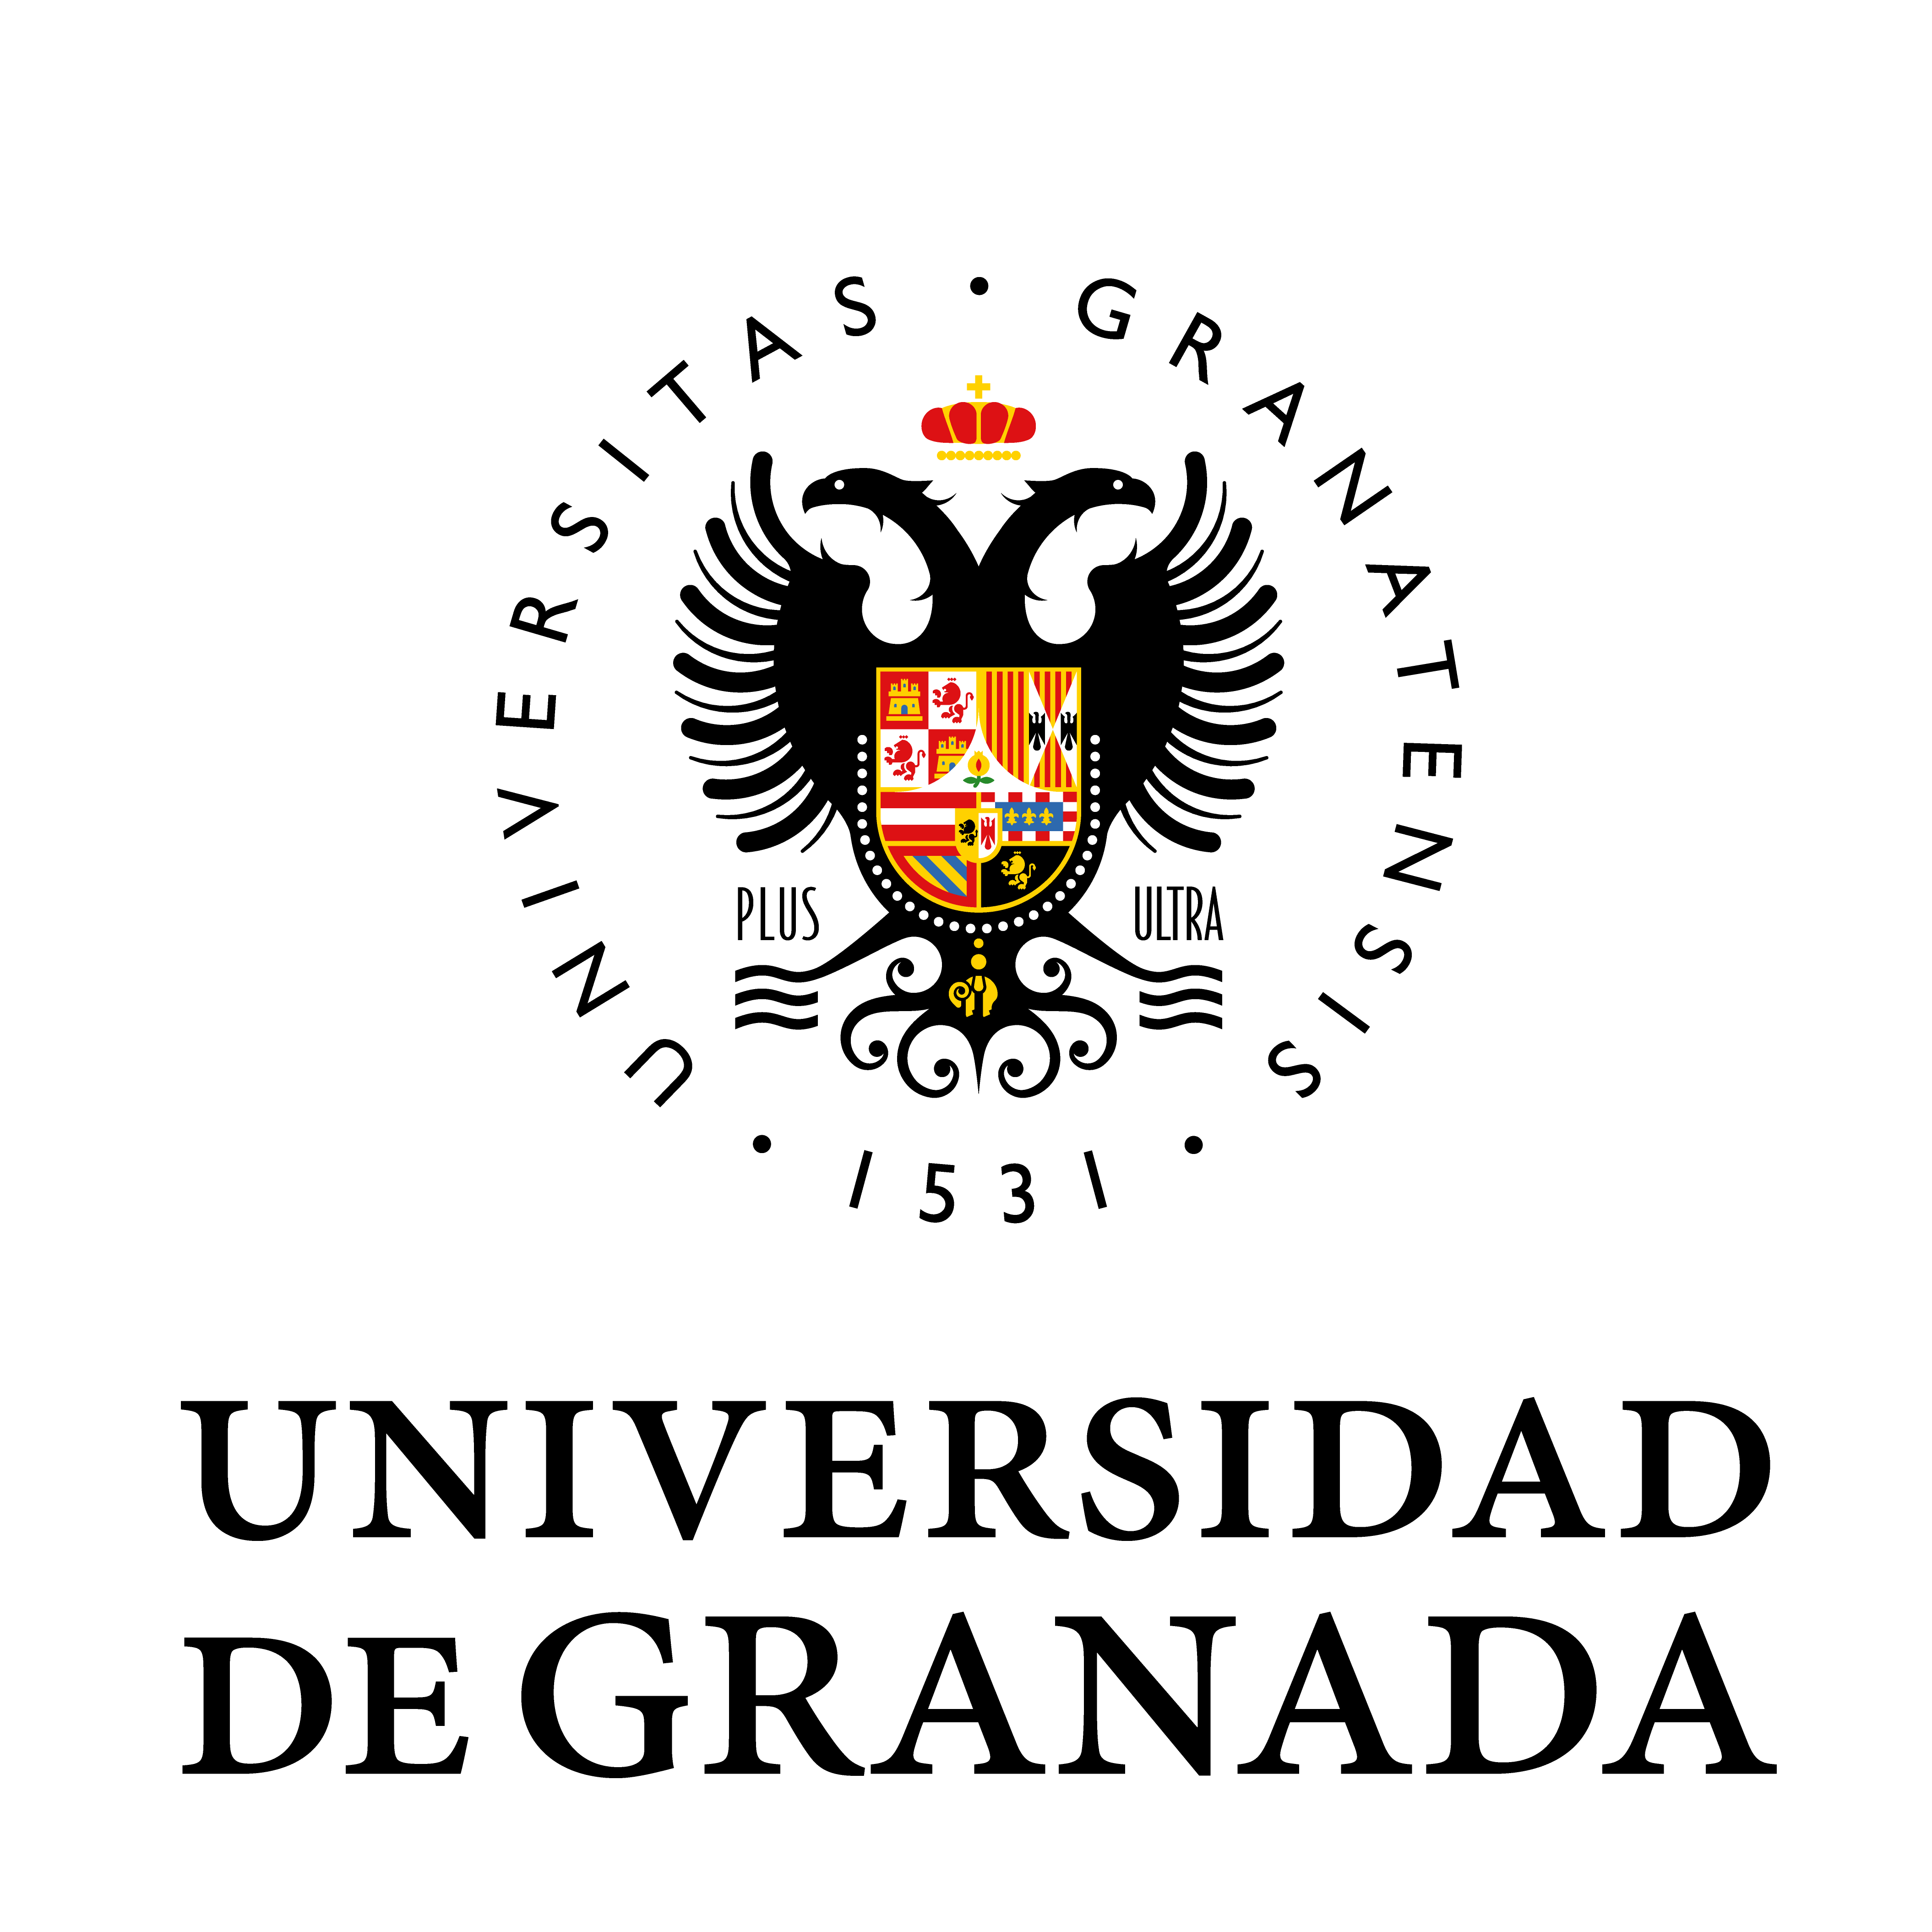
\includegraphics[width=0.4\textwidth]{escudo.png}\\[2cm] % logo arriba
    {\Huge TEMA 3}\\[1.5em]
    {\Huge Introducción a la Resistencia de Materiales}\\[2em]
}
\vspace{2em}
\author{\Large Pérez Hita, Christian \\[1em]}
\vspace{1cm}
\date{13 de octubre de 2026}

\begin{document}
\spanishdeactivate{.<>}
\setcounter{tocdepth}{3}
\maketitle
\newpage

\pdfbookmark[section]{\contentsname}{contenidos}
\tableofcontents
\pagebreak

\graphicspath{ {./Imagenes/} }

\setcounter{chapter}{2} % Para que empiece como Capítulo 3
% !TeX root = ../apuntes.tex
\chapter{Introducción a la Resistencia de Materiales}

\section{Objeto y Fundamentos de la Resistencia de Materiales}

Los cuerpos y elementos estructurales están compuestos a nivel microscópico por átomos enlazados entre sí a distancias de equilibrio interatómico. En las estructuras e instalaciones de ingeniería, estos cuerpos se encuentran vinculados al entorno mediante \textbf{sustentaciones, apoyos o ligaduras}.

\begin{figure}[H]
    \centering
    \adjustbox{max width=0.95\textwidth}{%
        \begin{tikzpicture}[node distance=2.2cm, auto, >=Latex]
            \node [draw, rectangle, rounded corners, fill=blue!10, text width=4.5cm, align=center, thick] (fuerza) {\textbf{Acción de Fuerzas Exteriores}\\(Cargas de servicio y peso propio)};
            \node [draw, rectangle, rounded corners, fill=yellow!15, text width=4.8cm, align=center, thick, right=2.5cm of fuerza] (transmision) {\textbf{Transmisión Interatómica}\\(Las fuerzas se transmiten átomo a átomo hasta la cimentación)};
            \node [draw, rectangle, rounded corners, fill=red!10, text width=4.5cm, align=center, thick, below=1.8cm of transmision] (deformacion) {\textbf{Deformación del Sólido}\\(Los átomos varían su distancia relativa: tracción/compresión)};
            \node [draw, rectangle, rounded corners, fill=green!10, text width=4.5cm, align=center, thick, below=1.8cm of fuerza] (equilibrio) {\textbf{Posición de Equilibrio Final}\\(Cesan los movimientos relativos)};

            \draw [->, line width=1.2pt] (fuerza) -- (transmision);
            \draw [->, line width=1.2pt] (transmision) -- (deformacion);
            \draw [->, line width=1.2pt] (deformacion) -- (equilibrio);
            \draw [->, line width=1.2pt, dashed] (equilibrio) -- node[midway, left=4pt, align=center] {\textit{Estado de estudio}} (fuerza);
        \end{tikzpicture}%
    }
    \caption{Mecanismo físico de respuesta tensional y deformacional de un sólido sometido a cargas.}
    \label{fig:respuesta_solido}
\end{figure}

Alcanzada la posición final de equilibrio estable, el análisis resistente persigue dos objetivos fundamentales:
\begin{itemize}
    \item Determinar las \textbf{fuerzas exteriores} aplicadas y las \textbf{fuerzas interiores} que mantienen la integridad y cohesión del cuerpo.
    \item Calcular las \textbf{deformaciones y desplazamientos} que describen el cambio de configuración geométrica del sólido.
\end{itemize}

\subsection{Mecánica, Teoría de la Elasticidad y Resistencia de Materiales}
Dentro de la Física y la Ingeniería Mecánica se distinguen tres niveles de aproximación:
\begin{enumerate}
    \item \textbf{Mecánica General:} Parte de la física que estudia el movimiento y reposo de los cuerpos bajo la acción de fuerzas, considerando prioritariamente el modelo de \textbf{sólido rígido indeformable}.
    \item \textbf{Teoría de la Elasticidad:} Rama de la mecánica de medios continuos que estudia los sólidos deformables elásticos. Calcula de forma matemáticamente rigurosa y tridimensional las funciones continuas de tensión y deformación en todos y cada uno de los puntos del sólido. Su elevada complejidad analítica hace que solo admita \textbf{solución exacta en geometrías muy limitadas}.
    \item \textbf{Resistencia de Materiales:} Disciplina técnica que combina los principios generales de la Elasticidad con una serie de \textbf{hipótesis simplificativas contrastadas por la experiencia}. Modela las estructuras complejas a partir de elementos prismáticos sencillos (\textbf{prismas mecánicos}), calculando esfuerzos, tensiones medias, deformaciones y desplazamientos seccionales con suficiente precisión para el diseño y la práctica ingenieril.
\end{enumerate}

\begin{figure}[H]
    \centering
    \adjustbox{max width=0.95\textwidth}{%
        \begin{tikzpicture}[>=Latex]
            \node [draw, rectangle, rounded corners, fill=blue!10, text width=5.2cm, align=center, thick] (elast) {\textbf{Principios Generales de la Elasticidad}};
            \node [draw, rectangle, rounded corners, fill=yellow!15, text width=5.2cm, align=center, thick, below=1.2cm of elast] (hip) {\textbf{Hipótesis Simplificativas}\\(Contrastadas por la experiencia)};
            \node [draw, rectangle, rounded corners, fill=green!15, text width=5.5cm, align=center, thick, right=2.8cm of elast, yshift=-1.1cm] (rm) {\textbf{Resistencia de Materiales}\\\small Estudio de piezas prismáticas:\\Resistencia, Rigidez y Estabilidad};

            \draw [->, line width=1.5pt] (elast) -| (rm);
            \draw [->, line width=1.5pt] (hip) -| (rm);
        \end{tikzpicture}%
    }
    \caption{Fundamento conceptual de la Resistencia de Materiales.}
    \label{fig:fundamento_rm}
\end{figure}

\subsection{Tipología de problemas en Resistencia de Materiales}
En el ejercicio profesional del ingeniero químico y mecánico se abordan dos tipos de problemas:
\begin{table}[H]
    \centering
    \caption{Clasificación de los problemas básicos en Resistencia de Materiales.}
    \adjustbox{max width=\textwidth}{%
        \begin{tabular}{lll}
            \toprule
            \textbf{Tipo de Problema}                                             & \textbf{Datos de Partida} & \textbf{Objetivo a Determinar} \\
            \midrule
            \textbf{De Dimensionamiento}                                          &
            \begin{tabular}{l}
                $\bullet$ Solicitaciones / Cargas de servicio \\
                $\bullet$ Propiedades del material ($\sigma_{\text{adm}}, E, \nu$)
            \end{tabular} &
            \begin{tabular}{l}
                Calcular las dimensiones de la sección transversal \\
                para que el elemento sea \textbf{seguro y económico}.
            \end{tabular}                                                                               \\
            \midrule
            \textbf{De Comprobación}                                              &
            \begin{tabular}{l}
                $\bullet$ Geometría y dimensiones existentes \\
                $\bullet$ Propiedades del material           \\
                $\bullet$ Solicitaciones aplicadas
            \end{tabular}                       &
            \begin{tabular}{l}
                Verificar que las tensiones y deformaciones reales \\
                no superan los límites admisibles (\textbf{servicio seguro}).
            \end{tabular}                                                                       \\
            \bottomrule
        \end{tabular}%
    }
    \label{tab:tipos_problemas}
\end{table}

\subsection{Las Variables y el Diagrama de Tonti}
Las magnitudes que intervienen en el análisis elasto-resistente se estructuran y relacionan a través del denominado \textbf{Diagrama de Tonti}:

\begin{figure}[H]
    \centering
    \adjustbox{max width=0.98\textwidth}{%
        \begin{tikzpicture}[>=Latex]
            % Nodos superiores
            \node [draw, rectangle, rounded corners, fill=red!10, text width=4.3cm, align=center, thick] (fuerzas) at (0,4.6) {\textbf{Fuerzas / Momentos}\\\small(Acciones exteriores)};
            \node [draw, rectangle, rounded corners, fill=blue!10, text width=4.3cm, align=center, thick] (desplaz) at (8.2,4.6) {\textbf{Desplazamientos}\\\small($u, v, w, \theta_x, \theta_y, \theta_z$)};

            % Nodos inferiores
            \node [draw, rectangle, rounded corners, fill=orange!15, text width=4.3cm, align=center, thick] (tensiones) at (0,0) {\textbf{Esfuerzos / Tensiones}\\\small($N, Q, M_f, T \;\longleftrightarrow\; \sigma, \tau$)};
            \node [draw, rectangle, rounded corners, fill=cyan!15, text width=4.3cm, align=center, thick] (deform) at (8.2,0) {\textbf{Deformaciones}\\\small($\varepsilon, \gamma$)};

            % Flechas verticales con texto espaciado
            \draw [<->, line width=1.4pt, red!70!black] (fuerzas) -- node[midway, left=8pt, text width=3.3cm, align=right] {\small\textbf{Ec. de Equilibrio}\\(Estático y Elástico)} (tensiones);
            \draw [<->, line width=1.4pt, blue!70!black] (desplaz) -- node[midway, right=8pt, text width=3.3cm, align=left] {\small\textbf{Ec. de Compatibilidad}\\Geométrica} (deform);

            % Flecha horizontal con texto con suficiente altura
            \draw [<->, line width=1.4pt, green!60!black] (tensiones) -- node[midway, above=8pt, align=center] {\textbf{Leyes de Comportamiento}\\\footnotesize(Ley de Hooke: $\sigma = E\cdot\varepsilon,\; \tau = G\cdot\gamma$)} (deform);
        \end{tikzpicture}%
    }
    \caption{Diagrama de Tonti: interrelación entre magnitudes estáticas, tensionales, cinemáticas y constitutivas.}
    \label{fig:diagrama_tonti}
\end{figure}

\imp{
    \textbf{Objetivos de diseño en el cálculo de estructuras:}
    \begin{itemize}
        \item \textbf{Estructuras Seguras (Resistencia):} A partir de las solicitaciones exteriores $\longrightarrow$ Esfuerzos $\longrightarrow$ Tensiones $\longrightarrow$ \textbf{Comparar con Tensiones Admisibles} ($\sigma_{\text{max}} \leq \sigma_{\text{adm}}$).
        \item \textbf{Estructuras Útiles (Funcionalidad/Rigidez):} A partir de las solicitaciones exteriores $\longrightarrow$ Esfuerzos $\longrightarrow$ Deformaciones $\longrightarrow$ Desplazamientos $\longrightarrow$ \textbf{Comparar con Desplazamientos Límites} ($\delta_{\text{max}} \leq \delta_{\text{adm}}$).
        \item \textbf{Estructuras Económicas:} Minimizar el consumo de material y costes de conformado cumpliendo los dos criterios de seguridad y utilidad.
    \end{itemize}
}

%=============================================================================
\section{Sólido Deformable Elástico y Prisma Mecánico}

\subsection{Tipos de sólidos en mecánica}
\begin{enumerate}
    \item \textbf{Sólido Rígido:} Modelo ideal indeformable. Su condición de equilibrio exige que no experimente desplazamientos ni giros:
          \begin{align}
              \text{Traslaciones impedidas:} & \quad R_x = 0, \quad R_y = 0, \quad R_z = 0 \implies \sum \vec{F} = \vec{0}            \\
              \text{Rotaciones impedidas:}   & \quad M_{ox} = 0, \quad M_{oy} = 0, \quad M_{oz} = 0 \implies \sum \vec{M}_o = \vec{0}
          \end{align}
    \item \textbf{Sólido Elástico Deformable:} Sólido que se deforma bajo la acción de cargas y recupera íntegramente su geometría original al descargarse. Se modeliza bajo tres hipótesis:
          \begin{itemize}
              \item \textbf{Isotropía:} Las propiedades elásticas son iguales en todas las direcciones espaciales.
              \item \textbf{Homogeneidad:} La composición y propiedades mecánicas son idénticas en cualquier punto del volumen.
              \item \textbf{Continuidad:} La materia llena el espacio de forma continua sin poros, oquedades ni fisuras.
          \end{itemize}
    \item \textbf{Sólido Verdadero / Real:} Los materiales reales son heterogéneos a escala microscópica, anisótropos y presentan discontinuidades y tensiones residuales.
\end{enumerate}

\subsection{Definición y geometría del Prisma Mecánico}

\dfn{Prisma Mecánico}{Cuerpo geométrico generado por una superficie plana $\Omega$ (sección transversal) cuyo baricentro o centro de gravedad $G$ recorre una curva continua orientada denominada \textbf{línea directriz} ($C$), manteniéndose el plano de la sección en todo momento normal a la directriz.}

\begin{figure}[H]
    \centering
    \adjustbox{max width=0.95\textwidth}{%
        \begin{tikzpicture}[scale=1.1, >=Latex]
            % Directriz
            \draw[thick, blue!80!black, dashed] (-3.8,-0.6) to[out=25,in=205] (0,0) to[out=25,in=190] (4.8,0.7);
            \node[blue!80!black, above=2pt] at (3.0,0.6) {$C$ (Directriz)};
            \filldraw[black] (-3.8,-0.6) circle (1.5pt) node[left=2pt] {$G_1$};
            \filldraw[black] (4.8,0.7) circle (1.5pt) node[right=2pt] {$G_2$};

            % Contorno exterior del prisma
            \draw[thick] (-3.8,0.8) to[out=25,in=170] (0,1.4) to[out=-10,in=190] (4.8,1.8);
            \draw[thick] (-3.8,-2.0) to[out=25,in=195] (0,-1.4) to[out=15,in=190] (4.8,-0.4);
            \draw[thick] (-3.8,0.8) arc (90:270:0.4cm and 1.4cm);
            \draw[thick, dashed] (-3.8,-2.0) arc (-90:90:0.4cm and 1.4cm);
            \draw[thick] (4.8,0.7) ellipse (0.5cm and 1.1cm);

            % Sección transversal Omega
            \draw[thick, fill=gray!25, fill opacity=0.75] (0,0) ellipse (0.7cm and 1.4cm);
            \node at (0.25,0.9) {$\Sigma$};
            \node[below right=2pt] at (0.4,-1.1) {$\Omega$};

            % Centro de gravedad G
            \filldraw[black] (0,0) circle (2pt) node[below left=2pt] {$G$};

            % Triedro intrínseco local (ejes x, y, z)
            \draw[->, line width=1.5pt, red!80!black] (0,0) -- (2.3,0.38) node[right=2pt] {$x$};
            \draw[->, line width=1.5pt, green!60!black] (0,0) -- (0,2.3) node[above=2pt] {$y$};
            \draw[->, line width=1.5pt, cyan!80!black] (0,0) -- (-1.1,-0.9) node[below left=2pt] {$z$};
        \end{tikzpicture}%
    }
    \caption{Geometría de un prisma mecánico y triedro intrínseco local $(G, x, y, z)$.}
    \label{fig:prisma_mecanico_triedro}
\end{figure}

\subsection{Clasificación de los prismas mecánicos en ingeniería}
\begin{enumerate}
    \item \textbf{Barra o Viga:} Las dimensiones transversales de la sección ($b, h$) son muy pequeñas en comparación con la longitud de su línea media ($L$). Permite simplificar el cálculo tridimensional a un modelo unidimensional/bidimensional:
          \begin{equation}
              L > 10 - 20 \cdot D \quad (D = \text{canto o dimensión transversal})
          \end{equation}
    \item \textbf{Placa:} Prisma delimitado por dos superficies planas paralelas donde la distancia entre ambas (\textbf{espesor} $e$) es muy pequeña frente a las otras dos dimensiones en planta ($L > 40\cdot e$). Se define respecto a su \textit{superficie media}.
    \item \textbf{Lámina o Cáscara:} Estructura bidimensional semejante a la placa pero cuyas superficies delimitadoras son \textbf{curvas} (bóvedas, depósitos cilíndricos y esféricos).
\end{enumerate}

%=============================================================================
\section{Principios Generales de la Resistencia de Materiales}

\subsection{1. Principio de Rigidez Relativa (Teoría de Primer Orden)}
\textbf{Hipótesis de pequeñas deformaciones y desplazamientos:} Las deformaciones que experimentan las piezas elásticas son tan reducidas que \textbf{las ecuaciones de equilibrio estático se formulan sobre la geometría inicial indeformada} del sistema sin cometer errores apreciables.

\subsection{2. Principio de Superposición}
Se fundamenta en la combinación de la \textbf{Ley de Hooke (comportamiento elástico-lineal)} y el \textbf{Principio de Rigidez Relativa}:
\dfn{Principio de Superposición}{El efecto producido por un sistema complejo de fuerzas actuando conjuntamente es igual a la suma de los efectos producidos por cada una de las fuerzas actuando de manera independiente.}
\imp{Bajo condiciones elásticas y pequeñas deformaciones, el orden de aplicación de las cargas no altera el estado final de tensiones ni de deformaciones.}

\subsection{3. Principio de Saint-Venant}
\dfn{Principio de Saint-Venant}{Salvo en las inmediaciones directas del punto de aplicación de las cargas, los estados tensionales y deformacionales producidos por dos sistemas de cargas estáticamente equivalentes son prácticamente idénticos a una distancia suficiente ($x \geq d_{\text{transversal}}$).}

\begin{figure}[H]
    \centering
    \adjustbox{max width=0.92\textwidth}{%
        \begin{tikzpicture}[scale=0.9, >=Latex]
            % Caso 1: Carga puntual concentrada P
            \draw[thick, fill=blue!5] (0,0) rectangle (2.5,4);
            \draw[<-, line width=1.5pt, red!80!black] (1.25,4) -- (1.25,5.2) node[above=2pt] {$P$ (Puntual)};

            % Flechas de tension en la base
            \foreach \x in {0.2,0.6,1.0,1.4,1.8,2.2} {
                    \draw[->, line width=1pt, blue!70!black] (\x,0) -- (\x,-0.7);
                }
            % Texto debajo de las flechas (sin superposicion)
            \node[below=4pt] at (1.25,-0.75) {$\displaystyle \sigma = \frac{P}{\Omega}$};

            % Equivalencia con separacion adecuada
            \draw[<->, line width=1.8pt, green!60!black] (3.4,2) -- (6.0,2);
            \node[above=4pt, text width=2.8cm, align=center] at (4.7,2) {\small\textbf{Sistemas}\\\small\textbf{Equivalentes}};

            % Caso 2: Carga distribuida uniforme
            \draw[thick, fill=blue!5] (6.8,0) rectangle (9.3,4);
            \foreach \x in {7.0,7.4,7.8,8.2,8.6,9.0} {
                    \draw[<-, line width=1pt, red!80!black] (\x,4) -- (\x,4.8);
                }
            \draw[line width=1pt, red!80!black] (7.0,4.8) -- (9.0,4.8) node[midway, above=2pt] {$P$ (Distribuida)};

            % Flechas de tension en la base
            \foreach \x in {7.0,7.4,7.8,8.2,8.6,9.0} {
                    \draw[->, line width=1pt, blue!70!black] (\x,0) -- (\x,-0.7);
                }
            % Texto debajo de las flechas (sin superposicion)
            \node[below=4pt] at (8.05,-0.75) {$\displaystyle \sigma = \frac{P}{\Omega}$};
        \end{tikzpicture}%
    }
    \caption{Principio de Saint-Venant: distribución uniforme de tensiones $\sigma = P/\Omega$ a una distancia representativa de la sección de carga.}
    \label{fig:saint_venant}
\end{figure}

\subsection{4. Hipótesis de Navier-Bernoulli (Secciones Planas)}
\dfn{Hipótesis de Navier-Bernoulli}{Las secciones planas y perpendiculares a la línea directriz de una pieza antes de la deformación permanecen planas y normales a la directriz deformada después de la flexión.}
\nt{Esta hipótesis es estrictamente válida para vigas esbeltas ($L > 10\cdot h$). Para vigas de gran canto ($L < 10\cdot h$) o bajo elevados esfuerzos cortantes, las secciones sufren alabeo transversal y debe aplicarse la teoría de vigas gruesas de Timoshenko.}

%=============================================================================
\section{Solicitaciones Exteriores, Ligaduras y Reacciones}

\subsection{Clasificación de las solicitaciones exteriores}
Las acciones mecánicas exteriores se dividen en:
\begin{enumerate}
    \item \textbf{Acciones directas o Cargas ($F + M$):}
          \begin{itemize}
              \item \textit{Fuerzas de volumen ($F_v$):} Actúan sobre cada elemento diferencial de masa (peso propio, fuerzas centrífugas).
              \item \textit{Fuerzas de superficie ($F_\Omega$):} Actúan sobre las caras exteriores (presiones hidrostáticas, empuje de viento).
              \item \textit{Momentos aplicados:} Pares de fuerzas torsores o flectores.
              \item \textit{Distribución:} Cargas concentradas (puntuales) o cargas repartidas (uniformes o variables).
          \end{itemize}
    \item \textbf{Fuerzas de Reacción ($F + M$):} Fuerzas y momentos que los apoyos ejercen sobre el sólido para coaccionar sus grados de libertad:
          \begin{itemize}
              \item Si se restringe un \textbf{desplazamiento}, aparece una \textbf{fuerza de reacción} en la dirección del movimiento impedido.
              \item Si se restringe un \textbf{giro}, aparece un \textbf{momento de reacción} que se opone a dicho giro.
          \end{itemize}
\end{enumerate}

\subsection{Ligaduras y reacciones en 3D y 2D}
\begin{itemize}
    \item \textbf{En el espacio tridimensional (3D):} Un punto libre posee \textbf{6 grados de libertad} (3 desplazamientos $u, v, w$ y 3 giros $\theta_x, \theta_y, \theta_z$).
          \begin{itemize}
              \item \textbf{Empotramiento 3D:} Restringe los 6 grados de libertad $\implies \mathbf{6\text{ Reacciones}}$ (3 Fuerzas $R_x, R_y, R_z$ y 3 Momentos $M_{tx}, M_{fy}, M_{fz}$).
              \item \textbf{Rótula esférica / Articulación 3D:} Restringe los 3 desplazamientos $\implies \mathbf{3\text{ Reacciones de fuerza}}$ ($R_x, R_y, R_z$).
          \end{itemize}
    \item \textbf{En el plano bidimensional (2D):} Un punto posee \textbf{3 grados de libertad} (2 desplazamientos $u, v$ y 1 giro $\theta_z$).
\end{itemize}

\begin{table}[H]
    \centering
    \caption{Tipos de enlaces en estructuras planas (2D) y reacciones originadas.}
    \adjustbox{max width=\textwidth}{%
        \begin{tabular}{lcp{6cm}c}
            \toprule
            \textbf{Tipo de Apoyo}                             & \textbf{Símbolo 2D}                                                  & \textbf{Movimientos Permitidos / Coaccionados} & \textbf{Reacciones} \\
            \midrule
            \textbf{Apoyo Móvil / Carrito}                     & \begin{tikzpicture}[scale=0.5]
                                                                     \draw[thick] (0,0.4) -- (1,0.4) -- (0.5,1) -- cycle;
                                                                     \draw[thick] (0.2,0.2) circle (0.15);
                                                                     \draw[thick] (0.8,0.2) circle (0.15);
                                                                     \draw[line width=1pt] (-0.3,0) -- (1.3,0);
                                                                 \end{tikzpicture}                 &
            \begin{tabular}{l}
                $\bullet$ Permite traslación horizontal ($u$) \\
                $\bullet$ Permite giro ($\theta_z$)           \\
                $\bullet$ Impide traslación vertical ($v$)
            \end{tabular}   & \textbf{1 Fuerza} ($R_y$)                                                                                                                                                    \\
            \midrule
            \textbf{Articulación Fija}                         & \begin{tikzpicture}[scale=0.5]
                                                                     \draw[thick] (0,0) -- (1,0) -- (0.5,1) -- cycle;
                                                                     \draw[line width=1pt] (-0.3,0) -- (1.3,0);
                                                                     \foreach \x in {-0.2,0.1,0.4,0.7,1.0} \draw (\x,0) -- (\x-0.2,-0.3);
                                                                 \end{tikzpicture} &
            \begin{tabular}{l}
                $\bullet$ Permite giro en el plano ($\theta_z$) \\
                $\bullet$ Impide traslación horizontal ($u$)    \\
                $\bullet$ Impide traslación vertical ($v$)
            \end{tabular} & \textbf{2 Fuerzas} ($R_x, R_y$)                                                                                                                                                  \\
            \midrule
            \textbf{Empotramiento}                             & \begin{tikzpicture}[scale=0.5]
                                                                     \draw[line width=1.5pt] (0,-0.5) -- (0,1.5);
                                                                     \foreach \y in {-0.4,0.1,0.6,1.1} \draw (0,\y) -- (-0.3,\y-0.2);
                                                                     \draw[thick] (0,0.5) -- (1.2,0.5);
                                                                 \end{tikzpicture}     &
            \begin{tabular}{l}
                $\bullet$ Impide traslación horizontal ($u$) \\
                $\bullet$ Impide traslación vertical ($v$)   \\
                $\bullet$ Impide giro en el plano ($\theta_z$)
            \end{tabular}    & \textbf{3 Reacciones} ($R_x, R_y, M_z$)                                                                                                                                       \\
            \bottomrule
        \end{tabular}%
    }
    \label{tab:apoyos_2d}
\end{table}
Tambien aparecen solicitaciones interiores que son los esfuerzos (lo que pasa por dentro).
\subsection{Clasificación estática de los sistemas estructurales}
Sea $R$ el número total de reacciones incógnita y $E$ el número de ecuaciones de equilibrio estático independientes ($E=3$ en 2D, $E=6$ en 3D, más posibles ecuaciones de despiece por rótulas internas):
\begin{itemize}
    \item \textbf{Sistema Isostático ($R = E$):} Las ecuaciones de la estática son estrictamente suficientes para determinar todas las reacciones de enlace.
    \item \textbf{Sistema Hipoestático ($R < E$):} El número de coacciones es insuficiente; la estructura posee movilidad interna y se comporta como un \textbf{mecanismo} (ejemplo en una viga con 2 ligaduras tipo apoyo móvil se traslada la viga horizontalmente al haber 2 incognitas R1 R2 y 3 ecuaciones).
    \item \textbf{Sistema Hiperestático ($R > E$):} El número de reacciones supera al de ecuaciones de equilibrio estático. El sistema posee ligaduras redundantes y se define el \textbf{Grado de Hiperestaticidad ($GH$)}:
          \begin{equation}
              GH = R - E
              \label{eq:grado_hiperestaticidad}
          \end{equation}
          Para resolver un sistema hiperestático es obligatorio plantear $GH$ \textbf{ecuaciones adicionales de compatibilidad de deformaciones}.
\end{itemize}
\nt{Nosotros trabajaremos con los sistemas Isostaticos, cuando hay una rotula siempre hay una ecuación mas}
%=============================================================================
\section{Concepto Riguroso de Tensión}
\nt{Si un cuerpo esta en equilibrio cualquier parte interna de el tambien lo esta si dieramos un corte al prisma mostrado, la seccion cortada estaria tambien en equilibrio, Condicion de equilibrio elastico, las solicitaciones exteriores estan en equilibrio con todas las interiores (esto es importante por que con ello calcularemos los esfuerzos)} %!revisar figura papel 


Consideremos un cuerpo continuo en equilibrio seccionado imaginariamente por una superficie plana $\Omega$. En el entorno de un punto $P$ de la sección, sobre un elemento diferencial de área $\Delta \Omega$ con vector normal unitario $\vec{n}$, actúa una fuerza interna resultante $\Delta \vec{f}$.

\dfn{Vector Tensión}{Límite del cociente entre la fuerza elemental interna y el área cuando ésta tiende a cero:}
\begin{equation}
    \vec{t} = \vec{\sigma} = \lim_{\Delta \Omega \to 0} \left( \frac{\Delta \vec{f}}{\Delta \Omega} \right) = \frac{d\vec{f}}{d\Omega}
    \label{eq:vector_tension}
\end{equation}
% !!!!!!!!!!!!!!!!!!!!!!!!!!!  arreglar el error vissual de lim  !!!!!!!!!!!!!!!!!!!!!!!!!!!

\begin{figure}[H]
    \centering
    \adjustbox{max width=0.92\textwidth}{%
        \begin{tikzpicture}[scale=1.1, >=Latex]
            % Superficie de corte
            \draw[thick, fill=cyan!15] (0,0) ellipse (1.5cm and 2.2cm);
            \node[above=4pt] at (0,2.2) {Sección transversal $\Omega$};

            % Elemento de area dOmega
            \draw[thick, fill=yellow!40] (0.3,0.3) rectangle (0.8,0.8);
            \node[below left=1pt] at (0.3,0.3) {$d\Omega$};

            % Vector tension total
            \draw[->, line width=1.5pt, red!80!black] (0.55,0.55) -- (2.4,1.8) node[above right=2pt] {$\vec{t} = \vec{\sigma}$ (Vector Tensión)};

            % Descomposicion intrinseca
            \draw[->, line width=1.3pt, blue!80!black] (0.55,0.55) -- (0.55,2.1) node[left=2pt] {$\vec{\sigma}_n$ (Tensión normal)};
            \draw[->, line width=1.3pt, green!60!black] (0.55,0.55) -- (2.2,0.55) node[below right=2pt] {$\vec{\tau}$ (Tensión tangencial)};
            \draw[dashed, gray] (2.2,0.55) -- (2.4,1.8) -- (0.55,2.1);
        \end{tikzpicture}%
    }
    \caption{Vector tensión en un punto y sus componentes intrínsecas normal ($\sigma_n$) y tangencial ($\tau$).}
    \label{fig:componentes_tension}
\end{figure}

\textbf{Características del vector tensión:}
\begin{itemize}
    \item Cada vector tensión está unívocamente asociado a la orientación del plano de corte ($\vec{n}$).
    \item En general, el vector $\vec{t}$ no es perpendicular al plano de la sección.
    \item \textbf{Componente normal ($\sigma_n$):} Proyección perpendicular a la sección (produce tracción o compresión, es decir produce cambios de tamaño deformacion por dilatacion).
    \item \textbf{Componente tangencial ($\tau$):} Proyección contenida en el plano de la sección (produce cizalladura o cortadura, produce deformacion por distorsion angular).
    \item \textbf{Módulo del vector tensión:} $|\vec{t}| = \sqrt{\sigma_n^2 + \tau^2}$.
    \item \textbf{Unidades de tensión:} $\text{N/m}^2 = \text{Pa}$, empleándose en ingeniería:
          \begin{equation}
              1\text{ MPa} = 1\text{ N/mm}^2 = 10\text{ kp/cm}^2
          \end{equation}
\end{itemize}

%=============================================================================
\section{Concepto de Deformación y Ley de Hooke Generalizada}

\subsection{Componentes de la deformación}
Bajo la acción de cargas, un paralelepípedo elemental de dimensiones $dx \cdot dy \cdot dz$ experimenta un movimiento general compuesto por:
\begin{equation}
    \text{Movimiento total} = \text{Traslación de sólido rígido} + \text{Rotación de sólido rígido} + \textbf{Deformación propiamente dicha}
\end{equation}
La deformación propiamente dicha se descompone en:
\begin{enumerate}
    \item \textbf{Dilatación o Deformación longitudinal unitaria ($\varepsilon$):} Cambio de tamaño (variación de longitud por unidad de longitud) manteniendo los ángulos rectos iniciales:
          \begin{equation}
              \varepsilon_x = \frac{\Delta L_x}{L_{0x}}
          \end{equation}
    \item \textbf{Distorsión angular ($\gamma$):} Cambio de forma geométrica (variación del ángulo recto original entre dos direcciones ortogonales) a volumen constante:
          \begin{equation}
              \gamma_{xy} = \frac{\pi}{2} - \theta'_{xy} \quad [\text{radianes}]
          \end{equation}
\end{enumerate}

\subsection{Ley de Hooke Uniaxial y Coeficiente de Poisson}
Para un ensayo de tracción uniaxial en la dirección $X$ ($\sigma_x \neq 0, \sigma_y = \sigma_z = 0$):
\begin{align}
    \text{Deformación longitudinal:}    & \quad \varepsilon_x = \frac{\sigma_x}{E}                                                                                                            \\
    \text{Deformaciones transversales:} & \quad \varepsilon_y = -\nu \cdot \varepsilon_x = -\nu \frac{\sigma_x}{E}, \qquad \varepsilon_z = -\nu \cdot \varepsilon_x = -\nu \frac{\sigma_x}{E}
\end{align}
donde $E$ es el \textbf{módulo de elasticidad longitudinal (Módulo de Young)} y $\nu$ es el \textbf{coeficiente de Poisson} ($\nu \approx 0.28 - 0.33$ en aceros).

Para tensiones tangenciales puras:
\begin{equation}
    \tau = G \cdot \gamma
\end{equation}
donde $G$ es el \textbf{módulo de elasticidad transversal o de cortadura}, relacionado elásticamente con $E$ y $\nu$ mediante:
\begin{equation}
    G = \frac{E}{2(1 + \nu)}
    \label{eq:modulo_cizalladura_G}
\end{equation}

\subsection{Ley de Hooke Generalizada (Estado Tensional Tridimensional)}
Aplicando el principio de superposición de efectos a un elemento paralelepípedo sometido a un tensor de tensiones general:
\begin{equation}
    \begin{cases}
        \varepsilon_x = \dfrac{\sigma_x}{E} - \dfrac{\nu}{E}(\sigma_y + \sigma_z), & \gamma_{xy} = \dfrac{\tau_{xy}}{G} \\[10pt]
        \varepsilon_y = \dfrac{\sigma_y}{E} - \dfrac{\nu}{E}(\sigma_z + \sigma_x), & \gamma_{yz} = \dfrac{\tau_{yz}}{G} \\[10pt]
        \varepsilon_z = \dfrac{\sigma_z}{E} - \dfrac{\nu}{E}(\sigma_x + \sigma_y), & \gamma_{zx} = \dfrac{\tau_{zx}}{G}
    \end{cases}
    \label{eq:hooke_generalizada}
\end{equation}

%=============================================================================
\section{Concepto de Esfuerzo y Criterio de Signos}

\subsection{Definición vectorial de esfuerzos}
Al realizar un corte transversal a un prisma mecánico por una sección $\Omega$, las fuerzas que la parte derecha ejerce sobre la parte izquierda se reducen en el baricentro $G$ a una \textbf{fuerza resultante} $\vec{R}$ y a un \textbf{momento resultante} $\vec{M}$:

\dfn{Esfuerzos Seccionales}{Componentes escalares de los vectores $\vec{R}$ y $\vec{M}$ proyectadas sobre los ejes del triedro intrínseco $(G, X, Y, Z)$:}
\begin{align}
    \vec{R} & = N\vec{i} + Q_y\vec{j} + Q_z\vec{k}       \\
    \vec{M} & = T\vec{i} + M_{fy}\vec{j} + M_{fz}\vec{k}
\end{align}

\begin{itemize}
    \item \textbf{Esfuerzo Axil ($N$):} Componente de $\vec{R}$ normal a la sección (eje $X$). Produce tracción ($N > 0$) o compresión ($N < 0$).
    \item \textbf{Esfuerzos Cortantes ($Q_y, Q_z$ o $T_y, T_z$):} Componentes de $\vec{R}$ contenidas en el plano de la sección (ejes $Y, Z$).
    \item \textbf{Momento Torsor ($T$ o $M_t$):} Componente de $\vec{M}$ alrededor del eje longitudinal $X$. Tiende a retorcer la barra sobre su directriz.
    \item \textbf{Momentos Flectores ($M_{fy}, M_{fz}$):} Componentes de $\vec{M}$ alrededor de los ejes transversales $Y$ y $Z$. Tienden a curvar la viga.
\end{itemize}
los momentos siempre son pares de esfuerzos o momentos, pero siempre van de 2 en 2
\subsection{Problemas planos (2D)}
En piezas simétricas con cargas contenidas en su plano medio, los esfuerzos activos se reducen a tres:
\begin{equation}
    \text{Axil } N \quad (\text{eje } X), \qquad \text{Cortante } Q \quad (\text{eje } Y), \qquad \text{Momento Flector } M_z \quad (\text{alrededor del eje } Z)
\end{equation}

\begin{figure}[H]
    \centering
    \adjustbox{max width=0.95\textwidth}{%
        \begin{tikzpicture}[scale=1.0, >=Latex]
            % AXIL POSITIVO
            \draw[thick] (0,0) rectangle (1.5,1);
            \draw[<-, line width=1.3pt, red!80!black] (-0.7,0.5) -- (0,0.5);
            \draw[->, line width=1.3pt, red!80!black] (1.5,0.5) -- (2.2,0.5);
            \node[below] at (0.75,-0.2) {\textbf{Axil (+)}: Tracción};

            % CORTANTE POSITIVO
            \draw[thick] (4,0) rectangle (5.5,1);
            \draw[->, line width=1.3pt, blue!80!black] (3.6,0.2) -- (3.6,1.0);
            \draw[->, line width=1.3pt, blue!80!black] (5.9,0.8) -- (5.9,0.0);
            \node[below] at (4.75,-0.2) {\textbf{Cortante (+)}};

            % MOMENTO FLECTOR POSITIVO
            \draw[thick] (8,0) rectangle (9.5,1);
            \draw[->, line width=1.3pt, green!60!black] (7.5,0.2) arc (-90:90:0.4);
            \draw[->, line width=1.3pt, green!60!black] (10.0,0.8) arc (90:270:0.4);
            \node[below] at (8.75,-0.2) {\textbf{Flector (+)}: Tracciona fibra inferior};
        \end{tikzpicture}%
    }
    \caption{Criterio de signos estándar para esfuerzos en vigas planas 2D.}
    \label{fig:criterio_signos_esfuerzos}
\end{figure}

%=============================================================================
\section{Relaciones Integrales entre Tensiones y Esfuerzos}

Las tensiones ($\sigma, \tau$) distribuidas en cada punto diferencial $dS$ de la sección transversal $S$ son estáticamente equivalentes a los esfuerzos resultantes ($N, Q, M, T$):

\begin{align}
    \text{Esfuerzo Axil:}                  & \quad N = \int_S \sigma_x \, dS \label{eq:int_axil}                                      \\[6pt]
    \text{Esfuerzo Cortante en $Y$:}       & \quad Q_y = T_y = \int_S \tau_{xy} \, dS \label{eq:int_qy}                               \\[6pt]
    \text{Esfuerzo Cortante en $Z$:}       & \quad Q_z = T_z = \int_S \tau_{xz} \, dS \label{eq:int_qz}                               \\[6pt]
    \text{Momento Torsor:}                 & \quad M_t = T = \int_S (\tau_{xz}\cdot y - \tau_{xy}\cdot z) \, dS \label{eq:int_torsor} \\[6pt]
    \text{Momento Flector respecto a $Y$:} & \quad M_{fy} = M_y = \int_S \sigma_x \cdot z \, dS \label{eq:int_my}                     \\[6pt]
    \text{Momento Flector respecto a $Z$:} & \quad M_{fz} = M_z = -\int_S \sigma_x \cdot y \, dS \label{eq:int_mz}
\end{align}

%=============================================================================
\section{Concepto de Seguridad Estructural}

En el diseño mecánico real, los cálculos analíticos y los ensayos de laboratorio están sujetos a \textbf{factores de incertidumbre}:
\begin{itemize}
    \item \textbf{Incertidumbres en la solicitación y modelo:} La geometría real fabricada difiere de la nominal de cálculo, las cargas y puntos de aplicación varían con el tiempo, y los métodos de cálculo contienen aproximaciones.
    \item \textbf{Incertidumbres en el material:} Los materiales reales presentan dispersión de propiedades, defectos microestructurales y los ensayos mecánicos tienen tolerancias de medición.
\end{itemize}

Para garantizar que la estructura nunca alcance el fallo bajo servicio, se aplican los \textbf{Coeficientes de Seguridad}:
\begin{enumerate}
    \item \textbf{Mayoración de cargas ($\gamma_f > 1$):} Define la \textbf{tensión de cálculo o de diseño} ($\sigma_d$):
          \begin{equation}
              \sigma_d = \sigma_{\text{max}} \cdot \gamma_f
          \end{equation}
    \item \textbf{Minoración de resistencia ($\gamma_s > 1$):} Define la \textbf{tensión admisible del material} ($\sigma_{\text{adm}}$) a partir del límite elástico ($\sigma_e$ o $\sigma_{0.2}$):
          \begin{equation}
              \sigma_{\text{adm}} = \frac{\sigma_e}{\gamma_s}
          \end{equation}
\end{enumerate}

\imp{
    \textbf{Condición fundamental de seguridad de cálculo:}
    \begin{equation}
        \sigma_d \leq \sigma_{\text{adm}} \iff \sigma_{\text{max}} \cdot \gamma_f \leq \frac{\sigma_e}{\gamma_s}
        \label{eq:condicion_seguridad_final}
    \end{equation}
}
Valores caracteristicos son los reales los de calculo son los minorados o mayorados, se hace tanto la minoracion como la miyoracion para tener seguridad.
%========================================================
%Resumen
\section{Resumen}
\ex{Viga con forjado}{si en una viga con dos soportes fijos en los extremos se le pone una carga y la deformacion que tiene por los esfuerzos es muy amplia no sirve}
% Sólido elástico completo y corte
Solido cuerpo elástico: en cualquier estructura en equilibrio, cualquier parte de ella que aislemos también debe estar en equilibrio ($\sum F_x = 0, \sum F_y = 0, \sum M = 0$). Para ello, en la superficie del corte deben aparecer las fuerzas internas ($f_1, f_2, \dots$) que compensan las solicitaciones exteriores.

\begin{figure}[H]
    \centering
    \begin{subfigure}[b]{0.48\textwidth}
        \centering
        \begin{tikzpicture}[scale=0.85, >=Latex]
            % Contorno del sólido elástico
            \draw[thick, fill=cyan!10] (0,0.8)
            to[out=100,in=180] (2.2,2.8)
            to[out=0,in=110] (5.2,1.8)
            to[out=-70,in=20] (4.6,0.3)
            to[out=-160,in=0] (2.5,0.0)
            to[out=180,in=-80] (0,0.8);

            % Fuerzas exteriores aplicadas
            % Esquina superior izquierda
            \draw[->, line width=1.3pt, red!80!black] (0.6, 3.4) -- (1.2, 2.6) node[pos=0.1, above left] {$\vec{F}_1$};
            \draw[->, line width=1.3pt, red!80!black] (1.8, 3.6) -- (2.0, 2.75) node[pos=0.1, above right] {$\vec{F}_2$};
            % Derecha
            \draw[->, line width=1.3pt, red!80!black] (5.7, 2.6) -- (4.8, 1.9) node[pos=0.1, above right] {$\vec{F}_3$};

            % Apoyo Fijo Izquierda (Articulación)
            \coordinate (A) at (0.8, 0.2);
            \draw[thick] (A) -- ++(-0.35,-0.6) -- ++(0.7,0) -- cycle;
            \draw[line width=1pt] ($(A)+(-0.55,-0.6)$) -- ($(A)+(0.55,-0.6)$);
            \foreach \x in {-0.4,-0.15,0.1,0.35} \draw ($(A)+(\x,-0.6)$) -- ($(A)+(\x-0.15,-0.8)$);
            % Reacciones izquierda R1 (horizontal) y R2 (vertical) saliendo desde la rótula A
            \draw[->, line width=1.3pt, blue!80!black] (A) -- ++(0,1.2) node[above left] {$\vec{R}_2$};
            \draw[->, line width=1.3pt, blue!80!black] (A) -- ++(-1.1,0) node[below left] {$\vec{R}_1$};

            % Apoyo Móvil Derecha (Carrito)
            \coordinate (B) at (4.0, 0.2);
            \draw[thick] (B) -- ++(-0.35,-0.4) -- ++(0.7,0) -- cycle;
            \draw[thick] ($(B)+(-0.2,-0.52)$) circle (0.12);
            \draw[thick] ($(B)+(0.2,-0.52)$) circle (0.12);
            \draw[line width=1pt] ($(B)+(-0.55,-0.65)$) -- ($(B)+(0.55,-0.65)$);
            % Reacción derecha R3 (vertical) saliendo desde la punta del triángulo B
            \draw[->, line width=1.3pt, blue!80!black] (B) -- ++(0,1.2) node[above right] {$\vec{R}_3$};

            % Linea de corte imaginario
            \draw[dashed, line width=1.2pt, orange!90!black] (2.6, 3.1) -- (2.6, -0.2) node[below] {Plano de corte};
        \end{tikzpicture}
        \caption{Sólido elástico completo en equilibrio.}
        \label{fig:solido_elastico_completo}
    \end{subfigure}
    \hfill
    \begin{subfigure}[b]{0.48\textwidth}
        \centering
        \begin{tikzpicture}[scale=0.85, >=Latex]
            % Contorno de la porción izquierda seccionada
            \draw[thick, fill=cyan!10] (0,0.8)
            to[out=100,in=180] (2.2,2.8)
            -- (2.6, 2.65)
            -- (2.6, 0.05)
            -- (2.5,0.0)
            to[out=180,in=-80] (0,0.8);

            % Superficie de corte sombreada
            \draw[thick, fill=orange!25] (2.6, 0.05) rectangle (2.75, 2.65);
            \draw[dashed, orange!90!black] (2.6, 0.05) -- (2.6, 2.65);

            % Fuerzas exteriores
            \draw[->, line width=1.3pt, red!80!black] (0.6, 3.4) -- (1.2, 2.6) node[pos=0.1, above left] {$\vec{F}_1$};
            \draw[->, line width=1.3pt, red!80!black] (1.8, 3.6) -- (2.0, 2.75) node[pos=0.1, above right] {$\vec{F}_2$};

            % Apoyo Fijo Izquierda: Reacciones saliendo desde la rótula A
            \coordinate (A) at (0.8, 0.2);
            \draw[thick] (A) -- ++(-0.35,-0.6) -- ++(0.7,0) -- cycle;
            \draw[line width=1pt] ($(A)+(-0.55,-0.6)$) -- ($(A)+(0.55,-0.6)$);
            \foreach \x in {-0.4,-0.15,0.1,0.35} \draw ($(A)+(\x,-0.6)$) -- ($(A)+(\x-0.15,-0.8)$);
            \draw[->, line width=1.3pt, blue!80!black] (A) -- ++(0,1.2) node[above left] {$\vec{R}_2$};
            \draw[->, line width=1.3pt, blue!80!black] (A) -- ++(-1.1,0) node[below left] {$\vec{R}_1$};

            % Fuerzas internas distribuidas f1, f2, f3 en el corte (separadas de las resultantes)
            \draw[->, line width=1pt, green!60!black] (2.75, 2.3) -- (3.35, 2.4) node[right] {$\vec{f}_1$};
            \draw[->, line width=1pt, green!60!black] (2.75, 1.8) -- (3.35, 1.85) node[right] {$\vec{f}_2$};
            \draw[->, line width=1pt, green!60!black] (2.75, 0.5) -- (3.35, 0.45) node[right] {$\vec{f}_3$};

            % Resultantes internas (Axil N, Cortante Q, Momento Flector Mf) con separación limpia
            \coordinate (G) at (2.75, 1.15);
            \draw[->, line width=1.4pt, purple] (G) -- ++(1.4,0) node[right] {$N$};
            \draw[->, line width=1.4pt, purple] (G) -- ++(0,-1.0) node[below right] {$Q$};
            \draw[->, line width=1.4pt, purple] ($(G)+(0.55,0.25)$) arc (30:150:0.5) node[above left] {$M_f$};
        \end{tikzpicture}
        \caption{Porción aislada con solicitaciones internas.}
        \label{fig:solido_elastico_corte}
    \end{subfigure}
    \caption{Condición de equilibrio de un sólido elástico: equilibrio global y equilibrio tras efectuar una sección o corte.}
    \label{fig:equilibrio_solido_elastico}
\end{figure}

si hacemos un corte, como debe estar en equilibrio, cualquier parte de ella debe estarlo; es decir, cumple $\sum F_x = 0, \sum F_y = 0, \sum M = 0$. Se deben sumar las fuerzas internas $f_1, f_2, \dots$. La condición de equilibrio elástico dice que las solicitaciones exteriores están en equilibrio con las interiores.

el vector tensión se puede descomponer en las componentes intrínsecas del vector tensión.
\dfn{Esfuerzo}{con la imagen de antes: dando un corte por un plano perpendicular a la directriz, al estar cualquier parte en equilibrio si se quita una parte, en el centro de gravedad de la otra sección se debe poner un sistema de fuerzas resultantes que tenga el mismo efecto que la parte que hemos eliminado. Luego se descompone $\vec{R}$ que es el vector resultante en $R_x, R_y, R_z$; el par de esfuerzos serán las $2$ ($R_x, R_y, R_z$) que son contrarias entre sí. Por convenio, a $R_x$ se le llama axil $N$, a $R_y$ se le llama $Q_y$ (o $Q$, $V$, $T$) cortante, y a $R_z$ se le llama $Q_z$ cortante.

    Criterio de esfuerzos: si son de tracción positivo, si es de compresión negativo; cortante si a la izquierda hacia arriba y a la derecha hacia abajo positivo, si es al contrario negativo.}

si descomponemos los momentos, habrá 3: uno alrededor del eje $x$, otro del $y$ y otro del $z$, $\vec{M}_R = M_{Rx}\vec{i} + M_{Ry}\vec{j} + M_{Rz}\vec{k}$, que se escriben de la siguiente forma: $T$ de torsor el $M_{Rx}$, momento flector $M_{fy}, M_{fz}$.

criterio de signo para el eje $z$: 2 que van hacia arriba positivo, 2 que van hacia abajo negativo.
\dfn{Esfuerzos}{Realmente la Resultante en el eje $x$ del segundo sistema será equivalente a la sumatoria de todas las $\tau_n$ que eran perpendiculares a la sección. Como es en una superficie se hace una integral y no una sumatoria; es decir, es la resultante de las tensiones normales en la superficie:
    \[
        N = \int \sigma_n \cdot d \omega
    \]
    al multiplicar cada vector tensión por la superficie que ocupa da el axil que es una fuerza.
    Para $Q_y = \int \tau_y \cdot d \omega$.
    Para el momento flector $M_{fz} = \int -\sigma_{ny} \cdot d \omega$.}

\section{Problemas}

\subsection{Metodología y comprobaciones}

Para la resolución sistemática de problemas de vigas y pórticos isostáticos se sigue rigurosamente el siguiente procedimiento:

\begin{enumerate}
    \item \textbf{Clasificación estática del sistema:} Determinamos el tipo de estructura calculando el grado de hiperestaticidad ($GH$) a partir del número de barras ($m$), reacciones de enlace exterior ($r$), nudos ($n$) y ecuaciones de despiece por liberaciones o rótulas internas ($h$):
          \[
              GH = 3m + r - 3n - h \quad (\text{en el plano})
          \]
          Si $GH = 0$ y no existe vinculación aparente defectuosa, la estructura es \textbf{estáticamente determinada (isostática)}, pudiéndose resolver mediante estática pura.

    \item \textbf{Diagrama de Cuerpo Libre (DCL):} Aislamos la estructura liberándola de sus apoyos físicos y sustituyendo cada ligadura por las fuerzas y momentos de reacción que restringen el movimiento (apoyo simple móvil $\to 1$ reacción perpendicular; articulación fija $\to 2$ reacciones ortogonales; empotramiento $\to 2$ reacciones de fuerza y 1 momento de empotramiento).

    \item \textbf{Cálculo analítico de las reacciones:} Planteamos las ecuaciones de equilibrio global de la estática en el plano ($\sum F_x = 0$, $\sum F_y = 0$, $\sum M_A = 0$), complementadas en sistemas con rótulas internas por las ecuaciones de condición relativa ($\sum M_{\text{rótula}} = 0$ para la porción aislada).

    \item \textbf{Método de las secciones (cortes):} Recorremos la viga longitudinalmente de izquierda a derecha (o desde los extremos libres), dividiendo la pieza en tramos cuyas fronteras vienen delimitadas por los puntos donde aparece, desaparece o cambia de régimen una carga distribuida, o donde se ubican fuerzas puntuales, momentos concentrados, apoyos intermedios o rótulas. En cada sección $x$, planteamos el equilibrio de la porción retenida para obtener las funciones analíticas de los esfuerzos internos:
          \[
              N(x) \quad (\text{axil}), \qquad Q(x) \quad (\text{cortante}), \qquad M_f(x) \quad (\text{momento flector})
          \]
          con su evaluación explícita en los extremos de cada tramo y la localización de máximos en los puntos de cortante nulo ($Q = 0$).

    \item \textbf{Representación de los diagramas de esfuerzos:} Trazamos las leyes de esfuerzos ($N, Q, M_f$) alineadas bajo el DCL de la viga, acotando sus valores singulares y señalando el convenio de signos físicamente admisible mediante las flechas de criterio en el interior de cada área sombreada.
\end{enumerate}

\imp{
    \textbf{Reglas fundamentales de comprobación de diagramas de esfuerzos:}
    Para verificar que el trazado y las leyes analíticas son correctas, deben cumplirse rigurosamente las siguientes propiedades:
    \begin{enumerate}
        \item \textbf{Relaciones diferenciales de equilibrio interno:}
              \begin{itemize}
                  \item La derivada del momento flector coincide con el esfuerzo cortante: $\dfrac{dM_f(x)}{dx} = Q(x)$.
                  \item La derivada del esfuerzo cortante coincide con la carga repartida cambiada de signo: $\dfrac{dQ(x)}{dx} = -q(x)$.
                  \item En consecuencia, derivar dos veces el momento flector reproduce la carga repartida: $\dfrac{d^2M_f(x)}{dx^2} = -q(x)$.
              \end{itemize}

        \item \textbf{Condiciones de contorno en los extremos (reacciones):}
              \begin{itemize}
                  \item En los extremos de la viga, el valor y sentido de las leyes de esfuerzos coinciden con las reacciones exteriores aplicadas (salvo que existan fuerzas o momentos puntuales concentrados exteriores aplicados directamente en el extremo).
                  \item El sentido de la flecha del extremo exterior (por ejemplo, en el extremo izquierdo $x = 0$, la flecha izquierda del convenio) debe coincidir físicamente en sentido y magnitud con la reacción vertical del Diagrama de Cuerpo Libre (DCL).
                  \item Si en un extremo actúa un momento concentrado puntual $M_0$ (por ejemplo, $8\text{ kN}\cdot\text{m}$), el diagrama de momento flector debe cerrar exactamente en dicho valor $M_0$.
              \end{itemize}

        \item \textbf{Discontinuidades y saltos por acciones concentradas:}
              \begin{itemize}
                  \item Toda carga puntual vertical descendente $F$ genera un salto vertical en el diagrama de cortante: $\Delta Q = -F$ (o $\Delta Q = V$ hacia arriba si es una reacción vertical).
                  \item Todo momento puntual concentrado $M_0$ produce una discontinuidad brusca en el diagrama de momentos: un momento horario provoca un salto vertical hacia arriba $\Delta M_f = +M_0$ (o $\Delta M_f = -M_0$ si es antihorario, según el convenio de tracción).
              \end{itemize}

        \item \textbf{Grado polinómico según la carga aplicada:}
              \begin{itemize}
                  \item \textbf{Tramo sin carga ($q = 0$):} Cortante constante ($Q(x) = \text{cte}$, grado 0) y momento flector lineal ($M_f(x) \propto x$, grado 1).
                  \item \textbf{Carga uniforme ($q = \text{cte}$):} Cortante lineal ($Q(x) \propto x$, grado 1) y momento flector parabólico ($M_f(x) \propto x^2$, grado 2).
                  \item \textbf{Carga triangular ($q(x) \propto x$):} Cortante parabólico ($Q(x) \propto x^2$, grado 2) y momento flector cúbico ($M_f(x) \propto x^3$, grado 3).
              \end{itemize}
    \end{enumerate}
}

\subsection{Problema con una carga puntual}

\begin{tcolorbox}[colback=white, colframe=myb!40, arc=4pt, boxrule=0.8pt, left=8pt, right=8pt, top=6pt, bottom=6pt]
    \textbf{Estructura isostática:} Los esfuerzos internos se obtienen por estática pura. Primero se hallan las reacciones; luego se recorren los tramos de izquierda a derecha, cortando en cada uno y planteando el equilibrio de la porción retenida para hallar $Q(x)$ y $M_f(x)$, con su evaluación en los extremos del tramo.\par\smallskip
    \small\textbf{Unidades de trabajo:} Longitud $L\,[\text{m}]$, Fuerza $F\,[\text{kN}]$, Momento $M\,[\text{kN}\cdot\text{m}]$, Carga repartida $q\,[\text{kN/m}]$.
\end{tcolorbox}



\paso{1}{Datos y clasificación estática}

\begin{figure}[H]
    \centering
    \adjustbox{max width=0.85\textwidth}{%
        \begin{tikzpicture}[scale=1.1, >=Latex]
            % Viga
            \draw[line width=3pt, blue!80!black] (0,0) -- (6,0);

            % Apoyo A (Fijo) en x=0 (Nudo 1)
            \coordinate (A) at (0,0);
            \draw[thick] (A) -- ++(-0.35,-0.6) -- ++(0.7,0) -- cycle;
            \draw[line width=1pt] (-0.55,-0.6) -- (0.55,-0.6);
            \foreach \x in {-0.4,-0.15,0.1,0.35} \draw (\x,-0.6) -- (\x-0.15,-0.8);
            \node[above left=2pt] at (A) {$A$ \scriptsize (1)};

            % Apoyo B (Móvil) en x=6 (Nudo 2, representa 4m)
            \coordinate (B) at (6,0);
            \draw[thick] (B) -- ++(-0.35,-0.4) -- ++(0.7,0) -- cycle;
            \draw[thick] ($(B)+(-0.2,-0.52)$) circle (0.12);
            \draw[thick] ($(B)+(0.2,-0.52)$) circle (0.12);
            \draw[line width=1pt] ($(B)+(-0.55,-0.65)$) -- ($(B)+(0.55,-0.65)$);
            \node[above right=2pt] at (B) {$B$ \scriptsize (2)};

            % Carga puntual F = 10 kN en el centro (x=3)
            \draw[<-, line width=1.6pt, red!80!black] (3,0) -- (3,1.8) node[above] {$F = 10\text{ kN}$};
            \fill[black] (3,0) circle (2pt);

            % Cotas
            \draw[|<->|, >=Latex] (0,-1.1) -- (3,-1.1) node[midway, fill=white] {$2\text{ m}$};
            \draw[|<->|, >=Latex] (3,-1.1) -- (6,-1.1) node[midway, fill=white] {$2\text{ m}$};
            \draw[|<->|, >=Latex] (0,-1.65) -- (6,-1.65) node[midway, fill=white] {$L = 4\text{ m}$};
        \end{tikzpicture}%
    }
    \caption{Geometría, apoyos y cargas de la estructura analizada.}
    \label{fig:viga_carga_puntual}
\end{figure}

Con $m = 1$ barras, $r = 3$ reacciones ($V_A, V_B, H_A$), $n = 2$ nudos y $h = 0$ rótulas/liberaciones:
\begin{equation}
    GH = 3m + r - 3n - h = 3(1) + 3 - 3(2) - 0 = 0 \implies \text{\textbf{Estructura isostática.}}
\end{equation}
Número de incógnitas: $3$ ($V_A, V_B, H_A$), número de ecuaciones: $3$ (estática: $\sum F_x = 0, \sum F_y = 0, \sum M = 0$).

\paso{2}{Reacciones en los apoyos (Diagrama de Cuerpo Libre)}

Diagrama de cuerpo libre: se liberan los apoyos y se sustituyen por las reacciones correspondientes ($H_A$ y $V_A$ en el apoyo fijo $A$, y $V_B$ en el apoyo móvil $B$).

\begin{figure}[H]
    \centering
    \adjustbox{max width=0.98\textwidth}{%
        \begin{tikzpicture}[scale=1.1, >=Latex]
            % Viga esquema DCL (azul)
            \draw[line width=2.5pt, blue!80!black] (0,0) -- (6,0);
            \filldraw[black] (0,0) circle (2pt) node[above left=1pt, font=\scriptsize] {$A$};
            \filldraw[black] (6,0) circle (2pt) node[above right=1pt, font=\scriptsize] {$B$};

            % Reacciones en apoyos (verde)
            \draw[->, dashed, line width=1.2pt, green!50!black] (-0.9,0) -- (0,0) node[pos=0, left, font=\footnotesize] {$H_A$};
            \draw[->, line width=1.2pt, green!50!black] (0,-1.0) -- (0,0) node[pos=0, below, font=\footnotesize] {$V_A$};
            \draw[->, line width=1.2pt, green!50!black] (6.0,-1.0) -- (6.0,0) node[pos=0, below, font=\footnotesize] {$V_B$};

            % Carga puntual F = 10 kN en el centro (x = 3.0m) (rojo)
            \draw[->, line width=1.4pt, red!80!black] (3.0,1.2) -- (3.0,0) node[pos=0, above, font=\footnotesize] {$F = 10\text{ kN}$};

            % Cotas de 2m y 2m
            \draw[|<->|, >=Latex] (0,-1.5) -- (3.0,-1.5) node[midway, fill=white, font=\footnotesize] {$2\text{ m}$};
            \draw[|<->|, >=Latex] (3.0,-1.5) -- (6.0,-1.5) node[midway, fill=white, font=\footnotesize] {$2\text{ m}$};
        \end{tikzpicture}%
    }
    \caption{Diagrama de Cuerpo Libre (DCL) de la viga.}
\end{figure}

Con las cargas aplicadas y las reacciones como incógnitas, las tres ecuaciones de equilibrio estático dan:
\begin{align}
    (\rightarrow +) \quad \sum F_x = 0      & \implies \boxed{H_A = 0} \label{eq:reac_fx_puntual}                                                                                    \\
    (\uparrow +) \quad \sum F_y = 0         & \implies V_A + V_B - 10 = 0 \label{eq:reac_fy_puntual}                                                                                 \\
    (\circlearrowleft +) \quad \sum M_A = 0 & \implies 4 \cdot V_B - 2 \cdot 10 = 0 \implies \boxed{V_B = 5\text{ kN}} \implies \boxed{V_A = 5\text{ kN}} \label{eq:reac_ma_puntual}
\end{align}

\paso{3}{Fuerza cortante y momento flector por tramos (método de cortes)}

Como no se pueden hacer infinitos cortes, se eligen puntos estratégicos para calcular los esfuerzos siguiendo la norma: \textbf{cada vez que aparezca o desaparezca una carga se debe dar un corte}. En este caso se divide en dos tramos:

\tramobadge{Tramo 1}{$0 \le x \le 2$}

Se dibuja la sección desde el inicio hasta $x$, apareciendo en el corte los esfuerzos internos positivos ($N$ hacia la derecha, $Q$ hacia abajo y $M_f$ antihorario):

\begin{center}
    \begin{minipage}{0.48\textwidth}
        \centering
        \begin{tikzpicture}[scale=0.9, >=Latex]
            % Tramo de viga 0 <= x <= 2
            \draw[line width=2.5pt, blue!80!black] (0,0) -- (3.0,0);

            % Reaccion en A
            \draw[->, line width=1.3pt, blue!80!black] (0,-1.0) -- (0,0) node[pos=0, below] {$V_A = 5\text{ kN}$};
            \node[above left] at (0,0) {$A$};

            % Corte con ondulacion
            \draw[thick, fill=gray!20] (3.0,-0.35) to[out=60,in=-60] (3.0,0) to[out=120,in=-120] (3.0,0.35);

            % Cota x
            \draw[|<->|, >=Latex] (0,-0.6) -- (3.0,-0.6) node[midway, fill=white, font=\footnotesize] {$x$};

            % Esfuerzos internos en la seccion (separados a la derecha del corte)
            \coordinate (corte1) at (3.25,0);
            \draw[->, line width=1.3pt, red!80!black] (corte1) -- ++(1.1,0) node[right] {$N(x)$};
            \draw[->, line width=1.3pt, red!80!black] (corte1) -- ++(0,-1.0) node[below] {$Q(x)$};
            \draw[-{Latex[length=2.5mm, width=2mm]}, line width=1.3pt, red!80!black] ($(corte1)+(-40:0.55)$) arc (-40:120:0.55) node[above] {$M_f(x)$};
        \end{tikzpicture}
    \end{minipage}\hfill
    \begin{minipage}{0.48\textwidth}
        Equilibrio de la porción retenida:
        \begin{align*}
            \sum F_x = 0              & \implies N(x) = 0                                 \\
            \sum F_y = 0              & \implies 5 - Q(x) = 0 \implies Q(x) = 5\text{ kN} \\
            \sum M_{\text{corte}} = 0 & \implies -5 \cdot x + M_f(x) = 0                  \\
                                      & \implies M_f(x) = 5x\text{ kN}\cdot\text{m}
        \end{align*}
    \end{minipage}
\end{center}

Evaluando en los extremos del tramo:
\begin{equation}
    x = 0 \longrightarrow \begin{cases} Q(0) = 5\text{ kN} \\ M_f(0) = 0\text{ kN}\cdot\text{m} \end{cases}
    \qquad\qquad
    x = 2 \longrightarrow \begin{cases} Q(2) = 5\text{ kN} \\ M_f(2) = 10\text{ kN}\cdot\text{m} \end{cases}
\end{equation}

\tramobadge{Tramo 2}{$2 \le x \le 4$}

Se dibuja desde el inicio pasando por la carga de $10\text{ kN}$ a $2\text{ m}$ hasta la sección a distancia $x$:

\begin{center}
    \begin{minipage}{0.48\textwidth}
        \centering
        \begin{tikzpicture}[scale=0.9, >=Latex]
            % Tramo de viga 2 <= x <= 4
            \draw[line width=2.5pt, blue!80!black] (0,0) -- (4.2,0);

            % Reaccion en A
            \draw[->, line width=1.3pt, blue!80!black] (0,-1.0) -- (0,0) node[pos=0, below] {$V_A = 5\text{ kN}$};
            \node[above left] at (0,0) {$A$};

            % Carga F = 10 kN en x=2
            \draw[<-, line width=1.4pt, red!80!black] (2.0,0) -- (2.0,1.2) node[above, font=\footnotesize] {$F = 10\text{ kN}$};

            % Corte con ondulacion
            \draw[thick, fill=gray!20] (4.2,-0.35) to[out=60,in=-60] (4.2,0) to[out=120,in=-120] (4.2,0.35);

            % Cotas
            \draw[|<->|, >=Latex] (0,-0.6) -- (2.0,-0.6) node[midway, fill=white, font=\footnotesize] {$2\text{ m}$};
            \draw[|<->|, >=Latex] (0,-1.7) -- (4.2,-1.7) node[midway, fill=white, font=\footnotesize] {$x$};

            % Esfuerzos internos en la seccion (separados a la derecha del corte)
            \coordinate (corte2) at (4.45,0);
            \draw[->, line width=1.3pt, red!80!black] (corte2) -- ++(1.1,0) node[right] {$N(x)$};
            \draw[->, line width=1.3pt, red!80!black] (corte2) -- ++(0,-1.0) node[below] {$Q(x)$};
            \draw[-{Latex[length=2.5mm, width=2mm]}, line width=1.3pt, red!80!black] ($(corte2)+(-40:0.55)$) arc (-40:120:0.55) node[above] {$M_f(x)$};
        \end{tikzpicture}
    \end{minipage}\hfill
    \begin{minipage}{0.48\textwidth}
        Equilibrio de la porción retenida:
        \begin{align*}
            \sum F_x = 0              & \implies N(x) = 0                                       \\
            \sum F_y = 0              & \implies 5 - 10 - Q(x) = 0 \implies Q(x) = -5\text{ kN} \\
            \sum M_{\text{corte}} = 0 & \implies -5 \cdot x + 10(x-2) + M_f(x) = 0              \\
                                      & \implies M_f(x) = (20 - 5x)\text{ kN}\cdot\text{m}
        \end{align*}
    \end{minipage}
\end{center}

Evaluando en los extremos del tramo:
\begin{equation}
    x = 2 \longrightarrow \begin{cases} Q(2) = -5\text{ kN} \\ M_f(2) = 10\text{ kN}\cdot\text{m} \end{cases}
    \qquad\qquad
    x = 4 \longrightarrow \begin{cases} Q(4) = -5\text{ kN} \\ M_f(4) = 0\text{ kN}\cdot\text{m} \end{cases}
\end{equation}

\paso{4}{Diagramas de fuerzas internas (leyes de esfuerzos)}

Las funciones analíticas de esfuerzos internos en toda la viga quedan expresadas por tramos:
\begin{equation}
    N(x) = 0, \quad
    Q(x) = \begin{cases}
        5\text{ kN},  & 0 \leq x < 2 \\
        -5\text{ kN}, & 2 < x \leq 4
    \end{cases}, \quad
    M_f(x) = \begin{cases}
        5x\text{ kN}\cdot\text{m},        & 0 \leq x \leq 2 \\
        (20 - 5x)\text{ kN}\cdot\text{m}, & 2 \leq x \leq 4
    \end{cases}
\end{equation}

\begin{figure}[H]
    \centering
    \adjustbox{max width=0.98\textwidth}{%
        \begin{tikzpicture}[scale=1.0, >=Latex]
            % Esquema de la viga
            \draw[line width=2pt, black!70] (0,0) -- (6,0);
            \node[left] at (0,0) {\textbf{Viga}};
            \draw[<-, line width=1.4pt, red!80!black] (3,0) -- (3,1.2) node[above] {$F=10\text{ kN}$};
            \draw[->, line width=1.2pt, blue!80!black] (0,-0.8) -- (0,0) node[pos=0, below] {$5\text{ kN}$};
            \draw[->, line width=1.2pt, blue!80!black] (6,-0.8) -- (6,0) node[pos=0, below] {$5\text{ kN}$};
            \draw[dashed, gray!60] (0,0.5) -- (0,-6.5);
            \draw[dashed, gray!60] (3,1.0) -- (3,-6.5);
            \draw[dashed, gray!60] (6,0.5) -- (6,-6.5);

            % DIAGRAMA DE AXIL N(x)
            \draw[thick, gray] (0,-1.3) -- (6,-1.3);
            \draw[line width=1.5pt, blue!80!black] (0,-1.3) -- (6,-1.3);
            \node[left] at (0,-1.3) {$N(x)$};
            \node[right] at (6,-1.3) {$N=0$};

            % DIAGRAMA DE CORTANTE Q(x)
            \draw[thick, gray] (0,-3.2) -- (6,-3.2);
            \node[left] at (0,-3.2) {$Q(x)$};
            % Tramo 1: +5 con flechas de criterio de signo positivo (izq arriba, der abajo)
            \draw[line width=1.5pt, blue!80!black, fill=blue!15] (0,-3.2) -- (0,-2.4) -- (3,-2.4) -- (3,-3.2) -- cycle;
            \node[above] at (1.5,-2.4) {$+5\text{ kN}$};
            \node at (1.5,-2.8) {\small $+$};
            \draw[->, line width=0.9pt, blue!80!black] (0.8,-3.05) -- (0.8,-2.55);
            \draw[->, line width=0.9pt, blue!80!black] (2.2,-2.55) -- (2.2,-3.05);

            % Tramo 2: -5 con flechas de criterio de signo negativo (izq abajo, der arriba)
            \draw[line width=1.5pt, blue!80!black, fill=blue!15] (3,-3.2) -- (3,-4.0) -- (6,-4.0) -- (6,-3.2) -- cycle;
            \node[below] at (4.5,-4.0) {$-5\text{ kN}$};
            \node at (4.5,-3.6) {\small $-$};
            \draw[->, line width=0.9pt, blue!80!black] (3.8,-3.35) -- (3.8,-3.85);
            \draw[->, line width=0.9pt, blue!80!black] (5.2,-3.85) -- (5.2,-3.35);

            % DIAGRAMA DE MOMENTO FLECTOR M_f(x)
            \draw[thick, gray] (0,-5.2) -- (6,-5.2);
            \node[left] at (0,-5.2) {$M_f(x)$};
            % Triángulo con flechas de criterio de signo de momento flector positivo (tracciona fibra inferior)
            \draw[line width=1.5pt, green!60!black, fill=green!15] (0,-5.2) -- (3,-6.4) -- (6,-5.2) -- cycle;
            \node[below] at (3,-6.4) {$+10\text{ kN}\cdot\text{m}$};
            \draw[-{Stealth[length=2mm, width=1.4mm]}, line width=0.8pt, green!60!black] ($(2.6,-5.7)+(-90:0.25)$) arc (-90:-270:0.25);
            \node[font=\small\bfseries, green!60!black] at (3,-5.7) {$+$};
            \draw[-{Stealth[length=2mm, width=1.4mm]}, line width=0.8pt, green!60!black] ($(3.4,-5.7)+(-90:0.25)$) arc (-90:90:0.25);

            % Cotas inferiores
            \draw[|<->|, >=Latex] (0,-6.9) -- (3,-6.9) node[midway, fill=white, font=\footnotesize] {$2\text{ m}$};
            \draw[|<->|, >=Latex] (3,-6.9) -- (6,-6.9) node[midway, fill=white, font=\footnotesize] {$2\text{ m}$};
        \end{tikzpicture}%
    }
    \caption{Diagramas de leyes de esfuerzos axil $N(x)$, cortante $Q(x)$ y momento flector $M_f(x)$ con indicación de criterios de signos.}
    \label{fig:diagramas_esfuerzos_puntual}
\end{figure}

\comp{
    \textbf{Comprobaciones de las leyes y diagramas de esfuerzos:}
    \begin{enumerate}
        \item \textbf{Relaciones diferenciales:}
              \begin{itemize}
                  \item Tramo 1 ($0 < x < 2\text{ m}$): $\dfrac{dM_f}{dx} = \dfrac{d}{dx}(5x) = 5\text{ kN} = Q(x)$, y $\dfrac{dQ}{dx} = 0 = -q(x)$.
                  \item Tramo 2 ($2 < x < 4\text{ m}$): $\dfrac{dM_f}{dx} = \dfrac{d}{dx}(20 - 5x) = -5\text{ kN} = Q(x)$, y $\dfrac{dQ}{dx} = 0 = -q(x)$.
              \end{itemize}
        \item \textbf{Condiciones de contorno y correspondencia con el DCL:}
              \begin{itemize}
                  \item En $x = 0$ (extremo izquierdo), $Q(0^+) = +5\text{ kN}$ coincide en magnitud y sentido físico con la reacción vertical ascendente $V_A = 5\text{ kN}$ del DCL (la flecha izquierda del convenio de cortante positivo apunta hacia arriba, igual que $V_A$).
                  \item En $x = 4\text{ m}$ (extremo derecho), $Q(4^-) = -5\text{ kN}$ (flecha derecha del convenio apunta hacia arriba), equilibrando la reacción $V_B = 5\text{ kN}\uparrow$.
                  \item Al no haber momentos concentrados en los extremos articulados, $M_f(0) = 0$ y $M_f(4) = 0$, cerrando el diagrama con exactitud en cero.
              \end{itemize}
        \item \textbf{Discontinuidades y saltos por acciones puntuales:}
              \begin{itemize}
                  \item En $x = 2\text{ m}$ actúa la carga puntual descendente $F = 10\text{ kN}$. En el diagrama de cortante se produce un salto negativo exacto:
                        \[
                            \Delta Q = Q(2^+) - Q(2^-) = -5 - (+5) = -10\text{ kN} = -F
                        \]
                  \item Al no existir momentos puntuales aplicados, la ley de $M_f(x)$ es continua en $x = 2\text{ m}$ ($M_f(2) = 10\text{ kN}\cdot\text{m}$), con un punto anguloso debido al salto de cortante.
              \end{itemize}
        \item \textbf{Grados polinómicos:} Al no haber carga distribuida ($q = 0$), el cortante es constante (grado 0) y el momento flector es lineal (grado 1) en cada tramo.
    \end{enumerate}
}
\nt{Tomar momentos en otro sitio por ejemplo en B y repasar la solucion si sale lo mismo en A esta bien sino esta mal, como consejo de la profesora repasar eso consejo tuerca en el punto donde tomemos las consideraciones por ejemplo en b luego hay una llave inglesa que se le aplica la fuerza en F se ve que es momento antihorario }

La seccion donde tiene el esfuerzo mas grande , es justo en el medio ya que tiene el momento mas grande.


\subsection{Ejemplo 1: Viga simplemente apoyada con carga uniforme y puntual concentrada}

\begin{tcolorbox}[colback=blue!3!white, colframe=blue!40!black, arc=3pt, boxrule=0.8pt, left=8pt, right=8pt, top=6pt, bottom=6pt]
    \centering
    {\Large\bfseries\color{blue!60!black} Método de cortes (diagramas $N, Q, M_f$)}\\[2pt]
    {\normalsize\bfseries Viga con apoyo fijo y móvil, carga distribuida $q = 8\text{ kN/m}$ y fuerza puntual $F = 5\text{ kN}$}

    \vspace{4pt}\hrule\vspace{4pt}
    {\small\textbf{Unidades de trabajo:} $L\,[\text{m}] \quad F\,[\text{kN}] \quad M\,[\text{kN}\cdot\text{m}] \quad q\,[\text{kN/m}]$}
\end{tcolorbox}

\paso{1}{Datos y clasificación estática}

Consideramos una viga de longitud $L = 6\text{ m}$ apoyada en el nodo $A$ ($x=0$) mediante un apoyo fijo y en el nodo $C$ ($x=6\text{ m}$) mediante un apoyo móvil. En el punto intermedio $B$ ($x=4\text{ m}$) actúa una fuerza puntual descendente $F = 5\text{ kN}$, y a lo largo de toda la viga actúa una carga distribuida uniforme $q = 8\text{ kN/m}$.

\begin{figure}[H]
    \centering
    \adjustbox{max width=0.98\textwidth}{%
        \begin{tikzpicture}[scale=1.1, >=Latex]
            % Viga (azul)
            \draw[line width=2.5pt, blue!80!black] (0,0) -- (6,0);

            % Apoyo A (Fijo) en x=0
            \coordinate (A) at (0,0);
            \draw[thick] (A) -- ++(-0.35,-0.5) -- ++(0.7,0) -- cycle;
            \draw[line width=1pt] (-0.5,-0.5) -- (0.5,-0.5);
            \foreach \x in {-0.35,-0.1,0.15,0.4} \draw (\x,-0.5) -- (\x-0.15,-0.7);
            \node[above left=2pt] at (A) {$A$};

            % Apoyo C (Móvil) en x=6
            \coordinate (C) at (6,0);
            \draw[thick] (C) -- ++(-0.35,-0.35) -- ++(0.7,0) -- cycle;
            \draw[thick] ($(C)+(-0.2,-0.47)$) circle (0.12);
            \draw[thick] ($(C)+(0.2,-0.47)$) circle (0.12);
            \draw[line width=1pt] ($(C)+(-0.5,-0.6)$) -- ($(C)+(0.5,-0.6)$);
            \node[above right=2pt] at (C) {$C$};

            % Nodo B en x=4m
            \filldraw[black] (4,0) circle (2pt) node[below right=2pt, font=\small] {$B$};

            % Carga uniforme q = 8 kN/m (roja)
            \draw[line width=0.9pt, red!80!black] (0,0.9) -- (6,0.9);
            \foreach \x in {0, 0.6, 1.2, 1.8, 2.4, 3.0, 3.6, 4.2, 4.8, 5.4, 6.0} {
                    \draw[->, line width=0.8pt, red!80!black] (\x, 0.9) -- (\x, 0);
                }
            \node[right, red!80!black, font=\small\bfseries] at (6.1, 0.9) {$q = 8\text{ kN/m}$};

            % Carga puntual F = 5 kN en x=4m (B)
            \draw[<-, line width=1.6pt, red!80!black] (4,0.05) -- (4,1.8) node[above, font=\small\bfseries] {$F = 5\text{ kN}$};

            % Cotas de 4m y 2m
            \draw[|<->|, >=Latex] (0,-0.9) -- (4.0,-0.9) node[midway, fill=white, font=\small] {$4\text{ m}$};
            \draw[|<->|, >=Latex] (4.0,-0.9) -- (6.0,-0.9) node[midway, fill=white, font=\small] {$2\text{ m}$};
        \end{tikzpicture}%
    }
    \caption{Esquema de la viga simplemente apoyada con carga uniforme y puntual.}
\end{figure}

\paragraph{Clasificación estática:}
Con $m = 1$ barra, $r = 3$ reacciones ($H_A, V_A, V_C$), $n = 2$ nudos externos y $h = 0$ articulaciones internas:
\[
    GH = r - 3 = 3 - 3 = 0 \implies \text{\textbf{Estructura isostática.}}
\]

\paso{2}{Reacciones en los apoyos}
Planteando el equilibrio global de la viga ($\sum F_x = 0$, $\sum F_y = 0$, $\sum M_A = 0$):
\begin{align}
    (\rightarrow +) \quad \sum F_x = 0      & \implies \boxed{H_A = 0}                                                                                                         \\
    (\circlearrowleft +) \quad \sum M_A = 0 & \implies V_C \cdot 6 - (8 \cdot 6) \cdot 3 - 5 \cdot 4 = 0 \implies 6\,V_C - 144 - 20 = 0 \implies \boxed{V_C = 27.33\text{ kN}} \\
    (\uparrow +) \quad \sum F_y = 0         & \implies V_A + V_C - (8 \cdot 6) - 5 = 0 \implies V_A + 27.33 - 53 = 0 \implies \boxed{V_A = 25.67\text{ kN}}
\end{align}

\paso{3}{Diagramas de esfuerzos internos ($N, Q, M_f$)}

\begin{figure}[H]
    \centering
    \adjustbox{max width=0.98\textwidth}{%
        \begin{tikzpicture}[scale=1.0, >=Latex]
            % Ejes verticales discontinuos para los nodos A (0), B (4) y C (6)
            \draw[dotted, line width=0.7pt, gray] (0, 0.5) -- (0, -7.5);
            \draw[dotted, line width=0.7pt, gray] (4, 0.5) -- (4, -7.5);
            \draw[dotted, line width=0.7pt, gray] (6, 0.5) -- (6, -7.5);

            % --- DIAGRAMA N(x) ---
            \node[left=6pt, font=\small\bfseries] at (0,0) {$N$};
            \draw[line width=1.2pt] (0,0) -- (6,0);
            \node[above, font=\small] at (3,0) {$N = 0$};

            % --- DIAGRAMA Q(x) ---
            % Linea de referencia para Q
            \draw[line width=0.8pt, gray!60] (0,-2.5) -- (6,-2.5);
            \node[left=6pt, font=\small\bfseries] at (0,-2.5) {$Q$};

            % Relleno y trazado de Q(x)
            % Tramo 1 (x=0 a x=4): lineal de +25.67 a -6.33
            % Tramo 2 (x=4 a x=6): salto de -5 kN a -11.33, luego lineal hasta -27.33
            \fill[blue!15] (0,-2.5) -- (0,-2.5+1.28) -- (4,-2.5-0.32) -- (4,-2.5-0.57) -- (6,-2.5-1.37) -- (6,-2.5) -- cycle;

            \draw[line width=1.3pt, blue!70!black] (0,-2.5) -- (0,-2.5+1.28) -- (4,-2.5-0.32) -- (4,-2.5-0.57) -- (6,-2.5-1.37) -- (6,-2.5);

            % Valores de Q
            \node[above left, blue!90!black, font=\scriptsize] at (0,-2.5+1.28) {$25.67$};
            \node[below left, blue!90!black, font=\scriptsize] at (4,-2.5-0.32) {$-6.33$};
            \node[below left, blue!90!black, font=\scriptsize] at (4,-2.5-0.57) {$-11.33$};
            \node[below right, blue!90!black, font=\scriptsize] at (6,-2.5-1.37) {$-27.33\text{ kN}$};

            % Signos y flechas de cortante
            \node at (1.0,-2.1) {\small $+$};
            \draw[->, line width=0.7pt, blue!70!black] (0.8,-2.35) -- (0.8,-1.85);
            \draw[->, line width=0.7pt, blue!70!black] (1.2,-1.85) -- (1.2,-2.35);

            \node at (5.0,-3.1) {\small $-$};
            \draw[->, line width=0.7pt, blue!70!black] (4.8,-3.35) -- (4.8,-2.85);
            \draw[->, line width=0.7pt, blue!70!black] (5.2,-2.85) -- (5.2,-3.35);

            % Punto de cortante nulo en x = 25.67 / 8 = 3.21 m desde A
            \draw[dotted, line width=0.7pt, red!80!black] (3.21, -2.5) -- (3.21, -7.5);
            \draw[|<->|, >=Latex] (0,-4.1) -- (3.21,-4.1) node[midway, fill=white, font=\tiny] {$3.21\text{ m}$};

            % --- DIAGRAMA M_f(x) ---
            % Linea de referencia para M_f
            \draw[line width=0.8pt, gray!60] (0,-5.5) -- (6,-5.5);
            \node[left=6pt, font=\small\bfseries] at (0,-5.5) {$M_f$};

            % Curva parabólica de M_f(x)
            % Máximo en x = 3.21 m: M_max = 25.67*3.21 - 0.5*8*(3.21)^2 = 41.18 kN*m
            % En x = 4 m: M(4) = 25.67*4 - 8*4*2 = 38.68 kN*m
            \fill[blue!15] (0,-5.5) to[out=-40, in=180] (3.21,-5.5-1.5) to[out=0, in=165] (4,-5.5-1.38) -- (6,-5.5) -- cycle;
            \draw[line width=1.3pt, blue!70!black] (0,-5.5) to[out=-40, in=180] (3.21,-5.5-1.5) to[out=0, in=165] (4,-5.5-1.38) -- (6,-5.5);

            % Valores de M_f
            \node[below, blue!90!black, font=\scriptsize\bfseries] at (3.21,-5.5-1.5) {$41.18\text{ kN}\cdot\text{m}$};
            \node[below right, blue!90!black, font=\scriptsize] at (4,-5.5-1.38) {$38.68\text{ kN}\cdot\text{m}$};

            % Flechas de criterio de signos para momento positivo (fibras inferiores traccionadas) dentro del área
            \draw[-{Stealth[length=2mm, width=1.4mm]}, line width=0.8pt, blue!70!black] ($(1.7,-6.15)+(-90:0.25)$) arc (-90:-270:0.25);
            \node[font=\small\bfseries, blue!90!black] at (2.05,-6.15) {$+$};
            \draw[-{Stealth[length=2mm, width=1.4mm]}, line width=0.8pt, blue!70!black] ($(2.4,-6.15)+(-90:0.25)$) arc (-90:90:0.25);
        \end{tikzpicture}%
    }
    \caption{Diagramas de esfuerzo axil ($N$), esfuerzo cortante ($Q$) y momento flector ($M_f$).}
\end{figure}

\comp{
    \textbf{Comprobaciones de las leyes y diagramas de esfuerzos:}
    \begin{enumerate}
        \item \textbf{Relaciones diferenciales:}
              \begin{itemize}
                  \item Tramo 1 ($0 < x < 4\text{ m}$): $M_f(x) = 25.67x - 4x^2 \implies \dfrac{dM_f}{dx} = 25.67 - 8x = Q(x)$. Además, $\dfrac{dQ}{dx} = -8\text{ kN/m} = -q(x)$.
                  \item Tramo 2 ($4 < x < 6\text{ m}$): $M_f(x) = 27.33(6-x) - 4(6-x)^2 \implies \dfrac{dM_f}{dx} = -11.33 - 8(x-4) = Q(x)$.
                  \item Punto singular de momento máximo: se anula el cortante $Q(x_0) = 0 \implies 25.67 - 8x_0 = 0 \implies x_0 \approx 3.21\text{ m}$. En dicho punto, $\dfrac{dM_f}{dx} = 0$, alcanzándose el máximo relativo positivo $M_{f,\text{máx}} = 41.18\text{ kN}\cdot\text{m}$.
              \end{itemize}
        \item \textbf{Condiciones de contorno y correspondencia con el DCL:}
              \begin{itemize}
                  \item En el apoyo fijo $A$ ($x = 0$): el cortante arranca en $Q(0^+) = +25.67\text{ kN}$, coincidiendo con la reacción vertical ascendente $V_A = 25.67\text{ kN}\uparrow$.
                  \item En el apoyo móvil $C$ ($x = 6\text{ m}$): el cortante termina en $Q(6^-) = -27.33\text{ kN}$, lo cual equilibra con precisión la reacción vertical ascendente $V_C = 27.33\text{ kN}\uparrow$.
                  \item Al ser apoyos simples en los extremos sin momentos exteriores aplicados, $M_f(0) = 0$ y $M_f(6) = 0$.
              \end{itemize}
        \item \textbf{Discontinuidades y saltos por acciones puntuales:}
              \begin{itemize}
                  \item En $x = 4\text{ m}$ actúa la fuerza puntual descendente $F = 5\text{ kN}$. En el cortante se observa una caída brusca de valor igual a la carga:
                        \[
                            \Delta Q = Q(4^+) - Q(4^-) = -11.33 - (-6.33) = -5.00\text{ kN} = -F
                        \]
                  \item La ley de momento flector es continua en $x = 4\text{ m}$ ($M_f(4) = 38.68\text{ kN}\cdot\text{m}$), presentando un cambio brusco de pendiente (punto anguloso) coherente con el salto de cortante.
              \end{itemize}
        \item \textbf{Grados polinómicos:} Bajo carga uniforme ($q = 8\text{ kN/m}$ constante), el cortante es lineal (grado 1) y el momento flector es parabólico (grado 2) en ambos tramos.
    \end{enumerate}
}


\subsection{Ejemplo 2: Viga en voladizo con carga distribuida y momento concentrado}

\begin{tcolorbox}[colback=blue!3!white, colframe=blue!40!black, arc=3pt, boxrule=0.8pt, left=8pt, right=8pt, top=6pt, bottom=6pt]
    \centering
    {\Large\bfseries\color{blue!60!black} Método de cortes (diagramas $V$, $M$)}\\[2pt]
    {\normalsize\bfseries Viga en voladizo con carga uniforme y momento puntual}

    \vspace{4pt}\hrule\vspace{4pt}
    {\small\textbf{Unidades de trabajo:} $L\,[\text{m}] \quad F\,[\text{kN}] \quad M\,[\text{kN}\cdot\text{m}] \quad q\,[\text{kN/m}] \quad \delta\,[\text{mm}] \quad E\,[\text{kN/m}^2] \quad A\,[\text{m}^2] \quad I\,[\text{m}^4]$}
\end{tcolorbox}

\paso{1}{Datos y clasificación estática}

\begin{figure}[H]
    \centering
    \adjustbox{max width=0.98\textwidth}{%
        \begin{tikzpicture}[scale=1.1, >=Latex]
            % Empotramiento en nudo A
            \draw[line width=1.5pt] (0,-0.7) -- (0,0.7);
            \foreach \y in {-0.6, -0.3, 0.0, 0.3, 0.6} \draw[thick] (0,\y) -- (-0.22,\y-0.18);

            % Viga (azul)
            \draw[line width=2.5pt, blue!80!black] (0,0) -- (6,0);
            \filldraw[black] (0,0) circle (2pt) node[above right=1pt, font=\scriptsize] {$A$};
            \filldraw[black] (6,0) circle (2pt) node[above right=1pt, font=\scriptsize] {$B$};

            % Carga repartida q = 10 kN/m (roja, color diferente a la viga)
            \draw[line width=0.9pt, red!80!black] (0,0.9) -- (6,0.9);
            \foreach \x in {0, 0.6, 1.2, 1.8, 2.4, 3.0, 3.6, 4.2, 4.8, 5.4, 6.0} {
                    \draw[->, line width=0.8pt, red!80!black] (\x, 0.9) -- (\x, 0);
                }
            \node[above, red!80!black, font=\footnotesize] at (3.0, 0.95) {$q = 10\text{ kN/m}$};

            % Momento concentrado horario en x = 2m (magenta)
            \draw[-{Latex[length=2.5mm, width=1.8mm]}, line width=1.2pt, magenta!80!black] ($(3.0,0)+(140:0.45)$) arc (140:-140:0.45);
            \node[below, magenta!80!black, font=\footnotesize] at (3.0,-0.45) {$M_0 = 30\text{ kN}\cdot\text{m}$};

            % Cotas parciales y total
            \draw[|<->|, >=Latex] (0,-0.9) -- (3.0,-0.9) node[midway, fill=white, font=\footnotesize] {$2\text{ m}$};
            \draw[|<->|, >=Latex] (3.0,-0.9) -- (6.0,-0.9) node[midway, fill=white, font=\footnotesize] {$2\text{ m}$};
            \draw[|<->|, >=Latex] (0,-1.6) -- (6.0,-1.6) node[midway, fill=white, font=\footnotesize] {$4\text{ m}$};
        \end{tikzpicture}%
    }
    \caption{Geometría, apoyos y cargas de la estructura analizada.}
\end{figure}

Con $m = 1$ barras, $r = 3$ reacciones ($H_A, V_A, M_A$), $n = 2$ nudos y $h = 0$ liberaciones:
\begin{equation}
    GH = 3m + r - 3n - h = 3(1) + 3 - 3(2) - 0 = 0 \implies \text{\textbf{Estructura isostática.}}
\end{equation}

\paso{2}{Reacciones en los apoyos (Diagrama de Cuerpo Libre)}

Primero diagrama de cuerpo libre, es decir, quitar el apoyo y poner las reacciones que aparecen en $A$: $H_A$ hacia la derecha, $V_A$ hacia arriba y $M_A$ en sentido antihorario, luego el resto igual. Número de ecuaciones = $R$ número de incógnitas = 3.

La carga continua de $10\text{ kN/m}$ equivale estáticamente a una fuerza resultante $R_q = q \cdot L = 10 \cdot 4 = 40\text{ kN}$ aplicada en el centro de gravedad ($x = 2\text{ m}$).

\begin{figure}[H]
    \centering
    \adjustbox{max width=0.98\textwidth}{%
        \begin{tikzpicture}[scale=1.1, >=Latex]
            % Viga esquema DCL (azul)
            \draw[line width=2.5pt, blue!80!black] (0,0) -- (6,0);
            \filldraw[black] (0,0) circle (2pt) node[above left=1pt, font=\scriptsize] {$A$};
            \filldraw[black] (6,0) circle (2pt) node[above right=1pt, font=\scriptsize] {$B$};

            % Reacciones en nudo A (verde)
            \draw[->, dashed, line width=1.1pt, green!50!black] (-0.9,0) -- (0,0) node[pos=0, left, font=\footnotesize] {$H_A$};
            \draw[->, dashed, line width=1.1pt, green!50!black] (0,-1.0) -- (0,0) node[pos=0, below, font=\footnotesize] {$V_A$};
            \draw[-{Latex[length=2.5mm, width=1.8mm]}, line width=1.2pt, green!50!black] ($(0,0)+(140:0.55)$) arc (140:340:0.55) node[above right=4pt, font=\footnotesize] {$M_A$};

            % Carga resultante equivalente: 10 * 4 = 40 en x = 2m (rojo)
            \draw[->, line width=1.4pt, red!80!black] (3.0,1.2) -- (3.0,0) node[pos=0, above, font=\footnotesize] {$10 \cdot 4 = 40\text{ kN}$};

            % Momento concentrado horario en x = 2m (magenta)
            \draw[-{Latex[length=2.5mm, width=1.8mm]}, line width=1.2pt, magenta!80!black] ($(3.0,0)+(140:0.45)$) arc (140:-140:0.45);
            \node[below, magenta!80!black, font=\footnotesize] at (3.0,-0.45) {$30\text{ kN}\cdot\text{m}$};

            % Cota a la resultante
            \draw[|<->|, >=Latex] (0,-0.85) -- (3.0,-0.85) node[midway, fill=white, font=\footnotesize] {$2\text{ m}$};
        \end{tikzpicture}%
    }
\end{figure}

Planteando las tres ecuaciones de equilibrio estático del sólido rígido:
\begin{align*}
    (\rightarrow +) \quad \sum F_x = 0      & \implies H_A = 0           \\[4pt]
    (\uparrow +) \quad \sum F_y = 0         & \implies V_A - 40 = 0      \\[4pt]
    (\circlearrowleft +) \quad \sum M_A = 0 & \implies M_A - 80 - 30 = 0 \\
                                            & \implies M_A - 110 = 0
\end{align*}
\begin{align*}
     & \implies H_A = \boxed{0\text{ kN}}                \\
     & \implies V_A = \boxed{40\text{ kN}}               \\
     & \implies M_A = \boxed{110\text{ kN}\cdot\text{m}}
\end{align*}

\begin{figure}[H]
    \centering
    \begin{tikzpicture}[scale=1.1, >=Latex]
        % Empotramiento en nudo A con reacciones obtenidas
        \draw[line width=1.5pt] (0,-0.6) -- (0,0.6);
        \foreach \y in {-0.5, -0.25, 0.0, 0.25, 0.5} \draw[thick] (0,\y) -- (-0.2,\y-0.15);
        \draw[line width=2.5pt, blue!80!black] (0,0) -- (4.5,0);
        \filldraw[black] (0,0) circle (2pt) node[above right=1pt, font=\scriptsize] {$A$};
        \filldraw[black] (4.5,0) circle (2pt) node[above right=1pt, font=\scriptsize] {$B$};

        % Reacciones dibujadas
        \draw[->, line width=1.2pt, green!50!black] (0,-0.9) -- (0,0) node[pos=0, below, font=\footnotesize] {$V_A = 40\text{ kN}$};
        \draw[-{Latex[length=2.5mm, width=1.8mm]}, line width=1.2pt, green!50!black] ($(0,0)+(140:0.5)$) arc (140:340:0.5) node[right=4pt, font=\footnotesize] {$M_A = 110\text{ kN}\cdot\text{m}$};
    \end{tikzpicture}
    \caption{Reacciones en los apoyos ($\text{kN}$, $\text{kN}\cdot\text{m}$).}
\end{figure}

\paso{3}{Fuerza cortante y momento flector por tramos (método de cortes)}

La sección 1 es válida para $x \in [0, 2]$ (hasta el punto de aplicación del momento concentrado de $30\text{ kN}\cdot\text{m}$), y la sección 2 para $x \in [2, 4]$.

\nt{Cuando dice si aparece o desaparece es porque en cargas distribuidas se supone que desaparece al realizar el corte en la porción no considerada.}

\tramobadge{Tramo 1}{$0 \le x \le 2$}

Se calcula el momento y los esfuerzos en el punto estratégico.

\begin{center}
    \begin{minipage}{0.48\textwidth}
        \centering
        \begin{tikzpicture}[scale=0.95, >=Latex]
            % Empotramiento en A
            \draw[line width=1.4pt] (0,-0.7) -- (0,0.7);
            \foreach \y in {-0.6, -0.3, 0.0, 0.3, 0.6} \draw[thick] (0,\y) -- (-0.2,\y-0.15);

            % Tramo cortado (azul)
            \draw[line width=2.5pt, blue!80!black] (0,0) -- (3.2,0);
            \node[above left=1pt, font=\scriptsize] at (0,0) {$A$};

            % Reacciones en A (verde, MA más abajo para no solapar con la viga)
            \draw[->, line width=1.1pt, green!50!black] (0,-0.9) -- (0,0) node[pos=0, below, font=\scriptsize] {$V_A$};
            \draw[-{Latex[length=2mm, width=1.5mm]}, line width=1.1pt, green!50!black] ($(0,0)+(140:0.45)$) arc (140:340:0.45) node[below right=-2pt, font=\scriptsize] {$M_A$};

            % Carga distribuida (roja, la primera flecha en x=0 eliminada para no solapar con el empotramiento)
            \draw[line width=0.8pt, red!80!black] (0,0.8) -- (3.2,0.8);
            \foreach \x in {0.6, 1.2, 1.8, 2.4, 3.0} {
                    \draw[->, line width=0.7pt, red!80!black] (\x, 0.8) -- (\x, 0);
                }
            \node[above, red!80!black, font=\scriptsize] at (1.6, 0.85) {$q = 10\text{ kN/m}$};

            % Corte ondulado a la derecha
            \draw[thick, fill=gray!20] (3.2,-0.35) to[out=60,in=-60] (3.2,0) to[out=120,in=-120] (3.2,0.35);

            % Punto gordo en la cara de corte
            \filldraw[black] (3.2,0) circle (2pt);

            % Esfuerzos internos en la seccion
            % Cortante Q(x) hacia abajo y M_f(x) naciendo donde empieza Q(x) con un giro de 87 grados hacia el 4o cuadrante
            \draw[->, line width=1.2pt, purple!80!black] (3.2,0) -- (3.2,-0.9) node[below, font=\scriptsize] {$Q(x)$};
            \draw[-{Latex[length=2.2mm, width=1.6mm]}, line width=1.2pt, purple!80!black] ($(3.2,0)+(-90:0.45)$) arc (-90:-3:0.45) node[right=1pt, font=\scriptsize] {$M_f(x)$};

            % Cota x
            \draw[|<->|, >=Latex] (0,-0.6) -- (3.2,-0.6) node[midway, fill=white, font=\footnotesize] {$x$};
        \end{tikzpicture}
    \end{minipage}\hfill
    \begin{minipage}{0.48\textwidth}
        \begin{align*}
            Q(x)   & = V_A - 10x                            \\
                   & = 40 - 10x                             \\
                   & = \mathbf{-10x + 40}                   \\[6pt]
            M_f(x) & = V_A\,x - M_A - 10x \cdot \frac{x}{2} \\
                   & = 40x - 110 - 10x \cdot \frac{x}{2}    \\
                   & = \mathbf{-5x^2 + 40x - 110}
        \end{align*}
        \vspace{2pt}
        \begin{equation*}
            \begin{aligned}
                x = 0\,(A) & \to \begin{cases} Q(0) = 40\text{ kN} \\ M_f(0) = -110\text{ kN}\cdot\text{m} \end{cases}  \\[4pt]
                x = 2      & \to \begin{cases} Q(2) = 20\text{ kN} \\ M_f(2^-) = -50\text{ kN}\cdot\text{m} \end{cases}
            \end{aligned}
        \end{equation*}
    \end{minipage}
\end{center}

\vspace{1em}
\tramobadge{Tramo 2}{$2 \le x \le 4$}

En la segunda sección para $x \in [2, 4]$, quedándonos con la porción de la derecha (longitud $4-x$) desde la sección cortada hasta el extremo libre $B$:

\begin{center}
    \begin{minipage}{0.48\textwidth}
        \centering
        \begin{tikzpicture}[scale=0.95, >=Latex]
            % Tramo derecho cortado (azul) de longitud 4-x
            \draw[line width=2.5pt, blue!80!black] (0,0) -- (3.2,0);
            \node[above right=1pt, font=\scriptsize] at (3.2,0) {$B$};

            % Corte ondulado a la izquierda
            \draw[thick, fill=gray!20] (0,-0.35) to[out=60,in=-60] (0,0) to[out=120,in=-120] (0,0.35);

            % Punto gordo en la cara de corte
            \filldraw[black] (0,0) circle (2pt);

            % Carga distribuida (roja) sobre el tramo derecho
            \draw[line width=0.8pt, red!80!black] (0,0.8) -- (3.2,0.8);
            \foreach \x in {0.3, 0.9, 1.5, 2.1, 2.7} {
                    \draw[->, line width=0.7pt, red!80!black] (\x, 0.8) -- (\x, 0);
                }
            \node[above, red!80!black, font=\scriptsize] at (1.6, 0.85) {$q = 10\text{ kN/m}$};

            % Esfuerzos internos en la cara izquierda (desplazados ligeramente a la izquierda)
            % Cortante Q(x) hacia arriba y M_f(x) naciendo en el mismo punto de origen
            \draw[->, line width=1.2pt, purple!80!black] (-0.3,0) -- (-0.3,0.9) node[above, font=\scriptsize] {$Q(x)$};
            \draw[-{Latex[length=2.2mm, width=1.6mm]}, line width=1.2pt, purple!80!black] ($(-0.3,0)+(90:0.45)$) arc (90:260:0.45) node[left=1pt, font=\scriptsize] {$M_f(x)$};

            % Cota (4-x)
            \draw[|<->|, >=Latex] (0,-0.6) -- (3.2,-0.6) node[midway, fill=white, font=\footnotesize] {$4 - x$};
        \end{tikzpicture}
    \end{minipage}\hfill
    \begin{minipage}{0.48\textwidth}
        Equilibrio de la porción retenida (derecha):
        \begin{align*}
            \sum F_y = 0              & \implies Q - 10(4-x) = 0                                \\
                                      & \implies Q(x) = 10(4-x) = \mathbf{40 - 10x}             \\[6pt]
            \sum M_{\text{corte}} = 0 & \implies -M_f(x) - 10(4-x)\frac{4-x}{2} = 0             \\
                                      & \implies M_f(x) = -5(4-x)^2 = \mathbf{-5x^2 + 40x - 80}
        \end{align*}
        \vspace{2pt}
        \begin{equation*}
            \begin{aligned}
                x = 2      & \to \begin{cases} Q(2) = 20\text{ kN} \\ M_f(2^+) = -20\text{ kN}\cdot\text{m} \end{cases} \\[4pt]
                x = 4\,(B) & \to \begin{cases} Q(4) = 0\text{ kN} \\ M_f(4) = 0\text{ kN}\cdot\text{m} \end{cases}
            \end{aligned}
        \end{equation*}
    \end{minipage}
\end{center}

\nt{En $x = 2\text{ m}$ el cortante $Q(x)$ es continuo ($20\text{ kN}$), mientras que el momento flector experimenta un salto vertical brusco de $\Delta M_f = -20 - (-50) = +30\text{ kN}\cdot\text{m}$, correspondiente exactamente al momento puntual concentrado horario aplicado.}

\vspace{1em}
\paso{4}{Diagramas de fuerzas internas}
\begin{center}
    \textit{\small Esfuerzo axial $N$, fuerza cortante $Q$ y momento flector $M_f$}
\end{center}

Las funciones analíticas completas para toda la viga son:
\begin{equation}
    N(x) = 0, \quad
    Q(x) = 40 - 10x\text{ kN} \quad (0 \le x \le 4), \quad
    M_f(x) = \begin{cases}
        -5x^2 + 40x - 110\text{ kN}\cdot\text{m}, & 0 \le x < 2 \\
        -5x^2 + 40x - 80\text{ kN}\cdot\text{m},  & 2 < x \le 4
    \end{cases}
\end{equation}

\begin{figure}[H]
    \centering
    \adjustbox{max width=\textwidth}{%
        \begin{tikzpicture}[scale=1.1, >=Latex]
            % Líneas de referencia verticales
            \draw[dashed, gray!40] (0,0.5) -- (0,-8.0);
            \draw[dashed, gray!40] (3.5,0.5) -- (3.5,-8.0);
            \draw[dashed, gray!40] (7.0,0.5) -- (7.0,-8.0);

            % 1. ESQUEMA DE LA ESTRUCTURA
            \draw[line width=1.4pt] (0,-0.3) -- (0,0.3);
            \foreach \y in {-0.25, -0.1, 0.05, 0.2} \draw[thick] (0,\y) -- (-0.18,\y-0.12);
            \draw[line width=2.5pt, blue!80!black] (0,0) -- (7.0,0);
            \filldraw[black] (0,0) circle (1.8pt) node[above left=1pt, font=\tiny] {$A$};
            \filldraw[black] (7.0,0) circle (1.8pt) node[above right=1pt, font=\tiny] {$B$};

            % Carga uniforme (roja)
            \draw[line width=0.8pt, red!80!black] (0,0.65) -- (7.0,0.65);
            \foreach \x in {0, 0.7, 1.4, 2.1, 2.8, 3.5, 4.2, 4.9, 5.6, 6.3, 7.0} {
                    \draw[->, line width=0.6pt, red!80!black] (\x, 0.65) -- (\x, 0);
                }
            \node[above, red!80!black, font=\scriptsize] at (3.5, 0.68) {$10\text{ kN/m}$};

            % Momento concentrado (magenta)
            \draw[-{Latex[length=2mm, width=1.5mm]}, line width=1.1pt, magenta!80!black] ($(3.5,0)+(140:0.35)$) arc (140:-140:0.35);
            \node[above, magenta!80!black, font=\tiny] at (3.5,0.35) {$30\text{ kN}\cdot\text{m}$};

            % Cotas superiores
            \draw[|<->|, >=Latex] (0,-0.6) -- (3.5,-0.6) node[midway, fill=white, font=\scriptsize] {$2\text{ m}$};
            \draw[|<->|, >=Latex] (3.5,-0.6) -- (7.0,-0.6) node[midway, fill=white, font=\scriptsize] {$2\text{ m}$};

            % 2. DIAGRAMA DE AXIL N(x)
            \coordinate (n0) at (0,-1.6);
            \draw[line width=1pt, black!80] (0,-1.6) -- (7.0,-1.6);
            \draw[line width=1.5pt, blue!80!black] (0,-1.6) -- (7.0,-1.6);
            \node[left=6pt, font=\footnotesize] at (0,-1.6) {\shortstack{$N$\\{\tiny (kN)}}};
            \node[right, font=\scriptsize] at (7.0,-1.6) {$N=0$};

            % 3. DIAGRAMA DE CORTANTE Q(x)
            \coordinate (v0) at (0,-3.4);
            \draw[line width=1pt, black!80] (0,-3.4) -- (7.0,-3.4);
            \node[left=6pt, font=\footnotesize] at (0,-3.4) {\shortstack{$Q$\\{\tiny (kN)}}};

            % Relleno y trazo del cortante (positivo arriba)
            \fill[red!15] (0,-3.4) -- (0,-2.3) -- (3.5,-2.85) -- (7.0,-3.4) -- cycle;
            \draw[line width=1.3pt, red!70!black] (0,-3.4) -- (0,-2.3) -- (7.0,-3.4);

            % Valores
            \node[left, red!80!black, font=\scriptsize] at (0,-2.3) {$+40.00$};
            \node[above, red!80!black, font=\scriptsize] at (3.5,-2.82) {$+20.00$};

            % Signo (+) y flechas de cortante positivo
            \node at (2.2,-3.1) {\small $+$};
            \draw[->, line width=0.8pt, red!80!black] (1.2,-3.3) -- (1.2,-2.7);
            \draw[->, line width=0.8pt, red!80!black] (3.0,-2.7) -- (3.0,-3.3);

            % 4. DIAGRAMA DE MOMENTO FLECTOR M_f(x)
            % Convenio: Momentos negativos dibujados hacia arriba (tracción fibra superior)
            \coordinate (m0) at (0,-6.3);
            \draw[line width=1pt, black!80] (0,-6.3) -- (7.0,-6.3);
            \node[left=6pt, font=\footnotesize] at (0,-6.3) {\shortstack{$M_f$\\{\tiny ($\text{kN}\cdot\text{m}$)}}};

            % Relleno y curva de momento (parábolas)
            \fill[blue!15] (0,-6.3)
            -- (0,-4.3)
            to[out=-32, in=170] (3.5,-5.35)
            -- (3.5,-5.88)
            to[out=-18, in=180] (7.0,-6.3) -- cycle;

            \draw[line width=1.3pt, blue!70!black]
            (0,-6.3) -- (0,-4.3)
            to[out=-32, in=170] (3.5,-5.35)
            -- (3.5,-5.88)
            to[out=-18, in=180] (7.0,-6.3);

            % Valores y cotas de salto
            \node[above left, blue!90!black, font=\scriptsize] at (0,-4.3) {$-110.00$};
            \node[above left, blue!90!black, font=\scriptsize] at (3.5,-5.35) {$-50.00$};
            \node[above right, blue!90!black, font=\scriptsize] at (3.5,-5.88) {$-20.00$};

            % Signo (-) en x = 1 m y flechas de criterio de signos para momento flector
            % Izquierda: antihorario hacia abajo | Derecha: horario hacia abajo
            \draw[-{Stealth[length=2mm, width=1.4mm]}, line width=0.8pt, blue!70!black] ($(1.4,-5.2)+(90:0.25)$) arc (90:270:0.25);
            \node[font=\small\bfseries, blue!90!black] at (1.75,-5.2) {$-$};
            \draw[-{Stealth[length=2mm, width=1.4mm]}, line width=0.8pt, blue!70!black] ($(2.1,-5.2)+(90:0.25)$) arc (90:-90:0.25);

            % Pie de figura: momento máximo
            \node[below, font=\small\bfseries] at (1.6,-6.9) {$M_{\text{max}} = -110.00\text{ kN}\cdot\text{m en } x = 0$};
        \end{tikzpicture}%
    }
\end{figure}

\comp{
    \textbf{Comprobaciones de las leyes y diagramas de esfuerzos:}
    \begin{enumerate}
        \item \textbf{Relaciones diferenciales:}
              \begin{itemize}
                  \item Tramo 1 ($0 < x < 2\text{ m}$): $M_f(x) = -5x^2 + 40x - 110 \implies \dfrac{dM_f}{dx} = 40 - 10x = Q(x)$. Además, $\dfrac{dQ}{dx} = -10\text{ kN/m} = -q(x)$.
                  \item Tramo 2 ($2 < x < 4\text{ m}$): $M_f(x) = -5x^2 + 40x - 80 \implies \dfrac{dM_f}{dx} = 40 - 10x = Q(x)$.
                  \item Al derivar dos veces el momento en cualquier tramo: $\dfrac{d^2M_f}{dx^2} = -10 = -q$.
              \end{itemize}
        \item \textbf{Condiciones de contorno y correspondencia con el DCL:}
              \begin{itemize}
                  \item En el empotramiento $A$ ($x = 0$): el cortante vale $Q(0) = +40\text{ kN}$, coincidiendo con la reacción vertical $V_A = 40\text{ kN}\uparrow$.
                  \item En $x = 0$, el momento flector vale $M_f(0) = -110\text{ kN}\cdot\text{m}$, coincidiendo en magnitud con el momento de empotramiento $M_A = 110\text{ kN}\cdot\text{m}$ (tracción en fibras superiores $\implies$ signo negativo).
                  \item En el extremo libre $B$ ($x = 4\text{ m}$): no hay apoyos ni fuerzas concentradas exteriores, por lo que $Q(4) = 40 - 10(4) = 0$ y $M_f(4) = -5(16) + 40(4) - 80 = 0$, cerrando ambos diagramas exactamente en cero.
              \end{itemize}
        \item \textbf{Discontinuidades y saltos por acciones puntuales:}
              \begin{itemize}
                  \item El cortante $Q(x)$ es continuo en $x = 2\text{ m}$ ($Q(2) = 20\text{ kN}$) ya que no actúa ninguna carga puntual transversal concentrada.
                  \item En $x = 2\text{ m}$ actúa un momento horario concentrado $M_0 = 30\text{ kN}\cdot\text{m}$, provocando un salto vertical ascendente en el momento flector:
                        \[
                            \Delta M_f = M_f(2^+) - M_f(2^-) = -20 - (-50) = +30\text{ kN}\cdot\text{m} = +M_0
                        \]
              \end{itemize}
        \item \textbf{Grados polinómicos:} Carga uniforme ($q = 10\text{ kN/m}$) $\implies$ cortante lineal de 1.º grado ($Q(x) = 40 - 10x$) y momento flector parabólico de 2.º grado ($M_f(x) \propto x^2$).
    \end{enumerate}
}


\subsection{Ejemplo 3: Viga en voladizo con carga triangular creciente}

\begin{tcolorbox}[colback=blue!3!white, colframe=blue!40!black, arc=3pt, boxrule=0.8pt, left=8pt, right=8pt, top=6pt, bottom=6pt]
    \centering
    {\Large\bfseries\color{blue!60!black} Método de cortes en voladizo (diagramas $N, Q, M_f$)}\\[2pt]
    {\normalsize\bfseries Viga en voladizo empotrada de $L = 6\text{ m}$ con carga triangular creciente de $0$ a $30\text{ kN/m}$}

    \vspace{4pt}\hrule\vspace{4pt}
    {\small\textbf{Unidades de trabajo:} $L\,[\text{m}] \quad F\,[\text{kN}] \quad M\,[\text{kN}\cdot\text{m}] \quad q\,[\text{kN/m}]$}
\end{tcolorbox}

\paso{1}{Datos y clasificación estática}

Consideramos una viga en voladizo de longitud $L = 6\text{ m}$, empotrada en su extremo izquierdo $A$ ($x=0$) y completamente libre en su extremo derecho $B$ ($x=6\text{ m}$). Sobre la viga actúa una carga distribuida triangular que crece linealmente desde $q_A = 0$ en el empotramiento hasta $q_B = 30\text{ kN/m}$ en el extremo libre.

\begin{figure}[H]
    \centering
    \adjustbox{max width=0.98\textwidth}{%
        \begin{tikzpicture}[>=Latex, scale=1.1]
            % Viga
            \draw[line width=2.5pt, blue!80!black] (0,0) -- (6,0);

            % Empotramiento en A (izquierda)
            \draw[line width=1.5pt] (0,-1.0) -- (0,1.2);
            \foreach \y in {-0.9,-0.6,-0.3,0.0,0.3,0.6,0.9,1.1} {
                    \draw[thick] (0,\y) -- (-0.3,\y-0.2);
                }
            \node[above right=2pt, font=\bfseries] at (0,0) {$A$};
            \node[above right=2pt, font=\bfseries] at (6,0) {$B$};

            % Carga triangular creciente (0 en x=0, 1.8cm en x=6)
            \draw[line width=1.1pt, red!80!black] (0,0) -- (6,1.8);
            \foreach \x in {0.75, 1.5, 2.25, 3.0, 3.75, 4.5, 5.25, 6.0} {
                    \pgfmathsetmacro{\h}{\x*(1.8/6.0)}
                    \draw[->, line width=0.8pt, red!80!black] (\x, \h) -- (\x, 0.05);
                }
            \node[above, red!80!black, font=\small\bfseries] at (6, 1.85) {$30\text{ kN/m}$};

            % Cotas
            \draw[|<->|, >=Latex] (0,-0.9) -- (6,-0.9) node[midway, fill=white, font=\small\bfseries] {$L = 6\text{ m}$};
        \end{tikzpicture}%
    }
    \caption{Esquema geométrico de la viga en voladizo con carga distribuida triangular.}
    \label{fig:viga_triangular_esquema}
\end{figure}

\paragraph{Clasificación estática:}
\begin{equation}
    GH = r - 3 = 3 - 3 = 0 \implies \text{\textbf{Estructura isostática.}}
\end{equation}
Disponemos de 3 incógnitas de reacción en el empotramiento $A$ ($V_A, H_A, M_A$) y 3 ecuaciones de equilibrio estático en el plano ($\sum F_x = 0$, $\sum F_y = 0$, $\sum M = 0$), por lo que el sistema es estáticamente determinado.

\paso{2}{Diagrama de Cuerpo Libre (DCL)}

Sustituimos el empotramiento en $A$ por sus correspondientes reacciones de enlace:
\begin{itemize}
    \item Reacción horizontal $H_A$.
    \item Reacción vertical $V_A$.
    \item Momento de reacción $M_A$ (supuesto antihorario).
\end{itemize}

\begin{figure}[H]
    \centering
    \adjustbox{max width=0.98\textwidth}{%
        \begin{tikzpicture}[scale=1.1, >=Latex]
            % Viga aislada
            \draw[line width=2.5pt, blue!80!black] (0,0) -- (6,0);
            \fill (0,0) circle (2pt) node[above left=2pt, font=\bfseries] {$A$};
            \fill (6,0) circle (2pt) node[above right=2pt, font=\bfseries] {$B$};

            % Carga triangular
            \draw[line width=1.1pt, red!80!black] (0,0) -- (6,1.8);
            \foreach \x in {0.75, 1.5, 2.25, 3.0, 3.75, 4.5, 5.25, 6.0} {
                    \pgfmathsetmacro{\h}{\x*(1.8/6.0)}
                    \draw[->, line width=0.8pt, red!80!black] (\x, \h) -- (\x, 0.05);
                }
            \node[above, red!80!black, font=\footnotesize\bfseries] at (6, 1.85) {$30\text{ kN/m}$};

            % Carga puntual equivalente total
            \draw[->, >=Latex, line width=1.3pt, magenta!80!black, dashed] (4,2.2) -- (4,0.05) node[pos=0, above=2pt, font=\footnotesize\bfseries] {$R_q = 90\text{ kN}$};

            % Reacciones en A
            \draw[->, >=Latex, line width=1.4pt, green!60!black] (-1.2,0) -- (-0.05,0) node[midway, above=1pt, font=\footnotesize\bfseries] {$H_A$};
            \draw[->, >=Latex, line width=1.4pt, green!60!black] (0,-1.1) -- (0,-0.05) node[midway, left=2pt, font=\footnotesize\bfseries] {$V_A$};
            \draw[-{Latex[length=2.2mm, width=1.5mm]}, line width=1.4pt, green!60!black] ($(0,0)+(140:0.55)$) arc (140:-70:0.55);
            \node[above left=6pt, green!60!black, font=\footnotesize\bfseries] at (0,0.5) {$M_A$};

            % Cotas al cdg
            \draw[|<->|, >=Latex] (0,-0.9) -- (4,-0.9) node[midway, fill=white, font=\footnotesize] {$4\text{ m } \left(\frac{2}{3}L\right)$};
            \draw[|<->|, >=Latex] (4,-0.9) -- (6,-0.9) node[midway, fill=white, font=\footnotesize] {$2\text{ m } \left(\frac{1}{3}L\right)$};
            \draw[|<->|, >=Latex] (0,-1.5) -- (6,-1.5) node[midway, fill=white, font=\small\bfseries] {$6\text{ m}$};
        \end{tikzpicture}%
    }
    \caption{Diagrama de Cuerpo Libre (DCL) sustituyendo el empotramiento por sus reacciones.}
    \label{fig:viga_triangular_dcl}
\end{figure}

\paso{3}{Cálculo de las Reacciones en los Apoyos}

La resultante total de la carga triangular exterior es el área del triángulo de carga:
\begin{equation}
    R_q = \frac{1}{2} \cdot q_{\text{máx}} \cdot L = \frac{30\text{ kN/m} \cdot 6\text{ m}}{2} = 90\text{ kN}
\end{equation}
Su punto de aplicación (centro de gravedad) se ubica a $\frac{2}{3}L$ del vértice en $A$:
\begin{equation}
    x_G = \frac{2}{3} \cdot 6\text{ m} = 4\text{ m} \quad (\text{a } 2\text{ m del extremo libre } B)
\end{equation}

Planteamos el equilibrio estático global del sólido rígido:
\begin{equation}
    \text{Reacciones} \left\{
    \begin{aligned}
        \sum F_x = 0 & \implies \boxed{H_A = 0}                                                                                            \\[6pt]
        \sum F_y = 0 & \implies V_A - R_q = 0 \implies V_A - 90 = 0 \implies \boxed{V_A = 90.00\text{ kN}}                                 \\[6pt]
        \sum M_A = 0 & \implies M_A - R_q \cdot x_G = 0 \implies M_A - 90 \cdot 4 = 0 \implies \boxed{M_A = 360.00\text{ kN}\cdot\text{m}}
    \end{aligned}
    \right.
\end{equation}
El momento de empotramiento $M_A$ es antihorario para equilibrar el vuelco horario provocado por la carga vertical descendente.

\paso{4}{Método de Cortes (Leyes de Esfuerzos Internos)}

Dado que la función de carga triangular es continua y sin perturbaciones intermedias a lo largo de toda la viga, existe \textbf{un único tramo de corte}:
\begin{equation*}
    0 \le x \le 6\text{ m}
\end{equation*}

\paragraph{Enfoque A: Sección evaluada mirando por la izquierda (coordenada $x$ desde $A$):}

A una distancia genérica $x$ desde el empotramiento $A$, la altura del triángulo por semejanza geométrica es:
\begin{equation}
    \frac{30}{6} = \frac{q(x)}{x} \implies \boxed{q(x) = 5\,x\text{ [kN/m]}}
\end{equation}
Sobre la porción aislada de longitud $x$ actúa una resultante parcial equivalente:
\begin{equation}
    R(x) = \frac{1}{2} \cdot x \cdot q(x) = \frac{1}{2} x (5\,x) = \frac{5}{2}x^2 = 2.5\,x^2\text{ [kN]}
\end{equation}
Su centro de gravedad dista $\frac{x}{3}$ de la sección de corte.

\begin{figure}[H]
    \centering
    \adjustbox{max width=0.85\textwidth}{%
        \begin{tikzpicture}[scale=1.4, >=Latex]
            % Viga desde 0 hasta corte x
            \draw[line width=2.5pt, blue!80!black] (0,0) -- (4.0,0);
            \draw[thick, fill=gray!20] (4.0,-0.45) to[out=60,in=-60] (4.0,0) to[out=120,in=-120] (4.0,0.45);
            \filldraw[black] (4.0,0) circle (2.2pt);

            % Carga triangular creciente
            \draw[line width=1.1pt, orange!90!black] (4.0,0) -- (4.0,1.5);
            \draw[line width=1.1pt, red!80!black] (0,0) -- (4.0,1.5);
            \foreach \xx in {0.8, 1.6, 2.4, 3.2} {
            \pgfmathsetmacro{\hh}{\xx*(1.5/4.0)}
            \draw[-{Latex[length=1.6mm, width=1.1mm]}, line width=0.6pt, red!70!black] (\xx, \hh) -- (\xx, 0.05);
            }
            \node[above right=2pt, red!80!black, font=\footnotesize\bfseries] at (4.0,1.5) {$q(x) = 5\,x$};

            % Resultante parcial
            \draw[->, >=Latex, line width=1.3pt, red!80!black] (2.67,1.8) -- (2.67,0.05) node[pos=0, above=2pt, font=\footnotesize\bfseries] {$R(x) = 2.5\,x^2$};

            \draw[|<->|, >=Latex] (0,-0.75) -- (4.0,-0.75) node[midway, fill=white, font=\footnotesize\bfseries] {$x$};
            \draw[|<->|, >=Latex] (2.67,-0.4) -- (4.0,-0.4) node[midway, fill=white, font=\tiny] {$\frac{x}{3}$};

            % Reacciones en A
            \draw[->, >=Latex, line width=1.4pt, green!60!black] (0,-1.1) -- (0,-0.05) node[midway, left=2pt, font=\footnotesize\bfseries] {$V_A = 90\text{ kN}$};
            \draw[->, >=Latex, line width=1.4pt, green!60!black] (-1.0,0) -- (-0.05,0) node[midway, above=1pt, font=\footnotesize\bfseries] {$H_A = 0$};
            \draw[-{Latex[length=2.2mm, width=1.5mm]}, line width=1.3pt, green!60!black] ($(0,0)+(140:0.45)$) arc (140:-70:0.45);
            \node[above left=2pt, green!60!black, font=\footnotesize\bfseries] at (-0.05,0.45) {$M_A = 360\text{ kN}\cdot\text{m}$};

            % Esfuerzos internos en el corte
            \coordinate (corte) at (4.3,0);
            \draw[->, line width=1.3pt, red!80!black] (corte) -- ++(1.1,0) node[right, font=\footnotesize\bfseries] {$N(x)$};
            \draw[->, line width=1.3pt, red!80!black] (corte) -- ++(0,-1.0) node[below, font=\footnotesize\bfseries] {$Q(x)$};
            \draw[-{Latex[length=2.3mm, width=1.6mm]}, line width=1.3pt, red!80!black] ($(corte)+(-40:0.55)$) arc (-40:120:0.55);
            \node[right=2pt, red!80!black, font=\footnotesize\bfseries] at ($(corte)+(40:0.75)$) {$M_f(x)$};
        \end{tikzpicture}%
    }
    \caption{Diagrama de esfuerzos internos en la sección genérica $x$ evaluada por la izquierda.}
    \label{fig:ejemplo3_corte_izq}
\end{figure}

Ecuaciones de equilibrio de la porción seccionada:
\begin{itemize}
    \item \textbf{Esfuerzo axil ($N$):}
          \begin{equation}
              \sum F_x = 0 \implies \boxed{N(x) = 0}
          \end{equation}

    \item \textbf{Esfuerzo cortante ($Q$):}
          \begin{equation}
              \sum F_y = 0 \implies 90 - 2.5\,x^2 - Q(x) = 0 \implies \boxed{Q(x) = 90 - 2.5\,x^2\text{ [kN]}}
          \end{equation}
          Valores en los extremos:
          \begin{align*}
              Q(0) & = 90.00\text{ kN}                                      \\
              Q(6) & = 90 - 2.5(6)^2 = 90 - 2.5(36) = 90 - 90 = 0\text{ kN}
          \end{align*}

    \item \textbf{Momento flector ($M_f$):}
          Tomando momentos respecto al centro de gravedad del corte:
          \begin{equation}
              \sum M_{\text{corte}} = 0 \implies M_f(x) + M_A - V_A \cdot x + R(x) \cdot \frac{x}{3} = 0
          \end{equation}
          \begin{equation}
              M_f(x) + 360 - 90\,x + (2.5\,x^2)\left(\frac{x}{3}\right) = 0
          \end{equation}
          \begin{equation}
              \boxed{M_f(x) = -360 + 90\,x - \frac{5}{6}x^3\text{ [kN}\cdot\text{m]}}
          \end{equation}
          Valores en los extremos:
          \begin{align*}
              M_f(0) & = -360.00\text{ kN}\cdot\text{m}                                                         \\
              M_f(6) & = -360 + 90(6) - \frac{5}{6}(6)^3 = -360 + 540 - \frac{5}{6}(216) = -360 + 540 - 180 = 0
          \end{align*}
\end{itemize}

\comp{
    \textbf{Comprobaciones de las leyes y diagramas de esfuerzos:}
    \begin{enumerate}
        \item \textbf{Relaciones diferenciales:}
              \begin{itemize}
                  \item Cortante a partir del momento: $\dfrac{dM_f(x)}{dx} = \dfrac{d}{dx}\left(-360 + 90x - \frac{5}{6}x^3\right) = 90 - 2.5x^2 = Q(x)$.
                  \item Carga a partir del cortante: $\dfrac{dQ(x)}{dx} = \dfrac{d}{dx}\left(90 - 2.5x^2\right) = -5x = -q(x)$.
                  \item Derivando dos veces el momento flector: $\dfrac{d^2M_f(x)}{dx^2} = -5x = -q(x)$, recuperando exactamente la ley de carga triangular.
              \end{itemize}
        \item \textbf{Condiciones de contorno y correspondencia con el DCL:}
              \begin{itemize}
                  \item En el empotramiento $A$ ($x = 0$): el cortante vale $Q(0) = +90\text{ kN}$ (flecha ascendente del convenio), coincidiendo físicamente con la reacción vertical $V_A = 90\text{ kN}\uparrow$ del DCL.
                  \item En $x = 0$, el momento flector vale $M_f(0) = -360\text{ kN}\cdot\text{m}$, coincidiendo exactamente en magnitud con la reacción de momento de empotramiento $M_A = 360\text{ kN}\cdot\text{m}$ (tracción en fibras superiores $\implies$ signo negativo).
                  \item En el extremo libre $B$ ($x = 6\text{ m}$): $Q(6) = 90 - 2.5(36) = 0$ y $M_f(6) = -360 + 540 - 180 = 0$, cerrando rigurosamente a cero al no haber cargas concentradas en dicho borde.
              \end{itemize}
        \item \textbf{Discontinuidades y saltos por acciones puntuales:}
              \begin{itemize}
                  \item Al no haber fuerzas puntuales ni pares concentrados a lo largo del tramo ($0 < x < 6$), tanto $Q(x)$ como $M_f(x)$ son funciones completamente continuas sin saltos.
              \end{itemize}
        \item \textbf{Grados polinómicos:} Carga triangular creciente lineal ($q(x) = 5x$, grado 1) $\implies$ cortante parabólico de 2.º grado ($Q(x) \propto x^2$) y momento flector cúbico de 3.º grado ($M_f(x) \propto x^3$).
    \end{enumerate}
}

\paso{5}{Diagramas de Esfuerzos Internos ($N, Q, M_f$)}

\begin{figure}[H]
    \centering
    \adjustbox{max width=0.98\textwidth}{%
        \begin{tikzpicture}[scale=1.1, >=Latex]
            % Líneas de referencia verticales alineadas
            \draw[dotted, line width=0.7pt, gray] (0, 1.8) -- (0, -7.5);
            \draw[dotted, line width=0.7pt, gray] (6, 1.8) -- (6, -7.5);

            % --- ESQUEMA DCL / REACCIONES Y CARGAS ---
            \draw[line width=2.4pt, blue!80!black] (0,1.3) -- (6,1.3);

            % Carga triangular creciente
            \draw[line width=0.9pt, red!80!black] (0,1.3) -- (6,2.5);
            \foreach \x in {0.75, 1.5, 2.25, 3.0, 3.75, 4.5, 5.25, 6.0} {
            \pgfmathsetmacro{\h}{1.3 + \x*(1.2/6.0)}
            \draw[-{Latex[length=1.8mm, width=1.2mm]}, line width=0.75pt, red!80!black] (\x, \h) -- (\x, 1.35);
            }
            \node[above right=1pt, red!80!black, font=\scriptsize\bfseries] at (6, 2.5) {$30\text{ kN/m}$};

            % Reacciones en empotramiento A
            \draw[->, >=Latex, line width=1.3pt, green!60!black] (0,0.4) -- (0,1.25) node[midway, left=2pt, font=\footnotesize\bfseries] {$V_A = 90\text{ kN}$};
            \draw[->, >=Latex, line width=1.3pt, green!60!black] (-0.9,1.3) -- (-0.05,1.3) node[midway, above=1pt, font=\footnotesize\bfseries] {$H_A = 0$};
            \draw[-{Latex[length=2.2mm, width=1.5mm]}, line width=1.3pt, green!60!black] ($(0,1.3)+(140:0.45)$) arc (140:-70:0.45);
            \node[above left=2pt, green!60!black, font=\footnotesize\bfseries] at (-0.05,1.75) {$M_A = 360\text{ kN}\cdot\text{m}$};

            % --- DIAGRAMA N(x) ---
            \node[left=6pt, font=\small\bfseries] at (0,0) {$N$};
            \draw[line width=1.2pt] (0,0) -- (6,0);
            \node[above, font=\small] at (3,0) {$N(x) = 0$};

            % --- DIAGRAMA Q(x) ---
            \draw[line width=0.8pt, gray!60] (0,-2.5) -- (6,-2.5);
            \node[left=6pt, font=\small\bfseries] at (0,-2.5) {$Q$};

            % Curva parabólica cuadrática de cortante (de +90 a 0)
            \fill[blue!15] (0,-2.5) -- (0,-2.5+1.5) to[out=-15, in=175] (6,-2.5) -- cycle;
            \draw[line width=1.3pt, blue!70!black] (0,-2.5+1.5) to[out=-15, in=175] (6,-2.5);

            \node[above left, blue!90!black, font=\scriptsize\bfseries] at (0,-2.5+1.5) {$+90.00\text{ kN}$};
            \node[above right, blue!90!black, font=\scriptsize\bfseries] at (6,-2.5) {$0$};

            % Criterio signo cortante positivo
            \draw[-{Latex[length=1.6mm, width=1.1mm]}, line width=0.7pt, blue!80!black] (1.8,-2.5+0.35) -- (1.8,-2.5+0.7);
            \node[font=\small\bfseries, blue!80!black] at (2.05,-2.5+0.52) {$+$};
            \draw[-{Latex[length=1.6mm, width=1.1mm]}, line width=0.7pt, blue!80!black] (2.3,-2.5+0.7) -- (2.3,-2.5+0.35);

            % --- DIAGRAMA M_f(x) --- (En color naranja según convenio)
            \draw[line width=0.8pt, gray!60] (0,-5.5) -- (6,-5.5);
            \node[left=6pt, font=\small\bfseries] at (0,-5.5) {$M_f$};

            % Curva cúbica negativa (tracción superior dibujada hacia arriba) de -360 a 0
            \fill[orange!20] (0,-5.5) -- (0,-5.5+1.8) to[out=-25, in=175] (6,-5.5) -- cycle;
            \draw[line width=1.3pt, orange!85!black] (0,-5.5) -- (0,-5.5+1.8) to[out=-25, in=175] (6,-5.5);

            \node[above left, orange!90!black, font=\scriptsize\bfseries] at (0,-5.5+1.8) {$-360.00\text{ kN}\cdot\text{m}$};
            \node[above right, orange!90!black, font=\scriptsize] at (6,-5.5) {$0$};

            % Flechas de signo momento negativo dentro del área coloreada
            \draw[-{Stealth[length=2mm, width=1.4mm]}, line width=0.8pt, orange!85!black] ($(1.6,-5.5+0.7)+(90:0.25)$) arc (90:270:0.25);
            \node[font=\small\bfseries, orange!90!black] at (1.95,-5.5+0.7) {$-$};
            \draw[-{Stealth[length=2mm, width=1.4mm]}, line width=0.8pt, orange!85!black] ($(2.3,-5.5+0.7)+(90:0.25)$) arc (90:-90:0.25);
        \end{tikzpicture}%
    }
    \caption{Diagramas de esfuerzo axil ($N$), esfuerzo cortante ($Q$) y momento flector ($M_f$).}
    \label{fig:ejemplo3_diagramas}
\end{figure}



\subsection{Ejemplo 4: Viga con apoyo fijo y móvil con carga trapezoidal (triangular compuesta)}

\begin{tcolorbox}[colback=blue!3!white, colframe=blue!40!black, arc=3pt, boxrule=0.8pt, left=8pt, right=8pt, top=6pt, bottom=6pt]
    \centering
    {\Large\bfseries\color{blue!60!black} Método de cortes (diagramas $N, Q, M_f$)}\\[2pt]
    {\normalsize\bfseries Viga apoyada de $L = 12\text{ m}$ con carga linealmente variable de $5\text{ kN/m}$ a $10\text{ kN/m}$}

    \vspace{4pt}\hrule\vspace{4pt}
    {\small\textbf{Unidades de trabajo:} $L\,[\text{m}] \quad F\,[\text{kN}] \quad M\,[\text{kN}\cdot\text{m}] \quad q\,[\text{kN/m}]$}
\end{tcolorbox}

\paso{1}{Datos y clasificación estática}

Consideramos una viga apoyada de longitud $L = 12\text{ m}$ sometida a una carga trapezoidal que crece linealmente desde $q_A = 5\text{ kN/m}$ en el apoyo fijo $A$ ($x = 0$) hasta $q_B = 10\text{ kN/m}$ en el apoyo móvil $B$ ($x = 12\text{ m}$).

\begin{figure}[H]
    \centering
    \adjustbox{max width=0.98\textwidth}{%
        \begin{tikzpicture}[scale=1.1, >=Latex]
            % Viga
            \draw[line width=2.5pt, blue!80!black] (0,0) -- (6,0);

            % Apoyo A (Fijo en x=0)
            \coordinate (A) at (0,0);
            \draw[thick] (A) -- ++(-0.35,-0.5) -- ++(0.7,0) -- cycle;
            \draw[line width=1pt] (-0.5,-0.5) -- (0.5,-0.5);
            \foreach \x in {-0.35,-0.1,0.15,0.4} \draw (\x,-0.5) -- (\x-0.15,-0.7);
            \node[above left=2pt, font=\bfseries] at (A) {$A$};

            % Apoyo B (Móvil en x=6, representa 12m)
            \coordinate (B) at (6,0);
            \draw[thick] (B) -- ++(-0.35,-0.35) -- ++(0.7,0) -- cycle;
            \draw[thick] ($(B)+(-0.2,-0.47)$) circle (0.12);
            \draw[thick] ($(B)+(0.2,-0.47)$) circle (0.12);
            \draw[line width=1pt] ($(B)+(-0.5,-0.6)$) -- ($(B)+(0.5,-0.6)$);
            \node[above right=2pt, font=\bfseries] at (B) {$B$};

            % Carga trapezoidal (de h=0.7 a h=1.4)
            \draw[line width=1.1pt, red!80!black] (0,0.7) -- (6,1.4);
            \foreach \x in {0, 0.75, 1.5, 2.25, 3.0, 3.75, 4.5, 5.25, 6.0} {
                    \pgfmathsetmacro{\h}{0.7 + \x*(0.7/6.0)}
                    \draw[->, line width=0.8pt, red!80!black] (\x, \h) -- (\x, 0.05);
                }
            \node[above left, red!80!black, font=\footnotesize\bfseries] at (0, 0.7) {$5\text{ kN/m}$};
            \node[above right, red!80!black, font=\footnotesize\bfseries] at (6, 1.4) {$10\text{ kN/m}$};

            % Cota L = 12m
            \draw[|<->|, >=Latex] (0,-1.0) -- (6,-1.0) node[midway, fill=white, font=\small\bfseries] {$L = 12\text{ m}$};
        \end{tikzpicture}%
    }
    \caption{Esquema geométrico de la viga con carga trapezoidal exterior.}
    \label{fig:ejemplo4_esquema}
\end{figure}

\paragraph{Clasificación estática:}
\begin{equation}
    GH = r - 3 = 3 - 3 = 0 \implies \text{\textbf{Estructura isostática.}}
\end{equation}
Disponemos de 3 incógnitas de reacción externas ($V_A, H_A, V_B$) y 3 ecuaciones de equilibrio estático en el plano ($\sum F_x = 0$, $\sum F_y = 0$, $\sum M = 0$), lo que permite resolverla de forma unívoca por la estática.

\paso{2}{Diagrama de Cuerpo Libre (DCL)}

Sustituimos las ligaduras físicas por sus correspondientes fuerzas de enlace:
\begin{itemize}
    \item En el apoyo fijo $A$: reacción horizontal $H_A$ y reacción vertical $V_A$.
    \item En el apoyo móvil $B$: reacción vertical $V_B$.
\end{itemize}

\begin{figure}[H]
    \centering
    \adjustbox{max width=0.98\textwidth}{%
        \begin{tikzpicture}[scale=1.1, >=Latex]
            % Viga aislada
            \draw[line width=2.5pt, blue!80!black] (0,0) -- (6,0);
            \fill (0,0) circle (2pt) node[above left=2pt, font=\bfseries] {$A$};
            \fill (6,0) circle (2pt) node[above right=2pt, font=\bfseries] {$B$};

            % Línea divisoria discontinua gris a la altura de 5 kN/m
            \draw[dashed, gray!80, line width=0.8pt] (0,0.7) -- (6,0.7);

            % Carga trapezoidal
            \draw[line width=1.1pt, red!80!black] (0,0.7) -- (6,1.4);
            \foreach \x in {0, 0.75, 1.5, 2.25, 3.0, 3.75, 4.5, 5.25, 6.0} {
                    \pgfmathsetmacro{\h}{0.7 + \x*(0.7/6.0)}
                    \draw[->, line width=0.8pt, red!80!black] (\x, \h) -- (\x, 0.05);
                }
            \node[above left, red!80!black, font=\footnotesize\bfseries] at (0, 0.7) {$5\text{ kN/m}$};
            \node[above right, red!80!black, font=\footnotesize\bfseries] at (6, 1.4) {$10\text{ kN/m}$};

            % Reacciones en los apoyos
            \draw[->, >=Latex, line width=1.3pt, green!60!black] (-1.2,0) -- (-0.05,0) node[midway, above=2pt, font=\footnotesize\bfseries] {$H_A$};
            \draw[->, >=Latex, line width=1.3pt, green!60!black] (0,-1.0) -- (0,-0.05) node[midway, left=2pt, font=\footnotesize\bfseries] {$V_A$};
            \draw[->, >=Latex, line width=1.3pt, green!60!black] (6,-1.0) -- (6,-0.05) node[midway, right=2pt, font=\footnotesize\bfseries] {$V_B$};

            % Cota
            \draw[|<->|, >=Latex] (0,-1.4) -- (6,-1.4) node[midway, fill=white, font=\small\bfseries] {$12\text{ m}$};
        \end{tikzpicture}%
    }
    \caption{Diagrama de Cuerpo Libre (DCL) sustituyendo las ligaduras por reacciones.}
    \label{fig:ejemplo4_dcl}
\end{figure}

\paso{3}{Cálculo de las Reacciones en los Apoyos}

Para calcular las fuerzas equivalentes resultantes, se descompone la carga trapezoidal en dos figuras geométricas sencillas:
\begin{itemize}
    \item \textbf{Rectángulo inferior:} Carga constante de valor $q_{\text{rec}} = 5\text{ kN/m}$ en toda la longitud de $12\text{ m}$.
          \[
              R_{\text{rec}} = 5\text{ kN/m} \cdot 12\text{ m} = 60\text{ kN}
          \]
          Su centro de gravedad está en el punto medio de la viga:
          \[
              x_{\text{rec}} = \frac{L}{2} = \frac{12}{2} = 6\text{ m}
          \]
    \item \textbf{Triángulo superior:} Carga triangular cuya base mide $12\text{ m}$ y cuya altura es la variación de carga desde $5\text{ kN/m}$ hasta $10\text{ kN/m}$ ($h = 10 - 5 = 5\text{ kN/m}$).
          \[
              R_{\text{tri}} = \frac{5\text{ kN/m} \cdot 12\text{ m}}{2} = 30\text{ kN}
          \]
          Su centro de gravedad se sitúa a dos tercios de la longitud respecto al vértice en $A$ (a un tercio del ángulo recto en $B$):
          \[
              x_{\text{tri}} = \frac{2}{3}L = \frac{2}{3} \cdot 12 = 8\text{ m}
          \]
\end{itemize}

Planteamos el equilibrio estático global del sólido rígido:
\begin{equation}
    \text{Reacciones} \left\{
    \begin{aligned}
        \sum F_x = 0 & \implies \boxed{H_A = 0}                                                                        \\[6pt]
        \sum M_A = 0 & \implies -(60 \cdot 6) - (30 \cdot 8) + V_B \cdot 12 = 0                                        \\
                     & \implies -360 - 240 + 12\,V_B = 0 \implies 12\,V_B = 600 \implies \boxed{V_B = 50.00\text{ kN}} \\[6pt]
        \sum F_y = 0 & \implies V_A + V_B - 60 - 30 = 0                                                                \\
                     & \implies V_A + 50 - 90 = 0 \implies \boxed{V_A = 40.00\text{ kN}}
    \end{aligned}
    \right.
\end{equation}

\paso{4}{Método de Cortes (Leyes de Esfuerzos Internos)}

Al tratarse de una viga continua con variación lineal homogénea de carga a lo largo de toda su directriz, solo es necesario plantear \textbf{un único tramo de corte}:
\begin{equation*}
    0 \le x \le 12\text{ m}
\end{equation*}

\begin{figure}[H]
    \centering
    \adjustbox{max width=0.98\textwidth}{%
        \begin{tikzpicture}[scale=1.1, >=Latex]
            % --- PARTE IZQUIERDA: TRIÁNGULO SECCIONADO A DISTANCIA x ---
            % Base del rectángulo (y=0 a y=0.8) y triángulo arriba (y=0.8 a y=0.8+1.0)
            \draw[line width=2.2pt, blue!80!black] (0,0) -- (3.5,0);
            \draw[thick, gray!60] (3.5,-0.35) to[out=60,in=-60] (3.5,0) to[out=120,in=-120] (3.5,0.35);

            % Líneas verticales naranjas cerrando la carga
            \draw[line width=1.1pt, orange!90!black] (0,0) -- (0,0.8);
            \draw[line width=1.1pt, orange!90!black] (3.5,0) -- (3.5,1.8);

            % Base rectangular constante 5 kN/m
            \draw[dashed, gray] (0,0.8) -- (3.5,0.8);
            \node[left=2pt, font=\footnotesize] at (0,0.4) {$5$};

            % Hipotenusa de la carga triangular hasta x
            \draw[line width=1.3pt, red!80!black] (0,0.8) -- (3.5,1.8);

            % Cota x
            \draw[|<->|, >=Latex] (0,-0.6) -- (3.5,-0.6) node[midway, fill=white, font=\footnotesize] {$x$};

            % Cota vertical h desde 5 hasta la hipotenusa en x
            \draw[|<->|, >=Latex] (3.8,0.8) -- (3.8,1.8) node[midway, right=2pt, font=\footnotesize\bfseries, red!80!black] {$h(x)$};
            \draw[dotted, gray] (3.5,0.8) -- (3.8,0.8);
            \draw[dotted, gray] (3.5,1.8) -- (3.8,1.8);

            \node[below=15pt, font=\small\bfseries] at (1.75,-0.6) {Porción seccionada a distancia $x$};

            % --- FLECHA CENTRAL DE SEMEJANZA ---
            \node[font=\Large\bfseries] at (4.8,1.0) {$\sim$};

            % --- PARTE DERECHA: TRAPECIO COMPLETO L = 12 m ---
            \begin{scope}[xshift=6.2cm]
                \draw[line width=2.2pt, blue!80!black] (0,0) -- (5,0);
                \fill (0,0) circle (1.8pt) node[below=2pt, font=\footnotesize] {$A$};
                \fill (5,0) circle (1.8pt) node[below=2pt, font=\footnotesize] {$B$};

                % Líneas verticales naranjas cerrando la carga total
                \draw[line width=1.1pt, orange!90!black] (0,0) -- (0,0.8);
                \draw[line width=1.1pt, orange!90!black] (5,0) -- (5,2.2);

                % Rectángulo inferior
                \draw[dashed, gray] (0,0.8) -- (5,0.8);
                \node[left=2pt, font=\footnotesize] at (0,0.4) {$5$};

                % Hipotenusa total
                \draw[line width=1.3pt, red!80!black] (0,0.8) -- (5,2.2);

                % Cota base L = 12m
                \draw[|<->|, >=Latex] (0,-0.6) -- (5,-0.6) node[midway, fill=white, font=\footnotesize] {$L = 12\text{ m}$};

                % Cota vertical del triángulo total: 10 - 5 = 5
                \draw[|<->|, >=Latex] (5.3,0.8) -- (5.3,2.2) node[midway, right=2pt, font=\footnotesize\bfseries, red!80!black] {$10 - 5 = 5\text{ kN/m}$};
                \draw[dotted, gray] (5,0.8) -- (5.3,0.8);
                \draw[dotted, gray] (5,2.2) -- (5.3,2.2);

                \node[below=15pt, font=\small\bfseries] at (2.5,-0.6) {Trapecio completo ($L = 12\text{ m}$)};
            \end{scope}
        \end{tikzpicture}%
    }
    \caption{Semejanza geométrica entre el triángulo elemental a distancia $x$ y el triángulo total de carga.}
    \label{fig:ejemplo4_semejanza}
\end{figure}

A una distancia genérica $x$ desde el origen $A$, la altura del triángulo por semejanza triangular entre el triángulo total ($L=12\text{ m}$, altura máxima $5\text{ kN/m}$) y el triángulo seccionado a distancia $x$ es:
\begin{equation}
    \frac{5}{12} = \frac{h(x)}{x} \implies \boxed{h(x) = \frac{5}{12}x}
\end{equation}

Por consiguiente, sobre la porción aislada de longitud $x$ actúan:
\begin{itemize}
    \item La carga del rectángulo inferior de base $x$ y altura $5$:
          \[
              R_{\text{rec}}(x) = 5x \quad \text{aplicada en } \frac{x}{2}
          \]
    \item La carga del triángulo superior de base $x$ y altura $h(x) = \frac{5}{12}x$:
          \[
              R_{\text{tri}}(x) = \frac{x \cdot h(x)}{2} = \frac{x \cdot \left(\frac{5}{12}x\right)}{2} = \frac{5}{24}x^2 \quad \text{aplicada en } \frac{2}{3}x \quad \left(\text{brazo al corte: } \frac{x}{3}\right)
          \]
\end{itemize}

\begin{figure}[H]
    \centering
    \adjustbox{max width=0.98\textwidth}{%
        \begin{tikzpicture}[scale=1.4, >=Latex]
            % Viga ensanchada desde 0 hasta corte x
            \draw[line width=2.5pt, blue!80!black] (0,0) -- (5.2,0);

            % Sección ondulada en el corte
            \draw[thick, fill=gray!20] (5.2,-0.45) to[out=60,in=-60] (5.2,0) to[out=120,in=-120] (5.2,0.45);
            \filldraw[black] (5.2,0) circle (2.2pt);

            % Líneas verticales naranjas cerrando la carga
            \draw[line width=1.1pt, orange!90!black] (0,0) -- (0,0.8);
            \draw[line width=1.1pt, orange!90!black] (5.2,0) -- (5.2,1.8);

            % Cota x
            \draw[|<->|, >=Latex] (0,-0.75) -- (5.2,-0.75) node[midway, fill=white, font=\footnotesize\bfseries] {$x$};

            % Carga rectangular y triangular ensanchada
            \draw[dashed, gray] (0,0.8) -- (5.2,0.8);
            \draw[line width=1.1pt, red!80!black] (0,0.8) -- (5.2,1.8);
            \node[left=2pt, red!80!black, font=\footnotesize\bfseries] at (0,0.8) {$5\text{ kN/m}$};
            \node[above=2pt, red!80!black, font=\footnotesize\bfseries] at (5.2,1.8) {$h(x) = \frac{5}{12}x$};

            % Cargas distribuidas intermedias
            \foreach \xx in {0.6, 1.4, 2.2, 3.0, 3.8, 4.6} {
            \pgfmathsetmacro{\hh}{0.8 + \xx*(1.0/5.2)}
            \draw[-{Latex[length=1.6mm, width=1.1mm]}, line width=0.6pt, red!70!black] (\xx, \hh) -- (\xx, 0.05);
            }

            % Fuerzas resultantes parciales equivalentes
            \draw[->, >=Latex, line width=1.3pt, red!80!black] (2.6,1.4) -- (2.6,0.05) node[pos=0, above=2pt, font=\footnotesize\bfseries] {$R_{\text{rec}} = 5x$};
            \draw[->, >=Latex, line width=1.3pt, red!80!black] (3.47,2.2) -- (3.47,0.05) node[pos=0, above=2pt, font=\footnotesize\bfseries] {$R_{\text{tri}} = \frac{5}{24}x^2$};

            % Reacciones en A
            \draw[->, >=Latex, line width=1.4pt, green!60!black] (0,-1.1) -- (0,-0.05) node[midway, left=2pt, font=\footnotesize\bfseries] {$V_A = 40\text{ kN}$};
            \draw[->, >=Latex, line width=1.4pt, green!60!black] (-1.0,0) -- (-0.05,0) node[midway, above=1pt, font=\footnotesize\bfseries] {$H_A = 0$};

            % Esfuerzos internos en el corte
            \coordinate (corte) at (5.5,0);
            \draw[->, line width=1.3pt, red!80!black] (corte) -- ++(1.1,0) node[right, font=\footnotesize\bfseries] {$N(x)$};
            \draw[->, line width=1.3pt, red!80!black] (corte) -- ++(0,-1.0) node[below, font=\footnotesize\bfseries] {$Q(x)$};
            \draw[-{Latex[length=2.3mm, width=1.6mm]}, line width=1.3pt, red!80!black] ($(corte)+(-40:0.55)$) arc (-40:120:0.55);
            \node[right=2pt, red!80!black, font=\footnotesize\bfseries] at ($(corte)+(40:0.75)$) {$M_f(x)$};
        \end{tikzpicture}%
    }
    \caption{Diagrama de esfuerzos internos en la sección genérica $x$ con descomposición de acciones.}
    \label{fig:ejemplo4_corte}
\end{figure}

Ecuaciones de equilibrio en la sección:
\begin{itemize}
    \item \textbf{Esfuerzo axil ($N$):}
          \begin{equation}
              \sum F_x = 0 \implies \boxed{N(x) = 0}
          \end{equation}

    \item \textbf{Esfuerzo cortante ($Q$):}
          \begin{equation}
              \sum F_y = 0 \implies 40 - 5x - \frac{5}{24}x^2 - Q(x) = 0 \implies \boxed{Q(x) = 40 - 5x - \frac{5}{24}x^2\text{ [kN]}}
          \end{equation}
          Valores en los extremos del tramo:
          \begin{align*}
              Q(0)  & = 40.00\text{ kN}                                                   \\
              Q(12) & = 40 - 5(12) - \frac{5}{24}(12)^2 = 40 - 60 - 30 = -50.00\text{ kN}
          \end{align*}
          Punto de cortante nulo ($Q(x) = 0$) para hallar la posición del momento flector máximo:
          \begin{equation}
              -\frac{5}{24}x^2 - 5x + 40 = 0 \iff x^2 + 24x - 192 = 0
          \end{equation}
          Resolviendo la ecuación de segundo grado y tomando la raíz físicamente admisible dentro del dominio $[0, 12\text{ m}]$:
          \begin{equation}
              x_0 = \frac{-24 + \sqrt{24^2 - 4(1)(-192)}}{2} = \frac{-24 + \sqrt{576 + 768}}{2} = \frac{-24 + \sqrt{1344}}{2} \approx \boxed{6.33\text{ m}}
          \end{equation}

    \item \textbf{Momento flector ($M_f$):}
          Tomando momentos respecto al centro de gravedad del corte por la izquierda:
          \begin{equation}
              \sum M_{\text{corte}} = 0 \implies M_f(x) - 40x + 5x\left(\frac{x}{2}\right) + \left(\frac{5}{24}x^2\right)\left(\frac{x}{3}\right) = 0
          \end{equation}
          \begin{equation}
              \boxed{M_f(x) = 40x - \frac{5}{2}x^2 - \frac{5}{72}x^3\text{ [kN}\cdot\text{m]}}
          \end{equation}
          Valores en los extremos:
          \begin{align*}
              M_f(0)  & = 0                                                                     \\
              M_f(12) & = 40(12) - \frac{5}{2}(12)^2 - \frac{5}{72}(12)^3 = 480 - 360 - 120 = 0
          \end{align*}
          Valor máximo en $x_0 \approx 6.33\text{ m}$:
          \begin{equation}
              M_{f,\text{máx}} = M_f(6.33) \approx 40(6.33) - 2.5(6.33)^2 - \frac{5}{72}(6.33)^3 \approx \boxed{135.53\text{ kN}\cdot\text{m}}
          \end{equation}
\end{itemize}

\comp{
    \textbf{Comprobaciones de las leyes y diagramas de esfuerzos:}
    \begin{enumerate}
        \item \textbf{Relaciones diferenciales:}
              \begin{itemize}
                  \item Relación cortante-momento: $\dfrac{dM_f(x)}{dx} = \dfrac{d}{dx}\left(40x - \frac{5}{2}x^2 - \frac{5}{72}x^3\right) = 40 - 5x - \frac{5}{24}x^2 = Q(x)$.
                  \item Relación carga-cortante: $\dfrac{dQ(x)}{dx} = \dfrac{d}{dx}\left(40 - 5x - \frac{5}{24}x^2\right) = -5 - \frac{5}{12}x = -\left(5 + \frac{5}{12}x\right) = -q(x)$.
                  \item Derivando dos veces el momento: $\dfrac{d^2M_f(x)}{dx^2} = -\left(5 + \frac{5}{12}x\right) = -q(x)$, coincidiendo de forma idéntica con la carga trapezoidal.
                  \item Punto de cortante nulo ($x_0 \approx 6.33\text{ m}$): $Q(x_0) = 0 \implies \left.\dfrac{dM_f}{dx}\right|_{x_0} = 0$, obteniéndose el máximo de momento $M_{f,\text{máx}} = 135.53\text{ kN}\cdot\text{m}$.
              \end{itemize}
        \item \textbf{Condiciones de contorno y correspondencia con el DCL:}
              \begin{itemize}
                  \item En el apoyo fijo $A$ ($x = 0$): el cortante vale $Q(0^+) = +40.00\text{ kN}$, igualando la reacción vertical ascendente $V_A = 40\text{ kN}\uparrow$ del DCL.
                  \item En el apoyo móvil $B$ ($x = 12\text{ m}$): el cortante llega a $Q(12^-) = -50.00\text{ kN}$, equilibrando perfectamente la reacción vertical ascendente $V_B = 50\text{ kN}\uparrow$.
                  \item Al ser apoyos simples en ambos bordes sin momentos aplicados, $M_f(0) = 0$ y $M_f(12) = 0$.
              \end{itemize}
        \item \textbf{Discontinuidades y saltos por acciones puntuales:}
              \begin{itemize}
                  \item En el interior de la viga no existen fuerzas puntuales ni momentos concentrados aislados, por lo que tanto $Q(x)$ como $M_f(x)$ son funciones perfectamente continuas y derivables en todo el intervalo $(0, 12)$.
              \end{itemize}
        \item \textbf{Grados polinómicos:} Carga trapezoidal (grado 1 en $x$) $\implies$ cortante parabólico de 2.º grado ($Q(x) \propto x^2$) y momento flector cúbico de 3.º grado ($M_f(x) \propto x^3$).
    \end{enumerate}
}

\paso{5}{Diagramas de Esfuerzos Internos ($N, Q, M_f$)}

\begin{figure}[H]
    \centering
    \adjustbox{max width=0.98\textwidth}{%
        \begin{tikzpicture}[scale=1.1, >=Latex]
            % Líneas de referencia verticales alineadas
            \draw[dotted, line width=0.7pt, gray] (0, 1.8) -- (0, -7.5);
            \draw[dotted, line width=0.7pt, gray] (3.165, 1.8) -- (3.165, -7.5);
            \draw[dotted, line width=0.7pt, gray] (6, 1.8) -- (6, -7.5);

            % --- ESQUEMA DCL / REACCIONES Y CARGAS ---
            \draw[line width=2.4pt, blue!80!black] (0,1.3) -- (6,1.3);

            % Carga trapezoidal
            \draw[line width=0.9pt, red!80!black] (0,1.8) -- (6,2.5);
            \foreach \x in {0, 0.75, 1.5, 2.25, 3.0, 3.75, 4.5, 5.25, 6.0} {
            \pgfmathsetmacro{\h}{1.8 + \x*(0.7/6.0)}
            \draw[-{Latex[length=1.8mm, width=1.2mm]}, line width=0.75pt, red!80!black] (\x, \h) -- (\x, 1.35);
            }
            \node[above left=1pt, red!80!black, font=\scriptsize\bfseries] at (0, 1.8) {$5\text{ kN/m}$};
            \node[above right=1pt, red!80!black, font=\scriptsize\bfseries] at (6, 2.5) {$10\text{ kN/m}$};

            % Reacciones en apoyos
            \draw[->, >=Latex, line width=1.3pt, green!60!black] (0,0.4) -- (0,1.25) node[midway, left=2pt, font=\footnotesize\bfseries] {$V_A = 40\text{ kN}$};
            \draw[->, >=Latex, line width=1.3pt, green!60!black] (6,0.4) -- (6,1.25) node[midway, right=2pt, font=\footnotesize\bfseries] {$V_B = 50\text{ kN}$};
            \draw[->, >=Latex, line width=1.3pt, green!60!black] (-1,1.3) -- (-0.05,1.3) node[midway, above=1pt, font=\footnotesize\bfseries] {$H_A = 0$};

            % --- DIAGRAMA N(x) ---
            \node[left=6pt, font=\small\bfseries] at (0,0) {$N$};
            \draw[line width=1.2pt] (0,0) -- (6,0);
            \node[above, font=\small] at (3,0) {$N(x) = 0$};

            % --- DIAGRAMA Q(x) ---
            \draw[line width=0.8pt, gray!60] (0,-2.5) -- (6,-2.5);
            \node[left=6pt, font=\small\bfseries] at (0,-2.5) {$Q$};

            % Curva de cortante (parábola decreciente)
            \fill[blue!15] (0,-2.5) -- (0,-2.5+1.2) to[out=-20, in=155] (3.165,-2.5) -- cycle;
            \fill[blue!15] (3.165,-2.5) to[out=-25, in=165] (6,-2.5-1.5) -- (6,-2.5) -- cycle;
            \draw[line width=1.3pt, blue!70!black] (0,-2.5+1.2) to[out=-20, in=155] (3.165,-2.5) to[out=-25, in=165] (6,-2.5-1.5);

            \node[above left, blue!90!black, font=\scriptsize\bfseries] at (0,-2.5+1.2) {$+40.00\text{ kN}$};
            \node[below right, blue!90!black, font=\scriptsize\bfseries] at (6,-2.5-1.5) {$-50.00\text{ kN}$};

            % Criterio signo cortante positivo en x < 6.33m: [flecha sube] + [flecha baja]
            \draw[-{Latex[length=1.6mm, width=1.1mm]}, line width=0.7pt, blue!80!black] (1.0,-2.5+0.3) -- (1.0,-2.5+0.65);
            \node[font=\small\bfseries, blue!80!black] at (1.25,-2.5+0.47) {$+$};
            \draw[-{Latex[length=1.6mm, width=1.1mm]}, line width=0.7pt, blue!80!black] (1.5,-2.5+0.65) -- (1.5,-2.5+0.3);

            % Criterio signo cortante negativo en x > 6.33m: [flecha baja] - [flecha sube]
            \draw[-{Latex[length=1.6mm, width=1.1mm]}, line width=0.7pt, blue!80!black] (4.4,-2.5-0.3) -- (4.4,-2.5-0.65);
            \node[font=\small\bfseries, blue!80!black] at (4.65,-2.5-0.47) {$-$};
            \draw[-{Latex[length=1.6mm, width=1.1mm]}, line width=0.7pt, blue!80!black] (4.9,-2.5-0.65) -- (4.9,-2.5-0.3);

            % Cota al paso por cero
            \draw[|<->|, >=Latex] (0,-4.1) -- (3.165,-4.1) node[midway, fill=white, font=\tiny\bfseries] {$6.33\text{ m}$};

            % --- DIAGRAMA M_f(x) --- (En color naranja)
            \draw[line width=0.8pt, gray!60] (0,-5.5) -- (6,-5.5);
            \node[left=6pt, font=\small\bfseries] at (0,-5.5) {$M_f$};

            % Curva cúbica positiva con máximo en 6.33 m (trazado hacia abajo según criterio de tracción inferior)
            \fill[orange!20] (0,-5.5) to[out=-35, in=180] (3.165,-5.5-1.5) to[out=0, in=155] (6,-5.5) -- cycle;
            \draw[line width=1.3pt, orange!85!black] (0,-5.5) to[out=-35, in=180] (3.165,-5.5-1.5) to[out=0, in=155] (6,-5.5);

            \node[below, orange!90!black, font=\scriptsize\bfseries] at (3.165,-5.5-1.5) {$+135.53\text{ kN}\cdot\text{m}$};

            % Criterio signo momento positivo con flechas Stealth triangulares centradas
            \draw[-{Stealth[length=2mm, width=1.4mm]}, line width=0.8pt, orange!85!black] ($(2.75,-5.5-0.7)+(-90:0.25)$) arc (-90:-270:0.25);
            \node[font=\small\bfseries, orange!90!black] at (3,-5.5-0.7) {$+$};
            \draw[-{Stealth[length=2mm, width=1.4mm]}, line width=0.8pt, orange!85!black] ($(3.3,-5.5-0.7)+(-90:0.25)$) arc (-90:90:0.25);
        \end{tikzpicture}%
    }
    \caption{Diagramas de esfuerzo axil ($N$), esfuerzo cortante ($Q$) y momento flector ($M_f$).}
    \label{fig:ejemplo4_diagramas}
\end{figure}


\subsection{Ejemplo 5: Viga simplemente apoyada con carga triangular doble (triangular en cumbre)}

\begin{tcolorbox}[colback=blue!3!white, colframe=blue!40!black, arc=3pt, boxrule=0.8pt, left=8pt, right=8pt, top=6pt, bottom=6pt]
    \centering
    {\Large\bfseries\color{blue!60!black} Método de cortes (diagramas $N, Q, M_f$)}\\[2pt]
    {\normalsize\bfseries Viga apoyada de $L = 12\text{ m}$ con carga triangular máxima de $20\text{ kN/m}$ a $9\text{ m}$}

    \vspace{4pt}\hrule\vspace{4pt}
    {\small\textbf{Unidades de trabajo:} $L\,[\text{m}] \quad F\,[\text{kN}] \quad M\,[\text{kN}\cdot\text{m}] \quad q\,[\text{kN/m}]$}
\end{tcolorbox}

\paso{1}{Datos y clasificación estática}

Consideramos una viga de longitud total $L = 12\text{ m}$ apoyada sobre dos apoyos simples: un apoyo fijo en el extremo izquierdo $A$ ($x = 0$) y un apoyo móvil en el extremo derecho $B$ ($x = 12\text{ m}$). Sobre la viga actúa una distribución de carga continua formada por dos pendientes triangulares que convergen en una cúspide o cumbre:
\begin{itemize}
    \item \textbf{Tramo 1 ($0 \le x \le 9\text{ m}$):} Carga triangular creciente desde $q_A = 0$ hasta un valor máximo de $q_C = 20\text{ kN/m}$ en $x = 9\text{ m}$.
    \item \textbf{Tramo 2 ($9\text{ m} \le x \le 12\text{ m}$):} Carga triangular decreciente desde $q_C = 20\text{ kN/m}$ hasta $q_B = 0$ en el apoyo $B$ ($x = 12\text{ m}$).
\end{itemize}

\begin{figure}[H]
    \centering
    \adjustbox{max width=0.98\textwidth}{%
        \begin{tikzpicture}[scale=1.1, >=Latex]
            % Viga
            \draw[line width=2.5pt, blue!80!black] (0,0) -- (6,0);

            % Apoyo A (Fijo) en x=0
            \coordinate (A) at (0,0);
            \draw[thick] (A) -- ++(-0.35,-0.5) -- ++(0.7,0) -- cycle;
            \draw[line width=1pt] (-0.5,-0.5) -- (0.5,-0.5);
            \foreach \x in {-0.35,-0.1,0.15,0.4} \draw (\x,-0.5) -- (\x-0.15,-0.7);
            \node[above left=2pt, font=\bfseries] at (A) {$A$};

            % Apoyo B (Móvil) en x=6 (12m)
            \coordinate (B) at (6,0);
            \draw[thick] (B) -- ++(-0.35,-0.35) -- ++(0.7,0) -- cycle;
            \draw[thick] ($(B)+(-0.2,-0.47)$) circle (0.12);
            \draw[thick] ($(B)+(0.2,-0.47)$) circle (0.12);
            \draw[line width=1pt] ($(B)+(-0.5,-0.6)$) -- ($(B)+(0.5,-0.6)$);
            \node[above right=2pt, font=\bfseries] at (B) {$B$};

            % Carga triangular doble (cumbre en x=4.5 representando 9m, h=1.8)
            \draw[line width=1.1pt, red!80!black] (0,0) -- (4.5,1.8) -- (6,0);
            \foreach \x in {0.75, 1.5, 2.25, 3.0, 3.75, 4.5} {
                    \pgfmathsetmacro{\h}{\x*(1.8/4.5)}
                    \draw[->, line width=0.8pt, red!80!black] (\x, \h) -- (\x, 0.05);
                }
            \foreach \x in {5.0, 5.5} {
                    \pgfmathsetmacro{\h}{(6.0-\x)*(1.8/1.5)}
                    \draw[->, line width=0.8pt, red!80!black] (\x, \h) -- (\x, 0.05);
                }
            \node[above, red!80!black, font=\footnotesize\bfseries] at (4.5, 1.85) {$20\text{ kN/m}$};

            % Cotas
            \draw[|<->|, >=Latex] (0,-0.9) -- (4.5,-0.9) node[midway, fill=white, font=\small] {$9\text{ m}$};
            \draw[|<->|, >=Latex] (4.5,-0.9) -- (6.0,-0.9) node[midway, fill=white, font=\small] {$3\text{ m}$};
            \draw[|<->|, >=Latex] (0,-1.4) -- (6.0,-1.4) node[midway, fill=white, font=\small\bfseries] {$L = 12\text{ m}$};
        \end{tikzpicture}%
    }
    \caption{Esquema geométrico de la viga con carga triangular doble (pico en $x = 9\text{ m}$).}
    \label{fig:ejemplo5_esquema}
\end{figure}

\paragraph{Clasificación estática:}
\begin{equation}
    GH = r - 3 = 3 - 3 = 0 \implies \text{\textbf{Estructura isostática.}}
\end{equation}
Disponemos de 3 incógnitas de reacción externas ($V_A, H_A, V_B$) y 3 ecuaciones de equilibrio estático en el plano ($\sum F_x = 0$, $\sum F_y = 0$, $\sum M = 0$).

\paso{2}{Diagrama de Cuerpo Libre (DCL)}

Sustituimos las ligaduras por sus correspondientes reacciones de enlace:
\begin{itemize}
    \item En el apoyo fijo $A$: reacción horizontal $H_A$ y reacción vertical $V_A$.
    \item En el apoyo móvil $B$: reacción vertical $V_B$.
\end{itemize}

\begin{figure}[H]
    \centering
    \adjustbox{max width=0.98\textwidth}{%
        \begin{tikzpicture}[scale=1.1, >=Latex]
            % Viga aislada (azul)
            \draw[line width=2.5pt, blue!80!black] (0,0) -- (6,0);

            % Línea vertical discontinua divisoria en la cumbre
            \draw[dashed, gray!80, line width=0.8pt] (4.5,0) -- (4.5,1.8);

            % Carga triangular doble
            \draw[line width=1.1pt, red!80!black] (0,0) -- (4.5,1.8) -- (6,0);
            \foreach \x in {0.75, 1.5, 2.25, 3.75, 4.5} {
                    \pgfmathsetmacro{\h}{\x*(1.8/4.5)}
                    \draw[->, line width=0.8pt, red!80!black] (\x, \h) -- (\x, 0.05);
                }
            \foreach \x in {5.5} {
                    \pgfmathsetmacro{\h}{(6.0-\x)*(1.8/1.5)}
                    \draw[->, line width=0.8pt, red!80!black] (\x, \h) -- (\x, 0.05);
                }
            \node[above, red!80!black, font=\footnotesize\bfseries] at (4.5, 1.85) {$20\text{ kN/m}$};

            % Nodos A, B, C dibujados después de la línea roja para evitar solapes
            \fill (0,0) circle (2pt) node[above left=2pt, font=\bfseries] {$A$};
            \fill (4.5,0) circle (2pt) node[below=2pt, font=\bfseries] {$C$};
            \fill (6,0) circle (2pt) node[above right=2pt, font=\bfseries] {$B$};

            % Cargas equivalentes puntuales parciales
            \draw[->, >=Latex, line width=1.3pt, violet!85!black, dashed] (3.0,2.1) -- (3.0,0.05) node[pos=0, above=2pt, font=\footnotesize\bfseries] {$R_1 = 90\text{ kN}$};
            \draw[->, >=Latex, line width=1.3pt, violet!85!black, dashed] (5.0,1.95) -- (5.0,0.05);
            \node[above=2pt, font=\footnotesize\bfseries, violet!85!black] at (5.0,2.1) {$R_2 = 30\text{ kN}$};

            % Reacciones en apoyos
            \draw[->, >=Latex, line width=1.4pt, green!60!black] (-1.2,0) -- (-0.05,0) node[midway, above=1pt, font=\footnotesize\bfseries] {$H_A$};
            \draw[->, >=Latex, line width=1.4pt, green!60!black] (0,-1.0) -- (0,-0.05) node[midway, left=2pt, font=\footnotesize\bfseries] {$V_A$};
            \draw[->, >=Latex, line width=1.4pt, green!60!black] (6,-1.0) -- (6,-0.05) node[midway, right=2pt, font=\footnotesize\bfseries] {$V_B$};

            % Cotas de posición de resultantes
            \draw[|<->|, >=Latex] (0,-0.9) -- (3.0,-0.9) node[midway, fill=white, font=\footnotesize] {$6\text{ m}$};
            \draw[|<->|, >=Latex] (3.0,-0.9) -- (4.5,-0.9) node[midway, fill=white, font=\footnotesize] {$3\text{ m}$};
            \draw[|<->|, >=Latex] (4.5,-0.9) -- (5.0,-0.9) node[midway, fill=white, font=\footnotesize] {$1\text{ m}$};
            \draw[|<->|, >=Latex] (5.0,-0.9) -- (6.0,-0.9) node[midway, fill=white, font=\footnotesize] {$2\text{ m}$};
        \end{tikzpicture}%
    }
    \caption{Diagrama de Cuerpo Libre (DCL) sustituyendo las ligaduras por reacciones.}
    \label{fig:ejemplo5_dcl}
\end{figure}

\paso{3}{Cálculo de las Reacciones en los Apoyos}

Descomponemos la carga en dos triángulos elementales:
\begin{itemize}
    \item \textbf{Triángulo 1 (tramo $AC$, base $9\text{ m}$, altura $20\text{ kN/m}$):}
          \[
              R_1 = \frac{20\text{ kN/m} \cdot 9\text{ m}}{2} = 90\text{ kN}
          \]
          Su centro de gravedad se ubica a $\frac{2}{3}$ de la base desde el vértice $A$:
          \[
              x_{R1} = \frac{2}{3} \cdot 9\text{ m} = 6\text{ m}
          \]
    \item \textbf{Triángulo 2 (tramo $CB$, base $3\text{ m}$, altura $20\text{ kN/m}$):}
          \[
              R_2 = \frac{20\text{ kN/m} \cdot 3\text{ m}}{2} = 30\text{ kN}
          \]
          Su centro de gravedad se ubica a $\frac{1}{3}$ de la base desde la cúspide $C$:
          \[
              x_{R2} = 9\text{ m} + \frac{1}{3}(3\text{ m}) = 10\text{ m} \quad (\text{a } 2\text{ m del apoyo } B)
          \]
\end{itemize}

Planteamos el equilibrio estático global del sólido rígido:
\begin{equation}
    \text{Reacciones} \left\{
    \begin{aligned}
        \sum F_x = 0 & \implies \boxed{H_A = 0}                                                                            \\[6pt]
        \sum M_A = 0 & \implies -(90 \cdot 6) - (30 \cdot 10) + V_B \cdot 12 = 0                                           \\
                     & \implies -540 - 300 + 12\,V_B = 0 \implies 12\,V_B = 840 \implies \boxed{V_B = 70.00\text{ kN}}     \\[6pt]
        \sum F_y = 0 & \implies V_A + V_B - 90 - 30 = 0 \implies V_A + 70 - 120 = 0 \implies \boxed{V_A = 50.00\text{ kN}}
    \end{aligned}
    \right.
\end{equation}

\paso{4}{Método de Cortes (Leyes de Esfuerzos Internos)}

Debido a que la función de carga cambia de pendiente analítica en el punto cumbre $x = 9\text{ m}$, dividimos la viga en \textbf{dos tramos de corte}:

\tramobadge{Tramo 1}{$0 \le x \le 9\text{ m}$}

Aislamos la porción izquierda cortada a una distancia genérica $x \in [0, 9\text{ m}]$. Por semejanza triangular entre el triángulo total de $9\text{ m}$ y el triángulo seccionado a distancia $x$:
\begin{equation}
    \frac{20}{9} = \frac{q(x)}{x} \implies \boxed{q(x) = \frac{20}{9}x\text{ [kN/m]}}
\end{equation}
La carga resultante equivalente sobre la porción aislada es:
\begin{equation}
    R_1(x) = \frac{1}{2} x \cdot q(x) = \frac{1}{2} x \left(\frac{20}{9}x\right) = \frac{10}{9}x^2\text{ [kN]}
\end{equation}
Su centro de gravedad se localiza a $\frac{x}{3}$ del corte.

\begin{figure}[H]
    \centering
    \adjustbox{max width=0.85\textwidth}{%
        \begin{tikzpicture}[scale=1.4, >=Latex]
            \draw[line width=2.5pt, blue!80!black] (0,0) -- (4.0,0);
            \draw[thick, fill=gray!20] (4.0,-0.45) to[out=60,in=-60] (4.0,0) to[out=120,in=-120] (4.0,0.45);


            \draw[line width=1.1pt, orange!90!black] (4.0,0) -- (4.0,1.5);
            \draw[line width=1.1pt, red!80!black] (0,0) -- (4.0,1.5);
            \foreach \xx in {0.8, 1.6, 2.4, 3.2} {
            \pgfmathsetmacro{\hh}{\xx*(1.5/4.0)}
            \draw[-{Latex[length=1.6mm, width=1.1mm]}, line width=0.6pt, red!70!black] (\xx, \hh) -- (\xx, 0.05);
            }
            \node[above right=2pt, red!80!black, font=\footnotesize\bfseries] at (4.0,1.5) {$q(x) = \frac{20}{9}x$};

            \draw[|<->|, >=Latex] (0,-0.75) -- (4.0,-0.75) node[midway, fill=white, font=\footnotesize\bfseries] {$x$};
            \draw[|<->|, >=Latex] (2.67,-0.4) -- (4.0,-0.4) node[midway, fill=white, font=\tiny] {$\frac{x}{3}$};

            % Reacciones en A
            \draw[->, >=Latex, line width=1.4pt, green!60!black] (0,-1.1) -- (0,-0.05) node[midway, left=2pt, font=\footnotesize\bfseries] {$V_A = 50\text{ kN}$};
            \draw[->, >=Latex, line width=1.4pt, green!60!black] (-1.0,0) -- (-0.05,0) node[midway, above=1pt, font=\footnotesize\bfseries] {$H_A = 0$};

            % Esfuerzos internos en el corte
            \coordinate (corte) at (4.3,0);
            \draw[->, line width=1.3pt, red!80!black] (corte) -- ++(1.1,0) node[right, font=\footnotesize\bfseries] {$N(x)$};
            \draw[->, line width=1.3pt, red!80!black] (corte) -- ++(0,-1.0) node[below, font=\footnotesize\bfseries] {$Q(x)$};
            \draw[-{Latex[length=2.3mm, width=1.6mm]}, line width=1.3pt, red!80!black] ($(corte)+(-40:0.55)$) arc (-40:120:0.55);
            \node[right=2pt, red!80!black, font=\footnotesize\bfseries] at ($(corte)+(40:0.75)$) {$M_f(x)$};
            \filldraw[black] (4.0,0) circle (2.2pt);
        \end{tikzpicture}%
    }
    \caption{Diagrama de esfuerzos internos en la sección genérica del Tramo 1 ($0 \le x \le 9\text{ m}$).}
    \label{fig:ejemplo5_corte1}
\end{figure}

Ecuaciones de equilibrio en el corte:
\begin{itemize}
    \item \textbf{Esfuerzo axil ($N$):}
          \begin{equation}
              \sum F_x = 0 \implies \boxed{N(x) = 0}
          \end{equation}

    \item \textbf{Esfuerzo cortante ($Q$):}
          \begin{equation}
              \sum F_y = 0 \implies 50 - \frac{10}{9}x^2 - Q(x) = 0 \implies \boxed{Q(x) = 50 - \frac{10}{9}x^2\text{ [kN]}}
          \end{equation}
          Valores en los extremos:
          \begin{align*}
              Q(0) & = 50.00\text{ kN}                                    \\
              Q(9) & = 50 - \frac{10}{9}(81) = 50 - 90 = -40.00\text{ kN}
          \end{align*}
          Punto de cortante nulo ($Q(x_0) = 0$) para hallar la posición del momento flector máximo absoluto:
          \begin{equation}
              50 - \frac{10}{9}x_0^2 = 0 \implies x_0^2 = \frac{50 \cdot 9}{10} = 45 \implies x_0 = \sqrt{45} = 3\sqrt{5} \approx \boxed{6.708\text{ m}}
          \end{equation}

    \item \textbf{Momento flector ($M_f$):}
          Tomando momentos respecto a la sección de corte:
          \begin{equation}
              \sum M_{\text{corte}} = 0 \implies M_f(x) - 50\,x + \left(\frac{10}{9}x^2\right)\left(\frac{x}{3}\right) = 0
          \end{equation}
          \begin{equation}
              \boxed{M_f(x) = 50\,x - \frac{10}{27}x^3\text{ [kN}\cdot\text{m]}}
          \end{equation}
          Valores en extremos:
          \begin{align*}
              M_f(0) & = 0                                                                                     \\
              M_f(9) & = 50(9) - \frac{10}{27}(9)^3 = 450 - 10(27) = 450 - 270 = 180.00\text{ kN}\cdot\text{m}
          \end{align*}
          Momento flector máximo en $x_0 = \sqrt{45}$:
          \begin{equation}
              M_{f,\text{máx}} = M_f(\sqrt{45}) = 50\sqrt{45} - \frac{10}{27}(45\sqrt{45}) = \left(50 - \frac{50}{3}\right)\sqrt{45} = \frac{100}{3}\sqrt{45} \approx \boxed{223.61\text{ kN}\cdot\text{m}}
          \end{equation}
\end{itemize}

\tramobadge{Tramo 2}{$9\text{ m} \le x \le 12\text{ m}$}

Para lograr la máxima sencillez en el cálculo analítico del segundo tramo, analizamos la sección genérica mirando hacia la derecha desde el apoyo $B$ ($x = 12\text{ m}$), utilizando la distancia auxiliar desde el extremo derecho:
\begin{equation}
    u = 12 - x \quad \implies \quad 0 \le u \le 3\text{ m}
\end{equation}
Por semejanza triangular entre el triángulo descendente de base $3\text{ m}$ y altura $20\text{ kN/m}$:
\begin{equation}
    \frac{20}{3} = \frac{q(u)}{u} \implies q(u) = \frac{20}{3}u\text{ [kN/m]}
\end{equation}
La carga resultante sobre la porción derecha es:
\begin{equation}
    R(u) = \frac{1}{2} u \cdot q(u) = \frac{1}{2} u \left(\frac{20}{3}u\right) = \frac{10}{3}u^2\text{ [kN]}
\end{equation}
Su centro de gravedad se localiza a $\frac{u}{3}$ de la sección de corte.

\begin{figure}[H]
    \centering
    \adjustbox{max width=0.85\textwidth}{%
        \begin{tikzpicture}[scale=1.4, >=Latex]
            \draw[line width=2.5pt, blue!80!black] (0,0) -- (4.0,0);
            \draw[thick, fill=gray!20] (0,-0.45) to[out=60,in=-60] (0,0) to[out=120,in=-120] (0,0.45);

            \draw[line width=1.1pt, orange!90!black] (0,0) -- (0,1.5);
            \draw[line width=1.1pt, red!80!black] (0,1.5) -- (4.0,0);
            \foreach \xx in {0.8, 1.6, 2.4, 3.2} {
            \pgfmathsetmacro{\hh}{(4.0-\xx)*(1.5/4.0)}
            \draw[-{Latex[length=1.6mm, width=1.1mm]}, line width=0.6pt, red!70!black] (\xx, \hh) -- (\xx, 0.05);
            }
            \node[above left=2pt, red!80!black, font=\footnotesize\bfseries] at (0,1.5) {$q(u) = \frac{20}{3}u$};

            \draw[|<->|, >=Latex] (0,-0.75) -- (4.0,-0.75) node[midway, fill=white, font=\footnotesize\bfseries] {$u = 12 - x$};
            \draw[|<->|, >=Latex] (0,-0.4) -- (1.33,-0.4) node[midway, fill=white, font=\tiny] {$\frac{u}{3}$};

            % Reacción en B
            \draw[->, >=Latex, line width=1.4pt, green!60!black] (4.0,-1.0) -- (4.0,-0.05) node[midway, right=2pt, font=\footnotesize\bfseries] {$V_B = 70\text{ kN}$};

            % Esfuerzos internos en la cara izquierda del corte
            \coordinate (corte) at (-0.3,0);
            \draw[->, line width=1.3pt, red!80!black] (corte) -- ++(-1.0,0) node[left, font=\footnotesize\bfseries] {$N(x)$};
            \draw[->, line width=1.3pt, red!80!black] (corte) -- ++(0,1.0) node[above, font=\footnotesize\bfseries] {$Q(x)$};
            \draw[-{Latex[length=2.3mm, width=1.6mm]}, line width=1.3pt, red!80!black] ($(corte)+(40:0.55)$) arc (40:-140:0.55);
            \node[left=2pt, red!80!black, font=\footnotesize\bfseries] at ($(corte)+(-140:0.75)$) {$M_f(x)$};

            \filldraw[black] (0,0) circle (2.2pt);
            \fill (4.0,0) circle (2.2pt) node[above right=2pt, font=\bfseries] {$B$};
        \end{tikzpicture}%
    }
    \caption{Diagrama de esfuerzos internos en el Tramo 2 evaluado por la derecha ($9\text{ m} \le x \le 12\text{ m}$).}
    \label{fig:ejemplo5_corte2}
\end{figure}

Ecuaciones de equilibrio de la porción derecha:
\begin{itemize}
    \item \textbf{Esfuerzo cortante ($Q$):}
          \begin{equation}
              \sum F_y = 0 \implies Q(x) - \frac{10}{3}u^2 + 70 = 0 \implies Q(x) = \frac{10}{3}u^2 - 70 = \boxed{\frac{10}{3}(12 - x)^2 - 70\text{ [kN]}}
          \end{equation}
          Valores en los extremos:
          \begin{align*}
              Q(9)  & = \frac{10}{3}(3)^2 - 70 = 30 - 70 = -40.00\text{ kN} \\
              Q(12) & = \frac{10}{3}(0)^2 - 70 = -70.00\text{ kN}
          \end{align*}
          Se observa la perfecta continuidad del cortante en la unión de tramos: $Q(9^-) = Q(9^+) = -40\text{ kN}$.

    \item \textbf{Momento flector ($M_f$):}
          Tomando momentos respecto a la sección de corte (sentido horario positivo por estar en la cara izquierda):
          \begin{equation}
              \sum M_{\text{corte}} = 0 \implies -M_f(x) + 70\,u - \left(\frac{10}{3}u^2\right)\left(\frac{u}{3}\right) = 0
          \end{equation}
          \begin{equation}
              \boxed{M_f(u) = 70\,u - \frac{10}{9}u^3 = 70(12 - x) - \frac{10}{9}(12 - x)^3\text{ [kN}\cdot\text{m]}}
          \end{equation}
          Valores en los extremos:
          \begin{align*}
              M_f(u=3 \iff x=9)  & = 70(3) - \frac{10}{9}(27) = 210 - 30 = 180.00\text{ kN}\cdot\text{m} \\
              M_f(u=0 \iff x=12) & = 0\text{ (Apoyo } B)
          \end{align*}
\end{itemize}

\comp{
    \textbf{Comprobaciones de las leyes y diagramas de esfuerzos:}
    \begin{enumerate}
        \item \textbf{Relaciones diferenciales:}
              \begin{itemize}
                  \item Tramo 1 ($0 < x < 9\text{ m}$): $\dfrac{dM_f}{dx} = \dfrac{d}{dx}\left(50x - \frac{10}{27}x^3\right) = 50 - \frac{10}{9}x^2 = Q(x)$, y $\dfrac{dQ}{dx} = -\frac{20}{9}x = -q_1(x)$.
                  \item Tramo 2 ($9 < x < 12\text{ m}$): usando la regla de la cadena con $u = 12 - x$ ($\frac{du}{dx} = -1$):
                        \[
                            \frac{dM_f}{dx} = \frac{dM_f}{du}\frac{du}{dx} = \left(70 - \frac{10}{3}u^2\right)(-1) = \frac{10}{3}u^2 - 70 = Q(x)
                        \]
                        Además, $\dfrac{dQ}{dx} = \dfrac{dQ}{du}\frac{du}{dx} = \left(\frac{20}{3}u\right)(-1) = -\frac{20}{3}(12 - x) = -q_2(x)$.
                  \item Punto de cortante nulo ($x_0 = \sqrt{45} \approx 6.708\text{ m}$): $Q(x_0) = 0 \implies \left.\dfrac{dM_f}{dx}\right|_{x_0} = 0$, obteniéndose el momento flector máximo absoluto $M_{f,\text{máx}} = 223.61\text{ kN}\cdot\text{m}$.
              \end{itemize}
        \item \textbf{Condiciones de contorno y correspondencia con el DCL:}
              \begin{itemize}
                  \item En el apoyo fijo $A$ ($x = 0$): $Q(0^+) = +50.00\text{ kN}$, coincidiendo con la reacción ascendente $V_A = 50\text{ kN}\uparrow$.
                  \item En el apoyo móvil $B$ ($x = 12\text{ m}$): $Q(12^-) = -70.00\text{ kN}$ (para $u = 0$), equilibrando con exactitud la reacción vertical ascendente $V_B = 70\text{ kN}\uparrow$.
                  \item Al tratarse de apoyos simples articulados en ambos extremos sin pares aplicados, $M_f(0) = 0$ y $M_f(12) = 0$.
              \end{itemize}
        \item \textbf{Discontinuidades y continuidad en la cúspide ($x = 9\text{ m}$):}
              \begin{itemize}
                  \item En la cúspide de la carga no hay fuerzas puntuales concentradas, por lo que el cortante es perfectamente continuo: $Q(9^-) = Q(9^+) = -40.00\text{ kN}$.
                  \item El momento flector es continuo y suave en $x = 9\text{ m}$: $M_f(9) = 180.00\text{ kN}\cdot\text{m}$.
              \end{itemize}
        \item \textbf{Grados polinómicos:} Cargas triangulares lineales (grado 1 en $x$) $\implies$ leyes de cortante parabólicas de 2.º grado ($Q(x) \propto x^2$) y momentos flectores cúbicos de 3.º grado ($M_f(x) \propto x^3$).
    \end{enumerate}
}

\paso{5}{Diagramas de Esfuerzos Internos ($N, Q, M_f$)}

\begin{figure}[H]
    \centering
    \adjustbox{max width=0.98\textwidth}{%
        \begin{tikzpicture}[scale=1.1, >=Latex]
            % Líneas de referencia verticales alineadas
            \draw[dotted, line width=0.7pt, gray] (0, 1.8) -- (0, -7.5);
            \draw[dotted, line width=0.7pt, gray] (3.35, 1.8) -- (3.35, -7.5);
            \draw[dotted, line width=0.7pt, gray] (4.5, 1.8) -- (4.5, -7.5);
            \draw[dotted, line width=0.7pt, gray] (6, 1.8) -- (6, -7.5);

            % --- ESQUEMA DCL / REACCIONES Y CARGAS ---
            \draw[line width=2.4pt, blue!80!black] (0,1.3) -- (6,1.3);

            % Carga doble triangular
            \draw[line width=0.9pt, red!80!black] (0,1.3) -- (4.5,2.5) -- (6,1.3);
            \foreach \x in {0.75, 1.5, 2.25, 3.0, 3.75, 4.5} {
            \pgfmathsetmacro{\h}{1.3 + \x*(1.2/4.5)}
            \draw[-{Latex[length=1.7mm, width=1.1mm]}, line width=0.7pt, red!80!black] (\x, \h) -- (\x, 1.35);
            }
            \foreach \x in {5.0, 5.5} {
            \pgfmathsetmacro{\h}{1.3 + (6.0-\x)*(1.2/1.5)}
            \draw[-{Latex[length=1.7mm, width=1.1mm]}, line width=0.7pt, red!80!black] (\x, \h) -- (\x, 1.35);
            }
            \node[above, red!80!black, font=\scriptsize\bfseries] at (4.5, 2.55) {$20\text{ kN/m}$};

            % Reacciones en apoyos
            \draw[->, >=Latex, line width=1.3pt, green!60!black] (0,0.4) -- (0,1.25) node[midway, left=2pt, font=\footnotesize\bfseries] {$V_A = 50\text{ kN}$};
            \draw[->, >=Latex, line width=1.3pt, green!60!black] (6,0.4) -- (6,1.25) node[midway, right=2pt, font=\footnotesize\bfseries] {$V_B = 70\text{ kN}$};
            \draw[->, >=Latex, line width=1.3pt, green!60!black] (-0.9,1.3) -- (-0.05,1.3) node[midway, above=1pt, font=\footnotesize\bfseries] {$H_A = 0$};
            \filldraw[black] (0.0,0) circle (2pt);
            \filldraw[black] (6.0,0) circle (2pt);
            % --- DIAGRAMA N(x) ---
            \node[left=6pt, font=\small\bfseries] at (0,0) {$N$};
            \draw[line width=1.2pt] (0,0) -- (6,0);
            \node[above, font=\small] at (3,0) {$N(x) = 0$};

            % --- DIAGRAMA Q(x) ---
            \draw[line width=0.8pt, gray!60] (0,-2.5) -- (6,-2.5);
            \node[left=6pt, font=\small\bfseries] at (0,-2.5) {$Q$};

            % Curvas de cortante
            \fill[blue!15] (0,-2.5) -- (0,-2.5+1.2) to[out=-15, in=155] (3.35,-2.5) -- cycle;
            \fill[blue!15] (3.35,-2.5) to[out=-25, in=170] (4.5,-2.5-0.95) to[out=-25, in=165] (6,-2.5-1.5) -- (6,-2.5) -- cycle;

            \draw[line width=1.3pt, blue!70!black] (0,-2.5+1.2) to[out=-15, in=155] (3.35,-2.5) to[out=-25, in=170] (4.5,-2.5-0.95) to[out=-25, in=165] (6,-2.5-1.5);

            \node[above left, blue!90!black, font=\scriptsize\bfseries] at (0,-2.5+1.2) {$+50.00\text{ kN}$};
            \node[below left, blue!90!black, font=\scriptsize\bfseries] at (4.5,-2.5-0.95) {$-40.00$};
            \node[below right, blue!90!black, font=\scriptsize\bfseries] at (6,-2.5-1.5) {$-70.00\text{ kN}$};

            % Criterios de signo para cortante
            \draw[-{Latex[length=1.6mm, width=1.1mm]}, line width=0.7pt, blue!80!black] (1.1,-2.5+0.35) -- (1.1,-2.5+0.7);
            \node[font=\small\bfseries, blue!80!black] at (1.35,-2.5+0.52) {$+$};
            \draw[-{Latex[length=1.6mm, width=1.1mm]}, line width=0.7pt, blue!80!black] (1.6,-2.5+0.7) -- (1.6,-2.5+0.35);

            \draw[-{Latex[length=1.6mm, width=1.1mm]}, line width=0.7pt, blue!80!black] (4.7,-2.5-0.35) -- (4.7,-2.5-0.7);
            \node[font=\small\bfseries, blue!80!black] at (4.95,-2.5-0.52) {$-$};
            \draw[-{Latex[length=1.6mm, width=1.1mm]}, line width=0.7pt, blue!80!black] (5.2,-2.5-0.7) -- (5.2,-2.5-0.35);

            % Cota al paso por cero
            \draw[|<->|, >=Latex] (0,-4.1) -- (3.35,-4.1) node[midway, fill=white, font=\tiny\bfseries] {$6.71\text{ m}$};

            % --- DIAGRAMA M_f(x) --- (En color naranja según convenio)
            \draw[line width=0.8pt, gray!60] (0,-5.5) -- (6,-5.5);
            \node[left=6pt, font=\small\bfseries] at (0,-5.5) {$M_f$};

            % Curva positiva en toda la viga (tracción inferior dibujada hacia abajo)
            \fill[orange!20] (0,-5.5) to[out=-35, in=180] (3.35,-5.5-1.6) to[out=0, in=190] (4.5,-5.5-1.3) to[out=10, in=155] (6,-5.5) -- cycle;
            \draw[line width=1.3pt, orange!85!black] (0,-5.5) to[out=-35, in=180] (3.35,-5.5-1.6) to[out=0, in=190] (4.5,-5.5-1.3) to[out=10, in=155] (6,-5.5);

            \node[below, orange!90!black, font=\scriptsize\bfseries] at (3.35,-5.5-1.6) {$+223.61\text{ kN}\cdot\text{m}$};
            \node[below, orange!90!black, font=\scriptsize\bfseries] at (4.5,-5.5-1.3) {$+180.00$};

            % Criterio signo momento positivo con flechas Stealth centradas dentro del área coloreada
            \draw[-{Stealth[length=2mm, width=1.4mm]}, line width=0.8pt, orange!85!black] ($(3,-5.5-0.8)+(-90:0.25)$) arc (-90:-270:0.25);
            \node[font=\small\bfseries, orange!90!black] at (3.25,-5.5-0.8) {$+$};
            \draw[-{Stealth[length=2mm, width=1.4mm]}, line width=0.8pt, orange!85!black] ($(3.55,-5.5-0.8)+(-90:0.25)$) arc (-90:90:0.25);
        \end{tikzpicture}%
    }
    \caption{Diagramas de esfuerzo axil ($N$), esfuerzo cortante ($Q$) y momento flector ($M_f$).}
    \label{fig:ejemplo5_diagramas}
\end{figure}


\subsection{Ejemplo 6: Viga en voladizo empotrada con dos cargas triangulares y momento concentrado}

\begin{tcolorbox}[colback=blue!3!white, colframe=blue!40!black, arc=3pt, boxrule=0.8pt, left=8pt, right=8pt, top=6pt, bottom=6pt]
    \centering
    {\Large\bfseries\color{blue!60!black} Método de cortes (diagramas $N, Q, M_f$)}\\[2pt]
    {\normalsize\bfseries Viga en voladizo de $L = 6\text{ m}$ empotrada en $A$ con cargas triangulares de $18\text{ kN/m}$ y $12\text{ kN/m}$ y momento de $20\text{ kN}\cdot\text{m}$}

    \vspace{4pt}\hrule\vspace{4pt}
    {\small\textbf{Unidades de trabajo:} $L\,[\text{m}] \quad F\,[\text{kN}] \quad M\,[\text{kN}\cdot\text{m}] \quad q\,[\text{kN/m}]$}
\end{tcolorbox}

\paso{1}{Datos y clasificación estática}

Consideramos una viga de longitud total $L = 6\text{ m}$ empotrada rígidamente en su extremo izquierdo $A$ ($x = 0$) y completamente libre en su extremo derecho $C$ ($x = 6\text{ m}$). A lo largo de la viga actúan las siguientes solicitaciones exteriores:
\begin{itemize}
    \item \textbf{Tramo 1 ($0 \le x \le 3\text{ m}$):} Carga distribuida triangular linealmente creciente desde $q(0) = 0$ hasta un valor máximo de $18\text{ kN/m}$ en $x = 3\text{ m}$.
    \item \textbf{Sección intermedia $B$ ($x = 3\text{ m}$):} Momento concentrado en sentido antihorario de $M_0 = 20\text{ kN}\cdot\text{m}$.
    \item \textbf{Tramo 2 ($3\text{ m} \le x \le 6\text{ m}$):} Carga distribuida triangular decreciente desde $12\text{ kN/m}$ en $x = 3\text{ m}$ hasta $0$ en el extremo libre $C$ ($x = 6\text{ m}$).
\end{itemize}

\begin{figure}[H]
    \centering
    \adjustbox{max width=0.98\textwidth}{%
        \begin{tikzpicture}[scale=1.1, >=Latex]
            % Empotramiento en A (x = 0)
            \draw[line width=1.5pt] (0,-0.8) -- (0,0.8);
            \foreach \y in {-0.7, -0.4, -0.1, 0.2, 0.5} \draw[thick] (0,\y) -- (-0.22,\y-0.18);

            % Viga (azul)
            \draw[line width=2.5pt, blue!80!black] (0,0) -- (6,0);

            % Tramo 1: Carga triangular creciente de 0 a 18 kN/m
            \draw[line width=1.0pt, red!80!black] (0,0) -- (3,1.8);
            \draw[line width=0.9pt, red!80!black] (3,0) -- (3,1.8);
            \foreach \x in {0.6, 1.2, 1.8, 2.4, 3.0} {
                    \pgfmathsetmacro{\h}{\x*(1.8/3.0)}
                    \draw[->, line width=0.7pt, red!80!black] (\x, \h) -- (\x, 0.05);
                }
            \node[above left, red!80!black, font=\footnotesize\bfseries] at (3.0, 1.8) {$18\text{ kN/m}$};

            % Tramo 2: Carga triangular decreciente de 12 a 0 kN/m
            \draw[line width=1.0pt, red!80!black] (3,1.2) -- (6,0);
            \draw[line width=0.9pt, red!80!black] (3,0) -- (3,1.2);
            \foreach \x in {3.6, 4.2, 4.8, 5.4} {
                    \pgfmathsetmacro{\h}{(6.0-\x)*(1.2/3.0)}
                    \draw[->, line width=0.7pt, red!80!black] (\x, \h) -- (\x, 0.05);
                }
            \node[above right, red!80!black, font=\footnotesize\bfseries] at (3.0, 1.25) {$12\text{ kN/m}$};

            % Puntos A, B, C dibujados después de las cargas para evitar superposiciones
            \fill (0,0) circle (2pt) node[above=2pt, font=\bfseries] {$A$};
            \fill (3,0) circle (1.8pt) node[below=2pt, font=\bfseries] {$B$};
            \fill (6,0) circle (2pt) node[above right=1pt, font=\bfseries] {$C$};

            % Momento concentrado antihorario en x = 3m
            \draw[-{Latex[length=2.5mm, width=1.8mm]}, line width=1.2pt, magenta!80!black] ($(3.0,0)+(40:0.45)$) arc (40:320:0.45);
            \node[below right, magenta!80!black, font=\footnotesize\bfseries] at (3.15,-0.3) {$20\text{ kN}\cdot\text{m}$};

            % Cotas
            \draw[|<->|, >=Latex] (0,-0.9) -- (3.0,-0.9) node[midway, fill=white, font=\small] {$3\text{ m}$};
            \draw[|<->|, >=Latex] (3.0,-0.9) -- (6.0,-0.9) node[midway, fill=white, font=\small] {$3\text{ m}$};
            \draw[|<->|, >=Latex] (0,-1.5) -- (6.0,-1.5) node[midway, fill=white, font=\small\bfseries] {$L = 6\text{ m}$};
        \end{tikzpicture}%
    }
    \caption{Esquema geométrico de la viga en voladizo con doble carga triangular y momento concentrado.}
    \label{fig:ejemplo6_esquema}
\end{figure}

\paragraph{Clasificación estática:}
Con $m = 1$ barra, $r = 3$ reacciones en el empotramiento ($H_A, V_A, M_A$), $n = 2$ nudos y $h = 0$ liberaciones:
\begin{equation}
    GH = 3m + r - 3n - h = 3(1) + 3 - 3(2) - 0 = 0 \implies \text{\textbf{Estructura isostática.}}
\end{equation}

\paso{2}{Diagrama de Cuerpo Libre (DCL) y cálculo de reacciones}

Aislamos la viga sustituyendo el empotramiento en el nudo $A$ por sus reacciones incógnita: reacción horizontal $H_A$, reacción vertical $V_A$ y momento de empotramiento $M_A$ (asumido inicialmente en sentido antihorario).

Calculamos las resultantes equivalentes de las cargas distribuidas y sus posiciones relativas:
\begin{itemize}
    \item \textbf{Carga triangular 1 ($0 \le x \le 3\text{ m}$):}
          \begin{equation}
              R_1 = \frac{1}{2} \cdot 3 \cdot 18 = 27\text{ kN}, \quad \text{aplicada a } \bar{x}_1 = \frac{2}{3}(3) = 2\text{ m desde } A.
          \end{equation}
    \item \textbf{Carga triangular 2 ($3\text{ m} \le x \le 6\text{ m}$):}
          \begin{equation}
              R_2 = \frac{1}{2} \cdot 3 \cdot 12 = 18\text{ kN}, \quad \text{aplicada a } \bar{x}_2 = 3 + \frac{1}{3}(3) = 4\text{ m desde } A.
          \end{equation}
\end{itemize}

\begin{figure}[H]
    \centering
    \adjustbox{max width=0.98\textwidth}{%
        \begin{tikzpicture}[scale=1.1, >=Latex]
            % Viga DCL (azul)
            \draw[line width=2.5pt, blue!80!black] (0,0) -- (6,0);
            % Reacciones en A (verde)
            \draw[->, >=Latex, line width=1.4pt, green!60!black] (-1.5,0) -- (-0.15,0) node[midway, above=2pt, font=\footnotesize\bfseries] {$H_A$};
            \draw[->, >=Latex, line width=1.4pt, green!60!black] (0,-1.1) -- (0,-0.05) node[midway, left=2pt, font=\footnotesize\bfseries] {$V_A$};
            \draw[-{Latex[length=2.5mm, width=1.8mm]}, line width=1.3pt, green!60!black] ($(0,0)+(140:0.55)$) arc (140:340:0.55);
            \node[below=2pt, font=\footnotesize\bfseries, green!60!black] at ($(0,0)+(340:0.55)$) {$M_A$};

            % Cargas distribuidas
            \draw[line width=1.0pt, red!80!black] (0,0) -- (3,1.8);
            \draw[line width=0.9pt, red!80!black] (3,0) -- (3,1.8);
            \foreach \x in {0.6, 1.2, 1.8, 2.4, 3.0} {
                    \pgfmathsetmacro{\h}{\x*(1.8/3.0)}
                    \draw[->, line width=0.6pt, red!80!black] (\x, \h) -- (\x, 0.05);
                }
            \draw[line width=1.0pt, red!80!black] (3,1.2) -- (6,0);
            \draw[line width=0.9pt, red!80!black] (3,0) -- (3,1.2);
            \foreach \x in {3.6, 4.2, 4.8, 5.4} {
                    \pgfmathsetmacro{\h}{(6.0-\x)*(1.2/3.0)}
                    \draw[->, line width=0.6pt, red!80!black] (\x, \h) -- (\x, 0.05);
                }

            % Puntos A, B, C dibujados después de las cargas para evitar superposiciones
            \fill (0,0) circle (2pt) node[above=2pt, font=\bfseries] {$A$};
            \fill (3,0) circle (1.8pt) node[below=2pt, font=\bfseries] {$B$};
            \fill (6,0) circle (2pt) node[above right=1pt, font=\bfseries] {$C$};

            % Resultantes parciales equivalentes (magenta discontinuas)
            \draw[->, >=Latex, line width=1.3pt, magenta!80!black, dashed] (2.0,2.1) -- (2.0,0.05) node[pos=0, above=2pt, font=\footnotesize\bfseries] {$R_1 = 27\text{ kN}$};
            \draw[->, >=Latex, line width=1.3pt, magenta!80!black, dashed] (4.0,1.8) -- (4.0,0.05) node[pos=0, above=2pt, font=\footnotesize\bfseries] {$R_2 = 18\text{ kN}$};

            % Momento en x=3m
            \draw[-{Latex[length=2.5mm, width=1.8mm]}, line width=1.2pt, magenta!80!black] ($(3.0,0)+(40:0.45)$) arc (40:320:0.45);
            \node[below right, magenta!80!black, font=\footnotesize\bfseries] at (3.15,-0.3) {$20\text{ kN}\cdot\text{m}$};

            % Cotas a las resultantes
            \draw[|<->|, >=Latex] (0,-0.9) -- (2.0,-0.9) node[midway, fill=white, font=\tiny] {$2\text{ m}$};
            \draw[|<->|, >=Latex] (2.0,-0.9) -- (3.0,-0.9) node[midway, fill=white, font=\tiny] {$1\text{ m}$};
            \draw[|<->|, >=Latex] (3.0,-0.9) -- (4.0,-0.9) node[midway, fill=white, font=\tiny] {$1\text{ m}$};
            \draw[|<->|, >=Latex] (4.0,-0.9) -- (6.0,-0.9) node[midway, fill=white, font=\tiny] {$2\text{ m}$};
        \end{tikzpicture}%
    }
    \caption{Diagrama de Cuerpo Libre (DCL) de la viga en voladizo.}
    \label{fig:ejemplo6_dcl}
\end{figure}

Ecuaciones de equilibrio estático global del sólido rígido:
\begin{align}
    (\rightarrow +) \quad \sum F_x = 0      & \implies \boxed{H_A = 0\text{ kN}}                                                                                                   \\[4pt]
    (\uparrow +) \quad \sum F_y = 0         & \implies V_A - 27 - 18 = 0 \implies \boxed{V_A = 45.00\text{ kN}}                                                                    \\[4pt]
    (\circlearrowleft +) \quad \sum M_A = 0 & \implies M_A - 27 \cdot 2 + 20 - 18 \cdot 4 = 0 \implies M_A - 54 + 20 - 72 = 0 \implies \boxed{M_A = 106.00\text{ kN}\cdot\text{m}}
\end{align}

\paso{3}{Cálculo de los esfuerzos internos (Método de los cortes)}

Dividimos la viga en dos tramos en función de la discontinuidad geométrica de la carga y la presencia del momento concentrado en $x = 3\text{ m}$.

% ----------------- TRAMO 1 -----------------
\tramobadge{Tramo 1}{$0 \le x \le 3\text{ m}$}

En este tramo la carga triangular crece linealmente con una pendiente $m_1 = \dfrac{18}{3} = 6\text{ kN/m}^2$, de modo que en una sección genérica $x$:
\begin{equation}
    q_1(x) = 6\,x\text{ [kN/m]}
\end{equation}
La carga resultante sobre la porción izquierda aislada es:
\begin{equation}
    R(x) = \frac{1}{2} \cdot x \cdot (6\,x) = 3\,x^2\text{ [kN]}, \quad \text{con centro de gravedad a } \frac{x}{3} \text{ desde el corte.}
\end{equation}

\begin{figure}[H]
    \centering
    \adjustbox{max width=0.85\textwidth}{%
        \begin{tikzpicture}[scale=1.1, >=Latex]
            % Viga cortada
            \draw[line width=2.5pt, blue!80!black] (0,0) -- (4.0,0);

            % Corte seccional a la derecha
            \draw[thick, fill=gray!20] (4.0,-0.35) to[out=60,in=-60] (4.0,0) to[out=120,in=-120] (4.0,0.35);

            % Reacciones en A
            \draw[->, >=Latex, line width=1.4pt, green!60!black] (0,-1.1) -- (0,-0.05) node[midway, left=2pt, font=\footnotesize\bfseries] {$V_A = 45\text{ kN}$};
            \draw[->, >=Latex, line width=1.4pt, green!60!black] (-1.5,0) -- (-0.15,0) node[midway, above=2pt, font=\footnotesize\bfseries] {$H_A = 0$};
            \draw[-{Latex[length=2.5mm, width=1.8mm]}, line width=1.3pt, green!60!black] ($(0,0)+(140:0.55)$) arc (140:340:0.55);
            \node[below=2pt, font=\footnotesize\bfseries, green!60!black] at ($(0.55,0)+(340:0.55)$) {$M_A = 106$};

            % Carga triangular genérica
            \draw[line width=1.1pt, orange!90!black] (4.0,0) -- (4.0,1.5);
            \draw[line width=1.1pt, red!80!black] (0,0) -- (4.0,1.5);
            \foreach \xx in {0.8, 1.6, 2.4, 3.2} {
            \pgfmathsetmacro{\hh}{\xx*(1.5/4.0)}
            \draw[-{Latex[length=1.6mm, width=1.1mm]}, line width=0.6pt, red!70!black] (\xx, \hh) -- (\xx, 0.05);
            }
            \node[above right=2pt, red!80!black, font=\footnotesize\bfseries] at (4.0,1.5) {$q(x) = 6x$};

            % Punto A dibujado después de las cargas
            \fill (0,0) circle (2pt) node[above=2pt, font=\bfseries] {$A$};
            \fill (4.0,0) circle (2pt);

            % Cotas
            \draw[|<->|, >=Latex] (0,-0.75) -- (4.0,-0.75) node[midway, fill=white, font=\footnotesize\bfseries] {$x$};
            \draw[|<->|, >=Latex] (2.67,-0.4) -- (4.0,-0.4) node[midway, fill=white, font=\tiny] {$\frac{x}{3}$};

            % Esfuerzos internos en la sección de corte
            \coordinate (corte) at (4.0,0);
            \draw[->, line width=1.3pt, purple!80!black] (corte) -- ++(1.1,0) node[right, font=\footnotesize\bfseries] {$N(x)$};
            \draw[->, line width=1.3pt, purple!80!black] (corte) -- ++(0,-1.0) node[below, font=\footnotesize\bfseries] {$Q(x)$};
            \draw[-{Latex[length=2.3mm, width=1.6mm]}, line width=1.3pt, purple!80!black] ($(corte)+(-40:0.55)$) arc (-40:120:0.55);
            \node[right=2pt, purple!80!black, font=\footnotesize\bfseries] at ($(corte)+(40:0.75)$) {$M_f(x)$};
        \end{tikzpicture}%
    }
    \caption{Diagrama de esfuerzos internos en la sección genérica del Tramo 1 ($0 \le x \le 3\text{ m}$).}
    \label{fig:ejemplo6_corte1}
\end{figure}

Ecuaciones de equilibrio estático en el corte:
\begin{itemize}
    \item \textbf{Esfuerzo axil ($N$):}
          \begin{equation}
              \sum F_x = 0 \implies \boxed{N(x) = 0\text{ kN}}
          \end{equation}

    \item \textbf{Esfuerzo cortante ($Q$):}
          \begin{equation}
              \sum F_y = 0 \implies 45 - 3\,x^2 - Q(x) = 0 \implies \boxed{Q(x) = 45 - 3\,x^2\text{ [kN]}}
          \end{equation}
          Valores en los extremos:
          \begin{align*}
              Q(0) & = 45.00\text{ kN}                          \\
              Q(3) & = 45 - 3(3)^2 = 45 - 27 = +18.00\text{ kN}
          \end{align*}

    \item \textbf{Momento flector ($M_f$):}
          Tomando momentos respecto a la sección de corte:
          \begin{equation}
              \sum M_{\text{corte}} = 0 \implies M_f(x) - 45\,x + 106 + (3\,x^2)\left(\frac{x}{3}\right) = 0
          \end{equation}
          \begin{equation}
              \boxed{M_f(x) = -106 + 45\,x - x^3\text{ [kN}\cdot\text{m]}}
          \end{equation}
          Valores en los extremos:
          \begin{align*}
              M_f(0)   & = \mathbf{-106.00\text{ kN}\cdot\text{m}}                                        \\
              M_f(3^-) & = -106 + 45(3) - (3)^3 = -106 + 135 - 27 = \mathbf{+2.00\text{ kN}\cdot\text{m}}
          \end{align*}
\end{itemize}

% ----------------- TRAMO 2 -----------------
\tramobadge{Tramo 2}{$3\text{ m} \le x \le 6\text{ m}$}

Para maximizar la simplicidad operativa, analizamos la \textbf{porción derecha} aislada desde la sección de corte $x$ hasta el extremo libre $C$ ($x = 6\text{ m}$), definiendo la coordenada auxiliar medida desde el extremo libre:
\begin{equation}
    u = 6 - x \quad \implies \quad 0 \le u \le 3\text{ m}
\end{equation}
A una distancia $u$ desde el extremo libre $C$, por semejanza geométrica en el triángulo que desciende de $12\text{ kN/m}$ a $0$ en $3\text{ m}$:
\begin{equation}
    \frac{q(u)}{u} = \frac{12}{3} = 4 \implies q(u) = 4\,u\text{ [kN/m]}
\end{equation}
La carga resultante del triángulo parcial derecho de base $u$ es:
\begin{equation}
    R(u) = \frac{1}{2} \cdot u \cdot (4\,u) = 2\,u^2\text{ [kN]}, \quad \text{con centro de gravedad a } \frac{u}{3} \text{ desde el corte.}
\end{equation}

\begin{figure}[H]
    \centering
    \adjustbox{max width=0.82\textwidth}{%
        \begin{tikzpicture}[scale=1.2, >=Latex]
            % Viga cortada por la izquierda
            \draw[line width=2.5pt, blue!80!black] (0,0) -- (4.0,0);

            % Corte seccional a la izquierda
            \draw[thick, fill=gray!20] (0,-0.35) to[out=120,in=-120] (0,0) to[out=60,in=-60] (0,0.35);

            % Carga triangular sobre la porción derecha (creciente hacia el corte)
            \draw[line width=1.1pt, orange!90!black] (0,0) -- (0,1.4);
            \draw[line width=1.1pt, red!80!black] (0,1.4) -- (4.0,0);
            \foreach \xx in {0.8, 1.6, 2.4, 3.2} {
            \pgfmathsetmacro{\hh}{(4.0-\xx)*(1.4/4.0)}
            \draw[-{Latex[length=1.6mm, width=1.1mm]}, line width=0.6pt, red!70!black] (\xx, \hh) -- (\xx, 0.05);
            }
            \node[above left=2pt, red!80!black, font=\footnotesize\bfseries] at (0,1.4) {$q(u) = 4u$};

            % Cotas
            \draw[|<->|, >=Latex] (0,-0.65) -- (4.0,-0.65) node[midway, fill=white, font=\footnotesize\bfseries] {$u = 6 - x$};
            \draw[|<->|, >=Latex] (0,-0.35) -- (1.33,-0.35) node[midway, fill=white, font=\tiny] {$\frac{u}{3}$};

            % Esfuerzos internos en la cara izquierda del corte (criterio por la derecha)
            \coordinate (corte) at (0,0);
            \draw[->, line width=1.3pt, purple!80!black] (corte) -- ++(-1.1,0) node[left, font=\footnotesize\bfseries] {$N(u)$};
            \draw[->, line width=1.3pt, purple!80!black] (corte) -- ++(0,1.0) node[above, font=\footnotesize\bfseries] {$Q(u)$};
            \draw[-{Latex[length=2.3mm, width=1.6mm]}, line width=1.3pt, purple!80!black] ($(corte)+(-140:0.55)$) arc (-140:40:0.55);
            \node[left=2pt, purple!80!black, font=\footnotesize\bfseries] at ($(corte)+(140:0.75)$) {$M_f(u)$};
            % Puntos
            \fill (4.0,0) circle (2pt) node[above right=1pt, font=\bfseries] {$C$};
            \filldraw[black] (0,0) circle (2.2pt);
        \end{tikzpicture}%
    }
    \caption{Diagrama de la porción derecha aislada en el Tramo 2 ($3\text{ m} \le x \le 6\text{ m}$, $u = 6 - x$).}
    \label{fig:ejemplo6_corte2}
\end{figure}

Ecuaciones de equilibrio estático en la porción derecha:
\begin{itemize}
    \item \textbf{Esfuerzo axil ($N$):}
          \begin{equation}
              \sum F_x = 0 \implies \boxed{N(x) = 0\text{ kN}}
          \end{equation}

    \item \textbf{Esfuerzo cortante ($Q$):}
          \begin{equation}
              \sum F_y = 0 \implies Q(u) - 2\,u^2 = 0 \implies Q(u) = +2\,u^2 \implies \boxed{Q(x) = +2(6 - x)^2\text{ [kN]}}
          \end{equation}
          Valores en los extremos:
          \begin{align*}
              Q(3) & = 2(6 - 3)^2 = 2(9) = +18.00\text{ kN} \quad (\text{continuo con el tramo 1}) \\
              Q(6) & = 2(6 - 6)^2 = 0\text{ kN} \quad (\text{extremo libre})
          \end{align*}

    \item \textbf{Momento flector ($M_f$):}
          Tomando momentos respecto a la sección de corte en la porción derecha:
          \begin{equation}
              \sum M_{\text{corte}} = 0 \implies -M_f(u) - (2\,u^2)\left(\frac{u}{3}\right) = 0 \implies M_f(u) = -\frac{2}{3}u^3
          \end{equation}
          Sustituyendo $u = 6 - x$:
          \begin{equation}
              \boxed{M_f(x) = -\frac{2}{3}(6 - x)^3\text{ [kN}\cdot\text{m]}}
          \end{equation}
          Valores en los extremos:
          \begin{align*}
              M_f(3^+) & = -\frac{2}{3}(6 - 3)^3 = -\frac{2}{3}(27) = \mathbf{-18.00\text{ kN}\cdot\text{m}}      \\
              M_f(6)   & = -\frac{2}{3}(6 - 6)^3 = \mathbf{0\text{ kN}\cdot\text{m}} \quad (\text{extremo libre})
          \end{align*}
          En la sección $x = 3\text{ m}$ se produce el salto originado por el momento concentrado antihorario $M_0 = 20\text{ kN}\cdot\text{m}$:
          \begin{equation}
              \Delta M_f = M_f(3^+) - M_f(3^-) = -18.00 - (+2.00) = -20.00\text{ kN}\cdot\text{m} = -M_0
          \end{equation}
\end{itemize}

\paso{4}{Diagrama de cuerpo libre y diagramas de esfuerzos ($N, Q, M_f$)}

Representamos alineados verticalmente el DCL global y las funciones continuas de esfuerzos:

\begin{figure}[H]
    \centering
    \adjustbox{max width=0.98\textwidth}{%
        \begin{tikzpicture}[scale=1.0, >=Latex]
            % Ejes de alineación vertical
            \draw[dotted, line width=0.7pt, gray] (0, 1.8) -- (0, -7.5);
            \draw[dotted, line width=0.7pt, gray] (3.0, 1.8) -- (3.0, -7.5);
            \draw[dotted, line width=0.7pt, gray] (6.0, 1.8) -- (6.0, -7.5);

            % --- 1. ESQUEMA DCL SUPERIOR ---
            \draw[line width=2.5pt, blue!80!black] (0,1.2) -- (6,1.2);

            % Reacciones en DCL
            \draw[->, >=Latex, line width=1.2pt, green!60!black] (0,0.3) -- (0,1.15) node[pos=0, below, font=\scriptsize\bfseries] {$V_A=45$};
            \draw[->, >=Latex, line width=1.2pt, green!60!black] (-1.0,1.2) -- (-0.1,1.2) node[pos=0, left, font=\scriptsize\bfseries] {$H_A=0$};
            \draw[-{Latex[length=2.2mm, width=1.5mm]}, line width=1.1pt, green!60!black] ($(0,1.2)+(140:0.4)$) arc (140:340:0.4);
            \node[below=1pt, font=\scriptsize\bfseries, green!60!black] at ($(0.55,1.2)+(340:0.4)$) {$M_A=106$};

            % Cargas en DCL
            \draw[line width=0.8pt, red!80!black] (0,1.2) -- (3,2.0) -- (3,1.2);
            \foreach \x in {0.6, 1.2, 1.8, 2.4, 3.0} {
                    \pgfmathsetmacro{\h}{1.2 + \x*(0.8/3.0)}
                    \draw[->, line width=0.5pt, red!80!black] (\x, \h) -- (\x, 1.25);
                }
            \node[above, red!80!black, font=\tiny\bfseries] at (2.4, 1.95) {$18\text{ kN/m}$};

            \draw[line width=0.8pt, red!80!black] (3,1.7) -- (6,1.2);
            \draw[line width=0.6pt, red!80!black] (3,1.2) -- (3,1.7);
            \foreach \x in {3.6, 4.2, 4.8, 5.4} {
                    \pgfmathsetmacro{\h}{1.2 + (6.0-\x)*(0.5/3.0)}
                    \draw[->, line width=0.5pt, red!80!black] (\x, \h) -- (\x, 1.25);
                }
            \node[above, red!80!black, font=\tiny\bfseries] at (3.6, 1.65) {$12\text{ kN/m}$};

            % Puntos A, B, C dibujados después de las cargas para evitar superposiciones
            \fill (0,1.2) circle (2pt) node[above=2pt, font=\scriptsize\bfseries] {$A$};
            \fill (3,1.2) circle (1.8pt) node[below=2pt, font=\scriptsize\bfseries] {$B$};
            \fill (6,1.2) circle (2pt) node[above right=1pt, font=\scriptsize\bfseries] {$C$};

            % Momento en x=3
            \draw[-{Latex[length=2.2mm, width=1.5mm]}, line width=1.0pt, magenta!80!black] ($(3,1.2)+(40:0.35)$) arc (40:320:0.35);
            \node[below right, magenta!80!black, font=\tiny\bfseries] at (3.1,1.05) {$20\text{ kN}\cdot\text{m}$};

            % --- 2. DIAGRAMA N(x) ---
            \node[left=6pt, font=\small\bfseries] at (0,-0.4) {$N$};
            \draw[line width=1.2pt] (0,-0.4) -- (6,-0.4);
            \node[above, font=\small] at (3,-0.4) {$N = 0$};

            % --- 3. DIAGRAMA Q(x) ---
            \draw[line width=0.8pt, gray!60] (0,-2.5) -- (6,-2.5);
            \node[left=6pt, font=\small\bfseries] at (0,-2.5) {$Q$};

            % Cortante: todo positivo
            % x=0 -> +45 (escala: 1.4)
            % x=3 -> +18 (escala: 0.56)
            % x=6 -> 0
            \fill[blue!15] (0,-2.5) -- (0,-2.5+1.4) to[out=-20, in=170] (3,-2.5+0.56) to[out=-20, in=180] (6,-2.5) -- cycle;
            \draw[line width=1.3pt, blue!70!black] (0,-2.5+1.4) to[out=-20, in=170] (3,-2.5+0.56) to[out=-20, in=180] (6,-2.5);

            \node[above left, blue!90!black, font=\scriptsize] at (0,-2.5+1.4) {$+45.00$};
            \node[above, blue!90!black, font=\scriptsize] at (3,-2.5+0.56) {$+18.00$};
            \node[below, blue!90!black, font=\scriptsize] at (6,-2.5) {$0\text{ kN}$};

            % Criterio de signo cortante positivo con flechas (completamente dentro del área azul)
            \draw[-{Latex[length=1.5mm, width=1.0mm]}, line width=0.65pt, blue!80!black] (1.2,-2.5+0.35) -- (1.2,-2.5+0.75);
            \node[font=\tiny\bfseries, blue!80!black] at (1.45,-2.5+0.55) {$+$};
            \draw[-{Latex[length=1.5mm, width=1.0mm]}, line width=0.65pt, blue!80!black] (1.7,-2.5+0.75) -- (1.7,-2.5+0.35);

            % --- 4. DIAGRAMA M_f(x) ---
            \draw[line width=0.8pt, gray!60] (0,-5.5) -- (6,-5.5);
            \node[left=6pt, font=\small\bfseries] at (0,-5.5) {$M_f$};

            % Momento flector:
            % En x=0: -106 (negativo -> dibujado arriba por convenio de tracción o según signo)
            % Tramo 1 cruza a positivo en x ~ 2.6m y llega a +2.00 en x=3m
            % Salto de -20 en x=3m: pasa de +2.00 a -18.00
            % Tramo 2: de -18.00 a 0 en x=6m
            % Representación estándar: negativo hacia arriba, positivo hacia abajo
            \fill[orange!20] (0,-5.5) -- (0,-5.5+1.5) to[out=-10, in=165] (2.6,-5.5) -- cycle;
            \fill[orange!20] (2.6,-5.5) to[out=-15, in=180] (3.0,-5.5-0.15) -- (3.0,-5.5) -- cycle;
            \fill[orange!20] (3.0,-5.5) -- (3.0,-5.5+0.45) to[out=-15, in=165] (6,-5.5) -- cycle;

            \draw[line width=1.3pt, orange!85!black] (0,-5.5+1.5) to[out=-10, in=165] (2.6,-5.5) to[out=-15, in=180] (3.0,-5.5-0.15);
            \draw[line width=1.1pt, dashed, orange!85!black] (3.0,-5.5-0.15) -- (3.0,-5.5+0.45);
            \draw[line width=1.3pt, orange!85!black] (3.0,-5.5+0.45) to[out=-15, in=165] (6,-5.5);

            \node[above left, orange!90!black, font=\scriptsize\bfseries] at (0,-5.5+1.5) {$-106.00$};
            \node[below, orange!90!black, font=\scriptsize] at (3.0,-5.5-0.15) {$+2.00$};
            \node[above right, orange!90!black, font=\scriptsize\bfseries] at (3.0,-5.5+0.45) {$-18.00$};
            \node[below, orange!90!black, font=\scriptsize] at (6,-5.5) {$0\text{ kN}\cdot\text{m}$};

            % Criterio signo momento negativo en zona superior (amplia)
            \draw[-{Stealth[length=2mm, width=1.4mm]}, line width=0.8pt, orange!85!black] ($(0.4,-5.5+0.5)+(90:0.25)$) arc (90:270:0.25);
            \node[font=\small\bfseries, orange!90!black] at (0.75,-5.5+0.5) {$-$};
            \draw[-{Stealth[length=2mm, width=1.4mm]}, line width=0.8pt, orange!85!black] ($(1.1,-5.5+0.5)+(90:0.25)$) arc (90:-90:0.25);

            % Criterio signo momento positivo debajo del diagrama indicado con flecha discontinua gris
            \draw[->, >=Latex, dashed, line width=0.7pt, gray] (2.85,-6.35) -- (2.85,-5.5-0.2);
            \draw[-{Stealth[length=1.5mm, width=1.1mm]}, line width=0.7pt, orange!85!black] ($(2.5,-6.65)+(-90:0.2)$) arc (-90:-270:0.2);
            \node[font=\footnotesize\bfseries, orange!90!black] at (2.85,-6.65) {$+$};
            \draw[-{Stealth[length=1.5mm, width=1.1mm]}, line width=0.7pt, orange!85!black] ($(3.2,-6.65)+(-90:0.2)$) arc (-90:90:0.2);
        \end{tikzpicture}%
    }
    \caption{Diagrama de cuerpo libre y diagramas continuos de esfuerzo axil ($N$), esfuerzo cortante ($Q$) y momento flector ($M_f$).}
    \label{fig:ejemplo6_diagramas}
\end{figure}

\comp{
    \textbf{Comprobaciones de las leyes y diagramas de esfuerzos:}
    \begin{enumerate}
        \item \textbf{Relaciones diferenciales:}
              \begin{itemize}
                  \item Tramo 1 ($0 < x < 3\text{ m}$): $M_f(x) = -106 + 45x - x^3 \implies \dfrac{dM_f}{dx} = 45 - 3x^2 = Q(x)$, y $\dfrac{dQ}{dx} = -6x = -q(x)$.
                  \item Tramo 2 ($3 < x < 6\text{ m}$): $M_f(x) = -\frac{2}{3}(6 - x)^3 \implies \dfrac{dM_f}{dx} = 2(6 - x)^2 = Q(x)$, y $\dfrac{dQ}{dx} = -4(6 - x) = -q(x)$.
              \end{itemize}
        \item \textbf{Condiciones de contorno y correspondencia con el DCL:}
              \begin{itemize}
                  \item En el empotramiento $A$ ($x = 0$): $Q(0) = +45.00\text{ kN} = V_A\uparrow$ y $M_f(0) = -106.00\text{ kN}\cdot\text{m}$, coincidiendo en valor con el momento de empotramiento $M_A = 106.00\text{ kN}\cdot\text{m}$.
                  \item En el extremo libre $C$ ($x = 6\text{ m}$): $Q(6) = 0$ y $M_f(6) = 0$.
              \end{itemize}
        \item \textbf{Discontinuidades y saltos por acciones puntuales:}
              \begin{itemize}
                  \item En $x = 3\text{ m}$ el cortante es continuo: $Q(3^-) = Q(3^+) = +18.00\text{ kN}$ (al no existir fuerzas concentradas).
                  \item En $x = 3\text{ m}$ actúa el momento concentrado antihorario $M_0 = 20\text{ kN}\cdot\text{m}$, produciendo un salto negativo en la ley de momentos:
                        \[
                            \Delta M_f = M_f(3^+) - M_f(3^-) = -18.00 - (+2.00) = -20.00\text{ kN}\cdot\text{m} = -M_0
                        \]
              \end{itemize}
        \item \textbf{Grados polinómicos:} Con cargas triangulares lineales (grado 1), los esfuerzos cortantes son funciones parabólicas (grado 2) y los momentos flectores son cúbicos (grado 3).
    \end{enumerate}
}



\subsection{Ejemplo 7: Viga simplemente apoyada con combinación de carga uniforme, momento puntual y carga inclinada}

\begin{tcolorbox}[colback=blue!3!white, colframe=blue!40!black, arc=3pt, boxrule=0.8pt, left=8pt, right=8pt, top=6pt, bottom=6pt]
    \centering
    {\Large\bfseries\color{blue!60!black} Método de cortes con axil no nulo (diagramas $N, Q, M_f$)}\\[2pt]
    {\normalsize\bfseries Viga de $L = 10\text{ m}$ con carga uniforme $40\text{ kN/m}$, momento $30\text{ kN}\cdot\text{m}$ y fuerza inclinada $10\text{ kN}$ a $45^\circ$}

    \vspace{4pt}\hrule\vspace{4pt}
    {\small\textbf{Unidades de trabajo:} $L\,[\text{m}] \quad F\,[\text{kN}] \quad M\,[\text{kN}\cdot\text{m}] \quad q\,[\text{kN/m}]$}
\end{tcolorbox}

\paso{1}{Datos, clasificación estática y Diagrama de Cuerpo Libre (DCL)}

\noindent Consideramos una viga de longitud total $L = 10\text{ m}$ sustentada mediante un apoyo móvil (carrito) en el extremo izquierdo $A$ ($x = 0$) y un apoyo fijo articulado en el extremo derecho $C$ ($x = 10\text{ m}$). Sobre la viga actúan:
\begin{itemize}
    \item Un momento puntual exterior concentrado $M_A = 30\text{ kN}\cdot\text{m}$ en el apoyo $A$ (en sentido horario, comprimiendo fibras superiores y traccionando inferiores).
    \item Una carga distribuida uniforme $q = 40\text{ kN/m}$ a lo largo de los primeros $4\text{ m}$ de la viga ($x \in [0, 4\text{ m}]$).
    \item Una fuerza puntual inclinada $F = 10\text{ kN}$ con ángulo de $45^\circ$ respecto a la directriz en la sección $D$ ($x = 7\text{ m}$), cuyas componentes ortogonales son:
          \begin{align*}
              F_x & = F \cos 45^\circ = 10 \cdot \frac{\sqrt{2}}{2} \approx 7.07\text{ kN} \quad (\leftarrow\text{ hacia la izquierda}), \\
              F_y & = F \sin 45^\circ = 10 \cdot \frac{\sqrt{2}}{2} \approx 7.07\text{ kN} \quad (\uparrow\text{ ascendente}).
          \end{align*}
\end{itemize}

\begin{figure}[H]
    \centering
    \adjustbox{max width=0.98\textwidth}{%
        \begin{tikzpicture}[scale=1.0, >=Latex]
            % Viga (azul)
            \draw[line width=2.5pt, blue!80!black] (0,0) -- (6,0);

            % Apoyo A (Móvil) en x=0
            \coordinate (A) at (0,0);
            \draw[thick] (A) -- ++(-0.35,-0.35) -- ++(0.7,0) -- cycle;
            \draw[thick] ($(A)+(-0.2,-0.47)$) circle (0.12);
            \draw[thick] ($(A)+(0.2,-0.47)$) circle (0.12);
            \draw[line width=1pt] ($(A)+(-0.5,-0.6)$) -- ($(A)+(0.5,-0.6)$);
            \node at (-0.25, 0.20) {$A$};

            % Apoyo C (Fijo) en x=6 (10m)
            \coordinate (C) at (6,0);
            \draw[thick] (C) -- ++(-0.35,-0.5) -- ++(0.7,0) -- cycle;
            \draw[line width=1pt] ($(C)+(-0.5,-0.5)$) -- ($(C)+(0.5,-0.5)$);
            \foreach \x in {-0.35,-0.1,0.15,0.4} \draw (\x+6,-0.5) -- (\x+5.85,-0.7);
            \node[above right=2pt] at (C) {$C$};

            % Momento concentrado en A (30 kN*m) horario (desde segundo cuadrante 140º a 25º)
            \draw[-{Latex[length=2.5mm, width=1.8mm]}, line width=1.2pt, magenta!80!black] ($(A)+(140:0.45)$) arc (140:25:0.45);
            \node[above left=2pt, magenta!80!black, font=\small\bfseries] at ($(A)+(-0.25, 0.42)$) {$30\text{ kN}\cdot\text{m}$};

            % Carga uniforme q = 40 kN/m en tramo de 4m (x=0 a 2.4 en escala)
            \draw[line width=0.9pt, red!80!black] (0,0.9) -- (2.4,0.9);
            \foreach \x in {0, 0.6, 1.2, 1.8, 2.4} {
                    \draw[->, line width=0.8pt, red!80!black] (\x, 0.9) -- (\x, 0);
                }
            \node[above, red!80!black, font=\small\bfseries] at (1.2, 0.95) {$40\text{ kN/m}$};

            % Fuerza inclinada F = 10 kN a 45º en x = 4.2 (7m) con línea discontinua de ángulo
            \draw[<-, line width=1.5pt, red!80!black] (4.2,0) -- ++(45:1.2) node[above right, font=\small\bfseries] {$10\text{ kN}$};
            \draw[dashed, line width=0.6pt, gray] (4.2,0) -- ++(1.0,0);
            \draw[line width=0.6pt, gray] ($(4.2,0)+(0:0.5)$) arc (0:45:0.5);
            \node[right, font=\tiny] at (4.75,0.2) {$45^\circ$};

            % Cotas: 4m, 3m, 3m
            \draw[|<->|, >=Latex] (0,-0.9) -- (2.4,-0.9) node[midway, fill=white, font=\small] {$4\text{ m}$};
            \draw[|<->|, >=Latex] (2.4,-0.9) -- (4.2,-0.9) node[midway, fill=white, font=\small] {$3\text{ m}$};
            \draw[|<->|, >=Latex] (4.2,-0.9) -- (6.0,-0.9) node[midway, fill=white, font=\small] {$3\text{ m}$};
        \end{tikzpicture}%
    }
    \caption{Esquema geométrico y de cargas exteriores de la viga simplemente apoyada.}
    \label{fig:ejemplo6_esquema}
\end{figure}

\paragraph{Clasificación estática:}
\[
    GH = r - 3 = (1 + 2) - 3 = 0 \implies \text{\textbf{Estructura isostática exteriormente.}}
\]

\begin{figure}[H]
    \centering
    \adjustbox{max width=0.98\textwidth}{%
        \begin{tikzpicture}[scale=1.1, >=Latex]
            % Viga DCL (azul)
            \draw[line width=2.5pt, blue!80!black] (0,0) -- (6,0);
            \fill (0,0) circle (2pt) node[above left=2pt, font=\bfseries] {$A$};
            \fill (2.4,0) circle (1.8pt) node[below=2pt, font=\bfseries] {$B$};
            \fill (4.2,0) circle (1.8pt) node[below=2pt, font=\bfseries] {$D$};
            \fill (6.0,0) circle (2pt) node[above right=2pt, font=\bfseries] {$C$};

            % Reacciones en A y C (verde)
            \draw[->, >=Latex, line width=1.4pt, green!60!black] (0,-1.1) -- (0,-0.05) node[midway, left=2pt, font=\footnotesize\bfseries] {$V_A$};
            \draw[->, >=Latex, line width=1.4pt, green!60!black] (6.0,-1.1) -- (6.0,-0.05) node[midway, right=2pt, font=\footnotesize\bfseries] {$V_C$};
            \draw[->, >=Latex, line width=1.4pt, green!60!black] (7.1,0) -- (6.05,0) node[midway, above=1pt, font=\footnotesize\bfseries] {$H_C$};

            % Momento en A (trasladado a la izquierda)
            \draw[-{Latex[length=2.5mm, width=1.8mm]}, line width=1.2pt, magenta!80!black] ($(0,0)+(60:0.55)$) arc (60:-180:0.55);
            \node[above left=4pt, magenta!80!black, font=\small\bfseries] at (-0.35,0.45) {$M_A = 30\text{ kN}\cdot\text{m}$};

            % Carga uniforme repartida y su resultante equivalente
            \draw[line width=0.9pt, red!80!black] (0,0.9) -- (2.4,0.9);
            \foreach \x in {0, 0.6, 1.2, 1.8, 2.4} {
                    \draw[->, line width=0.8pt, red!80!black] (\x, 0.9) -- (\x, 0.05);
                }
            \node[above, red!80!black, font=\small\bfseries] at (1.2, 0.95) {$40\text{ kN/m}$};
            \draw[->, >=Latex, line width=1.3pt, magenta!80!black, dashed] (1.2,1.8) -- (1.2,0.05) node[pos=0, above=2pt, font=\footnotesize\bfseries] {$R_q = 160\text{ kN}$};

            % Fuerza inclinada descompuesta en D (x = 4.2 en escala -> 7 m)
            \draw[->, >=Latex, line width=1.4pt, red!80!black] (4.2,0.05) -- (4.2,1.15) node[pos=1, above=2pt, font=\footnotesize\bfseries] {$F_y = 7.07\text{ kN}$};
            \draw[->, >=Latex, line width=1.4pt, red!80!black] (4.2,0) -- ++(-1.1,0) node[midway, below=3pt, font=\footnotesize\bfseries] {$F_x = 7.07\text{ kN}$};

            % Cotas
            \draw[|<->|, >=Latex] (0,-0.85) -- (2.4,-0.85) node[midway, fill=white, font=\footnotesize] {$4\text{ m}$};
            \draw[|<->|, >=Latex] (2.4,-0.85) -- (4.2,-0.85) node[midway, fill=white, font=\footnotesize] {$3\text{ m}$};
            \draw[|<->|, >=Latex] (4.2,-0.85) -- (6.0,-0.85) node[midway, fill=white, font=\footnotesize] {$3\text{ m}$};
            \draw[|<->|, >=Latex] (0,-1.4) -- (1.2,-1.4) node[midway, fill=white, font=\tiny] {$2\text{ m}$};
            \draw[|<->|, >=Latex] (1.2,-1.4) -- (2.4,-1.4) node[midway, fill=white, font=\tiny] {$2\text{ m}$};
        \end{tikzpicture}%
    }
    \caption{Diagrama de Cuerpo Libre (DCL) global de la viga sustituyendo las ligaduras por sus correspondientes reacciones.}
    \label{fig:ejemplo6_dcl}
\end{figure}

\paso{2}{Reacciones en los apoyos}

La carga repartida uniforme de $40\text{ kN/m}$ en $4\text{ m}$ produce una resultante equivalente vertical de $R_q = 40 \cdot 4 = 160\text{ kN}$ aplicada en el punto medio del tramo cargado ($x = 2\text{ m}$). Planteamos las tres ecuaciones fundamentales del equilibrio estático del sólido rígido:
\begin{align}
    (\leftarrow +) \quad \sum F_x = 0       & \implies H_C - F_x = 0 \implies H_C - 7.07 = 0 \implies \boxed{H_C = 7.07\text{ kN}\;(\rightarrow)}                          \\
    (\circlearrowleft +) \quad \sum M_A = 0 & \implies V_C \cdot 10 + F_y \cdot 7 - R_q \cdot 2 - M_A = 0 \nonumber                                                        \\
                                            & \implies 10\,V_C + 7.0711 \cdot 7 - 160 \cdot 2 - 30 = 0 \nonumber                                                           \\
                                            & \implies 10\,V_C + 49.50 - 320 - 30 = 0 \implies 10\,V_C = 300.50 \implies \boxed{V_C = 30.05\text{ kN}\;(\uparrow)}         \\
    (\uparrow +) \quad \sum F_y = 0         & \implies V_A + V_C + F_y - R_q = 0 \implies V_A + 30.05 + 7.07 - 160 = 0 \implies \boxed{V_A = 122.88\text{ kN}\;(\uparrow)}
\end{align}

\paso{3}{Cálculo de los esfuerzos internos (Método de los cortes)}

Dividimos la viga en tres tramos funcionales definidos por las secciones singulares:
\begin{itemize}
    \item \textbf{Tramo 1 ($0 \le x \le 4\text{ m}$):} Entre el apoyo $A$ y el final de la carga uniforme repartida ($B$).
    \item \textbf{Tramo 2 ($4\text{ m} \le x \le 7\text{ m}$):} Tramo intermedio sin carga repartida hasta el punto de aplicación de la fuerza inclinada ($D$).
    \item \textbf{Tramo 3 ($7\text{ m} \le x \le 10\text{ m}$):} Tramo final hasta el apoyo fijo $C$.
\end{itemize}

% ----------------- TRAMO 1 -----------------
\tramobadge{Tramo 1}{$0 \le x \le 4\text{ m}$}

Efectuamos un corte a una distancia genérica $x \in [0, 4\text{ m}]$ desde el origen $A$ y estudiamos el equilibrio de la porción izquierda aislada:

\begin{figure}[H]
    \centering
    \adjustbox{max width=0.88\textwidth}{%
        \begin{tikzpicture}[scale=1.1, >=Latex]
            % Viga cortada
            \draw[line width=2.5pt, blue!80!black] (0,0) -- (4.5,0);
            \fill (0,0) circle (2pt) node[above left=2pt, font=\bfseries] {$A$};

            % Corte seccional a la derecha
            \draw[thick, fill=gray!20] (4.5,-0.35) to[out=60,in=-60] (4.5,0) to[out=120,in=-120] (4.5,0.35);

            % Reacción en A
            \draw[->, >=Latex, line width=1.4pt, green!60!black] (0,-1.1) -- (0,-0.05) node[midway, left=2pt, font=\footnotesize\bfseries] {$V_A = 122.88\text{ kN}$};

            % Momento concentrado en A (trasladado a la izquierda)
            \draw[-{Latex[length=2.5mm, width=1.8mm]}, line width=1.2pt, magenta!80!black] ($(0,0)+(60:0.5)$) arc (60:-180:0.5);
            \node[above left=3pt, magenta!80!black, font=\footnotesize\bfseries] at (-0.35,0.4) {$M_A = 30\text{ kN}\cdot\text{m}$};

            % Carga uniforme parcial
            \draw[line width=0.9pt, red!80!black] (0,0.9) -- (4.5,0.9);
            \foreach \x in {0.5, 1.3, 2.1, 2.9, 3.7, 4.5} {
                    \draw[->, line width=0.7pt, red!80!black] (\x, 0.9) -- (\x, 0.05);
                }
            \node[above, red!80!black, font=\footnotesize\bfseries] at (2.25, 0.95) {$q = 40\text{ kN/m}$};
            \draw[->, >=Latex, line width=1.2pt, magenta!80!black, dashed] (2.25,1.7) -- (2.25,0.05) node[pos=0, above=2pt, font=\footnotesize\bfseries] {$R_q(x) = 40x$};

            % Cotas
            \draw[|<->|, >=Latex] (0,-0.65) -- (2.25,-0.65) node[midway, fill=white, font=\tiny] {$x/2$};
            \draw[|<->|, >=Latex] (2.25,-0.65) -- (4.5,-0.65) node[midway, fill=white, font=\tiny] {$x/2$};
            \draw[|<->|, >=Latex] (0,-1.3) -- (4.5,-1.3) node[midway, fill=white, font=\footnotesize\bfseries] {$x$};

            % Esfuerzos internos en la sección de corte
            \coordinate (corte) at (4.5,0);
            \draw[->, line width=1.3pt, purple!80!black] (corte) -- ++(1.1,0) node[right, font=\footnotesize\bfseries] {$N(x)$};
            \draw[->, line width=1.3pt, purple!80!black] (corte) -- ++(0,-1.0) node[below right=2pt, font=\footnotesize\bfseries] {$Q(x)$};
            \draw[-{Latex[length=2.3mm, width=1.6mm]}, line width=1.3pt, purple!80!black] ($(corte)+(-40:0.55)$) arc (-40:120:0.55);
            \node[right=2pt, purple!80!black, font=\footnotesize\bfseries] at ($(corte)+(40:0.75)$) {$M_f(x)$};
            \filldraw[black] (corte) circle (2.2pt);
        \end{tikzpicture}%
    }
    \caption{Diagrama de equilibrio seccional en la porción aislada del Tramo 1 ($0 \le x \le 4\text{ m}$).}
    \label{fig:ejemplo6_corte1}
\end{figure}

Ecuaciones de equilibrio estático en la sección genérica $x$:
\begin{itemize}
    \item \textbf{Esfuerzo axil ($N$):}
          \begin{equation}
              \sum F_x = 0 \implies \boxed{N(x) = 0\text{ kN}}
          \end{equation}

    \item \textbf{Esfuerzo cortante ($Q$):}
          \begin{equation}
              \sum F_y = 0 \implies V_A - 40\,x - Q(x) = 0 \implies \boxed{Q(x) = 122.88 - 40\,x\text{ [kN]}}
          \end{equation}
          Valores en los extremos del tramo:
          \begin{align*}
              Q(0^+) & = 122.88 - 40(0) = \boxed{+122.88\text{ kN}}                  \\
              Q(4^-) & = 122.88 - 40(4) = 122.88 - 160.00 = \boxed{-37.12\text{ kN}}
          \end{align*}

          \paragraph{Punto de cortante nulo ($Q = 0$):}
          Al verificarse un cambio de signo en este tramo, existe una sección interior $x_0 \in (0, 4\text{ m})$ donde el cortante se anula:
          \begin{equation}
              122.88 - 40\,x_0 = 0 \implies \boxed{x_0 = \frac{122.88}{40} = 3.072\text{ m}}
          \end{equation}

    \item \textbf{Momento flector ($M_f$):}
          Tomando momentos respecto al centro de gravedad del corte:
          \begin{equation}
              \sum M_{\text{corte}} = 0 \implies M_f(x) - M_A - V_A \cdot x + (40\,x)\cdot\frac{x}{2} = 0
          \end{equation}
          \begin{equation}
              \boxed{M_f(x) = 30.00 + 122.88\,x - 20\,x^2\text{ [kN}\cdot\text{m]}}
          \end{equation}
          Nótese que la derivada respecto a $x$ reproduce exactamente la ley de esfuerzo cortante:
          \begin{equation}
              \frac{dM_f}{dx} = 122.88 - 40\,x = Q(x)
          \end{equation}

          Valores en los extremos:
          \begin{align*}
              M_f(0)   & = 30.00 + 122.88(0) - 20(0)^2 = \boxed{+30.00\text{ kN}\cdot\text{m}}                            \\
              M_f(4^-) & = 30.00 + 122.88(4) - 20(4)^2 = 30.00 + 491.52 - 320.00 = \boxed{+201.52\text{ kN}\cdot\text{m}}
          \end{align*}

          \comp{
              \textbf{Comprobación y evaluación del momento flector máximo:}
              Dado que $\dfrac{dM_f}{dx} = Q(x)$, la condición necesaria de extremo relativo se cumple en $x_0 = 3.072\text{ m}$. Comprobamos su condición de máximo con la segunda derivada:
              \begin{equation}
                  \left.\frac{d^2 M_f}{dx^2}\right|_{x_0} = \left.\frac{dQ}{dx}\right|_{x_0} = -40\text{ kN/m} < 0 \implies \textbf{Máximo absoluto positivo.}
              \end{equation}
              Evaluamos numéricamente el momento flector máximo en $x_0 = 3.072\text{ m}$:
              \begin{equation}
                  \boxed{M_{f,\text{máx}} = M_f(3.072) = 30.00 + 122.88(3.072) - 20(3.072)^2 \approx +218.74\text{ kN}\cdot\text{m}}
              \end{equation}
          }
\end{itemize}

% ----------------- TRAMO 2 -----------------
\tramobadge{Tramo 2}{$4\text{ m} \le x \le 7\text{ m}$}

Aislamos la porción comprendida entre $x = 0$ y una sección genérica $x \in [4, 7\text{ m}]$, donde la carga distribuida ya ha finalizado:

\begin{figure}[H]
    \centering
    \adjustbox{max width=0.88\textwidth}{%
        \begin{tikzpicture}[scale=1.1, >=Latex]
            % Viga cortada
            \draw[line width=2.5pt, blue!80!black] (0,0) -- (5.0,0);
            \fill (0,0) circle (2pt) node[above left=2pt, font=\bfseries] {$A$};
            \fill (2.67,0) circle (1.8pt) node[below=2pt, font=\bfseries] {$B$};

            % Corte seccional a la derecha
            \draw[thick, fill=gray!20] (5.0,-0.35) to[out=60,in=-60] (5.0,0) to[out=120,in=-120] (5.0,0.35);

            % Reacción en A y momento (trasladado a la izquierda)
            \draw[->, >=Latex, line width=1.4pt, green!60!black] (0,-1.1) -- (0,-0.05) node[midway, left=2pt, font=\footnotesize\bfseries] {$V_A = 122.88\text{ kN}$};
            \draw[-{Latex[length=2.5mm, width=1.8mm]}, line width=1.2pt, magenta!80!black] ($(0,0)+(60:0.5)$) arc (60:-180:0.5);
            \node[above left=3pt, magenta!80!black, font=\footnotesize\bfseries] at (-0.35,0.4) {$M_A = 30\text{ kN}\cdot\text{m}$};

            % Carga uniforme completa en tramo AB
            \draw[line width=0.9pt, red!80!black] (0,0.9) -- (2.67,0.9);
            \foreach \x in {0.4, 1.1, 1.8, 2.5} {
                    \draw[->, line width=0.7pt, red!80!black] (\x, 0.9) -- (\x, 0.05);
                }
            \node[above, red!80!black, font=\footnotesize\bfseries] at (1.33, 0.95) {$40\text{ kN/m}$};
            \draw[->, >=Latex, line width=1.2pt, magenta!80!black, dashed] (1.33,1.7) -- (1.33,0.05) node[pos=0, above=2pt, font=\footnotesize\bfseries] {$R_q = 160\text{ kN}$};

            % Cotas
            \draw[|<->|, >=Latex] (0,-0.65) -- (2.67,-0.65) node[midway, fill=white, font=\footnotesize] {$4\text{ m}$};
            \draw[|<->|, >=Latex] (2.67,-0.65) -- (5.0,-0.65) node[midway, fill=white, font=\footnotesize] {$x - 4$};
            \draw[|<->|, >=Latex] (0,-1.3) -- (5.0,-1.3) node[midway, fill=white, font=\footnotesize\bfseries] {$x$};
            \draw[|<->|, >=Latex] (1.33,-0.65) -- (5.0,-0.65) node[midway, fill=white, font=\tiny] {$x - 2$};

            % Esfuerzos internos en la sección de corte
            \coordinate (corte) at (5.0,0);
            \draw[->, line width=1.3pt, purple!80!black] (corte) -- ++(1.1,0) node[right, font=\footnotesize\bfseries] {$N(x)$};
            \draw[->, line width=1.3pt, purple!80!black] (corte) -- ++(0,-1.0) node[below right=2pt, font=\footnotesize\bfseries] {$Q(x)$};
            \draw[-{Latex[length=2.3mm, width=1.6mm]}, line width=1.3pt, purple!80!black] ($(corte)+(-40:0.55)$) arc (-40:120:0.55);
            \node[right=2pt, purple!80!black, font=\footnotesize\bfseries] at ($(corte)+(40:0.75)$) {$M_f(x)$};
            \filldraw[black] (corte) circle (2.2pt);
        \end{tikzpicture}%
    }
    \caption{Diagrama de esfuerzos internos en la porción aislada del Tramo 2 ($4\text{ m} \le x \le 7\text{ m}$).}
    \label{fig:ejemplo6_corte2}
\end{figure}

Ecuaciones de equilibrio estático:
\begin{itemize}
    \item \textbf{Esfuerzo axil ($N$):}
          \begin{equation}
              \sum F_x = 0 \implies \boxed{N(x) = 0\text{ kN}}
          \end{equation}

    \item \textbf{Esfuerzo cortante ($Q$):}
          \begin{equation}
              \sum F_y = 0 \implies V_A - 160.00 - Q(x) = 0 \implies \boxed{Q(x) = 122.88 - 160.00 = -37.12\text{ kN}} \quad (\text{constante})
          \end{equation}

    \item \textbf{Momento flector ($M_f$):}
          Tomando momentos respecto al corte:
          \begin{equation}
              \sum M_{\text{corte}} = 0 \implies M_f(x) - M_A - V_A \cdot x + 160(x - 2) = 0
          \end{equation}
          \begin{equation}
              \boxed{M_f(x) = 30.00 + 122.88\,x - 160\,x + 320.00 = 350.00 - 37.12\,x\text{ [kN}\cdot\text{m]}}
          \end{equation}
          Nótese que $\dfrac{dM_f}{dx} = -37.12 = Q(x)$.
          Valores en los extremos:
          \begin{align*}
              M_f(4^+) & = 350.00 - 37.12(4) = \boxed{+201.52\text{ kN}\cdot\text{m}}                  \\
              M_f(7^-) & = 350.00 - 37.12(7) = 350.00 - 259.84 = \boxed{+90.16\text{ kN}\cdot\text{m}}
          \end{align*}
\end{itemize}

% ----------------- TRAMO 3 -----------------
\tramobadge{Tramo 3}{$7\text{ m} \le x \le 10\text{ m}$}

Para el tramo final, aislamos la \textbf{porción derecha} comprendida entre la sección de corte en $x$ y el apoyo $C$ ($x = 10\text{ m}$), de longitud $(10 - x) \in [0, 3\text{ m}]$, facilitando extraordinariamente el cálculo:

\begin{figure}[H]
    \centering
    \adjustbox{max width=0.82\textwidth}{%
        \begin{tikzpicture}[scale=1.1, >=Latex]
            % Viga cortada por la izquierda
            \draw[line width=2.5pt, blue!80!black] (0,0) -- (4.0,0);
            \fill (4.0,0) circle (2pt);

            % Corte seccional a la izquierda
            \draw[thick, fill=gray!20] (0,-0.35) to[out=120,in=-120] (0,0) to[out=60,in=-60] (0,0.35);

            % Reacciones en apoyo C
            \draw[->, >=Latex, line width=1.4pt, green!60!black] (4.0,-1.1) -- (4.0,-0.05) node[midway, right=2pt, font=\footnotesize\bfseries] {$V_C = 30.05\text{ kN}$};
            \draw[->, >=Latex, line width=1.4pt, green!60!black] (5.1,0) -- (4.05,0) node[midway, above=1pt, font=\footnotesize\bfseries] {$H_C = 7.07\text{ kN}$};

            % Cota (10 - x)
            \draw[|<->|, >=Latex] (0,-0.65) -- (4.0,-0.65) node[midway, fill=white, font=\footnotesize\bfseries] {$10 - x$};

            % Esfuerzos internos en la cara izquierda del corte
            \coordinate (corte) at (0,0);
            \draw[->, line width=1.3pt, purple!80!black] (corte) -- ++(-1.1,0) node[left, font=\footnotesize\bfseries] {$N(x)$};
            \draw[->, line width=1.3pt, purple!80!black] (corte) -- ++(0,1.0) node[above, font=\footnotesize\bfseries] {$Q(x)$};
            \draw[-{Latex[length=2.3mm, width=1.6mm]}, line width=1.3pt, purple!80!black] ($(corte)+(-140:0.55)$) arc (-140:40:0.55);
            \node[left=2pt, purple!80!black, font=\footnotesize\bfseries] at ($(corte)+(140:0.75)$) {$M_f(x)$};
            \filldraw[black] (corte) circle (2.2pt);
        \end{tikzpicture}%
    }
    \caption{Diagrama de esfuerzos internos aislando la porción derecha en el Tramo 3 ($7\text{ m} \le x \le 10\text{ m}$).}
    \label{fig:ejemplo6_corte3}
\end{figure}

Ecuaciones de equilibrio estático de la porción derecha:
\begin{itemize}
    \item \textbf{Esfuerzo axil ($N$):}
          \begin{equation}
              \sum F_x = 0 \implies -N(x) - H_C = 0 \implies \boxed{N(x) = -H_C = -7.07\text{ kN}} \quad (\text{compresión constante})
          \end{equation}
          En la sección singular $x = 7\text{ m}$ la componente horizontal aplicada $F_x = 7.07\text{ kN}\;(\leftarrow)$ introduce el axil:
          \begin{equation}
              \Delta N = N(7^+) - N(7^-) = -7.07 - 0 = -7.07\text{ kN}
          \end{equation}

    \item \textbf{Esfuerzo cortante ($Q$):}
          \begin{equation}
              \sum F_y = 0 \implies Q(x) + V_C = 0 \implies \boxed{Q(x) = -V_C = -30.05\text{ kN}} \quad (\text{constante})
          \end{equation}
          Discontinuidad de cortante en $x = 7\text{ m}$ producida por la componente vertical ascendente $F_y = 7.07\text{ kN}\;(\uparrow)$:
          \begin{equation}
              \Delta Q = Q(7^+) - Q(7^-) = -30.05 - (-37.12) = +7.07\text{ kN} = +F_y
          \end{equation}

    \item \textbf{Momento flector ($M_f$):}
          Tomando momentos respecto a la sección de corte:
          \begin{equation}
              \sum M_{\text{corte}} = 0 \implies -M_f(x) + V_C(10 - x) = 0 \implies \boxed{M_f(x) = 30.05(10 - x)\text{ [kN}\cdot\text{m]}}
          \end{equation}
          Nótese que $\dfrac{dM_f}{dx} = -30.05 = Q(x)$.
          Valores en los extremos:
          \begin{align*}
              M_f(7^+) & = 30.05(10 - 7) = 30.05(3) = \boxed{+90.15\text{ kN}\cdot\text{m}} \\
              M_f(10)  & = 30.05(10 - 10) = \boxed{0\text{ kN}\cdot\text{m}}
          \end{align*}
          \nt{En la sección $x = 7\text{ m}$ no actúan momentos concentrados aplicados, por lo que la ley de momentos flectores es estrictamente continua: $M_f(7^-) = M_f(7^+) \approx 90.16\text{ kN}\cdot\text{m}$.}
\end{itemize}

\paso{4}{Diagrama de cuerpo libre y diagramas de esfuerzos ($N, Q, M_f$)}

Representamos de forma conjunta el Diagrama de Cuerpo Libre (DCL) completo precediendo a los diagramas continuos y alineados de esfuerzos internos:

\begin{figure}[H]
    \centering
    \adjustbox{max width=0.98\textwidth}{%
        \begin{tikzpicture}[scale=1.0, >=Latex]
            % Ejes de referencia vertical
            \draw[dotted, line width=0.7pt, gray] (0, 2.2) -- (0, -7.5);
            \draw[dotted, line width=0.7pt, gray] (2.4, 2.2) -- (2.4, -7.5);
            \draw[dotted, line width=0.7pt, gray] (4.2, 2.2) -- (4.2, -7.5);
            \draw[dotted, line width=0.7pt, gray] (6.0, 2.2) -- (6.0, -7.5);

            % --- 1. DIAGRAMA DE CUERPO LIBRE (DCL) SUPERIOR ---
            \draw[line width=2.5pt, blue!80!black] (0,1.2) -- (6,1.2);
            \fill (0,1.2) circle (2pt) node[above left=2pt, font=\scriptsize\bfseries] {$A$};
            \fill (2.4,1.2) circle (1.8pt) node[below=2pt, font=\scriptsize\bfseries] {$B$};
            \fill (4.2,1.2) circle (1.8pt) node[below=2pt, font=\scriptsize\bfseries] {$D$};
            \fill (6.0,1.2) circle (2pt) node[above right=2pt, font=\scriptsize\bfseries] {$C$};

            % Reacciones en DCL
            \draw[->, >=Latex, line width=1.2pt, green!60!black] (0,0.3) -- (0,1.15) node[pos=0, below, font=\scriptsize\bfseries] {$V_A=122.88$};
            \draw[->, >=Latex, line width=1.2pt, green!60!black] (6,0.3) -- (6,1.15) node[pos=0, below, font=\scriptsize\bfseries] {$V_C=30.05$};
            \draw[->, >=Latex, line width=1.2pt, green!60!black] (7.0,1.2) -- (6.05,1.2) node[pos=0, right, font=\scriptsize\bfseries] {$H_C=7.07$};

            % Carga uniforme y fuerza inclinada
            \draw[line width=0.8pt, red!80!black] (0,1.8) -- (2.4,1.8);
            \foreach \x in {0, 0.6, 1.2, 1.8, 2.4} {
                    \draw[->, line width=0.6pt, red!80!black] (\x, 1.8) -- (\x, 1.25);
                }
            \node[above, red!80!black, font=\scriptsize\bfseries] at (1.2, 1.85) {$40\text{ kN/m}$};
            \draw[-{Latex[length=2.2mm, width=1.5mm]}, line width=1.0pt, magenta!80!black] ($(0,1.2)+(140:0.45)$) arc (140:340:0.45);
            \node[above left=2pt, magenta!80!black, font=\scriptsize\bfseries] at (0,1.55) {$30\text{ kN}\cdot\text{m}$};

            \draw[<-, line width=1.3pt, red!80!black] (4.2,1.2) -- ++(45:0.9) node[above right, font=\scriptsize\bfseries] {$10\text{ kN}$};

            % --- 2. DIAGRAMA N(x) EN COLOR NEGRO ---
            \node[left=6pt, font=\small\bfseries] at (0,-0.4) {$N$};
            \draw[line width=1.2pt] (0,-0.4) -- (6,-0.4);
            \fill[gray!20] (4.2,-0.4) -- (6,-0.4) -- (6,-0.4-0.5) -- (4.2,-0.4-0.5) -- cycle;
            \draw[line width=1.3pt, black] (0,-0.4) -- (4.2,-0.4) -- (4.2,-0.4-0.5) -- (6,-0.4-0.5) -- (6,-0.4);
            \node[below, black, font=\scriptsize\bfseries] at (5.1,-0.4-0.5) {$-7.07\text{ kN}$};
            \node[above, font=\scriptsize] at (2.1,-0.4) {$N = 0$};
            % Criterio signo axil de compresión dentro del diagrama
            \draw[->, >=Latex, line width=0.65pt, black] (4.7,-0.4-0.25) -- (4.95,-0.4-0.25);
            \node[font=\tiny\bfseries, black] at (5.1,-0.4-0.25) {$-$};
            \draw[->, >=Latex, line width=0.65pt, black] (5.5,-0.4-0.25) -- (5.25,-0.4-0.25);

            % --- 3. DIAGRAMA Q(x) ---
            \draw[line width=0.8pt, gray!60] (0,-2.5) -- (6,-2.5);
            \node[left=6pt, font=\small\bfseries] at (0,-2.5) {$Q$};

            % Áreas de Q(x):
            % Región positiva [0, 3.072 m]: lineal de +122.88 a 0 (1.843 en escala)
            \fill[blue!15] (0,-2.5) -- (0,-2.5+1.35) -- (1.843,-2.5) -- cycle;
            % Región negativa [3.072, 4 m]: lineal de 0 a -37.12 (-0.45 en escala)
            \fill[blue!15] (1.843,-2.5) -- (2.4,-2.5-0.45) -- (4.2,-2.5-0.45) -- (4.2,-2.5-0.36) -- (6,-2.5-0.36) -- (6,-2.5) -- cycle;
            \draw[line width=1.3pt, blue!70!black] (0,-2.5+1.35) -- (2.4,-2.5-0.45) -- (4.2,-2.5-0.45) -- (4.2,-2.5-0.36) -- (6,-2.5-0.36);

            \node[above left, blue!90!black, font=\scriptsize] at (0,-2.5+1.35) {$+122.88$};
            \node[below, blue!90!black, font=\scriptsize] at (3.3,-2.5-0.45) {$-37.12$};
            \node[below right, blue!90!black, font=\scriptsize] at (6,-2.5-0.36) {$-30.05\text{ kN}$};

            % Criterios de signos para cortante con flechas (completamente dentro del triángulo)
            % Positivo en vano izquierdo (entre x=0.4 y x=0.8, donde la altura del triángulo es > 0.75)
            \draw[-{Latex[length=1.4mm, width=0.9mm]}, line width=0.6pt, blue!80!black] (0.45,-2.5+0.25) -- (0.45,-2.5+0.65);
            \node[font=\tiny\bfseries, blue!80!black] at (0.65,-2.5+0.45) {$+$};
            \draw[-{Latex[length=1.4mm, width=0.9mm]}, line width=0.6pt, blue!80!black] (0.85,-2.5+0.65) -- (0.85,-2.5+0.25);

            % Negativo en tramo central
            \draw[-{Latex[length=1.4mm, width=0.9mm]}, line width=0.6pt, blue!80!black] (3.0,-2.5-0.12) -- (3.0,-2.5-0.36);
            \node[font=\tiny\bfseries, blue!80!black] at (3.2,-2.5-0.24) {$-$};
            \draw[-{Latex[length=1.4mm, width=0.9mm]}, line width=0.6pt, blue!80!black] (3.4,-2.5-0.36) -- (3.4,-2.5-0.12);

            % Cortante nulo en x = 3.072 m
            \draw[dotted, line width=0.7pt, red!80!black] (1.843, -2.5) -- (1.843, -7.5);
            \draw[|<->|, >=Latex] (0,-3.9) -- (1.843,-3.9) node[midway, fill=white, font=\tiny] {$3.072\text{ m}$};

            % --- 4. DIAGRAMA M_f(x) EN TONO NARANJA ---
            \draw[line width=0.8pt, gray!60] (0,-5.5) -- (6,-5.5);
            \node[left=12pt, font=\small\bfseries] at (0,-5.5) {$M_f$};

            \fill[orange!20] (0,-5.5) -- (0,-5.5-0.3) to[out=-35, in=180] (1.843,-5.5-1.65) to[out=0, in=165] (2.4,-5.5-1.5) -- (4.2,-5.5-0.7) -- (6,-5.5) -- cycle;
            \draw[line width=1.3pt, orange!85!black] (0,-5.5-0.3) to[out=-35, in=180] (1.843,-5.5-1.65) to[out=0, in=165] (2.4,-5.5-1.5) -- (4.2,-5.5-0.7) -- (6,-5.5);

            \node[below left=1pt, orange!90!black, font=\scriptsize] at (0,-5.5-0.35) {$+30.00$};
            \node[below, orange!90!black, font=\scriptsize\bfseries] at (1.843,-5.5-1.72) {$+218.74\text{ kN}\cdot\text{m}$};
            \node[below right=1pt, orange!90!black, font=\scriptsize] at (2.4,-5.5-1.5) {$+201.52$};
            \node[below, orange!90!black, font=\scriptsize] at (4.3,-5.5-0.7) {$+90.16$};
            \node[above right, orange!90!black, font=\scriptsize] at (6,-5.5) {$0$};

            % Criterio signo momento flector positivo centrado en x = 1.843 coincidiendo con el eje del máximo
            \draw[-{Stealth[length=2mm, width=1.4mm]}, line width=0.8pt, orange!85!black] ($(1.5,-6.15)+(-90:0.25)$) arc (-90:-270:0.25);
            \node[font=\small\bfseries, orange!90!black] at (1.843,-6.15) {$+$};
            \draw[-{Stealth[length=2mm, width=1.4mm]}, line width=0.8pt, orange!85!black] ($(2.186,-6.15)+(-90:0.25)$) arc (-90:90:0.25);
        \end{tikzpicture}%
    }
    \caption{Diagrama de cuerpo libre global y diagramas de esfuerzo axil ($N$), esfuerzo cortante ($Q$) y momento flector ($M_f$).}
    \label{fig:ejemplo6_diagramas}
\end{figure}

\comp{
    \textbf{Comprobación sistemática de los diagramas de esfuerzos:}
    \begin{enumerate}
        \item \textbf{Relaciones diferenciales de equilibrio interno:}
              \begin{itemize}
                  \item Tramo 1 ($0 < x < 4\text{ m}$): $M_f(x) = 30 + 122.88x - 20x^2 \implies \dfrac{dM_f}{dx} = 122.88 - 40x = Q(x)$, y $\dfrac{dQ}{dx} = -40\text{ kN/m} = -q(x)$.
                  \item Cortante nulo en $x_0 = 3.072\text{ m}$: $Q(x_0) = 0 \implies \left.\dfrac{dM_f}{dx}\right|_{x_0} = 0$, alcanzándose el máximo absoluto de momento flector $M_{f,\text{máx}} = +218.74\text{ kN}\cdot\text{m}$.
                  \item Tramos 2 y 3 ($x > 4\text{ m}$): sin carga distribuida ($q = 0$) $\implies Q(x) = \text{cte}$, resultando diagramas de momento lineales continuos con pendientes que reproducen el cortante.
              \end{itemize}
        \item \textbf{Condiciones de contorno y correspondencia con el DCL:}
              \begin{itemize}
                  \item En $x = 0$ (apoyo $A$): $Q(0^+) = +122.88\text{ kN} = V_A\uparrow$ y $M_f(0) = +30.00\text{ kN}\cdot\text{m} = M_A$ (tracción en fibras inferiores).
                  \item En $x = 10\text{ m}$ (apoyo $C$): $Q(10^-) = -30.05\text{ kN}$, equilibrado por la reacción vertical ascendente $V_C = 30.05\text{ kN}\uparrow$, y $M_f(10) = 0$.
                  \item En $x = 10\text{ m}$: el esfuerzo axil cierra en $N = -7.07\text{ kN}$ con la reacción horizontal $H_C = 7.07\text{ kN}$.
              \end{itemize}
        \item \textbf{Discontinuidades y saltos por acciones puntuales:}
              \begin{itemize}
                  \item En $x = 7\text{ m}$ la componente vertical ascendente $F_y = 7.07\text{ kN}$ introduce un salto ascendente en el cortante: $\Delta Q = -30.05 - (-37.12) = +7.07\text{ kN} = +F_y$.
                  \item En $x = 7\text{ m}$ la componente horizontal $F_x = 7.07\text{ kN}\;(\leftarrow)$ provoca el salto de axil a compresión: $\Delta N = -7.07\text{ kN}$.
              \end{itemize}
        \item \textbf{Grados polinómicos:} Carga uniforme ($0 < x < 4$) $\implies$ $Q(x)$ lineal de grado 1, $M_f(x)$ parabólico de grado 2; tramos sin carga $\implies$ $Q(x)$ constante de grado 0, $M_f(x)$ lineal de grado 1.
    \end{enumerate}
}


\subsection{Ejemplo 8: Viga apoyada con carga uniforme, puntual y momento concentrado}

\begin{tcolorbox}[colback=blue!3!white, colframe=blue!40!black, arc=3pt, boxrule=0.8pt, left=8pt, right=8pt, top=6pt, bottom=6pt]
    \centering
    {\Large\bfseries\color{blue!60!black} Método de cortes (diagramas $N, Q, M_f$)}\\[2pt]
    {\normalsize\bfseries Viga de $L = 5\text{ m}$ con carga uniforme de $10\text{ kN/m}$, fuerza puntual de $10\text{ kN}$ y momento de $4\text{ kN}\cdot\text{m}$}

    \vspace{4pt}\hrule\vspace{4pt}
    {\small\textbf{Unidades de trabajo:} $L\,[\text{m}] \quad F\,[\text{kN}] \quad M\,[\text{kN}\cdot\text{m}] \quad q\,[\text{kN/m}]$}
\end{tcolorbox}

\paso{1}{Datos y clasificación estática}

Consideramos una viga de longitud total $L = 5\text{ m}$ apoyada en el nodo $A$ ($x=0$) mediante un apoyo fijo y en el nodo $C$ ($x=5\text{ m}$) mediante un apoyo móvil. En el primer tramo de $2\text{ m}$ actúa una carga distribuida uniforme $q = 10\text{ kN/m}$. En la sección $x = 4\text{ m}$ actúan simultáneamente una fuerza puntual descendente $F = 10\text{ kN}$ y un momento concentrado antihorario $M = 4\text{ kN}\cdot\text{m}$.

\begin{figure}[H]
    \centering
    \adjustbox{max width=0.98\textwidth}{%
        \begin{tikzpicture}[scale=1.1, >=Latex]
            % Viga (azul)
            \draw[line width=2.5pt, blue!80!black] (0,0) -- (6,0);

            % Apoyo A (Fijo) en x=0
            \coordinate (A) at (0,0);
            \draw[thick] (A) -- ++(-0.35,-0.5) -- ++(0.7,0) -- cycle;
            \draw[line width=1pt] (-0.5,-0.5) -- (0.5,-0.5);
            \foreach \x in {-0.35,-0.1,0.15,0.4} \draw (\x,-0.5) -- (\x-0.15,-0.7);
            \node[above left=2pt] at (A) {$A$};

            % Apoyo C (Móvil) en x=6 (representa 5m)
            \coordinate (C) at (6,0);
            \draw[thick] (C) -- ++(-0.35,-0.35) -- ++(0.7,0) -- cycle;
            \draw[thick] ($(C)+(-0.2,-0.47)$) circle (0.12);
            \draw[thick] ($(C)+(0.2,-0.47)$) circle (0.12);
            \draw[line width=1pt] ($(C)+(-0.5,-0.6)$) -- ($(C)+(0.5,-0.6)$);
            \node[above right=2pt] at (C) {$C$};

            % Carga uniforme q = 10 kN/m en tramo de 2m (x=0 a 2.4 en escala)
            \draw[line width=0.9pt, red!80!black] (0,0.9) -- (2.4,0.9);
            \foreach \x in {0, 0.6, 1.2, 1.8, 2.4} {
                    \draw[->, line width=0.8pt, red!80!black] (\x, 0.9) -- (\x, 0);
                }
            \node[above, red!80!black, font=\small\bfseries] at (1.2, 0.95) {$10\text{ kN/m}$};

            % Carga puntual F = 10 kN y Momento M = 4 kN*m en x = 4.8 (4m)
            \draw[<-, line width=1.6pt, red!80!black] (4.8,0.05) -- (4.8,1.6) node[above, font=\small\bfseries] {$10\text{ kN}$};
            \draw[-{Latex[length=2.5mm, width=1.8mm]}, line width=1.2pt, magenta!80!black] ($(4.8,0)+(40:0.45)$) arc (40:320:0.45);
            \node[above right, magenta!80!black, font=\small\bfseries] at (5.0,0.3) {$4\text{ kN}\cdot\text{m}$};

            % Cotas: 2m, 2m, 1m
            \draw[|<->|, >=Latex] (0,-0.9) -- (2.4,-0.9) node[midway, fill=white, font=\small] {$2\text{ m}$};
            \draw[|<->|, >=Latex] (2.4,-0.9) -- (4.8,-0.9) node[midway, fill=white, font=\small] {$2\text{ m}$};
            \draw[|<->|, >=Latex] (4.8,-0.9) -- (6.0,-0.9) node[midway, fill=white, font=\small] {$1\text{ m}$};
        \end{tikzpicture}%
    }
    \caption{Esquema de la viga con carga distribuida parcial, carga puntual y momento concentrado.}
\end{figure}

\paragraph{Clasificación estática:}
Con $m = 1$ barra, $r = 3$ reacciones ($H_A, V_A, V_C$), $n = 2$ nudos y $h = 0$ liberaciones:
\begin{equation}
    GH = 3m + r - 3n - h = 3(1) + 3 - 3(2) - 0 = 0 \implies \text{\textbf{Estructura isostática.}}
\end{equation}

\begin{figure}[H]
    \centering
    \adjustbox{max width=0.98\textwidth}{%
        \begin{tikzpicture}[scale=1.1, >=Latex]
            % Viga DCL (azul)
            \draw[line width=2.5pt, blue!80!black] (0,0) -- (6,0);
            \fill (0,0) circle (2pt) node[above left=2pt, font=\bfseries] {$A$};
            \fill (2.4,0) circle (1.8pt) node[below=2pt, font=\bfseries] {$B$};
            \fill (4.8,0) circle (1.8pt) node[below=2pt, font=\bfseries] {$D$};
            \fill (6.0,0) circle (2pt) node[above right=2pt, font=\bfseries] {$C$};

            % Reacciones en A y C sustituyendo las ligaduras (verde)
            \draw[->, >=Latex, line width=1.4pt, green!60!black] (-1.1,0) -- (-0.05,0) node[midway, above=1pt, font=\footnotesize\bfseries] {$H_A$};
            \draw[->, >=Latex, line width=1.4pt, green!60!black] (0,-1.1) -- (0,-0.05) node[midway, left=2pt, font=\footnotesize\bfseries] {$V_A$};
            \draw[->, >=Latex, line width=1.4pt, green!60!black] (6.0,-1.1) -- (6.0,-0.05) node[midway, right=2pt, font=\footnotesize\bfseries] {$V_C$};

            % Carga uniforme q = 10 kN/m en tramo de 2m
            \draw[line width=0.9pt, red!80!black] (0,0.9) -- (2.4,0.9);
            \foreach \x in {0, 0.6, 1.2, 1.8, 2.4} {
                    \draw[->, line width=0.8pt, red!80!black] (\x, 0.9) -- (\x, 0.05);
                }
            \node[above, red!80!black, font=\small\bfseries] at (1.2, 0.95) {$10\text{ kN/m}$};

            % Resultante equivalente de la carga distribuida (magenta discontinua)
            \draw[->, >=Latex, line width=1.3pt, magenta!80!black, dashed] (1.2,1.8) -- (1.2,0.05) node[pos=0, above=2pt, font=\footnotesize\bfseries] {$R_q = 20\text{ kN}$};

            % Carga puntual F = 10 kN y Momento M = 4 kN*m en x = 4m (representado en 4.8)
            \draw[<-, line width=1.6pt, red!80!black] (4.8,0.05) -- (4.8,1.6) node[above, font=\small\bfseries] {$10\text{ kN}$};
            \draw[-{Latex[length=2.5mm, width=1.8mm]}, line width=1.2pt, magenta!80!black] ($(4.8,0)+(40:0.65)$) arc (40:320:0.65);
            \node[above right=3pt, magenta!80!black, font=\small\bfseries] at (5.0,0.45) {$4\text{ kN}\cdot\text{m}$};

            % Cotas
            \draw[|<->|, >=Latex] (0,-0.85) -- (2.4,-0.85) node[midway, fill=white, font=\footnotesize] {$2\text{ m}$};
            \draw[|<->|, >=Latex] (2.4,-0.85) -- (4.8,-0.85) node[midway, fill=white, font=\footnotesize] {$2\text{ m}$};
            \draw[|<->|, >=Latex] (4.8,-0.85) -- (6.0,-0.85) node[midway, fill=white, font=\footnotesize] {$1\text{ m}$};
            \draw[|<->|, >=Latex] (0,-1.4) -- (1.2,-1.4) node[midway, fill=white, font=\tiny] {$1\text{ m}$};
        \end{tikzpicture}%
    }
    \caption{Diagrama de Cuerpo Libre (DCL) de la estructura sustituyendo ligaduras por reacciones.}
    \label{fig:ejemplo7_dcl}
\end{figure}

\paso{2}{Reacciones en los apoyos}

Planteamos las tres ecuaciones de equilibrio estático global del sólido rígido:
\begin{align}
    (\rightarrow +) \quad \sum F_x = 0      & \implies \boxed{H_A = 0\text{ kN}}                                                                                                                             \\
    (\circlearrowleft +) \quad \sum M_A = 0 & \implies V_C \cdot 5 - (10 \cdot 2) \cdot 1 - 10 \cdot 4 - 4 = 0 \implies 5\,V_C - 20 - 40 - 4 = 0 \implies 5\,V_C = 56 \implies \boxed{V_C = 11.20\text{ kN}} \\
    (\uparrow +) \quad \sum F_y = 0         & \implies V_A + V_C - 20 - 10 = 0 \implies V_A + 11.20 - 30 = 0 \implies \boxed{V_A = 18.80\text{ kN}}
\end{align}

\paso{3}{Cálculo de los esfuerzos internos (Método de los cortes)}

Aplicamos el método de las secciones dividiendo la viga en tramos según la aparición y discontinuidad de las cargas exteriores:
\begin{itemize}
    \item \textbf{Tramo 1 ($0 \le x \le 2\text{ m}$):} Actúa la carga uniforme $q = 10\text{ kN/m}$.
    \item \textbf{Tramo 2 ($2\text{ m} \le x \le 4\text{ m}$):} Tramo intermedio sin cargas distribuidas.
    \item \textbf{Tramo 3 ($4\text{ m} \le x \le 5\text{ m}$):} Tramo final tras la acción de la carga puntual y el momento concentrado.
\end{itemize}

% ----------------- TRAMO 1 -----------------
\tramobadge{Tramo 1}{$0 \le x \le 2\text{ m}$}

Realizamos un corte a una distancia genérica $x$ desde el origen en $A$ ($0 \le x \le 2\text{ m}$) y consideramos el equilibrio de la porción izquierda aislada:

\begin{figure}[H]
    \centering
    \adjustbox{max width=0.85\textwidth}{%
        \begin{tikzpicture}[scale=1.1, >=Latex]
            % Viga cortada
            \draw[line width=2.5pt, blue!80!black] (0,0) -- (4.0,0);
            \fill (0,0) circle (2pt) node[above left=2pt, font=\bfseries] {$A$};

            % Corte seccional a la derecha
            \draw[thick, fill=gray!20] (4.0,-0.35) to[out=60,in=-60] (4.0,0) to[out=120,in=-120] (4.0,0.35);
            \filldraw[black] (4.0,0) circle (2.2pt);

            % Reacciones en A
            \draw[->, >=Latex, line width=1.4pt, green!60!black] (0,-1.1) -- (0,-0.05) node[midway, left=2pt, font=\footnotesize\bfseries] {$V_A = 18.8\text{ kN}$};
            \draw[->, >=Latex, line width=1.4pt, green!60!black] (-1.0,0) -- (-0.05,0) node[midway, above=1pt, font=\footnotesize\bfseries] {$H_A = 0$};

            % Carga distribuida
            \draw[line width=0.9pt, red!80!black] (0,0.9) -- (4.0,0.9);
            \foreach \x in {0.4, 1.2, 2.0, 2.8, 3.6} {
                    \draw[->, line width=0.7pt, red!80!black] (\x, 0.9) -- (\x, 0.05);
                }
            \node[above, red!80!black, font=\footnotesize\bfseries] at (2.0, 0.95) {$q = 10\text{ kN/m}$};

            % Cota x
            \draw[|<->|, >=Latex] (0,-0.65) -- (4.0,-0.65) node[midway, fill=white, font=\footnotesize\bfseries] {$x$};

            % Esfuerzos internos en la sección de corte
            \coordinate (corte) at (4.0,0);
            \draw[->, line width=1.3pt, purple!80!black] (corte) -- ++(1.1,0) node[right, font=\footnotesize\bfseries] {$N(x)$};
            \draw[->, line width=1.3pt, purple!80!black] (corte) -- ++(0,-1.0) node[below, font=\footnotesize\bfseries] {$Q(x)$};
            \draw[-{Latex[length=2.3mm, width=1.6mm]}, line width=1.3pt, purple!80!black] ($(corte)+(-40:0.55)$) arc (-40:120:0.55);
            \node[right=2pt, purple!80!black, font=\footnotesize\bfseries] at ($(corte)+(40:0.75)$) {$M_f(x)$};
        \end{tikzpicture}%
    }
    \caption{Diagrama de esfuerzos internos en la sección genérica del Tramo 1 ($0 \le x \le 2\text{ m}$).}
    \label{fig:ejemplo7_corte1}
\end{figure}

Ecuaciones de equilibrio estático en el corte:
\begin{itemize}
    \item \textbf{Esfuerzo axil ($N$):}
          \begin{equation}
              \sum F_x = 0 \implies \boxed{N(x) = 0\text{ kN}}
          \end{equation}

    \item \textbf{Esfuerzo cortante ($Q$):}
          \begin{equation}
              \sum F_y = 0 \implies 18.8 - 10\,x - Q(x) = 0 \implies \boxed{Q(x) = 18.8 - 10\,x\text{ [kN]}}
          \end{equation}
          Valores en los extremos:
          \begin{align*}
              Q(0) & = 18.80\text{ kN}                            \\
              Q(2) & = 18.8 - 10(2) = 18.8 - 20 = -1.20\text{ kN}
          \end{align*}
          Punto de cortante nulo ($Q(x_0) = 0$) en el interior del tramo donde se localiza el momento flector máximo:
          \begin{equation}
              18.8 - 10\,x_0 = 0 \implies \boxed{x_0 = 1.88\text{ m}}
          \end{equation}

    \item \textbf{Momento flector ($M_f$):}
          Tomando momentos respecto al centro de gravedad de la sección de corte:
          \begin{equation}
              \sum M_{\text{corte}} = 0 \implies M_f(x) - 18.8\,x + 10\,x \cdot \frac{x}{2} = 0
          \end{equation}
          \begin{equation}
              \boxed{M_f(x) = 18.8\,x - 5\,x^2\text{ [kN}\cdot\text{m]}}
          \end{equation}
          Valores en los extremos y momento máximo:
          \begin{align*}
              M_f(0)    & = 0\text{ kN}\cdot\text{m}                                                                               \\
              M_f(1.88) & = 18.8(1.88) - 5(1.88)^2 = 35.344 - 17.672 = \boxed{17.672\text{ kN}\cdot\text{m}} \quad (\text{máximo}) \\
              M_f(2)    & = 18.8(2) - 5(2)^2 = 37.6 - 20 = 17.60\text{ kN}\cdot\text{m}
          \end{align*}
\end{itemize}

% ----------------- TRAMO 2 -----------------
\tramobadge{Tramo 2}{$2\text{ m} \le x \le 4\text{ m}$}

Efectuamos un corte a una distancia $x \in [2, 4\text{ m}]$ manteniendo el estudio sobre la porción izquierda de la viga. La carga repartida ha actuado completamente en sus $2\text{ m}$ con resultante equivalente $R_q = 10 \cdot 2 = 20\text{ kN}$ situada en su centro de gravedad ($x = 1\text{ m}$, con brazo $(x - 1)$ al corte):

\begin{figure}[H]
    \centering
    \adjustbox{max width=0.88\textwidth}{%
        \begin{tikzpicture}[scale=1.1, >=Latex]
            % Viga cortada
            \draw[line width=2.5pt, blue!80!black] (0,0) -- (5.0,0);
            \fill (0,0) circle (2pt) node[above left=2pt, font=\bfseries] {$A$};
            \fill (2.5,0) circle (1.8pt) node[below=2pt, font=\bfseries] {$B$};

            % Corte seccional a la derecha
            \draw[thick, fill=gray!20] (5.0,-0.35) to[out=60,in=-60] (5.0,0) to[out=120,in=-120] (5.0,0.35);
            \filldraw[black] (5.0,0) circle (2.2pt);

            % Reacciones en A
            \draw[->, >=Latex, line width=1.4pt, green!60!black] (0,-1.1) -- (0,-0.05) node[midway, left=2pt, font=\footnotesize\bfseries] {$V_A = 18.8\text{ kN}$};
            \draw[->, >=Latex, line width=1.4pt, green!60!black] (-1.0,0) -- (-0.05,0) node[midway, above=1pt, font=\footnotesize\bfseries] {$H_A = 0$};

            % Carga distribuida completa en los primeros 2m
            \draw[line width=0.9pt, red!80!black] (0,0.9) -- (2.5,0.9);
            \foreach \x in {0, 0.5, 1.0, 1.5, 2.0, 2.5} {
                    \draw[->, line width=0.7pt, red!80!black] (\x, 0.9) -- (\x, 0.05);
                }
            \node[above, red!80!black, font=\footnotesize\bfseries] at (1.25, 0.95) {$10\text{ kN/m}$};

            % Resultante puntual R_q = 20 kN a 1m
            \draw[->, >=Latex, line width=1.3pt, magenta!80!black, dashed] (1.25,1.8) -- (1.25,0.05) node[pos=0, above=2pt, font=\footnotesize\bfseries] {$R_q = 20\text{ kN}$};

            % Cotas
            \draw[|<->|, >=Latex] (0,-0.65) -- (2.5,-0.65) node[midway, fill=white, font=\footnotesize] {$2\text{ m}$};
            \draw[|<->|, >=Latex] (0,-1.25) -- (1.25,-1.25) node[midway, fill=white, font=\tiny] {$1\text{ m}$};
            \draw[|<->|, >=Latex] (0,-1.75) -- (5.0,-1.75) node[midway, fill=white, font=\footnotesize\bfseries] {$x$};
            \draw[|<->|, >=Latex] (1.25,-1.25) -- (5.0,-1.25) node[midway, fill=white, font=\tiny] {$x - 1$};

            % Esfuerzos internos en la sección de corte
            \coordinate (corte) at (5.0,0);
            \draw[->, line width=1.3pt, purple!80!black] (corte) -- ++(1.1,0) node[right, font=\footnotesize\bfseries] {$N(x)$};
            \draw[->, line width=1.3pt, purple!80!black] (corte) -- ++(0,-1.0) node[below, font=\footnotesize\bfseries] {$Q(x)$};
            \draw[-{Latex[length=2.3mm, width=1.6mm]}, line width=1.3pt, purple!80!black] ($(corte)+(-40:0.55)$) arc (-40:120:0.55);
            \node[right=2pt, purple!80!black, font=\footnotesize\bfseries] at ($(corte)+(40:0.75)$) {$M_f(x)$};
        \end{tikzpicture}%
    }
    \caption{Diagrama de esfuerzos internos en la sección genérica del Tramo 2 ($2\text{ m} \le x \le 4\text{ m}$).}
    \label{fig:ejemplo7_corte2}
\end{figure}

Ecuaciones de equilibrio estático en el corte:
\begin{itemize}
    \item \textbf{Esfuerzo axil ($N$):}
          \begin{equation}
              \sum F_x = 0 \implies \boxed{N(x) = 0\text{ kN}}
          \end{equation}

    \item \textbf{Esfuerzo cortante ($Q$):}
          \begin{equation}
              \sum F_y = 0 \implies 18.8 - 20 - Q(x) = 0 \implies \boxed{Q(x) = 18.8 - 20 = -1.20\text{ kN}}
          \end{equation}
          El cortante es constante en todo el tramo:
          \begin{equation*}
              Q(2) = -1.20\text{ kN}, \qquad Q(4^-) = -1.20\text{ kN}
          \end{equation*}

    \item \textbf{Momento flector ($M_f$):}
          Tomando momentos respecto a la sección de corte:
          \begin{equation}
              \sum M_{\text{corte}} = 0 \implies M_f(x) - 18.8\,x + 20(x - 1) = 0
          \end{equation}
          \begin{equation}
              M_f(x) = 18.8\,x - 20(x - 1) = 18.8\,x - 20\,x + 20
          \end{equation}
          \begin{equation}
              \boxed{M_f(x) = 20 - 1.20\,x\text{ [kN}\cdot\text{m]}}
          \end{equation}
          Valores en los extremos del tramo:
          \begin{align*}
              M_f(2)   & = 20 - 1.20(2) = 20 - 2.40 = 17.60\text{ kN}\cdot\text{m} \\
              M_f(4^-) & = 20 - 1.20(4) = 20 - 4.80 = 15.20\text{ kN}\cdot\text{m}
          \end{align*}
\end{itemize}

% ----------------- TRAMO 3 -----------------
\tramobadge{Tramo 3}{$4\text{ m} \le x \le 5\text{ m}$}

Para este tramo, aislamos la \textbf{porción derecha} desde la sección de corte en $x$ hasta el apoyo móvil en $C$ ($x = 5\text{ m}$), de longitud $(5 - x)$. En dicha porción únicamente actúa la reacción ascendente $V_C = 11.20\text{ kN}$ en $C$:

\begin{figure}[H]
    \centering
    \adjustbox{max width=0.75\textwidth}{%
        \begin{tikzpicture}[scale=1.2, >=Latex]
            % Viga cortada por la izquierda
            \draw[line width=2.5pt, blue!80!black] (0,0) -- (3.5,0);
            \fill (3.5,0) circle (2pt) node[above right=2pt, font=\bfseries] {$C$};

            % Corte seccional a la izquierda
            \draw[thick, fill=gray!20] (0,-0.35) to[out=120,in=-120] (0,0) to[out=60,in=-60] (0,0.35);
            \filldraw[black] (0,0) circle (2.2pt);

            % Reacción en C (verde)
            \draw[->, >=Latex, line width=1.4pt, green!60!black] (3.5,-1.1) -- (3.5,-0.05) node[midway, right=2pt, font=\footnotesize\bfseries] {$V_C = 11.2\text{ kN}$};

            % Cota (5 - x)
            \draw[|<->|, >=Latex] (0,-0.65) -- (3.5,-0.65) node[midway, fill=white, font=\footnotesize\bfseries] {$5 - x$};

            % Esfuerzos internos en la cara izquierda del corte (criterio estándar hacia la izquierda)
            \coordinate (corte) at (0,0);
            \draw[->, line width=1.3pt, purple!80!black] (corte) -- ++(-1.1,0) node[left, font=\footnotesize\bfseries] {$N(x)$};
            \draw[->, line width=1.3pt, purple!80!black] (corte) -- ++(0,1.0) node[above, font=\footnotesize\bfseries] {$Q(x)$};
            \draw[-{Latex[length=2.3mm, width=1.6mm]}, line width=1.3pt, purple!80!black] ($(corte)+(-140:0.55)$) arc (-140:40:0.55);
            \node[left=2pt, purple!80!black, font=\footnotesize\bfseries] at ($(corte)+(140:0.75)$) {$M_f(x)$};
        \end{tikzpicture}%
    }
    \caption{Diagrama de la porción derecha aislada en el Tramo 3 ($4\text{ m} \le x \le 5\text{ m}$).}
    \label{fig:ejemplo7_corte3}
\end{figure}

Ecuaciones de equilibrio estático considerando la porción derecha:
\begin{itemize}
    \item \textbf{Esfuerzo axil ($N$):}
          \begin{equation}
              \sum F_x = 0 \implies \boxed{N(x) = 0\text{ kN}}
          \end{equation}

    \item \textbf{Esfuerzo cortante ($Q$):}
          \begin{equation}
              \sum F_y = 0 \implies Q(x) + V_C = 0 \implies \boxed{Q(x) = -V_C = -11.20\text{ kN}}
          \end{equation}
          En la sección $x = 4\text{ m}$ se produce el salto originado por la carga puntual descendente $F = 10\text{ kN}$:
          \begin{equation*}
              Q(4^-) = -1.20\text{ kN}, \qquad Q(4^+) = -11.20\text{ kN} \implies \Delta Q = -11.20 - (-1.20) = -10.00\text{ kN} = -F
          \end{equation*}

    \item \textbf{Momento flector ($M_f$):}
          Tomando momentos respecto al corte en la porción derecha:
          \begin{equation}
              \sum M_{\text{corte}} = 0 \implies -M_f(x) + V_C\,(5 - x) = 0 \implies \boxed{M_f(x) = V_C\,(5 - x) = 11.20\,(5 - x)\text{ [kN}\cdot\text{m]}}
          \end{equation}
          Valores en los extremos del tramo:
          \begin{align*}
              M_f(4^+) & = 11.20\,(5 - 4) = 11.20(1) = \boxed{11.20\text{ kN}\cdot\text{m}} \\
              M_f(5)   & = 11.20\,(5 - 5) = \boxed{0\text{ kN}\cdot\text{m}}
          \end{align*}
          En la sección $x = 4\text{ m}$ se produce la discontinuidad o salto por el momento concentrado horario $M = 4\text{ kN}\cdot\text{m}$:
          \begin{equation}
              \Delta M_f = M_f(4^+) - M_f(4^-) = 11.20 - 15.20 = -4.00\text{ kN}\cdot\text{m} = -M
          \end{equation}
\end{itemize}

\paso{4}{Diagrama de cuerpo libre y diagramas de esfuerzos ($N, Q, M_f$)}

Reunimos el Diagrama de Cuerpo Libre completo y la representación gráfica continua y alineada de las funciones analíticas de esfuerzos internos:

\begin{figure}[H]
    \centering
    \adjustbox{max width=0.98\textwidth}{%
        \begin{tikzpicture}[xscale=1.2, yscale=1.0, >=Latex]
            % Ejes de alineación vertical
            \draw[dotted, line width=0.7pt, gray] (0, 1.8) -- (0, -7.5);
            \draw[dotted, line width=0.7pt, gray] (2.4, 1.8) -- (2.4, -7.5);
            \draw[dotted, line width=0.7pt, gray] (4.8, 1.8) -- (4.8, -7.5);
            \draw[dotted, line width=0.7pt, gray] (6.0, 1.8) -- (6.0, -7.5);

            % --- 1. DIAGRAMA DE CUERPO LIBRE (DCL) SUPERIOR ---
            \draw[line width=2.5pt, blue!80!black] (0,1.2) -- (6,1.2);
            \fill (0,1.2) circle (2pt) node[above left=2pt, font=\scriptsize\bfseries] {$A$};
            \fill (2.4,1.2) circle (1.8pt) node[below=2pt, font=\scriptsize\bfseries] {$B$};
            \fill (4.8,1.2) circle (1.8pt) node[below=2pt, font=\scriptsize\bfseries] {$D$};
            \fill (6.0,1.2) circle (2pt) node[above right=2pt, font=\scriptsize\bfseries] {$C$};

            % Reacciones en DCL
            \draw[->, >=Latex, line width=1.2pt, green!60!black] (0,0.3) -- (0,1.15) node[pos=0, below, font=\scriptsize\bfseries] {$V_A=18.8$};
            \draw[->, >=Latex, line width=1.2pt, green!60!black] (-0.8,1.2) -- (-0.05,1.2) node[pos=0, left, font=\scriptsize\bfseries] {$H_A=0$};
            \draw[->, >=Latex, line width=1.2pt, green!60!black] (6,0.3) -- (6,1.15) node[pos=0, below, font=\scriptsize\bfseries] {$V_C=11.2$};

            % Carga uniforme y puntual/momento
            \draw[line width=0.8pt, red!80!black] (0,1.8) -- (2.4,1.8);
            \foreach \x in {0, 0.6, 1.2, 1.8, 2.4} {
                    \draw[->, line width=0.6pt, red!80!black] (\x, 1.8) -- (\x, 1.25);
                }
            \node[above, red!80!black, font=\scriptsize\bfseries] at (1.2, 1.85) {$10\text{ kN/m}$};
            \draw[<-, line width=1.3pt, red!80!black] (4.8,1.25) -- (4.8,2.2) node[above, font=\scriptsize\bfseries] {$10\text{ kN}$};
            % Momento puntual en D (x = 4 m, coord 4.8) más amplio para no superponerse con D
            \draw[-{Latex[length=2.2mm, width=1.5mm]}, line width=1.0pt, magenta!80!black] ($(4.8,1.2)+(40:0.55)$) arc (40:320:0.55);
            \node[above right=2pt, magenta!80!black, font=\scriptsize\bfseries] at (4.95,1.6) {$4\text{ kN}\cdot\text{m}$};

            % --- 2. DIAGRAMA N(x) ---
            \node[left=6pt, font=\small\bfseries] at (0,-0.4) {$N$};
            \draw[line width=1.2pt] (0,-0.4) -- (6,-0.4);
            \node[above, font=\small] at (3,-0.4) {$N = 0$};

            % --- 3. DIAGRAMA Q(x) ---
            \draw[line width=0.8pt, gray!60] (0,-2.5) -- (6,-2.5);
            \node[left=6pt, font=\small\bfseries] at (0,-2.5) {$Q$};

            % Tramo 1 (0 a 2m): lineal de +18.8 a -1.2 (cruce en x0 = 1.88m -> 2.256 en escala)
            % Tramo 2 (2m a 4m): constante en -1.2
            % Salto en 4m por F=10 kN: de -1.2 a -11.2
            % Tramo 3 (4m a 5m): constante en -11.2
            \fill[blue!15] (0,-2.5) -- (0,-2.5+1.25) -- (2.256,-2.5) -- cycle;
            \fill[blue!15] (2.256,-2.5) -- (2.4,-2.5-0.12) -- (4.8,-2.5-0.12) -- (4.8,-2.5-0.95) -- (6,-2.5-0.95) -- (6,-2.5) -- cycle;
            \draw[line width=1.3pt, blue!70!black] (0,-2.5+1.25) -- (2.4,-2.5-0.12) -- (4.8,-2.5-0.12) -- (4.8,-2.5-0.95) -- (6,-2.5-0.95) -- (6,-2.5);

            \node[above left, blue!90!black, font=\scriptsize] at (0,-2.5+1.25) {$+18.80$};
            \node[below left, blue!90!black, font=\scriptsize] at (2.4,-2.5-0.12) {$-1.20$};
            \node[below right, blue!90!black, font=\scriptsize] at (6,-2.5-0.95) {$-11.20\text{ kN}$};

            % Criterios de signos con flechas para cortante Q
            % Positivo en vano izquierdo
            \draw[-{Latex[length=1.5mm, width=1.0mm]}, line width=0.65pt, blue!80!black] (0.8,-2.5+0.25) -- (0.8,-2.5+0.65);
            \node[font=\tiny\bfseries, blue!80!black] at (1.05,-2.5+0.45) {$+$};
            \draw[-{Latex[length=1.5mm, width=1.0mm]}, line width=0.65pt, blue!80!black] (1.3,-2.5+0.65) -- (1.3,-2.5+0.25);

            % Negativo en tramo derecho
            \draw[-{Latex[length=1.5mm, width=1.0mm]}, line width=0.65pt, blue!80!black] (5.1,-2.5-0.25) -- (5.1,-2.5-0.65);
            \node[font=\tiny\bfseries, blue!80!black] at (5.35,-2.5-0.45) {$-$};
            \draw[-{Latex[length=1.5mm, width=1.0mm]}, line width=0.65pt, blue!80!black] (5.6,-2.5-0.65) -- (5.6,-2.5-0.25);

            % Cortante nulo en x = 1.88 m
            \draw[dotted, line width=0.7pt, red!80!black] (2.256, -2.5) -- (2.256, -7.5);
            \draw[|<->|, >=Latex] (0,-3.9) -- (2.256,-3.9) node[midway, fill=white, font=\tiny] {$1.88\text{ m}$};

            % --- 4. DIAGRAMA M_f(x) ---
            \draw[line width=0.8pt, gray!60] (0,-5.5) -- (6,-5.5);
            \node[left=6pt, font=\small\bfseries] at (0,-5.5) {$M_f$};

            % M(0) = 0
            % M(1.88m) = 17.67 kN*m (máximo positivo en x0)
            % M(2m) = 17.60 kN*m
            % M(4m antes) = 15.20 kN*m (abajo en el dibujo porque es positivo y mayor: y = -5.5 - 1.15)
            % Salto hacia arriba en 4m por momento horario M = 4: de 15.20 a 11.20 kN*m (y = -5.5 - 0.85)
            % M(5m) = 0
            \fill[orange!15] (0,-5.5) to[out=-35, in=180] (2.256,-5.5-1.45) to[out=0, in=165] (2.4,-5.5-1.42) -- (4.8,-5.5-1.15) -- (4.8,-5.5-0.85) -- (6,-5.5) -- cycle;
            \draw[line width=1.3pt, orange!85!black] (0,-5.5) to[out=-35, in=180] (2.256,-5.5-1.45) to[out=0, in=165] (2.4,-5.5-1.42) -- (4.8,-5.5-1.15) -- (4.8,-5.5-0.85) -- (6,-5.5);

            % Etiquetas numéricas con separación espacial (15.20 abajo en el salto, 11.20 arriba y desplazado a la derecha)
            \node[below left=3pt, orange!90!black, font=\scriptsize\bfseries] at (2.1,-5.5-1.45) {$17.67\text{ kN}\cdot\text{m}$};
            \node[below right=3pt, orange!90!black, font=\scriptsize] at (2.45,-5.5-1.42) {$17.60$};
            \node[below left=2pt, orange!90!black, font=\scriptsize] at (4.78,-5.5-1.15) {$15.20$};
            \node[right=2pt, above=1pt, orange!90!black, font=\scriptsize] at (4.82,-5.5-0.78) {$11.20$};

            % Criterio de signos positivo (desplazado a la izquierda, flecha izquierda en x = 2.4 de B)
            \draw[-{Stealth[length=2mm, width=1.4mm]}, line width=0.8pt, orange!85!black] ($(2.4,-6.3)+(-90:0.25)$) arc (-90:-270:0.25);
            \node[font=\small\bfseries, orange!90!black] at (2.75,-6.3) {$+$};
            \draw[-{Stealth[length=2mm, width=1.4mm]}, line width=0.8pt, orange!85!black] ($(3.1,-6.3)+(-90:0.25)$) arc (-90:90:0.25);
        \end{tikzpicture}%
    }
    \caption{Diagrama de cuerpo libre y diagramas continuos de esfuerzo axil ($N$), esfuerzo cortante ($Q$) y momento flector ($M_f$).}
    \label{fig:ejemplo7_diagramas}
\end{figure}

\newpage
\comp{
    \textbf{Comprobaciones de las leyes y diagramas de esfuerzos:}
    \begin{enumerate}
        \item \textbf{Relaciones diferenciales:}
              \begin{itemize}
                  \item Tramo 1 ($0 < x < 2\text{ m}$): $M_f(x) = 18.80x - 5x^2 \implies \dfrac{dM_f}{dx} = 18.80 - 10x = Q(x)$, y $\dfrac{dQ}{dx} = -10\text{ kN/m} = -q(x)$.
                  \item Cortante nulo en $x_0 = 1.88\text{ m}$: $Q(1.88) = 0 \implies \left.\dfrac{dM_f}{dx}\right|_{1.88} = 0$, alcanzando el máximo absoluto $M_{f,\text{máx}} = 17.672\text{ kN}\cdot\text{m}$.
                  \item Tramos 2 y 3 ($x > 2\text{ m}$): sin carga distribuida ($q = 0$) $\implies Q(x) = \text{cte}$, $M_f(x)$ lineal con pendiente coincidente con el cortante ($\dfrac{dM_f}{dx} = -1.20$ en el tramo 2 y $\dfrac{dM_f}{dx} = -11.20$ en el tramo 3).
              \end{itemize}
        \item \textbf{Condiciones de contorno y correspondencia con el DCL:}
              \begin{itemize}
                  \item En $x = 0$ (apoyo $A$): $Q(0^+) = +18.80\text{ kN} = V_A\uparrow$ y $M_f(0) = 0$.
                  \item En $x = 5\text{ m}$ (apoyo $C$): $Q(5^-) = -11.20\text{ kN}$, equilibrado exactamente por la reacción ascendente $V_C = 11.20\text{ kN}\uparrow$, y $M_f(5) = 0$.
              \end{itemize}
        \item \textbf{Discontinuidades y saltos por acciones puntuales:}
              \begin{itemize}
                  \item En $x = 4\text{ m}$ actúa la fuerza puntual descendente $F = 10\text{ kN}$: salto vertical descendente en cortante de $\Delta Q = -11.20 - (-1.20) = -10.00\text{ kN} = -F$.
                  \item En $x = 4\text{ m}$ actúa el momento concentrado horario de $M = 4\text{ kN}\cdot\text{m}$: produce un salto de $\Delta M_f = 11.20 - 15.20 = -4.00\text{ kN}\cdot\text{m} = -M$.
              \end{itemize}
        \item \textbf{Grados polinómicos:} Carga uniforme ($0 < x < 2$) $\implies$ $Q(x)$ lineal (grado 1), $M_f(x)$ parabólico (grado 2); tramos sin carga $\implies$ $Q(x)$ constante (grado 0), $M_f(x)$ lineal (grado 1).
    \end{enumerate}
}



\subsection{Ejemplo 9: Viga apoyada con carga triangular, fuerza puntual y momento concentrado}

\begin{tcolorbox}[colback=blue!3!white, colframe=blue!40!black, arc=3pt, boxrule=0.8pt, left=8pt, right=8pt, top=6pt, bottom=6pt]
    \centering
    {\Large\bfseries\color{blue!60!black} Método de cortes (diagramas $N, Q, M_f$)}\\[2pt]
    {\normalsize\bfseries Viga de $L = 7\text{ m}$ con carga triangular de $60\text{ kN/m}$, fuerza puntual de $30\text{ kN}$ y momento de $20\text{ kN}\cdot\text{m}$}

    \vspace{4pt}\hrule\vspace{4pt}
    {\small\textbf{Unidades de trabajo:} $L\,[\text{m}] \quad F\,[\text{kN}] \quad M\,[\text{kN}\cdot\text{m}] \quad q\,[\text{kN/m}]$}
\end{tcolorbox}



\paso{1}{Datos, clasificación estática y Diagrama de Cuerpo Libre (DCL)}

Consideramos una viga de longitud total $L = 7\text{ m}$ sustentada mediante un apoyo fijo articulado en el extremo izquierdo $A$ ($x = 0$) y un apoyo móvil (carrito) en el extremo derecho $C$ ($x = 7\text{ m}$). Sobre la viga actúan:
\begin{itemize}
    \item Una carga distribuida triangular linealmente creciente en los primeros $3\text{ m}$ de la viga ($x \in [0, 3\text{ m}]$), variando desde $q(0) = 0$ hasta un valor máximo de $q_{\text{máx}} = 60\text{ kN/m}$ en $x = 3\text{ m}$.
    \item Una fuerza puntual vertical descendente $F = 30\text{ kN}$ aplicada en la sección $D$ ($x = 5\text{ m}$).
    \item Un momento concentrado puntual horario $M_0 = 20\text{ kN}\cdot\text{m}$ aplicado en la misma sección $D$ ($x = 5\text{ m}$).
\end{itemize}

\begin{figure}[H]
    \centering
    \adjustbox{max width=0.98\textwidth}{%
        \begin{tikzpicture}[scale=1.1, >=Latex]
            % Viga (azul)
            \draw[line width=2.5pt, blue!80!black] (0,0) -- (7,0);

            % Apoyo A (Fijo) en x=0
            \coordinate (A) at (0,0);
            \draw[thick] (A) -- ++(-0.35,-0.5) -- ++(0.7,0) -- cycle;
            \draw[line width=1pt] (-0.5,-0.5) -- (0.5,-0.5);
            \foreach \x in {-0.35,-0.1,0.15,0.4} \draw (\x,-0.5) -- (\x-0.15,-0.7);
            \node[above left=2pt] at (A) {$A$};

            % Apoyo C (Móvil) en x=7
            \coordinate (C) at (7,0);
            \draw[thick] (C) -- ++(-0.35,-0.35) -- ++(0.7,0) -- cycle;
            \draw[thick] ($(C)+(-0.2,-0.47)$) circle (0.12);
            \draw[thick] ($(C)+(0.2,-0.47)$) circle (0.12);
            \draw[line width=1pt] ($(C)+(-0.5,-0.6)$) -- ($(C)+(0.5,-0.6)$);
            \node[above right=2pt] at (C) {$C$};

            % Carga triangular en tramo de 3m (h=1.8)
            \draw[line width=1.1pt, red!80!black] (0,0) -- (3,1.8);
            \foreach \x in {0.6, 1.2, 1.8, 2.4, 3.0} {
                    \pgfmathsetmacro{\h}{\x*(1.8/3.0)}
                    \draw[->, line width=0.8pt, red!80!black] (\x, \h) -- (\x, 0.05);
                }
            \node[above, red!80!black, font=\small\bfseries] at (3, 1.85) {$60\text{ kN/m}$};

            % Carga puntual F = 30 kN y Momento M = 20 kN*m en x = 5m
            \draw[<-, line width=1.6pt, red!80!black] (5,0.05) -- (5,1.6) node[above, font=\small\bfseries] {$30\text{ kN}$};
            \draw[-{Latex[length=2.5mm, width=1.8mm]}, line width=1.2pt, magenta!80!black] ($(5,0)+(140:0.55)$) arc (140:-140:0.55);
            \node[above right=3pt, magenta!80!black, font=\small\bfseries] at (5.1,0.4) {$20\text{ kN}\cdot\text{m}$};

            % Cotas: 3m, 2m, 2m
            \draw[|<->|, >=Latex] (0,-0.9) -- (3,-0.9) node[midway, fill=white, font=\small] {$3\text{ m}$};
            \draw[|<->|, >=Latex] (3,-0.9) -- (5,-0.9) node[midway, fill=white, font=\small] {$2\text{ m}$};
            \draw[|<->|, >=Latex] (5,-0.9) -- (7,-0.9) node[midway, fill=white, font=\small] {$2\text{ m}$};
        \end{tikzpicture}%
    }
    \caption{Esquema geométrico y de acciones exteriores de la viga simplemente apoyada.}
    \label{fig:ejemplo8_esquema}
\end{figure}

\paragraph{Clasificación estática:}
\[
    GH = r - 3 = (2 + 1) - 3 = 0 \implies \text{\textbf{Estructura isostática.}}
\]

\begin{figure}[H]
    \centering
    \adjustbox{max width=0.98\textwidth}{%
        \begin{tikzpicture}[scale=1.1, >=Latex]
            % Viga DCL (azul)
            \draw[line width=2.5pt, blue!80!black] (0,0) -- (7,0);
            \fill (0,0) circle (2pt) node[above left=2pt, font=\bfseries] {$A$};
            \fill (3,0) circle (1.8pt) node[below=2pt, font=\bfseries] {$B$};
            \fill (5,0) circle (1.8pt) node[below=2pt, font=\bfseries] {$D$};
            \fill (7,0) circle (2pt) node[above right=2pt, font=\bfseries] {$C$};

            % Reacciones en A y C (verde)
            \draw[->, >=Latex, line width=1.4pt, green!60!black] (-1.1,0) -- (-0.05,0) node[midway, above=1pt, font=\footnotesize\bfseries] {$H_A$};
            \draw[->, >=Latex, line width=1.4pt, green!60!black] (0,-1.1) -- (0,-0.05) node[midway, left=2pt, font=\footnotesize\bfseries] {$V_A$};
            \draw[->, >=Latex, line width=1.4pt, green!60!black] (7,-1.1) -- (7,-0.05) node[midway, right=2pt, font=\footnotesize\bfseries] {$V_C$};

            % Carga triangular y resultante equivalente
            \draw[line width=1.1pt, red!80!black] (0,0) -- (3,1.8);
            \foreach \x in {0.6, 1.2, 1.8, 2.4, 3.0} {
                    \pgfmathsetmacro{\h}{\x*(1.8/3.0)}
                    \draw[->, line width=0.8pt, red!80!black] (\x, \h) -- (\x, 0.05);
                }
            \node[above, red!80!black, font=\small\bfseries] at (3, 1.85) {$60\text{ kN/m}$};
            \draw[->, >=Latex, line width=1.3pt, magenta!80!black, dashed] (2,2.0) -- (2,0.05) node[pos=0, above=2pt, font=\footnotesize\bfseries] {$R_q = 90\text{ kN}$};

            % Carga puntual F y momento concentrado en D (x = 5 m)
            \draw[<-, line width=1.6pt, red!80!black] (5,0.05) -- (5,1.7) node[above, font=\small\bfseries] {$F = 30\text{ kN}$};
            \draw[-{Latex[length=2.5mm, width=1.8mm]}, line width=1.2pt, magenta!80!black] ($(5,0)+(140:0.6)$) arc (140:-140:0.6);
            \node[above right=3pt, magenta!80!black, font=\small\bfseries] at (5.1,0.5) {$M_0 = 20\text{ kN}\cdot\text{m}$};

            % Cotas
            \draw[|<->|, >=Latex] (0,-0.85) -- (3,-0.85) node[midway, fill=white, font=\footnotesize] {$3\text{ m}$};
            \draw[|<->|, >=Latex] (3,-0.85) -- (5,-0.85) node[midway, fill=white, font=\footnotesize] {$2\text{ m}$};
            \draw[|<->|, >=Latex] (5,-0.85) -- (7,-0.85) node[midway, fill=white, font=\footnotesize] {$2\text{ m}$};
            \draw[|<->|, >=Latex] (0,-1.4) -- (2,-1.4) node[midway, fill=white, font=\tiny] {$2\text{ m}$};
            \draw[|<->|, >=Latex] (2,-1.4) -- (3,-1.4) node[midway, fill=white, font=\tiny] {$1\text{ m}$};
        \end{tikzpicture}%
    }
    \caption{Diagrama de Cuerpo Libre (DCL) global de la viga sustituyendo las ligaduras por reacciones.}
    \label{fig:ejemplo8_dcl}
\end{figure}

\paso{2}{Reacciones en los apoyos}

La carga triangular se extiende en una longitud de $3\text{ m}$ con altura máxima $q_{\text{máx}} = 60\text{ kN/m}$. Su fuerza resultante equivalente y posición del centro de gravedad son:
\[
    R_q = \frac{1}{2} \cdot 3\text{ m} \cdot 60\text{ kN/m} = 90\text{ kN}, \qquad x_G = \frac{2}{3}(3\text{ m}) = 2\text{ m} \quad (\text{a } 2\text{ m de } A).
\]
Aplicando las tres condiciones de equilibrio estático del sólido rígido:
\begin{align}
    (\rightarrow +) \quad \sum F_x = 0      & \implies \boxed{H_A = 0\text{ kN}}                                                                                     \\
    (\circlearrowleft +) \quad \sum M_A = 0 & \implies V_C \cdot 7 - R_q \cdot 2 - F \cdot 5 - M_0 = 0 \nonumber                                                     \\
                                            & \implies 7\,V_C - 90 \cdot 2 - 30 \cdot 5 - 20 = 0 \nonumber                                                           \\
                                            & \implies 7\,V_C - 180 - 150 - 20 = 0 \implies 7\,V_C = 350 \implies \boxed{V_C = 50.00\text{ kN}\;(\uparrow)}          \\
    (\uparrow +) \quad \sum F_y = 0         & \implies V_A + V_C - R_q - F = 0 \implies V_A + 50.00 - 90 - 30 = 0 \implies \boxed{V_A = 70.00\text{ kN}\;(\uparrow)}
\end{align}

\paso{3}{Cálculo de los esfuerzos internos (Método de los cortes)}

Dividimos la viga en tres tramos funcionales delimitados por las secciones singulares:
\begin{itemize}
    \item \textbf{Tramo 1 ($0 \le x \le 3\text{ m}$):} Tramo con carga triangular creciente.
    \item \textbf{Tramo 2 ($3\text{ m} \le x \le 5\text{ m}$):} Tramo intermedio sin carga repartida.
    \item \textbf{Tramo 3 ($5\text{ m} \le x \le 7\text{ m}$):} Tramo final tras la acción de la carga puntual y el momento concentrado.
\end{itemize}

% ----------------- TRAMO 1 -----------------
\tramobadge{Tramo 1}{$0 \le x \le 3\text{ m}$}

Efectuamos un corte a una distancia genérica $x \in [0, 3\text{ m}]$ desde el origen $A$. La intensidad de carga local en la sección $x$ por semejanza de triángulos es:
\[
    q(x) = 60 \cdot \frac{x}{3} = 20\,x\text{ [kN/m]}.
\]
La resultante de la carga triangular interceptada entre el origen y el corte, y su brazo respecto a dicha sección, son:
\[
    R_q(x) = \frac{1}{2} \cdot x \cdot (20\,x) = 10\,x^2\text{ [kN]}, \qquad d_{\text{corte}} = \frac{x}{3}\text{ [m]}.
\]

\begin{figure}[H]
    \centering
    \adjustbox{max width=0.88\textwidth}{%
        \begin{tikzpicture}[scale=1.1, >=Latex]
            % Viga cortada
            \draw[line width=2.5pt, blue!80!black] (0,0) -- (4.5,0);
            \fill (0,0) circle (2pt) node[above left=2pt, font=\bfseries] {$A$};

            % Corte seccional a la derecha
            \draw[thick, fill=gray!20] (4.5,-0.35) to[out=60,in=-60] (4.5,0) to[out=120,in=-120] (4.5,0.35);

            % Reacción en A (H_A a la izquierda)
            \draw[->, >=Latex, line width=1.4pt, green!60!black] (0,-1.1) -- (0,-0.05) node[midway, left=2pt, font=\footnotesize\bfseries] {$V_A = 70.00\text{ kN}$};
            \draw[->, >=Latex, line width=1.4pt, green!60!black] (-1.3,0) -- (-0.05,0) node[pos=0, left=1pt, font=\footnotesize\bfseries] {$H_A = 0$};

            % Carga triangular parcial
            \draw[line width=1.1pt, red!80!black] (0,0) -- (4.5,1.5);
            \foreach \x in {0.9, 1.8, 2.7, 3.6, 4.5} {
                    \pgfmathsetmacro{\h}{\x*(1.5/4.5)}
                    \draw[->, line width=0.7pt, red!80!black] (\x, \h) -- (\x, 0.05);
                }
            \node[above, red!80!black, font=\footnotesize\bfseries] at (4.5, 1.55) {$q(x) = 20x$};
            \draw[->, >=Latex, line width=1.2pt, magenta!80!black, dashed] (3.0,1.8) -- (3.0,0.05) node[pos=0, above=2pt, font=\footnotesize\bfseries] {$R_q(x) = 10x^2$};

            % Cotas
            \draw[|<->|, >=Latex] (0,-0.65) -- (3.0,-0.65) node[midway, fill=white, font=\tiny] {$2x/3$};
            \draw[|<->|, >=Latex] (3.0,-0.65) -- (4.5,-0.65) node[midway, fill=white, font=\tiny] {$x/3$};
            \draw[|<->|, >=Latex] (0,-1.3) -- (4.5,-1.3) node[midway, fill=white, font=\footnotesize\bfseries] {$x$};

            % Esfuerzos internos en la sección de corte
            \coordinate (corte) at (4.5,0);
            \draw[->, line width=1.3pt, purple!80!black] (corte) -- ++(1.1,0) node[right, font=\footnotesize\bfseries] {$N(x)$};
            \draw[->, line width=1.3pt, purple!80!black] (corte) -- ++(0,-1.0) node[below right=2pt, font=\footnotesize\bfseries] {$Q(x)$};
            \draw[-{Latex[length=2.3mm, width=1.6mm]}, line width=1.3pt, purple!80!black] ($(corte)+(-40:0.55)$) arc (-40:120:0.55);
            \node[right=2pt, purple!80!black, font=\footnotesize\bfseries] at ($(corte)+(40:0.75)$) {$M_f(x)$};
            \filldraw[black] (corte) circle (2.2pt);
        \end{tikzpicture}%
    }
    \caption{Diagrama de esfuerzos internos en la porción aislada del Tramo 1 ($0 \le x \le 3\text{ m}$).}
    \label{fig:ejemplo8_corte1}
\end{figure}

Ecuaciones de equilibrio estático en la sección de corte:
\begin{itemize}
    \item \textbf{Esfuerzo axil ($N$):}
          \begin{equation}
              \sum F_x = 0 \implies \boxed{N(x) = 0\text{ kN}}
          \end{equation}

    \item \textbf{Esfuerzo cortante ($Q$):}
          \begin{equation}
              \sum F_y = 0 \implies V_A - R_q(x) - Q(x) = 0 \implies \boxed{Q(x) = 70.00 - 10\,x^2\text{ [kN]}}
          \end{equation}
          Valores en los extremos del tramo:
          \begin{align*}
              Q(0)   & = 70.00 - 10(0)^2 = \boxed{+70.00\text{ kN}}                 \\
              Q(3^-) & = 70.00 - 10(3)^2 = 70.00 - 90.00 = \boxed{-20.00\text{ kN}}
          \end{align*}

          \paragraph{Punto de cortante nulo ($Q = 0$):}
          Dado que el cortante cambia de signo en este tramo, determinamos la sección interior $x_0 \in (0, 3\text{ m})$ con $Q(x_0) = 0$:
          \begin{equation}
              70.00 - 10\,x_0^2 = 0 \implies x_0^2 = 7 \implies \boxed{x_0 = \sqrt{7} \approx 2.646\text{ m}}
          \end{equation}

    \item \textbf{Momento flector ($M_f$):}
          Tomando momentos respecto al centro de gravedad del corte:
          \begin{equation}
              \sum M_{\text{corte}} = 0 \implies M_f(x) - V_A \cdot x + R_q(x)\cdot \frac{x}{3} = 0
          \end{equation}
          \begin{equation}
              \boxed{M_f(x) = 70.00\,x - \frac{10}{3}\,x^3\text{ [kN}\cdot\text{m]}}
          \end{equation}
          Nótese que la derivada respecto a $x$ coincide rigurosamente con el cortante:
          \begin{equation}
              \frac{dM_f}{dx} = 70.00 - \frac{10}{3}\cdot 3\,x^2 = 70.00 - 10\,x^2 = Q(x)
          \end{equation}

          Valores en los extremos:
          \begin{align*}
              M_f(0)   & = 70.00(0) - \frac{10}{3}(0)^3 = \boxed{0\text{ kN}\cdot\text{m}}                       \\
              M_f(3^-) & = 70.00(3) - \frac{10}{3}(27) = 210.00 - 90.00 = \boxed{+120.00\text{ kN}\cdot\text{m}}
          \end{align*}

          \comp{
              \textbf{Comprobación y evaluación del momento flector máximo:}
              La condición de extremo $\dfrac{dM_f}{dx} = 0$ se verifica en $x_0 = \sqrt{7}\text{ m}$. Comprobamos su condición de máximo con la segunda derivada:
              \begin{equation}
                  \left.\frac{d^2 M_f}{dx^2}\right|_{x_0} = \left.\frac{dQ}{dx}\right|_{x_0} = -20\,x_0 = -20\sqrt{7} \approx -52.92 < 0 \implies \textbf{Máximo absoluto positivo.}
              \end{equation}
              Evaluamos analítica y numéricamente el momento flector máximo en $x_0 = \sqrt{7}\text{ m}$:
              \begin{align}
                  M_{f,\text{máx}} = M_f(\sqrt{7}) & = 70\sqrt{7} - \frac{10}{3}(\sqrt{7})^3 = 70\sqrt{7} - \frac{70}{3}\sqrt{7} \nonumber \\
                                                   & = \frac{140\sqrt{7}}{3} \approx \boxed{+123.47\text{ kN}\cdot\text{m}}
              \end{align}
          }
\end{itemize}

% ----------------- TRAMO 2 -----------------
\tramobadge{Tramo 2}{$3\text{ m} \le x \le 5\text{ m}$}

Aislamos la porción izquierda comprendida entre el apoyo $A$ y una sección genérica $x \in [3, 5\text{ m}]$, interviniendo la carga triangular completa con su resultante $R_q = 90\text{ kN}$ a $x_G = 2\text{ m}$:

\begin{figure}[H]
    \centering
    \adjustbox{max width=0.88\textwidth}{%
        \begin{tikzpicture}[scale=1.1, >=Latex]
            % Viga cortada
            \draw[line width=2.5pt, blue!80!black] (0,0) -- (5.0,0);
            \fill (0,0) circle (2pt) node[above left=2pt, font=\bfseries] {$A$};
            \fill (3.0,0) circle (1.8pt) node[below=2pt, font=\bfseries] {$B$};

            % Corte seccional a la derecha
            \draw[thick, fill=gray!20] (5.0,-0.35) to[out=60,in=-60] (5.0,0) to[out=120,in=-120] (5.0,0.35);

            % Reacción en A
            \draw[->, >=Latex, line width=1.4pt, green!60!black] (0,-1.1) -- (0,-0.05) node[midway, left=2pt, font=\footnotesize\bfseries] {$V_A = 70.00\text{ kN}$};
            \draw[->, >=Latex, line width=1.4pt, green!60!black] (-1.3,0) -- (-0.05,0) node[pos=0, left=1pt, font=\footnotesize\bfseries] {$H_A = 0$};

            % Carga triangular completa en AB
            \draw[line width=1.1pt, red!80!black] (0,0) -- (3.0,1.5);
            \foreach \x in {0.6, 1.2, 1.8, 2.4, 3.0} {
                    \pgfmathsetmacro{\h}{\x*(1.5/3.0)}
                    \draw[->, line width=0.7pt, red!80!black] (\x, \h) -- (\x, 0.05);
                }
            \node[above, red!80!black, font=\footnotesize\bfseries] at (3.0, 1.55) {$60\text{ kN/m}$};
            \draw[->, >=Latex, line width=1.2pt, magenta!80!black, dashed] (2.0,1.8) -- (2.0,0.05) node[pos=0, above=2pt, font=\footnotesize\bfseries] {$R_q = 90\text{ kN}$};

            % Cotas
            \draw[|<->|, >=Latex] (0,-0.65) -- (2.0,-0.65) node[midway, fill=white, font=\tiny] {$2\text{ m}$};
            \draw[|<->|, >=Latex] (2.0,-0.65) -- (5.0,-0.65) node[midway, fill=white, font=\tiny] {$x - 2$};
            \draw[|<->|, >=Latex] (0,-1.3) -- (5.0,-1.3) node[midway, fill=white, font=\footnotesize\bfseries] {$x$};

            % Esfuerzos internos en la sección de corte
            \coordinate (corte) at (5.0,0);
            \draw[->, line width=1.3pt, purple!80!black] (corte) -- ++(1.1,0) node[right, font=\footnotesize\bfseries] {$N(x)$};
            \draw[->, line width=1.3pt, purple!80!black] (corte) -- ++(0,-1.0) node[below right=2pt, font=\footnotesize\bfseries] {$Q(x)$};
            \draw[-{Latex[length=2.3mm, width=1.6mm]}, line width=1.3pt, purple!80!black] ($(corte)+(-40:0.55)$) arc (-40:120:0.55);
            \node[right=2pt, purple!80!black, font=\footnotesize\bfseries] at ($(corte)+(40:0.75)$) {$M_f(x)$};
            \filldraw[black] (corte) circle (2.2pt);
        \end{tikzpicture}%
    }
    \caption{Diagrama de esfuerzos internos en la porción aislada del Tramo 2 ($3\text{ m} \le x \le 5\text{ m}$).}
    \label{fig:ejemplo8_corte2}
\end{figure}

Ecuaciones de equilibrio estático:
\begin{itemize}
    \item \textbf{Esfuerzo axil ($N$):}
          \begin{equation}
              \sum F_x = 0 \implies \boxed{N(x) = 0\text{ kN}}
          \end{equation}

    \item \textbf{Esfuerzo cortante ($Q$):}
          \begin{equation}
              \sum F_y = 0 \implies V_A - R_q - Q(x) = 0 \implies \boxed{Q(x) = 70.00 - 90.00 = -20.00\text{ kN}} \quad (\text{constante})
          \end{equation}

    \item \textbf{Momento flector ($M_f$):}
          Tomando momentos respecto al centro de gravedad del corte:
          \begin{equation}
              \sum M_{\text{corte}} = 0 \implies M_f(x) - V_A \cdot x + R_q(x - 2) = 0
          \end{equation}
          \begin{equation}
              \boxed{M_f(x) = 70.00\,x - 90(x - 2) = 180.00 - 20.00\,x\text{ [kN}\cdot\text{m]}}
          \end{equation}
          Nótese que $\dfrac{dM_f}{dx} = -20.00 = Q(x)$.
          Valores en los extremos:
          \begin{align*}
              M_f(3^+) & = 180.00 - 20.00(3) = \boxed{+120.00\text{ kN}\cdot\text{m}}                  \\
              M_f(5^-) & = 180.00 - 20.00(5) = 180.00 - 100.00 = \boxed{+80.00\text{ kN}\cdot\text{m}}
          \end{align*}
\end{itemize}

% ----------------- TRAMO 3 -----------------
\tramobadge{Tramo 3}{$5\text{ m} \le x \le 7\text{ m}$}

Para el último tramo, aislamos la \textbf{porción derecha} comprendida entre la sección de corte en $x$ y el apoyo móvil $C$ ($x = 7\text{ m}$), de longitud $(7 - x) \in [0, 2\text{ m}]$:

\begin{figure}[H]
    \centering
    \adjustbox{max width=0.78\textwidth}{%
        \begin{tikzpicture}[scale=1.1, >=Latex]
            % Viga cortada por la izquierda
            \draw[line width=2.5pt, blue!80!black] (0,0) -- (3.5,0);
            \fill (3.5,0) circle (2pt) node[above right=2pt, font=\bfseries] {$C$};

            % Corte seccional a la izquierda
            \draw[thick, fill=gray!20] (0,-0.35) to[out=120,in=-120] (0,0) to[out=60,in=-60] (0,0.35);

            % Reacción en apoyo C
            \draw[->, >=Latex, line width=1.4pt, green!60!black] (3.5,-1.1) -- (3.5,-0.05) node[midway, right=2pt, font=\footnotesize\bfseries] {$V_C = 50.00\text{ kN}$};

            % Cota (7 - x)
            \draw[|<->|, >=Latex] (0,-0.65) -- (3.5,-0.65) node[midway, fill=white, font=\footnotesize\bfseries] {$7 - x$};

            % Esfuerzos internos en la cara izquierda del corte
            \coordinate (corte) at (0,0);
            \draw[->, line width=1.3pt, purple!80!black] (corte) -- ++(-1.1,0) node[left, font=\footnotesize\bfseries] {$N(x)$};
            \draw[->, line width=1.3pt, purple!80!black] (corte) -- ++(0,1.0) node[above, font=\footnotesize\bfseries] {$Q(x)$};
            \draw[-{Latex[length=2.3mm, width=1.6mm]}, line width=1.3pt, purple!80!black] ($(corte)+(-140:0.55)$) arc (-140:40:0.55);
            \node[left=2pt, purple!80!black, font=\footnotesize\bfseries] at ($(corte)+(140:0.75)$) {$M_f(x)$};
            \filldraw[black] (corte) circle (2.2pt);
        \end{tikzpicture}%
    }
    \caption{Diagrama de esfuerzos internos aislando la porción derecha en el Tramo 3 ($5\text{ m} \le x \le 7\text{ m}$).}
    \label{fig:ejemplo8_corte3}
\end{figure}

Ecuaciones de equilibrio estático en la porción derecha:
\begin{itemize}
    \item \textbf{Esfuerzo axil ($N$):}
          \begin{equation}
              \sum F_x = 0 \implies \boxed{N(x) = 0\text{ kN}}
          \end{equation}

    \item \textbf{Esfuerzo cortante ($Q$):}
          \begin{equation}
              \sum F_y = 0 \implies Q(x) + V_C = 0 \implies \boxed{Q(x) = -V_C = -50.00\text{ kN}} \quad (\text{constante})
          \end{equation}
          En la sección singular $x = 5\text{ m}$ actúa la fuerza puntual vertical descendente $F = 30\text{ kN}\;(\downarrow)$, produciendo el salto en cortante:
          \begin{equation}
              \Delta Q = Q(5^+) - Q(5^-) = -50.00 - (-20.00) = -30.00\text{ kN} = -F
          \end{equation}

    \item \textbf{Momento flector ($M_f$):}
          Tomando momentos respecto a la sección de corte:
          \begin{equation}
              \sum M_{\text{corte}} = 0 \implies -M_f(x) + V_C(7 - x) = 0 \implies \boxed{M_f(x) = 50.00(7 - x)\text{ [kN}\cdot\text{m]}}
          \end{equation}
          Nótese que $\dfrac{dM_f}{dx} = -50.00 = Q(x)$.
          Valores en los extremos:
          \begin{align*}
              M_f(5^+) & = 50.00(7 - 5) = 50.00(2) = \boxed{+100.00\text{ kN}\cdot\text{m}} \\
              M_f(7)   & = 50.00(7 - 7) = \boxed{0\text{ kN}\cdot\text{m}}
          \end{align*}
          \nt{En la sección singular $x = 5\text{ m}$ actúa el momento concentrado horario $M_0 = 20\text{ kN}\cdot\text{m}$, provocando un salto ascendente en la ley de momentos flectores:
              \[
                  \Delta M_f = M_f(5^+) - M_f(5^-) = 100.00 - 80.00 = +20.00\text{ kN}\cdot\text{m} = +M_0.
              \]
          }
\end{itemize}

\paso{4}{Diagrama de cuerpo libre y diagramas de esfuerzos ($N, Q, M_f$)}

Representamos de forma conjunta el Diagrama de Cuerpo Libre (DCL) completo precediendo a los diagramas continuos y alineados de esfuerzos internos:

\begin{figure}[H]
    \centering
    \adjustbox{max width=0.98\textwidth}{%
        \begin{tikzpicture}[scale=1.0, >=Latex]
            % Ejes de referencia vertical
            \draw[dotted, line width=0.7pt, gray] (0, 2.2) -- (0, -7.5);
            \draw[dotted, line width=0.7pt, gray] (3, 2.2) -- (3, -7.5);
            \draw[dotted, line width=0.7pt, gray] (5, 2.2) -- (5, -7.5);
            \draw[dotted, line width=0.7pt, gray] (7, 2.2) -- (7, -7.5);

            % --- 1. DIAGRAMA DE CUERPO LIBRE (DCL) SUPERIOR ---
            \draw[line width=2.5pt, blue!80!black] (0,1.2) -- (7,1.2);
            \fill (0,1.2) circle (2pt) node[above left=2pt, font=\scriptsize\bfseries] {$A$};
            \fill (3,1.2) circle (1.8pt) node[below=2pt, font=\scriptsize\bfseries] {$B$};
            \fill (5,1.2) circle (1.8pt) node[below=2pt, font=\scriptsize\bfseries] {$D$};
            \fill (7,1.2) circle (2pt) node[above right=2pt, font=\scriptsize\bfseries] {$C$};

            % Reacciones en DCL
            \draw[->, >=Latex, line width=1.2pt, green!60!black] (0,0.3) -- (0,1.15) node[pos=0, below, font=\scriptsize\bfseries] {$V_A=70.00$};
            \draw[->, >=Latex, line width=1.2pt, green!60!black] (-0.8,1.2) -- (-0.05,1.2) node[pos=0, left, font=\scriptsize\bfseries] {$H_A=0$};
            \draw[->, >=Latex, line width=1.2pt, green!60!black] (7,0.3) -- (7,1.15) node[pos=0, below, font=\scriptsize\bfseries] {$V_C=50.00$};

            % Carga triangular y puntual/momento
            \draw[line width=0.8pt, red!80!black] (0,1.2) -- (3,2.1);
            \foreach \x in {0.6, 1.2, 1.8, 2.4, 3.0} {
                    \pgfmathsetmacro{\h}{1.2 + \x*(0.9/3.0)}
                    \draw[->, line width=0.6pt, red!80!black] (\x, \h) -- (\x, 1.25);
                }
            \node[above, red!80!black, font=\scriptsize\bfseries] at (3, 2.12) {$60\text{ kN/m}$};
            \draw[<-, line width=1.3pt, red!80!black] (5,1.25) -- (5,2.2) node[above, font=\scriptsize\bfseries] {$30\text{ kN}$};
            \draw[-{Latex[length=2.2mm, width=1.5mm]}, line width=1.0pt, magenta!80!black] ($(5,1.2)+(140:0.48)$) arc (140:-140:0.48);
            \node[above right=2pt, magenta!80!black, font=\scriptsize\bfseries] at (5.05,1.55) {$20\text{ kN}\cdot\text{m}$};

            % --- 2. DIAGRAMA N(x) ---
            \node[left=6pt, font=\small\bfseries] at (0,-0.4) {$N$};
            \draw[line width=1.2pt] (0,-0.4) -- (7,-0.4);
            \node[above, font=\small] at (3.5,-0.4) {$N = 0$};

            % --- 3. DIAGRAMA Q(x) ---
            \draw[line width=0.8pt, gray!60] (0,-2.5) -- (7,-2.5);
            \node[left=6pt, font=\small\bfseries] at (0,-2.5) {$Q$};

            % Áreas de Q(x):
            % Positiva [0, 2.646 m]: parabólica decreciente de +70 a 0 (+1.4 en escala)
            \fill[blue!15] (0,-2.5) -- (0,-2.5+1.4) to[out=-20, in=148] (2.646,-2.5) -- cycle;
            % Negativa [2.646, 3 m]: parabólica hasta -20 (-0.4 en escala)
            % Negativa [3, 5 m]: constante en -20 (-0.4 en escala)
            % Negativa [5, 7 m]: constante en -50 (-1.0 en escala)
            \fill[blue!15] (2.646,-2.5) to[out=-32, in=172] (3,-2.5-0.4) -- (5,-2.5-0.4) -- (5,-2.5-1.0) -- (7,-2.5-1.0) -- (7,-2.5) -- cycle;
            \draw[line width=1.3pt, blue!70!black] (0,-2.5+1.4) to[out=-20, in=148] (2.646,-2.5) to[out=-32, in=172] (3,-2.5-0.4) -- (5,-2.5-0.4) -- (5,-2.5-1.0) -- (7,-2.5-1.0) -- (7,-2.5);

            \node[above left, blue!90!black, font=\scriptsize] at (0,-2.5+1.4) {$+70.00$};
            \node[below, blue!90!black, font=\scriptsize] at (3,-2.5-0.4) {$-20.00$};
            \node[below right, blue!90!black, font=\scriptsize] at (7,-2.5-1.0) {$-50.00\text{ kN}$};

            % Criterios de signos para cortante con flechas
            % Positivo en tramo [0, 2.646]
            \draw[-{Latex[length=1.5mm, width=1.0mm]}, line width=0.65pt, blue!80!black] (0.8,-2.5+0.35) -- (0.8,-2.5+0.85);
            \node[font=\tiny\bfseries, blue!80!black] at (1.05,-2.5+0.6) {$+$};
            \draw[-{Latex[length=1.5mm, width=1.0mm]}, line width=0.65pt, blue!80!black] (1.3,-2.5+0.85) -- (1.3,-2.5+0.35);

            % Negativo en tramo central [3, 5]
            \draw[-{Latex[length=1.4mm, width=0.9mm]}, line width=0.6pt, blue!80!black] (3.7,-2.5-0.12) -- (3.7,-2.5-0.34);
            \node[font=\tiny\bfseries, blue!80!black] at (3.9,-2.5-0.23) {$-$};
            \draw[-{Latex[length=1.4mm, width=0.9mm]}, line width=0.6pt, blue!80!black] (4.1,-2.5-0.34) -- (4.1,-2.5-0.12);

            % Negativo en tramo final [5, 7]
            \draw[-{Latex[length=1.5mm, width=1.0mm]}, line width=0.65pt, blue!80!black] (5.8,-2.5-0.35) -- (5.8,-2.5-0.75);
            \node[font=\tiny\bfseries, blue!80!black] at (6.05,-2.5-0.55) {$-$};
            \draw[-{Latex[length=1.5mm, width=1.0mm]}, line width=0.65pt, blue!80!black] (6.3,-2.5-0.75) -- (6.3,-2.5-0.35);

            % Cortante nulo en x = 2.646 m
            \draw[dotted, line width=0.7pt, red!80!black] (2.646, -2.5) -- (2.646, -7.5);
            \draw[|<->|, >=Latex] (0,-4.0) -- (2.646,-4.0) node[midway, fill=white, font=\tiny] {$2.646\text{ m}$};

            % --- 4. DIAGRAMA M_f(x) EN TONO NARANJA ---
            \draw[line width=0.8pt, gray!60] (0,-5.5) -- (7,-5.5);
            \node[left=6pt, font=\small\bfseries] at (0,-5.5) {$M_f$};

            \fill[orange!20] (0,-5.5) to[out=-35, in=180] (2.646,-5.5-1.55) to[out=0, in=165] (3,-5.5-1.5) -- (5,-5.5-1.0) -- (5,-5.5-1.25) -- (7,-5.5) -- cycle;
            \draw[line width=1.3pt, orange!85!black] (0,-5.5) to[out=-35, in=180] (2.646,-5.5-1.55) to[out=0, in=165] (3,-5.5-1.5) -- (5,-5.5-1.0);
            \draw[line width=1.1pt, dashed, orange!85!black] (5,-5.5-1.0) -- (5,-5.5-1.25);
            \draw[line width=1.3pt, orange!85!black] (5,-5.5-1.25) -- (7,-5.5);

            \node[below, orange!90!black, font=\scriptsize\bfseries] at (2.646,-5.5-1.62) {$+123.47\text{ kN}\cdot\text{m}$};
            \node[above=2pt, orange!90!black, font=\scriptsize] at (3.0,-5.5-1.48) {$+120.00$};
            \node[above left=1pt, orange!90!black, font=\scriptsize] at (5,-5.5-1.0) {$+80.00$};
            \node[below right=1pt, orange!90!black, font=\scriptsize] at (5,-5.5-1.25) {$+100.00$};
            \node[above right, orange!90!black, font=\scriptsize] at (7,-5.5) {$0$};

            % Criterio signo momento flector positivo centrado con el máximo en x = 2.646
            \draw[-{Stealth[length=2mm, width=1.4mm]}, line width=0.8pt, orange!85!black] ($(2.3,-6.25)+(-90:0.25)$) arc (-90:-270:0.25);
            \node[font=\small\bfseries, orange!90!black] at (2.646,-6.25) {$+$};
            \draw[-{Stealth[length=2mm, width=1.4mm]}, line width=0.8pt, orange!85!black] ($(2.99,-6.25)+(-90:0.25)$) arc (-90:90:0.25);
        \end{tikzpicture}%
    }
    \caption{Diagrama de cuerpo libre global y diagramas de esfuerzo axil ($N$), esfuerzo cortante ($Q$) y momento flector ($M_f$).}
    \label{fig:ejemplo8_diagramas}
\end{figure}

\comp{
    \textbf{Comprobación sistemática de los diagramas de esfuerzos:}
    \begin{enumerate}
        \item \textbf{Relaciones diferenciales de equilibrio interno:}
              \begin{itemize}
                  \item Tramo 1 ($0 < x < 3\text{ m}$): la carga es triangular $q(x) = 20x$. Se verifica $\dfrac{dM_f}{dx} = 70 - 10x^2 = Q(x)$, y $\dfrac{dQ}{dx} = -20x = -q(x)$.
                  \item Cortante nulo en $x_0 = \sqrt{7} \approx 2.646\text{ m}$: $Q(x_0) = 0 \implies \left.\dfrac{dM_f}{dx}\right|_{x_0} = 0$, alcanzándose el máximo relativo positivo $M_{f,\text{máx}} = +123.47\text{ kN}\cdot\text{m}$.
                  \item Tramos 2 y 3 ($x > 3\text{ m}$): sin carga distribuida ($q = 0$) $\implies Q(x) = \text{cte}$ y $M_f(x)$ lineal continuo a trozos con pendientes coincidentes con los cortantes respectivos ($-20\text{ kN}$ y $-50\text{ kN}$).
              \end{itemize}
        \item \textbf{Condiciones de contorno y correspondencia con el DCL:}
              \begin{itemize}
                  \item En el apoyo fijo $A$ ($x = 0$): $Q(0^+) = +70.00\text{ kN} = V_A\uparrow$ y $M_f(0) = 0$.
                  \item En el apoyo móvil $C$ ($x = 7\text{ m}$): $Q(7^-) = -50.00\text{ kN}$, equilibrado por la reacción vertical ascendente $V_C = 50.00\text{ kN}\uparrow$, y $M_f(7) = 0$.
              \end{itemize}
        \item \textbf{Discontinuidades y saltos por acciones puntuales:}
              \begin{itemize}
                  \item En $x = 5\text{ m}$ actúa la fuerza puntual vertical $F = 30\text{ kN}\downarrow$: salto en cortante $\Delta Q = -50.00 - (-20.00) = -30.00\text{ kN} = -F$.
                  \item En $x = 5\text{ m}$ actúa el momento concentrado horario $M_0 = 20\text{ kN}\cdot\text{m}$: produce un salto ascendente en el momento flector de $\Delta M_f = 100.00 - 80.00 = +20.00\text{ kN}\cdot\text{m} = +M_0$.
              \end{itemize}
        \item \textbf{Grados polinómicos:} Carga triangular lineal ($0 < x < 3$) $\implies$ $Q(x)$ parabólico de 2.º grado, $M_f(x)$ cúbico de 3.º grado; tramos sin carga $\implies$ $Q(x)$ constante de grado 0, $M_f(x)$ lineal de grado 1.
    \end{enumerate}
}


\subsection{Ejemplo 10: Viga con apoyo fijo, móvil y voladizo con momento libre}

\begin{tcolorbox}[colback=blue!3!white, colframe=blue!40!black, arc=3pt, boxrule=0.8pt, left=8pt, right=8pt, top=6pt, bottom=6pt]
    \centering
    {\Large\bfseries\color{blue!60!black} Método de cortes en viga con voladizo (diagramas $N, Q, M_f$)}\\[2pt]
    {\normalsize\bfseries Viga de $L = 6\text{ m}$ (4m vano + 2m voladizo) con $q = 20\text{ kN/m}$, $F = 10\text{ kN}$ y $M = 20\text{ kN}\cdot\text{m}$}

    \vspace{4pt}\hrule\vspace{4pt}
    {\small\textbf{Unidades de trabajo:} $L\,[\text{m}] \quad F\,[\text{kN}] \quad M\,[\text{kN}\cdot\text{m}] \quad q\,[\text{kN/m}]$}
\end{tcolorbox}

\paso{1}{Datos y clasificación estática}

Consideramos una viga de $L = 6\text{ m}$ con un vano principal de $4\text{ m}$ entre los apoyos $A$ (apoyo fijo en $x=0$) y $B$ (apoyo móvil en $x=4\text{ m}$), prolongándose un voladizo de $2\text{ m}$ hasta el extremo libre $C$ ($x=6\text{ m}$). Sobre el vano $AB$ actúa una carga uniforme $q = 20\text{ kN/m}$. En el apoyo $B$ actúa una fuerza puntual descendente $F = 10\text{ kN}$, y en el extremo del voladizo $C$ actúa un momento concentrado antihorario $M = 20\text{ kN}\cdot\text{m}$.

\begin{figure}[H]
    \centering
    \adjustbox{max width=0.98\textwidth}{%
        \begin{tikzpicture}[scale=1.1, >=Latex]
            % Viga (azul)
            \draw[line width=2.5pt, blue!80!black] (0,0) -- (6,0);

            % Apoyo A (Fijo) en x=0
            \coordinate (A) at (0,0);
            \draw[thick] (A) -- ++(-0.35,-0.5) -- ++(0.7,0) -- cycle;
            \draw[line width=1pt] (-0.5,-0.5) -- (0.5,-0.5);
            \foreach \x in {-0.35,-0.1,0.15,0.4} \draw (\x,-0.5) -- (\x-0.15,-0.7);
            \node[above left=2pt] at (A) {$A$};

            % Apoyo B (Móvil) en x=4 (4m de vano)
            \coordinate (B) at (4,0);
            \draw[thick] (B) -- ++(-0.35,-0.35) -- ++(0.7,0) -- cycle;
            \draw[thick] ($(B)+(-0.2,-0.47)$) circle (0.12);
            \draw[thick] ($(B)+(0.2,-0.47)$) circle (0.12);
            \draw[line width=1pt] ($(B)+(-0.5,-0.6)$) -- ($(B)+(0.5,-0.6)$);
            \node[above right=2pt] at (B) {$B$};

            % Extremo libre C en x=6 (etiqueta a la derecha para no solapar el momento)
            \node[right=2pt] at (6,0) {$C$};

            % Carga uniforme q = 20 kN/m en vano AB (x=0 a 4m)
            \draw[line width=0.9pt, red!80!black] (0,0.9) -- (4,0.9);
            \foreach \x in {0, 0.8, 1.6, 2.4, 3.2, 4.0} {
                    \draw[->, line width=0.8pt, red!80!black] (\x, 0.9) -- (\x, 0);
                }
            \node[above, red!80!black, font=\small\bfseries] at (2.0, 0.95) {$20\text{ kN/m}$};

            % Carga puntual F = 10 kN en B (x=4m)
            \draw[<-, line width=1.6pt, red!80!black] (4,0.05) -- (4,1.8) node[above, font=\small\bfseries] {$10\text{ kN}$};

            % Momento M = 20 kN*m en extremo C (x=6m)
            \draw[-{Latex[length=2.5mm, width=1.8mm]}, line width=1.2pt, magenta!80!black] ($(6,0)+(40:0.45)$) arc (40:320:0.45);
            \node[above right, magenta!80!black, font=\small\bfseries] at (6.1,0.2) {$20\text{ kN}\cdot\text{m}$};

            % Cotas: 4m y 2m
            \draw[|<->|, >=Latex] (0,-0.9) -- (4,-0.9) node[midway, fill=white, font=\small] {$4\text{ m}$};
            \draw[|<->|, >=Latex] (4,-0.9) -- (6,-0.9) node[midway, fill=white, font=\small] {$2\text{ m}$};
        \end{tikzpicture}%
    }
    \caption{Esquema de la viga con vano cargado y voladizo con momento final.}
\end{figure}

\paragraph{Clasificación estática:}
\[
    GH = r - 3 = 3 - 3 = 0 \implies \text{\textbf{Estructura isostática.}}
\]

\begin{figure}[H]
    \centering
    \adjustbox{max width=0.98\textwidth}{%
        \begin{tikzpicture}[scale=1.1, >=Latex]
            % Viga DCL (azul)
            \draw[line width=2.5pt, blue!80!black] (0,0) -- (6,0);
            \fill (0,0) circle (2pt) node[above left=2pt, font=\bfseries] {$A$};
            \fill (4,0) circle (2pt) node[above right=2pt, font=\bfseries] {$B$};
            \fill (6,0) circle (2pt) node[right=2pt, font=\bfseries] {$C$};

            % Reacciones en A y B sustituyendo las ligaduras (verde)
            \draw[->, >=Latex, line width=1.4pt, green!60!black] (-1.3,0) -- (-0.05,0) node[pos=0, left=1pt, font=\footnotesize\bfseries] {$H_A$};
            \draw[->, >=Latex, line width=1.4pt, green!60!black] (0,-1.1) -- (0,-0.05) node[midway, left=2pt, font=\footnotesize\bfseries] {$V_A$};
            \draw[->, >=Latex, line width=1.4pt, green!60!black] (4,-1.1) -- (4,-0.05) node[midway, right=2pt, font=\footnotesize\bfseries] {$V_B$};

            % Carga uniforme q = 20 kN/m en vano AB (x=0 a 4m)
            \draw[line width=0.9pt, red!80!black] (0,0.9) -- (4,0.9);
            \foreach \x in {0, 0.8, 1.6, 2.4, 3.2, 4.0} {
                    \draw[->, line width=0.8pt, red!80!black] (\x, 0.9) -- (\x, 0.05);
                }
            \node[above, red!80!black, font=\small\bfseries] at (2.0, 0.95) {$20\text{ kN/m}$};

            % Resultante puntual equivalente R_q = 80 kN a 2 m de A
            \draw[->, >=Latex, line width=1.3pt, magenta!80!black, dashed] (2,1.8) -- (2,0.05) node[pos=0, above=2pt, font=\footnotesize\bfseries] {$R_q = 80\text{ kN}$};

            % Carga puntual F = 10 kN en B (x=4m)
            \draw[<-, line width=1.6pt, red!80!black] (4,0.05) -- (4,1.8) node[above, font=\small\bfseries] {$F = 10\text{ kN}$};

            % Momento M = 20 kN*m en extremo C (x=6m)
            \draw[-{Latex[length=2.5mm, width=1.8mm]}, line width=1.2pt, magenta!80!black] ($(6,0)+(40:0.45)$) arc (40:320:0.45);
            \node[above right, magenta!80!black, font=\small\bfseries] at (6.1,0.2) {$M = 20\text{ kN}\cdot\text{m}$};

            % Cotas
            \draw[|<->|, >=Latex] (0,-0.85) -- (4,-0.85) node[midway, fill=white, font=\footnotesize] {$4\text{ m}$};
            \draw[|<->|, >=Latex] (4,-0.85) -- (6,-0.85) node[midway, fill=white, font=\footnotesize] {$2\text{ m}$};
            \draw[|<->|, >=Latex] (0,-1.35) -- (2,-1.35) node[midway, fill=white, font=\tiny] {$2\text{ m}$};
            \draw[|<->|, >=Latex] (2,-1.35) -- (4,-1.35) node[midway, fill=white, font=\tiny] {$2\text{ m}$};
        \end{tikzpicture}%
    }
    \caption{Diagrama de Cuerpo Libre (DCL) global de la viga sustituyendo las ligaduras por reacciones.}
    \label{fig:ejemplo10_dcl_global}
\end{figure}

\paso{2}{Reacciones en los apoyos}

La carga repartida uniforme actúa a lo largo de los $4\text{ m}$ del vano principal, con resultante equivalente $R_q = 20\text{ kN/m} \cdot 4\text{ m} = 80\text{ kN}$ aplicada en el punto medio del vano ($x = 2\text{ m}$). Planteamos las tres ecuaciones de equilibrio estático del sólido rígido:
\begin{align}
    (\rightarrow +) \quad \sum F_x = 0      & \implies \boxed{H_A = 0\text{ kN}}                                                                                                 \\
    (\circlearrowleft +) \quad \sum M_A = 0 & \implies V_B \cdot 4 - 80 \cdot 2 - 10 \cdot 4 + 20 = 0 \implies 4\,V_B - 160 - 40 + 20 = 0 \implies \boxed{V_B = 45.00\text{ kN}} \\
    (\uparrow +) \quad \sum F_y = 0         & \implies V_A + V_B - 80 - 10 = 0 \implies V_A + 45.00 - 90 = 0 \implies \boxed{V_A = 45.00\text{ kN}}
\end{align}

\paso{3}{Cálculo de los esfuerzos internos (Método de los cortes)}

Dividimos la viga en 2 tramos diferenciados por el apoyo intermedio $B$ y la discontinuidad de cargas:
\begin{itemize}
    \item \textbf{Tramo 1 ($0 \le x \le 4\text{ m}$):} Vano principal cargado uniformemente con $q = 20\text{ kN/m}$.
    \item \textbf{Tramo 2 ($4\text{ m} \le x \le 6\text{ m}$):} Voladizo libre hasta el extremo $C$ sometido al momento concentrado final.
\end{itemize}

% ----------------- TRAMO 1 -----------------
\tramobadge{Tramo 1}{$0 \le x \le 4\text{ m}$}

Realizamos un corte a una distancia $x \in [0, 4\text{ m}]$ desde el origen $A$ y estudiamos el equilibrio de la porción izquierda aislada:

\begin{figure}[H]
    \centering
    \adjustbox{max width=0.88\textwidth}{%
        \begin{tikzpicture}[scale=1.1, >=Latex]
            % Viga cortada
            \draw[line width=2.5pt, blue!80!black] (0,0) -- (4.5,0);
            \fill (0,0) circle (2pt) node[above left=2pt, font=\bfseries] {$A$};

            % Corte seccional a la derecha
            \draw[thick, fill=gray!20] (4.5,-0.35) to[out=60,in=-60] (4.5,0) to[out=120,in=-120] (4.5,0.35);

            % Reacciones en A
            \draw[->, >=Latex, line width=1.4pt, green!60!black] (0,-1.1) -- (0,-0.05) node[midway, left=2pt, font=\footnotesize\bfseries] {$V_A = 45.00\text{ kN}$};
            \draw[->, >=Latex, line width=1.4pt, green!60!black] (-1.3,0) -- (-0.05,0) node[pos=0, left=1pt, font=\footnotesize\bfseries] {$H_A = 0$};

            % Carga uniforme repartida
            \draw[line width=0.9pt, red!80!black] (0,0.9) -- (4.5,0.9);
            \foreach \x in {0.5, 1.3, 2.1, 2.9, 3.7, 4.5} {
                    \draw[->, line width=0.7pt, red!80!black] (\x, 0.9) -- (\x, 0.05);
                }
            \node[above, red!80!black, font=\footnotesize\bfseries] at (2.25, 0.95) {$q = 20\text{ kN/m}$};

            % Resultante puntual parcial R_q(x) = 20x en x/2
            \draw[->, >=Latex, line width=1.2pt, magenta!80!black, dashed] (2.25,1.7) -- (2.25,0.05) node[pos=0, above=2pt, font=\footnotesize\bfseries] {$R_q(x) = 20x$};

            % Cotas
            \draw[|<->|, >=Latex] (0,-0.65) -- (2.25,-0.65) node[midway, fill=white, font=\tiny] {$x/2$};
            \draw[|<->|, >=Latex] (2.25,-0.65) -- (4.5,-0.65) node[midway, fill=white, font=\tiny] {$x/2$};
            \draw[|<->|, >=Latex] (0,-1.3) -- (4.5,-1.3) node[midway, fill=white, font=\footnotesize\bfseries] {$x$};

            % Esfuerzos internos en el corte
            \coordinate (corte) at (4.5,0);
            \draw[->, line width=1.3pt, purple!80!black] (corte) -- ++(1.1,0) node[right, font=\footnotesize\bfseries] {$N(x)$};
            \draw[->, line width=1.3pt, purple!80!black] (corte) -- ++(0,-1.0) node[below right=2pt, font=\footnotesize\bfseries] {$Q(x)$};
            \draw[-{Latex[length=2.3mm, width=1.6mm]}, line width=1.3pt, purple!80!black] ($(corte)+(-40:0.55)$) arc (-40:120:0.55);
            \node[right=2pt, purple!80!black, font=\footnotesize\bfseries] at ($(corte)+(40:0.75)$) {$M_f(x)$};
            \filldraw[black] (corte) circle (2.2pt);
        \end{tikzpicture}%
    }
    \caption{Diagrama de esfuerzos internos en la porción aislada del Tramo 1 ($0 \le x \le 4\text{ m}$).}
    \label{fig:ejemplo10_corte1}
\end{figure}

Ecuaciones de equilibrio estático en el corte:
\begin{itemize}
    \item \textbf{Esfuerzo axil ($N$):}
          \begin{equation}
              \sum F_x = 0 \implies \boxed{N(x) = 0\text{ kN}}
          \end{equation}

    \item \textbf{Esfuerzo cortante ($Q$):}
          \begin{equation}
              \sum F_y = 0 \implies V_A - 20\,x - Q(x) = 0 \implies \boxed{Q(x) = 45.00 - 20\,x\text{ [kN]}}
          \end{equation}
          Valores en los extremos:
          \begin{align*}
              Q(0^+) & = 45.00 - 20(0) = \boxed{+45.00\text{ kN}}                 \\
              Q(4^-) & = 45.00 - 20(4) = 45.00 - 80.00 = \boxed{-35.00\text{ kN}}
          \end{align*}

          \paragraph{Determinación del punto de cortante nulo ($Q = 0$):}
          Al cambiar de signo en el vano, calculamos la sección interior $x_0 \in (0, 4\text{ m})$ donde $Q(x_0) = 0$:
          \begin{equation}
              45.00 - 20\,x_0 = 0 \implies \boxed{x_0 = \frac{45}{20} = 2.25\text{ m}}
          \end{equation}

    \item \textbf{Momento flector ($M_f$):}
          Tomando momentos respecto a la sección de corte:
          \begin{equation}
              \sum M_{\text{corte}} = 0 \implies M_f(x) - V_A \cdot x + (20\,x)\cdot\frac{x}{2} = 0 \implies \boxed{M_f(x) = 45.00\,x - 10\,x^2\text{ [kN}\cdot\text{m]}}
          \end{equation}
          Nótese que la derivada respecto a $x$ verifica rigurosamente la relación diferencial $\dfrac{dM_f}{dx} = 45.00 - 20\,x = Q(x)$.

          Valores en los extremos:
          \begin{align*}
              M_f(0)   & = 45.00(0) - 10(0)^2 = \boxed{0\text{ kN}\cdot\text{m}}                        \\
              M_f(4^-) & = 45.00(4) - 10(4)^2 = 180.00 - 160.00 = \boxed{+20.00\text{ kN}\cdot\text{m}}
          \end{align*}

          \comp{
              \textbf{Comprobación y evaluación del momento flector máximo:}
              La condición necesaria de extremo relativo $\dfrac{dM_f}{dx} = 0$ se anula en $x_0 = 2.25\text{ m}$. Comprobamos su condición de máximo con la segunda derivada:
              \begin{equation}
                  \left.\frac{d^2 M_f}{dx^2}\right|_{x_0} = \left.\frac{dQ}{dx}\right|_{x_0} = -20\text{ kN/m} < 0 \implies \textbf{Máximo absoluto positivo.}
              \end{equation}
              Evaluamos el momento flector en $x_0 = 2.25\text{ m}$:
              \begin{equation}
                  \boxed{M_{f,\text{máx}} = M_f(2.25) = 45.00(2.25) - 10(2.25)^2 = 101.25 - 50.625 = +50.625\text{ kN}\cdot\text{m}}
              \end{equation}
          }
\end{itemize}

% ----------------- TRAMO 2 -----------------
\tramobadge{Tramo 2}{$4\text{ m} \le x \le 6\text{ m}$}

Para el voladizo, aislamos la \textbf{porción derecha} comprendida entre la sección de corte en $x$ y el extremo libre $C$ ($x = 6\text{ m}$), de longitud $(6 - x) \in [0, 2\text{ m}]$. En dicha porción únicamente actúa el momento concentrado antihorario $M = 20\text{ kN}\cdot\text{m}$ en $C$:

\begin{figure}[H]
    \centering
    \adjustbox{max width=0.75\textwidth}{%
        \begin{tikzpicture}[scale=1.2, >=Latex]
            % Viga cortada por la izquierda
            \draw[line width=2.5pt, blue!80!black] (0,0) -- (3.5,0);
            \fill (3.5,0) circle (2pt) node[right=2pt, font=\bfseries] {$C$};

            % Corte seccional a la izquierda
            \draw[thick, fill=gray!20] (0,-0.35) to[out=120,in=-120] (0,0) to[out=60,in=-60] (0,0.35);

            % Momento concentrado antihorario M = 20 en C
            \draw[-{Latex[length=2.5mm, width=1.8mm]}, line width=1.2pt, magenta!80!black] ($(3.5,0)+(40:0.45)$) arc (40:320:0.45);
            \node[above right, magenta!80!black, font=\footnotesize\bfseries] at (3.6,0.2) {$M = 20\text{ kN}\cdot\text{m}$};

            % Cota (6 - x)
            \draw[|<->|, >=Latex] (0,-0.65) -- (3.5,-0.65) node[midway, fill=white, font=\footnotesize\bfseries] {$6 - x$};

            % Esfuerzos internos en la cara izquierda del corte
            \coordinate (corte) at (0,0);
            \draw[->, line width=1.3pt, purple!80!black] (corte) -- ++(-1.1,0) node[left, font=\footnotesize\bfseries] {$N(x)$};
            \draw[->, line width=1.3pt, purple!80!black] (corte) -- ++(0,1.0) node[above, font=\footnotesize\bfseries] {$Q(x)$};
            \draw[-{Latex[length=2.3mm, width=1.6mm]}, line width=1.3pt, purple!80!black] ($(corte)+(-140:0.55)$) arc (-140:40:0.55);
            \node[left=2pt, purple!80!black, font=\footnotesize\bfseries] at ($(corte)+(140:0.75)$) {$M_f(x)$};
            \filldraw[black] (corte) circle (2.2pt);
        \end{tikzpicture}%
    }
    \caption{Diagrama de la porción derecha aislada en el Tramo 2 (voladizo, $4\text{ m} \le x \le 6\text{ m}$).}
    \label{fig:ejemplo10_corte2}
\end{figure}

Ecuaciones de equilibrio estático considerando la porción derecha:
\begin{itemize}
    \item \textbf{Esfuerzo axil ($N$):}
          \begin{equation}
              \sum F_x = 0 \implies \boxed{N(x) = 0\text{ kN}}
          \end{equation}

    \item \textbf{Esfuerzo cortante ($Q$):}
          Al no existir fuerzas verticales aplicadas en el voladizo:
          \begin{equation}
              \sum F_y = 0 \implies \boxed{Q(x) = 0\text{ kN}} \quad (\text{constante})
          \end{equation}
          En el apoyo $B$ ($x = 4\text{ m}$) concurren la reacción vertical ascendente $V_B = 45.00\text{ kN}$ y la fuerza descendente puntual $F = 10.00\text{ kN}$, provocando el salto que anula el cortante:
          \begin{equation}
              \Delta Q = Q(4^+) - Q(4^-) = 0 - (-35.00) = +35.00\text{ kN} = V_B - F = 45.00 - 10.00
          \end{equation}

    \item \textbf{Momento flector ($M_f$):}
          Tomando momentos respecto a la sección de corte en la porción derecha:
          \begin{equation}
              \sum M_{\text{corte}} = 0 \implies -M_f(x) + M = 0 \implies \boxed{M_f(x) = +M = +20.00\text{ kN}\cdot\text{m}} \quad (\text{constante})
          \end{equation}
          Valores en los extremos del tramo:
          \begin{equation*}
              M_f(4^+) = +20.00\text{ kN}\cdot\text{m}, \qquad M_f(6) = +20.00\text{ kN}\cdot\text{m}
          \end{equation*}
          \nt{En $x = 4\text{ m}$ el momento flector es continuo ($M_f(4^-) = M_f(4^+) = +20.00\text{ kN}\cdot\text{m}$), y en el extremo libre $x = 6\text{ m}$ cierra en equilibrio con el momento antihorario aplicado que tracciona las fibras inferiores (signo positivo).}
\end{itemize}

\paso{4}{Diagrama de cuerpo libre y diagramas de esfuerzos ($N, Q, M_f$)}

Representamos de forma conjunta el Diagrama de Cuerpo Libre (DCL) completo precediendo a los diagramas continuos y alineados de esfuerzos internos:

\begin{figure}[H]
    \centering
    \adjustbox{max width=0.98\textwidth}{%
        \begin{tikzpicture}[scale=1.0, >=Latex]
            % Ejes de referencia vertical
            \draw[dotted, line width=0.7pt, gray] (0, 2.2) -- (0, -7.5);
            \draw[dotted, line width=0.7pt, gray] (4, 2.2) -- (4, -7.5);
            \draw[dotted, line width=0.7pt, gray] (6, 2.2) -- (6, -7.5);

            % --- 1. DIAGRAMA DE CUERPO LIBRE (DCL) SUPERIOR ---
            \draw[line width=2.5pt, blue!80!black] (0,1.2) -- (6,1.2);
            \fill (0,1.2) circle (2pt) node[above left=2pt, font=\scriptsize\bfseries] {$A$};
            \fill (4,1.2) circle (2pt) node[above right=2pt, font=\scriptsize\bfseries] {$B$};
            \fill (6,1.2) circle (2pt) node[right=2pt, font=\scriptsize\bfseries] {$C$};

            % Reacciones en DCL
            \draw[->, >=Latex, line width=1.2pt, green!60!black] (0,0.3) -- (0,1.15) node[pos=0, below, font=\scriptsize\bfseries] {$V_A=45.00$};
            \draw[->, >=Latex, line width=1.2pt, green!60!black] (-0.8,1.2) -- (-0.05,1.2) node[pos=0, left, font=\scriptsize\bfseries] {$H_A=0$};
            \draw[->, >=Latex, line width=1.2pt, green!60!black] (4,0.3) -- (4,1.15) node[pos=0, below, font=\scriptsize\bfseries] {$V_B=45.00$};

            % Carga uniforme en vano AB
            \draw[line width=0.8pt, red!80!black] (0,1.8) -- (4,1.8);
            \foreach \x in {0, 0.8, 1.6, 2.4, 3.2, 4.0} {
                    \draw[->, line width=0.6pt, red!80!black] (\x, 1.8) -- (\x, 1.25);
                }
            \node[above, red!80!black, font=\scriptsize\bfseries] at (2.0, 1.85) {$20\text{ kN/m}$};

            % Carga puntual F en B
            \draw[<-, line width=1.3pt, red!80!black] (4,1.25) -- (4,2.2) node[above, font=\scriptsize\bfseries] {$10\text{ kN}$};

            % Momento en C
            \draw[-{Latex[length=2.2mm, width=1.5mm]}, line width=1.0pt, magenta!80!black] ($(6,1.2)+(40:0.35)$) arc (40:320:0.35);
            \node[above right, magenta!80!black, font=\scriptsize\bfseries] at (6.05,1.35) {$20\text{ kN}\cdot\text{m}$};

            % --- 2. DIAGRAMA N(x) ---
            \node[left=6pt, font=\small\bfseries] at (0,-0.4) {$N$};
            \draw[line width=1.2pt] (0,-0.4) -- (6,-0.4);
            \node[above, font=\small] at (3,-0.4) {$N = 0$};

            % --- 3. DIAGRAMA Q(x) ---
            \draw[line width=0.8pt, gray!60] (0,-2.5) -- (6,-2.5);
            \node[left=6pt, font=\small\bfseries] at (0,-2.5) {$Q$};

            % Áreas de Q(x):
            % Región positiva [0, 2.25 m]: lineal de +45 a 0 (+1.1 en escala)
            \fill[blue!15] (0,-2.5) -- (0,-2.5+1.1) -- (2.25,-2.5) -- cycle;
            % Región negativa [2.25, 4 m]: lineal de 0 a -35 (-0.85 en escala)
            \fill[blue!15] (2.25,-2.5) -- (4,-2.5-0.85) -- (4,-2.5) -- cycle;

            % Trazo continuo de Q(x)
            \draw[line width=1.3pt, blue!70!black] (0,-2.5+1.1) -- (4,-2.5-0.85) -- (4,-2.5) -- (6,-2.5);

            \node[above left, blue!90!black, font=\scriptsize] at (0,-2.5+1.1) {$+45.00$};
            \node[below left, blue!90!black, font=\scriptsize] at (4,-2.5-0.85) {$-35.00\text{ kN}$};
            \node[above right, blue!90!black, font=\scriptsize] at (5,-2.5) {$Q = 0$};

            % Criterios de signos para cortante con flechas (completamente dentro del área sombreada)
            % Positivo en vano izquierdo (en x ~ 0.8 m, h_techo ~ 0.7)
            \draw[-{Latex[length=1.4mm, width=0.9mm]}, line width=0.6pt, blue!80!black] (0.65,-2.5+0.12) -- (0.65,-2.5+0.42);
            \node[font=\tiny\bfseries, blue!80!black] at (0.85,-2.5+0.27) {$+$};
            \draw[-{Latex[length=1.4mm, width=0.9mm]}, line width=0.6pt, blue!80!black] (1.05,-2.5+0.42) -- (1.05,-2.5+0.12);

            % Negativo en vano derecho (en x ~ 3.4 m, h_suelo ~ -0.56)
            \draw[-{Latex[length=1.4mm, width=0.9mm]}, line width=0.6pt, blue!80!black] (3.25,-2.5-0.12) -- (3.25,-2.5-0.38);
            \node[font=\tiny\bfseries, blue!80!black] at (3.45,-2.5-0.25) {$-$};
            \draw[-{Latex[length=1.4mm, width=0.9mm]}, line width=0.6pt, blue!80!black] (3.65,-2.5-0.38) -- (3.65,-2.5-0.12);

            % Cortante nulo en x = 2.25 m
            \draw[dotted, line width=0.7pt, red!80!black] (2.25, -2.5) -- (2.25, -7.5);
            \draw[|<->|, >=Latex] (0,-3.9) -- (2.25,-3.9) node[midway, fill=white, font=\tiny] {$2.25\text{ m}$};

            % --- 4. DIAGRAMA M_f(x) EN TONO NARANJA ---
            \draw[line width=0.8pt, gray!60] (0,-5.5) -- (6,-5.5);
            \node[left=6pt, font=\small\bfseries] at (0,-5.5) {$M_f$};

            % Área M_f(x): parábola en vano hasta +50.625 y constante +20 en voladizo
            \fill[orange!20] (0,-5.5) to[out=-35, in=180] (2.25,-5.5-1.4) to[out=0, in=190] (4,-5.5-0.5) -- (6,-5.5-0.5) -- (6,-5.5) -- cycle;
            \draw[line width=1.3pt, orange!85!black] (0,-5.5) to[out=-35, in=180] (2.25,-5.5-1.4) to[out=0, in=190] (4,-5.5-0.5) -- (6,-5.5-0.5) -- (6,-5.5);

            \node[below, orange!90!black, font=\scriptsize\bfseries] at (2.25,-5.5-1.4) {$+50.625\text{ kN}\cdot\text{m}$};
            \node[below left=4pt, orange!90!black, font=\scriptsize] at (4,-5.5-0.40) {$+20.00$};
            \node[below right=1pt, orange!90!black, font=\scriptsize] at (6,-5.5-0.40) {$+20.00\text{ kN}\cdot\text{m}$};
            \node[above right, orange!90!black, font=\scriptsize] at (6,-5.5) {$0$};

            % Criterio signo momento positivo con flechas Stealth centradas en vano (único criterio, no se repite)
            \draw[-{Stealth[length=2mm, width=1.4mm]}, line width=0.8pt, orange!85!black] ($(1.3,-6.15)+(-90:0.25)$) arc (-90:-270:0.25);
            \node[font=\small\bfseries, orange!90!black] at (1.65,-6.15) {$+$};
            \draw[-{Stealth[length=2mm, width=1.4mm]}, line width=0.8pt, orange!85!black] ($(2.0,-6.15)+(-90:0.25)$) arc (-90:90:0.25);
        \end{tikzpicture}%
    }
    \caption{Diagrama de cuerpo libre global y diagramas de esfuerzo axil ($N$), esfuerzo cortante ($Q$) y momento flector ($M_f$).}
    \label{fig:ejemplo10_diagramas_completos}
\end{figure}

\comp{
    \textbf{Comprobaciones de las leyes y diagramas de esfuerzos:}
    \begin{enumerate}
        \item \textbf{Relaciones diferenciales:}
              \begin{itemize}
                  \item Tramo vano ($0 < x < 4\text{ m}$): $M_f(x) = 45x - 10x^2 \implies \dfrac{dM_f}{dx} = 45 - 20x = Q(x)$, y $\dfrac{dQ}{dx} = -20\text{ kN/m} = -q(x)$.
                  \item Cortante nulo en $x_0 = 2.25\text{ m}$: $Q(2.25) = 0 \implies \left.\dfrac{dM_f}{dx}\right|_{2.25} = 0$, obteniéndose el máximo positivo $M_{f,\text{máx}} = 50.625\text{ kN}\cdot\text{m}$.
                  \item Tramo voladizo ($4 < x < 6\text{ m}$): no hay cargas distribuidas ni fuerzas en el vano ($Q(x) = 0$), luego $\dfrac{dM_f}{dx} = 0 \implies M_f(x) = \text{cte} = +20.00\text{ kN}\cdot\text{m}$.
              \end{itemize}
        \item \textbf{Condiciones de contorno y correspondencia con el DCL:}
              \begin{itemize}
                  \item En $x = 0$ (apoyo $A$): $Q(0^+) = +45.00\text{ kN} = V_A\uparrow$ y $M_f(0) = 0$.
                  \item En $x = 4\text{ m}$ (apoyo $B$): el cortante pasa de $-35.00\text{ kN}$ a $0$ por la combinación de la reacción $V_B = 45\text{ kN}\uparrow$ y la fuerza puntual descendente $F = 10\text{ kN}\downarrow$ aplicadas en el mismo nudo: $\Delta Q = +45 - 10 = +35\text{ kN}$.
                  \item En el extremo libre $C$ ($x = 6\text{ m}$): el momento finaliza en $+20.00\text{ kN}\cdot\text{m}$, equilibrando exactamente el momento puntual antihorario aplicado $M = 20\text{ kN}\cdot\text{m}$ (tracción en fibras inferiores $\implies$ signo positivo).
              \end{itemize}
        \item \textbf{Discontinuidades y saltos por acciones puntuales:}
              \begin{itemize}
                  \item En $x = 4\text{ m}$: salto neto de cortante $\Delta Q = 0 - (-35) = +35\text{ kN}$.
                  \item En $x = 6\text{ m}$: salto del momento concentrado exterior que cierra la ley a cero.
              \end{itemize}
        \item \textbf{Grados polinómicos:} Vano $AB$ con carga uniforme ($q = 20\text{ kN/m}$) $\implies$ $Q(x)$ lineal de 1.º grado, $M_f(x)$ parabólico de 2.º grado; voladizo $BC$ $\implies$ $Q(x) = 0$ y $M_f(x)$ constante de grado 0.
    \end{enumerate}
}


\subsection{Ejemplo 11: Viga con apoyo fijo, móvil y voladizo con carga triangular, momento y carga puntual}

\begin{tcolorbox}[colback=blue!3!white, colframe=blue!40!black, arc=3pt, boxrule=0.8pt, left=8pt, right=8pt, top=6pt, bottom=6pt]
    \centering
    {\Large\bfseries\color{blue!60!black} Método de cortes en viga con voladizo y carga variable (diagramas $N, Q, M_f$)}\\[2pt]
    {\normalsize\bfseries Viga de $L = 7\text{ m}$ ($5\text{ m}$ vano + $2\text{ m}$ voladizo) con $M_0 = 10\text{ kN}\cdot\text{m}$, $q_{\text{máx}} = 30\text{ kN/m}$ y $F = 10\text{ kN}$}

    \vspace{4pt}\hrule\vspace{4pt}
    {\small\textbf{Unidades de trabajo:} $L\,[\text{m}] \quad F\,[\text{kN}] \quad M\,[\text{kN}\cdot\text{m}] \quad q\,[\text{kN/m}]$}
\end{tcolorbox}

\paso{1}{Datos y clasificación estática}

Consideramos una viga de $L = 7\text{ m}$ con un vano principal de $5\text{ m}$ entre los apoyos $A$ (apoyo fijo en $x=0$) y $B$ (apoyo móvil en $x=5\text{ m}$), prolongándose un voladizo de $2\text{ m}$ hasta el extremo libre $C$ ($x=7\text{ m}$). En la sección $x = 1\text{ m}$ actúa un momento concentrado horario $M_0 = 10\text{ kN}\cdot\text{m}$. Entre $x = 2\text{ m}$ y $x = 5\text{ m}$ actúa una carga triangular que crece de $0$ a $30\text{ kN/m}$. En el extremo libre del voladizo $C$ ($x=7\text{ m}$) actúa una fuerza puntual descendente $F = 10\text{ kN}$.

\begin{figure}[H]
    \centering
    \adjustbox{max width=0.98\textwidth}{%
        \begin{tikzpicture}[scale=1.1, >=Latex]
            % Viga (azul)
            \draw[line width=2.5pt, blue!80!black] (0,0) -- (7,0);

            % Apoyo A (Fijo) en x=0
            \coordinate (A) at (0,0);
            \draw[thick] (A) -- ++(-0.35,-0.5) -- ++(0.7,0) -- cycle;
            \draw[line width=1pt] (-0.5,-0.5) -- (0.5,-0.5);
            \foreach \x in {-0.35,-0.1,0.15,0.4} \draw (\x,-0.5) -- (\x-0.15,-0.7);
            \node[above left=2pt] at (A) {$A$};

            % Apoyo B (Móvil) en x=5 (5m de vano)
            \coordinate (B) at (5,0);
            \draw[thick] (B) -- ++(-0.35,-0.35) -- ++(0.7,0) -- cycle;
            \draw[thick] ($(B)+(-0.2,-0.47)$) circle (0.12);
            \draw[thick] ($(B)+(0.2,-0.47)$) circle (0.12);
            \draw[line width=1pt] ($(B)+(-0.5,-0.6)$) -- ($(B)+(0.5,-0.6)$);
            \node[above right=2pt] at (B) {$B$};

            % Extremo libre C en x=7
            \node[above right=2pt] at (7,0) {$C$};

            % Momento M = 10 kN*m en x=1m (horario)
            \draw[-{Latex[length=2.5mm, width=1.8mm]}, line width=1.2pt, magenta!80!black] ($(1,0)+(140:0.45)$) arc (140:-140:0.45);
            \node[above, magenta!80!black, font=\small\bfseries] at (1,0.5) {$10\text{ kN}\cdot\text{m}$};

            % Carga triangular entre x=2m y x=5m (h=1.8)
            \draw[line width=1.1pt, red!80!black] (2,0) -- (5,1.8);
            \foreach \x in {2.6, 3.2, 3.8, 4.4, 5.0} {
                    \pgfmathsetmacro{\h}{(\x-2)*(1.8/3.0)}
                    \draw[->, line width=0.8pt, red!80!black] (\x, \h) -- (\x, 0.05);
                }
            \node[above, red!80!black, font=\small\bfseries] at (5, 1.85) {$30\text{ kN/m}$};

            % Carga puntual F = 10 kN en extremo libre C (x=7m)
            \draw[<-, line width=1.6pt, red!80!black] (7,0.05) -- (7,1.8) node[above, font=\small\bfseries] {$10\text{ kN}$};

            % Cotas: 1m, 1m, 3m, 2m
            \draw[|<->|, >=Latex] (0,-0.9) -- (1,-0.9) node[midway, fill=white, font=\small] {$1\text{ m}$};
            \draw[|<->|, >=Latex] (1,-0.9) -- (2,-0.9) node[midway, fill=white, font=\small] {$1\text{ m}$};
            \draw[|<->|, >=Latex] (2,-0.9) -- (5,-0.9) node[midway, fill=white, font=\small] {$3\text{ m}$};
            \draw[|<->|, >=Latex] (5,-0.9) -- (7,-0.9) node[midway, fill=white, font=\small] {$2\text{ m}$};
        \end{tikzpicture}%
    }
    \caption{Esquema de la viga con carga triangular parcial, momento puntual y voladizo con carga en la punta.}
\end{figure}

\paragraph{Clasificación estática:}
\[
    GH = r - 3 = 3 - 3 = 0 \implies \text{\textbf{Estructura isostática.}}
\]

\begin{figure}[H]
    \centering
    \adjustbox{max width=0.98\textwidth}{%
        \begin{tikzpicture}[scale=1.1, >=Latex]
            % Viga DCL (azul)
            \draw[line width=2.5pt, blue!80!black] (0,0) -- (7,0);
            \fill (0,0) circle (2pt) node[above left=2pt, font=\bfseries] {$A$};
            \fill (1,0) circle (1.8pt) node[below=2pt, font=\bfseries] {$D$};
            \fill (2,0) circle (1.8pt) node[below=2pt, font=\bfseries] {$E$};
            \fill (5,0) circle (2pt) node[above right=2pt, font=\bfseries] {$B$};
            \fill (7,0) circle (2pt) node[above right=2pt, font=\bfseries] {$C$};

            % Reacciones en A y B sustituyendo las ligaduras (verde)
            \draw[->, >=Latex, line width=1.4pt, green!60!black] (-1.1,0) -- (-0.05,0) node[midway, above=1pt, font=\footnotesize\bfseries] {$H_A$};
            \draw[->, >=Latex, line width=1.4pt, green!60!black] (0,-1.1) -- (0,-0.05) node[midway, left=2pt, font=\footnotesize\bfseries] {$V_A$};
            \draw[->, >=Latex, line width=1.4pt, green!60!black] (5,-1.1) -- (5,-0.05) node[midway, right=2pt, font=\footnotesize\bfseries] {$V_B$};

            % Momento horario en x = 1 m (arco más amplio centrado en (1,0) para no superponer la letra D)
            \draw[-{Latex[length=2.5mm, width=1.8mm]}, line width=1.2pt, magenta!80!black] ($(1,0)+(140:0.65)$) arc (140:-140:0.65);
            \node[above=9pt, magenta!80!black, font=\small\bfseries] at (1,0.6) {$M_0 = 10\text{ kN}\cdot\text{m}$};

            % Carga triangular entre x=2 y x=5 m
            \draw[line width=1.1pt, red!80!black] (2,0) -- (5,1.8);
            \foreach \x in {2.6, 3.2, 3.8, 4.4, 5.0} {
                    \pgfmathsetmacro{\h}{(\x-2)*(1.8/3.0)}
                    \draw[->, line width=0.8pt, red!80!black] (\x, \h) -- (\x, 0.05);
                }
            \node[above, red!80!black, font=\small\bfseries] at (5, 1.85) {$30\text{ kN/m}$};

            % Resultante equivalente de la carga triangular (magenta discontinua a x = 4 m)
            \draw[->, >=Latex, line width=1.3pt, magenta!80!black, dashed] (4,2.2) -- (4,0.05) node[pos=0, above=2pt, font=\footnotesize\bfseries] {$R_q = 45\text{ kN}$};

            % Carga puntual F = 10 kN en C (x=7 m)
            \draw[<-, line width=1.6pt, red!80!black] (7,0.05) -- (7,1.8) node[above, font=\small\bfseries] {$F = 10\text{ kN}$};

            % Cotas
            \draw[|<->|, >=Latex] (0,-0.85) -- (1,-0.85) node[midway, fill=white, font=\footnotesize] {$1\text{ m}$};
            \draw[|<->|, >=Latex] (1,-0.85) -- (2,-0.85) node[midway, fill=white, font=\footnotesize] {$1\text{ m}$};
            \draw[|<->|, >=Latex] (2,-0.85) -- (5,-0.85) node[midway, fill=white, font=\footnotesize] {$3\text{ m}$};
            \draw[|<->|, >=Latex] (5,-0.85) -- (7,-0.85) node[midway, fill=white, font=\footnotesize] {$2\text{ m}$};
            \draw[|<->|, >=Latex] (2,-1.4) -- (4,-1.4) node[midway, fill=white, font=\tiny] {$2\text{ m}$};
            \draw[|<->|, >=Latex] (4,-1.4) -- (5,-1.4) node[midway, fill=white, font=\tiny] {$1\text{ m}$};
        \end{tikzpicture}%
    }
    \caption{Diagrama de Cuerpo Libre (DCL) global de la viga sustituyendo las ligaduras por las reacciones de apoyo.}
    \label{fig:ejemplo11_dcl_global}
\end{figure}

\paso{2}{Reacciones en los apoyos}

La carga triangular se extiende en una longitud de $3\text{ m}$ ($x \in [2, 5\text{ m}]$) con valor máximo $q_{\text{máx}} = 30\text{ kN/m}$. Su fuerza resultante equivalente y centro de gravedad son:
\[
    R_q = \frac{1}{2} \cdot 3\text{ m} \cdot 30\text{ kN/m} = 45\text{ kN}, \qquad x_{G} = 2 + \frac{2}{3}(3) = 4\text{ m} \quad (\text{a } 1\text{ m a la izquierda de } B).
\]
Aplicando las tres ecuaciones de equilibrio estático del sólido rígido:
\begin{align}
    (\rightarrow +) \quad \sum F_x = 0      & \implies \boxed{H_A = 0\text{ kN}}                                                                                       \\
    (\circlearrowleft +) \quad \sum M_A = 0 & \implies V_B \cdot 5 - 10 - 45 \cdot 4 - 10 \cdot 7 = 0 \implies 5\,V_B - 260 = 0 \implies \boxed{V_B = 52.00\text{ kN}} \\
    (\uparrow +) \quad \sum F_y = 0         & \implies V_A + V_B - 45 - 10 = 0 \implies V_A + 52.00 - 55 = 0 \implies \boxed{V_A = 3.00\text{ kN}}
\end{align}

\paso{3}{Cálculo de los esfuerzos internos (Método de los cortes)}

Dividimos la viga en 4 tramos delimitados por los puntos singulares de carga y apoyo:
\begin{itemize}
    \item \textbf{Tramo 1 ($0 \le x \le 1\text{ m}$):} Entre el apoyo fijo $A$ y la sección del momento puntual $M_0$.
    \item \textbf{Tramo 2 ($1\text{ m} \le x \le 2\text{ m}$):} Entre el momento concentrado y el inicio de la carga triangular.
    \item \textbf{Tramo 3 ($2\text{ m} \le x \le 5\text{ m}$):} Tramo con carga triangular creciente hasta el apoyo móvil $B$.
    \item \textbf{Tramo 4 ($5\text{ m} \le x \le 7\text{ m}$):} Voladizo libre hasta el extremo $C$.
\end{itemize}

% ----------------- TRAMO 1 -----------------
\tramobadge{Tramo 1}{$0 \le x \le 1\text{ m}$}

Realizamos una sección de corte a una distancia $x$ ($0 \le x \le 1\text{ m}$) y planteamos el equilibrio de la porción izquierda aislada:

\begin{figure}[H]
    \centering
    \adjustbox{max width=0.82\textwidth}{%
        \begin{tikzpicture}[scale=1.1, >=Latex]
            % Viga cortada
            \draw[line width=2.5pt, blue!80!black] (0,0) -- (3.5,0);
            \fill (0,0) circle (2pt) node[above left=2pt, font=\bfseries] {$A$};

            % Corte seccional a la derecha
            \draw[thick, fill=gray!20] (3.5,-0.35) to[out=60,in=-60] (3.5,0) to[out=120,in=-120] (3.5,0.35);

            % Reacciones en A (H_A desplazado más a la izquierda para no superponerse con A)
            \draw[->, >=Latex, line width=1.4pt, green!60!black] (0,-1.1) -- (0,-0.05) node[midway, left=2pt, font=\footnotesize\bfseries] {$V_A = 3.00\text{ kN}$};
            \draw[->, >=Latex, line width=1.4pt, green!60!black] (-1.3,0) -- (-0.05,0) node[pos=0, left=1pt, font=\footnotesize\bfseries] {$H_A = 0$};

            % Cota x
            \draw[|<->|, >=Latex] (0,-0.65) -- (3.5,-0.65) node[midway, fill=white, font=\footnotesize\bfseries] {$x$};

            % Esfuerzos internos en la sección de corte (punto de corte al final)
            \coordinate (corte) at (3.5,0);
            \draw[->, line width=1.3pt, purple!80!black] (corte) -- ++(1.1,0) node[right, font=\footnotesize\bfseries] {$N(x)$};
            \draw[->, line width=1.3pt, purple!80!black] (corte) -- ++(0,-1.0) node[below, font=\footnotesize\bfseries] {$Q(x)$};
            \draw[-{Latex[length=2.3mm, width=1.6mm]}, line width=1.3pt, purple!80!black] ($(corte)+(-40:0.55)$) arc (-40:120:0.55);
            \node[right=2pt, purple!80!black, font=\footnotesize\bfseries] at ($(corte)+(40:0.75)$) {$M_f(x)$};
            \filldraw[black] (corte) circle (2.2pt);
        \end{tikzpicture}%
    }
    \caption{Diagrama de esfuerzos internos en la porción aislada del Tramo 1 ($0 \le x \le 1\text{ m}$).}
    \label{fig:ejemplo11_corte1}
\end{figure}

Ecuaciones de equilibrio estático en el corte:
\begin{itemize}
    \item \textbf{Esfuerzo axil ($N$):}
          \begin{equation}
              \sum F_x = 0 \implies \boxed{N(x) = 0\text{ kN}}
          \end{equation}

    \item \textbf{Esfuerzo cortante ($Q$):}
          \begin{equation}
              \sum F_y = 0 \implies V_A - Q(x) = 0 \implies \boxed{Q(x) = 3.00\text{ kN}} \quad (\text{constante})
          \end{equation}
          Valores en los extremos:
          \begin{equation*}
              Q(0^+) = +3.00\text{ kN}, \qquad Q(1^-) = +3.00\text{ kN}
          \end{equation*}

    \item \textbf{Momento flector ($M_f$):}
          Tomando momentos respecto a la sección de corte:
          \begin{equation}
              \sum M_{\text{corte}} = 0 \implies M_f(x) - V_A \cdot x = 0 \implies \boxed{M_f(x) = 3.00\,x\text{ [kN}\cdot\text{m]}}
          \end{equation}
          Valores en los extremos:
          \begin{align*}
              M_f(0)   & = 3.00(0) = \boxed{0\text{ kN}\cdot\text{m}}    \\
              M_f(1^-) & = 3.00(1) = \boxed{3.00\text{ kN}\cdot\text{m}}
          \end{align*}
\end{itemize}

% ----------------- TRAMO 2 -----------------
\tramobadge{Tramo 2}{$1\text{ m} \le x \le 2\text{ m}$}

Efectuamos el corte a una distancia $x \in [1, 2\text{ m}]$ manteniendo aislada la porción izquierda. En esta sección ya está incorporado el momento concentrado horario $M_0 = 10\text{ kN}\cdot\text{m}$ aplicado en $x = 1\text{ m}$:

\begin{figure}[H]
    \centering
    \adjustbox{max width=0.85\textwidth}{%
        \begin{tikzpicture}[scale=1.1, >=Latex]
            % Viga cortada
            \draw[line width=2.5pt, blue!80!black] (0,0) -- (4.5,0);
            \fill (0,0) circle (2pt) node[above left=2pt, font=\bfseries] {$A$};
            \fill (2.0,0) circle (1.8pt) node[below=2pt, font=\bfseries] {$D$};

            % Corte seccional a la derecha
            \draw[thick, fill=gray!20] (4.5,-0.35) to[out=60,in=-60] (4.5,0) to[out=120,in=-120] (4.5,0.35);

            % Reacciones en A (H_A desplazado más a la izquierda)
            \draw[->, >=Latex, line width=1.4pt, green!60!black] (0,-1.1) -- (0,-0.05) node[midway, left=2pt, font=\footnotesize\bfseries] {$V_A = 3.00\text{ kN}$};
            \draw[->, >=Latex, line width=1.4pt, green!60!black] (-1.3,0) -- (-0.05,0) node[pos=0, left=1pt, font=\footnotesize\bfseries] {$H_A = 0$};

            % Momento horario en D (x = 1 m)
            \draw[-{Latex[length=2.5mm, width=1.8mm]}, line width=1.2pt, magenta!80!black] ($(2.0,0)+(140:0.45)$) arc (140:-140:0.45);
            \node[above, magenta!80!black, font=\footnotesize\bfseries] at (2.0,0.5) {$M_0 = 10\text{ kN}\cdot\text{m}$};

            % Cotas
            \draw[|<->|, >=Latex] (0,-0.65) -- (2.0,-0.65) node[midway, fill=white, font=\footnotesize] {$1\text{ m}$};
            \draw[|<->|, >=Latex] (0,-1.3) -- (4.5,-1.3) node[midway, fill=white, font=\footnotesize\bfseries] {$x$};

            % Esfuerzos internos en la sección de corte (Q(x) desplazado a la derecha)
            \coordinate (corte) at (4.5,0);
            \draw[->, line width=1.3pt, purple!80!black] (corte) -- ++(1.1,0) node[right, font=\footnotesize\bfseries] {$N(x)$};
            \draw[->, line width=1.3pt, purple!80!black] (corte) -- ++(0,-1.0) node[below right=2pt, font=\footnotesize\bfseries] {$Q(x)$};
            \draw[-{Latex[length=2.3mm, width=1.6mm]}, line width=1.3pt, purple!80!black] ($(corte)+(-40:0.55)$) arc (-40:120:0.55);
            \node[right=2pt, purple!80!black, font=\footnotesize\bfseries] at ($(corte)+(40:0.75)$) {$M_f(x)$};
            \filldraw[black] (corte) circle (2.2pt);
        \end{tikzpicture}%
    }
    \caption{Diagrama de esfuerzos internos en la porción aislada del Tramo 2 ($1\text{ m} \le x \le 2\text{ m}$).}
    \label{fig:ejemplo11_corte2}
\end{figure}

Ecuaciones de equilibrio estático en el corte:
\begin{itemize}
    \item \textbf{Esfuerzo axil ($N$):}
          \begin{equation}
              \sum F_x = 0 \implies \boxed{N(x) = 0\text{ kN}}
          \end{equation}

    \item \textbf{Esfuerzo cortante ($Q$):}
          \begin{equation}
              \sum F_y = 0 \implies V_A - Q(x) = 0 \implies \boxed{Q(x) = 3.00\text{ kN}} \quad (\text{constante})
          \end{equation}
          Valores en los extremos:
          \begin{equation*}
              Q(1^+) = +3.00\text{ kN}, \qquad Q(2^-) = +3.00\text{ kN}
          \end{equation*}

    \item \textbf{Momento flector ($M_f$):}
          Tomando momentos respecto a la sección de corte:
          \begin{equation}
              \sum M_{\text{corte}} = 0 \implies M_f(x) - V_A \cdot x - M_0 = 0 \implies \boxed{M_f(x) = 3.00\,x + 10.00\text{ [kN}\cdot\text{m]}}
          \end{equation}
          Valores en los extremos:
          \begin{align*}
              M_f(1^+) & = 3.00(1) + 10.00 = \boxed{13.00\text{ kN}\cdot\text{m}} \\
              M_f(2)   & = 3.00(2) + 10.00 = \boxed{16.00\text{ kN}\cdot\text{m}}
          \end{align*}
          En la sección singular $x = 1\text{ m}$ se genera la discontinuidad provocada por el momento concentrado horario $M_0 = 10\text{ kN}\cdot\text{m}$:
          \begin{equation}
              \Delta M_f = M_f(1^+) - M_f(1^-) = 13.00 - 3.00 = +10.00\text{ kN}\cdot\text{m} = +M_0
          \end{equation}
\end{itemize}

% ----------------- TRAMO 3 -----------------
\tramobadge{Tramo 3}{$2\text{ m} \le x \le 5\text{ m}$}

Realizamos una sección de corte a una distancia $x \in [2, 5\text{ m}]$ desde el origen $A$. La altura de la carga triangular en la sección genérica $x$ se deduce por semejanza de triángulos:
\[
    q(x) = 30 \cdot \frac{x - 2}{3} = 10(x - 2)\text{ [kN/m]}.
\]
La resultante de la porción de carga triangular interceptada entre el inicio de la carga ($x = 2\text{ m}$) y la sección de corte $x$, así como su brazo respecto a dicha sección, vienen dados directamente por:
\[
    R_{q}(x) = \frac{1}{2} \cdot (x - 2) \cdot 10(x - 2) = 5(x - 2)^2\text{ [kN]}, \qquad d_{\text{corte}} = \frac{1}{3}(x - 2)\text{ [m]}.
\]

\begin{figure}[H]
    \centering
    \adjustbox{max width=0.92\textwidth}{%
        \begin{tikzpicture}[scale=1.1, >=Latex]
            % Viga cortada
            \draw[line width=2.5pt, blue!80!black] (0,0) -- (6.0,0);
            \fill (0,0) circle (2pt) node[above left=2pt, font=\bfseries] {$A$};
            \fill (1.5,0) circle (1.8pt) node[below=2pt, font=\bfseries] {$D$};
            \fill (3.0,0) circle (1.8pt) node[below=2pt, font=\bfseries] {$E$};

            % Corte seccional a la derecha
            \draw[thick, fill=gray!20] (6.0,-0.35) to[out=60,in=-60] (6.0,0) to[out=120,in=-120] (6.0,0.35);

            % Reacciones en A (H_A desplazado más a la izquierda)
            \draw[->, >=Latex, line width=1.4pt, green!60!black] (0,-1.1) -- (0,-0.05) node[midway, left=2pt, font=\footnotesize\bfseries] {$V_A = 3.00\text{ kN}$};
            \draw[->, >=Latex, line width=1.4pt, green!60!black] (-1.3,0) -- (-0.05,0) node[pos=0, left=1pt, font=\footnotesize\bfseries] {$H_A = 0$};

            % Momento en D
            \draw[-{Latex[length=2.5mm, width=1.8mm]}, line width=1.2pt, magenta!80!black] ($(1.5,0)+(140:0.45)$) arc (140:-140:0.45);
            \node[above, magenta!80!black, font=\footnotesize\bfseries] at (1.5,0.5) {$M_0 = 10\text{ kN}\cdot\text{m}$};

            % Carga triangular parcial
            \draw[line width=1.1pt, red!80!black] (3.0,0) -- (6.0,1.5);
            \foreach \x in {3.6, 4.2, 4.8, 5.4, 6.0} {
                    \pgfmathsetmacro{\h}{(\x-3.0)*(1.5/3.0)}
                    \draw[->, line width=0.7pt, red!80!black] (\x, \h) -- (\x, 0.05);
                }
            \node[above, red!80!black, font=\footnotesize\bfseries] at (6.0, 1.55) {$q(x) = 10(x-2)$};

            % Resultante triangular parcial R_q(x)
            \draw[->, >=Latex, line width=1.3pt, magenta!80!black, dashed] (5.0,1.8) -- (5.0,0.05) node[pos=0, above=2pt, font=\footnotesize\bfseries] {$R_q(x) = 5(x-2)^2$};

            % Cotas
            \draw[|<->|, >=Latex] (0,-0.65) -- (3.0,-0.65) node[midway, fill=white, font=\footnotesize] {$2\text{ m}$};
            \draw[|<->|, >=Latex] (3.0,-0.65) -- (6.0,-0.65) node[midway, fill=white, font=\footnotesize\bfseries] {$x - 2$};
            \draw[|<->|, >=Latex] (0,-1.4) -- (6.0,-1.4) node[midway, fill=white, font=\footnotesize\bfseries] {$x$};
            \draw[|<->|, >=Latex] (5.0,-0.65) -- (6.0,-0.65) node[midway, fill=white, font=\tiny] {$\frac{x-2}{3}$};

            % Esfuerzos internos en el corte (Q(x) desplazado a la derecha y punto negro al final)
            \coordinate (corte) at (6.0,0);
            \draw[->, line width=1.3pt, purple!80!black] (corte) -- ++(1.1,0) node[right, font=\footnotesize\bfseries] {$N(x)$};
            \draw[->, line width=1.3pt, purple!80!black] (corte) -- ++(0,-1.0) node[below right=2pt, font=\footnotesize\bfseries] {$Q(x)$};
            \draw[-{Latex[length=2.3mm, width=1.6mm]}, line width=1.3pt, purple!80!black] ($(corte)+(-40:0.55)$) arc (-40:120:0.55);
            \node[right=2pt, purple!80!black, font=\footnotesize\bfseries] at ($(corte)+(40:0.75)$) {$M_f(x)$};
            \filldraw[black] (corte) circle (2.2pt);
        \end{tikzpicture}%
    }
    \caption{Diagrama de esfuerzos internos en la porción aislada del Tramo 3 ($2\text{ m} \le x \le 5\text{ m}$).}
    \label{fig:ejemplo11_corte3}
\end{figure}

Ecuaciones de equilibrio estático en el corte:
\begin{itemize}
    \item \textbf{Esfuerzo axil ($N$):}
          \begin{equation}
              \sum F_x = 0 \implies \boxed{N(x) = 0\text{ kN}}
          \end{equation}

    \item \textbf{Esfuerzo cortante ($Q$):}
          \begin{equation}
              \sum F_y = 0 \implies V_A - R_q(x) - Q(x) = 0 \implies \boxed{Q(x) = 3.00 - 5(x - 2)^2\text{ [kN]}}
          \end{equation}
          Valores en los extremos:
          \begin{align*}
              Q(2)   & = 3.00 - 5(0)^2 = \boxed{+3.00\text{ kN}}                                \\
              Q(5^-) & = 3.00 - 5(5 - 2)^2 = 3.00 - 5(9) = 3.00 - 45 = \boxed{-42.00\text{ kN}}
          \end{align*}

          \paragraph{Determinación del punto de cortante nulo ($Q = 0$):}
          Dado que el cortante cambia de signo en este tramo (pasa de $+3.00\text{ kN}$ a $-42.00\text{ kN}$), existe una sección interior $x_0 \in (2, 5\text{ m})$ con $Q(x_0) = 0$:
          \begin{equation}
              3.00 - 5(x_0 - 2)^2 = 0 \implies (x_0 - 2)^2 = \frac{3}{5} = 0.6 \implies x_0 - 2 = \sqrt{0.6} \approx 0.7746\text{ m}
          \end{equation}
          \begin{equation}
              \boxed{x_0 = 2 + \sqrt{0.6} \approx 2.775\text{ m}}
          \end{equation}

    \item \textbf{Momento flector ($M_f$):}
          Tomando momentos respecto a la sección de corte:
          \begin{equation}
              \sum M_{\text{corte}} = 0 \implies M_f(x) - V_A \cdot x - M_0 + R_q(x) \cdot \frac{x - 2}{3} = 0
          \end{equation}
          \begin{equation}
              \boxed{M_f(x) = 3.00\,x + 10.00 - \frac{5}{3}(x - 2)^3\text{ [kN}\cdot\text{m]}}
          \end{equation}
          Nótese que la derivada respecto a $x$ reproduce exactamente el esfuerzo cortante $Q(x)$:
          \begin{equation}
              \frac{dM_f}{dx} = 3.00 - \frac{5}{3} \cdot 3(x - 2)^2 = 3.00 - 5(x - 2)^2 = Q(x)
          \end{equation}
          Valores en los extremos:
          \begin{align*}
              M_f(2)   & = 3.00(2) + 10.00 - \frac{5}{3}(2 - 2)^3 = 6.00 + 10.00 = \boxed{16.00\text{ kN}\cdot\text{m}}                                     \\
              M_f(5^-) & = 3.00(5) + 10.00 - \frac{5}{3}(5 - 2)^3 = 15.00 + 10.00 - \frac{5}{3}(27) = 25.00 - 45.00 = \boxed{-20.00\text{ kN}\cdot\text{m}}
          \end{align*}

          \paragraph{Comprobación y evaluación del momento flector máximo:}
          Dado que $\dfrac{dM_f}{dx} = Q(x)$, la condición de extremo relativo $\dfrac{dM_f}{dx} = 0$ se satisface exactamente en la sección de cortante nulo $x_0 = 2 + \sqrt{0.6} \approx 2.775\text{ m}$:
          \begin{equation}
              \left.\frac{d^2 M_f}{dx^2}\right|_{x_0} = \left.\frac{dQ}{dx}\right|_{x_0} = -10(x_0 - 2) = -10\sqrt{0.6} \approx -7.746 < 0 \implies \textbf{Máximo relativo.}
          \end{equation}
          Sustituyendo directamente $x_0$ en la expresión del momento flector:
          \begin{align}
              M_{f,\text{máx}} = M_f(x_0) & = 3.00\left(2 + \sqrt{0.6}\right) + 10.00 - \frac{5}{3}\left(\sqrt{0.6}\right)^3 \nonumber          \\
                                          & = 6.00 + 3\sqrt{0.6} + 10.00 - \frac{5}{3}\cdot 0.6\sqrt{0.6} = 16.00 + \sqrt{0.6}(3 - 1) \nonumber \\
                                          & = 16.00 + 2\sqrt{0.6} = 16.00 + \frac{2\sqrt{15}}{5} \approx \boxed{17.55\text{ kN}\cdot\text{m}}
          \end{align}
\end{itemize}

% ----------------- TRAMO 4 -----------------
\tramobadge{Tramo 4}{$5\text{ m} \le x \le 7\text{ m}$}

Para el voladizo final, aislamos la \textbf{porción derecha} comprendida entre la sección de corte en $x$ y el extremo libre $C$ ($x = 7\text{ m}$), de longitud $(7 - x) \in [0, 2\text{ m}]$. En dicha porción únicamente interviene la carga puntual vertical $F = 10\text{ kN}\downarrow$ en $C$:

\begin{figure}[H]
    \centering
    \adjustbox{max width=0.75\textwidth}{%
        \begin{tikzpicture}[scale=1.2, >=Latex]
            % Viga cortada por la izquierda
            \draw[line width=2.5pt, blue!80!black] (0,0) -- (3.5,0);
            \fill (3.5,0) circle (2pt) node[above right=2pt, font=\bfseries] {$C$};

            % Corte seccional a la izquierda
            \draw[thick, fill=gray!20] (0,-0.35) to[out=120,in=-120] (0,0) to[out=60,in=-60] (0,0.35);

            % Carga puntual F en C
            \draw[<-, line width=1.6pt, red!80!black] (3.5,0.05) -- (3.5,1.5) node[above, font=\footnotesize\bfseries] {$F = 10\text{ kN}$};

            % Cota (7 - x)
            \draw[|<->|, >=Latex] (0,-0.65) -- (3.5,-0.65) node[midway, fill=white, font=\footnotesize\bfseries] {$7 - x$};

            % Esfuerzos internos en la cara izquierda del corte (punto de corte al final)
            \coordinate (corte) at (0,0);
            \draw[->, line width=1.3pt, purple!80!black] (corte) -- ++(-1.1,0) node[left, font=\footnotesize\bfseries] {$N(x)$};
            \draw[->, line width=1.3pt, purple!80!black] (corte) -- ++(0,1.0) node[above, font=\footnotesize\bfseries] {$Q(x)$};
            \draw[-{Latex[length=2.3mm, width=1.6mm]}, line width=1.3pt, purple!80!black] ($(corte)+(-140:0.55)$) arc (-140:40:0.55);
            \node[left=2pt, purple!80!black, font=\footnotesize\bfseries] at ($(corte)+(140:0.75)$) {$M_f(x)$};
            \filldraw[black] (corte) circle (2.2pt);
        \end{tikzpicture}%
    }
    \caption{Diagrama de la porción derecha aislada en el Tramo 4 (voladizo, $5\text{ m} \le x \le 7\text{ m}$).}
    \label{fig:ejemplo11_corte4}
\end{figure}

Ecuaciones de equilibrio estático considerando la porción derecha:
\begin{itemize}
    \item \textbf{Esfuerzo axil ($N$):}
          \begin{equation}
              \sum F_x = 0 \implies \boxed{N(x) = 0\text{ kN}}
          \end{equation}

    \item \textbf{Esfuerzo cortante ($Q$):}
          \begin{equation}
              \sum F_y = 0 \implies Q(x) - F = 0 \implies \boxed{Q(x) = +10.00\text{ kN}} \quad (\text{constante})
          \end{equation}
          Valores en los extremos:
          \begin{equation*}
              Q(5^+) = +10.00\text{ kN}, \qquad Q(7^-) = +10.00\text{ kN}
          \end{equation*}
          En el apoyo intermedio $B$ ($x = 5\text{ m}$) la reacción vertical ascendente $V_B = 52.00\text{ kN}$ genera el salto neto en el cortante:
          \begin{equation}
              \Delta Q = Q(5^+) - Q(5^-) = +10.00 - (-42.00) = +52.00\text{ kN} = +V_B
          \end{equation}

    \item \textbf{Momento flector ($M_f$):}
          Tomando momentos respecto al corte en la porción derecha:
          \begin{equation}
              \sum M_{\text{corte}} = 0 \implies -M_f(x) - F\,(7 - x) = 0 \implies \boxed{M_f(x) = -10.00\,(7 - x)\text{ [kN}\cdot\text{m]}}
          \end{equation}
          Valores en los extremos:
          \begin{align*}
              M_f(5^+) & = -10.00\,(7 - 5) = -10.00(2) = \boxed{-20.00\text{ kN}\cdot\text{m}} \\
              M_f(7)   & = -10.00\,(7 - 7) = \boxed{0\text{ kN}\cdot\text{m}}
          \end{align*}
          Nótese que en $x = 5\text{ m}$, al no haber momento puntual aplicado, el momento flector es continuo:
          \[
              M_f(5^-) = M_f(5^+) = -20.00\text{ kN}\cdot\text{m}.
          \]
\end{itemize}

\paso{4}{Diagrama de cuerpo libre y diagramas de esfuerzos ($N, Q, M_f$)}

Representamos de forma conjunta el Diagrama de Cuerpo Libre (DCL) completo precediendo a los diagramas continuos y alineados de esfuerzos internos:

\begin{figure}[H]
    \centering
    \adjustbox{max width=0.98\textwidth}{%
        \begin{tikzpicture}[scale=1.0, >=Latex]
            % Ejes de referencia vertical
            \draw[dotted, line width=0.7pt, gray] (0, 2.2) -- (0, -7.5);
            \draw[dotted, line width=0.7pt, gray] (1, 2.2) -- (1, -7.5);
            \draw[dotted, line width=0.7pt, gray] (2, 2.2) -- (2, -7.5);
            \draw[dotted, line width=0.7pt, gray] (5, 2.2) -- (5, -7.5);
            \draw[dotted, line width=0.7pt, gray] (7, 2.2) -- (7, -7.5);

            % --- 1. DIAGRAMA DE CUERPO LIBRE (DCL) SUPERIOR ---
            \draw[line width=2.5pt, blue!80!black] (0,1.2) -- (7,1.2);
            \fill (0,1.2) circle (2pt) node[above left=2pt, font=\scriptsize\bfseries] {$A$};
            \fill (1,1.2) circle (1.8pt) node[below=2pt, font=\scriptsize\bfseries] {$D$};
            \fill (2,1.2) circle (1.8pt) node[below=2pt, font=\scriptsize\bfseries] {$E$};
            \fill (5,1.2) circle (2pt) node[above right=2pt, font=\scriptsize\bfseries] {$B$};
            \fill (7,1.2) circle (2pt) node[above right=2pt, font=\scriptsize\bfseries] {$C$};

            % Reacciones en DCL
            \draw[->, >=Latex, line width=1.2pt, green!60!black] (0,0.3) -- (0,1.15) node[pos=0, below, font=\scriptsize\bfseries] {$V_A=3.00$};
            \draw[->, >=Latex, line width=1.2pt, green!60!black] (-0.8,1.2) -- (-0.05,1.2) node[pos=0, left, font=\scriptsize\bfseries] {$H_A=0$};
            \draw[->, >=Latex, line width=1.2pt, green!60!black] (5,0.3) -- (5,1.15) node[pos=0, below, font=\scriptsize\bfseries] {$V_B=52.00$};

            % Momento puntual en D (x = 1 m) más amplio para no superponerse con D
            \draw[-{Latex[length=2.2mm, width=1.5mm]}, line width=1.0pt, magenta!80!black] ($(1,1.2)+(140:0.58)$) arc (140:-140:0.58);
            \node[above=8pt, magenta!80!black, font=\scriptsize\bfseries] at (1,1.65) {$10\text{ kN}\cdot\text{m}$};

            % Carga triangular entre 2 y 5 m
            \draw[line width=0.8pt, red!80!black] (2,1.2) -- (5,2.1);
            \foreach \x in {2.6, 3.2, 3.8, 4.4, 5.0} {
                    \pgfmathsetmacro{\h}{1.2 + (\x-2)*(0.9/3.0)}
                    \draw[->, line width=0.6pt, red!80!black] (\x, \h) -- (\x, 1.25);
                }
            \node[above, red!80!black, font=\scriptsize\bfseries] at (5, 2.12) {$30\text{ kN/m}$};

            % Carga puntual F en C
            \draw[<-, line width=1.3pt, red!80!black] (7,1.25) -- (7,2.15) node[above, font=\scriptsize\bfseries] {$10\text{ kN}$};

            % --- 2. DIAGRAMA N(x) ---
            \node[left=6pt, font=\small\bfseries] at (0,-0.4) {$N$};
            \draw[line width=1.2pt] (0,-0.4) -- (7,-0.4);
            \node[above, font=\small] at (3.5,-0.4) {$N = 0$};

            % --- 3. DIAGRAMA Q(x) ---
            \draw[line width=0.8pt, gray!60] (0,-2.5) -- (7,-2.5);
            \node[left=6pt, font=\small\bfseries] at (0,-2.5) {$Q$};

            % Áreas de Q(x) completamente continuas:
            % Región positiva [0, 2.775 m]: constante en +3.00 y luego parábola convexa decreciente de 2 a 2.775
            \fill[blue!15] (0,-2.5) -- (0,-2.5+0.3) -- (2,-2.5+0.3) to[out=0, in=142] (2.775,-2.5) -- cycle;
            % Región negativa [2.775, 5 m]: parábola decreciente hasta -42.00 (-1.25 en escala)
            \fill[blue!15] (2.775,-2.5) to[out=-38, in=170] (5,-2.5-1.25) -- (5,-2.5) -- cycle;
            % Región positiva voladizo [5, 7 m]: constante en +10.00 (+0.5 en escala)
            \fill[blue!15] (5,-2.5) -- (5,-2.5+0.5) -- (7,-2.5+0.5) -- (7,-2.5) -- cycle;

            % Trazo continuo de la función Q(x)
            \draw[line width=1.3pt, blue!70!black] (0,-2.5+0.3) -- (2,-2.5+0.3) to[out=0, in=142] (2.775,-2.5) to[out=-38, in=170] (5,-2.5-1.25) -- (5,-2.5+0.5) -- (7,-2.5+0.5) -- (7,-2.5);

            \node[above left, blue!90!black, font=\scriptsize] at (0,-2.5+0.3) {$+3.00$};
            \node[above right, blue!90!black, font=\scriptsize] at (2,-2.5+0.3) {$+3.00$};
            \node[below left, blue!90!black, font=\scriptsize] at (5,-2.5-1.25) {$-42.00$};
            \node[above left, blue!90!black, font=\scriptsize] at (5,-2.5+0.5) {$+10.00$};
            \node[above right, blue!90!black, font=\scriptsize] at (7,-2.5+0.5) {$+10.00\text{ kN}$};

            % Criterios de signos para cortante con flechas
            % Positivo en tramo [0, 2]
            \draw[-{Latex[length=1.6mm, width=1.1mm]}, line width=0.7pt, blue!80!black] (0.8,-2.5+0.1) -- (0.8,-2.5+0.35);
            \node[font=\tiny\bfseries, blue!80!black] at (1.0,-2.5+0.22) {$+$};
            \draw[-{Latex[length=1.6mm, width=1.1mm]}, line width=0.7pt, blue!80!black] (1.2,-2.5+0.35) -- (1.2,-2.5+0.1);

            % Negativo en tramo [3.2, 4.8]
            \draw[-{Latex[length=1.6mm, width=1.1mm]}, line width=0.7pt, blue!80!black] (3.8,-2.5-0.35) -- (3.8,-2.5-0.7);
            \node[font=\tiny\bfseries, blue!80!black] at (4.05,-2.5-0.52) {$-$};
            \draw[-{Latex[length=1.6mm, width=1.1mm]}, line width=0.7pt, blue!80!black] (4.3,-2.5-0.7) -- (4.3,-2.5-0.35);

            % Positivo en voladizo [5, 7]
            \draw[-{Latex[length=1.6mm, width=1.1mm]}, line width=0.7pt, blue!80!black] (5.8,-2.5+0.15) -- (5.8,-2.5+0.45);
            \node[font=\tiny\bfseries, blue!80!black] at (6.0,-2.5+0.3) {$+$};
            \draw[-{Latex[length=1.6mm, width=1.1mm]}, line width=0.7pt, blue!80!black] (6.2,-2.5+0.45) -- (6.2,-2.5+0.15);

            % Cortante nulo en x = 2.775 m
            \draw[dotted, line width=0.7pt, red!80!black] (2.775, -2.5) -- (2.775, -7.5);
            \draw[|<->|, >=Latex] (0,-4.0) -- (2.775,-4.0) node[midway, fill=white, font=\tiny] {$2.775\text{ m}$};

            % --- 4. DIAGRAMA M_f(x) EN TONO NARANJA ---
            \draw[line width=0.8pt, gray!60] (0,-5.5) -- (7,-5.5);
            \node[left=6pt, font=\small\bfseries] at (0,-5.5) {$M_f$};

            \fill[orange!20] (0,-5.5) -- (1,-5.5-0.3) -- (1,-5.5-1.3) -- (2,-5.5-1.6) to[out=-25, in=180] (2.775,-5.5-1.755) to[out=0, in=145] (5,-5.5+0.8) -- (7,-5.5) -- cycle;
            \draw[line width=1.3pt, orange!85!black] (0,-5.5) -- (1,-5.5-0.3) -- (1,-5.5-1.3) -- (2,-5.5-1.6) to[out=-25, in=180] (2.775,-5.5-1.755) to[out=0, in=145] (5,-5.5+0.8) -- (7,-5.5);

            % Etiquetas de momento flector
            \node[above left=1pt, orange!90!black, font=\scriptsize] at (1,-5.5-0.18) {$+3.00$};
            \node[below left, orange!90!black, font=\scriptsize] at (1,-5.5-1.3) {$+13.00$};
            \node[below, orange!90!black, font=\scriptsize] at (2,-5.5-1.6) {$+16.00$};
            \node[below right=2pt, orange!90!black, font=\scriptsize\bfseries] at (2.85,-5.5-1.755) {$+17.55\text{ kN}\cdot\text{m}$};
            \node[above left, orange!90!black, font=\scriptsize] at (5,-5.5+0.8) {$-20.00\text{ kN}\cdot\text{m}$};
            \node[above right, orange!90!black, font=\scriptsize] at (7,-5.5) {$0$};

            % Criterio signo momento positivo en vano (desplazado más a la izquierda, x ~ 2.1)
            \draw[-{Stealth[length=2mm, width=1.4mm]}, line width=0.8pt, orange!85!black] ($(1.75,-6.3)+(-90:0.25)$) arc (-90:-270:0.25);
            \node[font=\small\bfseries, orange!90!black] at (2.1,-6.3) {$+$};
            \draw[-{Stealth[length=2mm, width=1.4mm]}, line width=0.8pt, orange!85!black] ($(2.45,-6.3)+(-90:0.25)$) arc (-90:90:0.25);

            % Criterio signo momento negativo dentro del área sombreada del voladizo (más compacto y a la izquierda en x ~ 5.25, y = -5.5 + 0.35)
            \draw[-{Stealth[length=1.2mm, width=0.9mm]}, line width=0.6pt, orange!85!black] ($(5.08,-5.5+0.35)+(90:0.13)$) arc (90:270:0.13);
            \node[font=\scriptsize\bfseries, orange!90!black] at (5.25,-5.5+0.35) {$-$};
            \draw[-{Stealth[length=1.2mm, width=0.9mm]}, line width=0.6pt, orange!85!black] ($(5.42,-5.5+0.35)+(90:0.13)$) arc (90:-90:0.13);
        \end{tikzpicture}%
    }
    \caption{Diagrama de cuerpo libre global y diagramas de esfuerzo axil ($N$), esfuerzo cortante ($Q$) y momento flector ($M_f$).}
    \label{fig:ejemplo11_diagramas_completos}
\end{figure}

\comp{
    \textbf{Comprobación sistemática de los diagramas de esfuerzos:}
    \begin{enumerate}
        \item \textbf{Relaciones diferenciales de equilibrio interno:}
              \begin{itemize}
                  \item Tramo $x \in [0, 2\text{ m}]$ ($q = 0$): Cortante constante $Q(x) = +3.00\text{ kN}$. La derivada del momento lineal reproduce el cortante: $\frac{dM_f}{dx} = 3.00 = Q(x)$.
                  \item Tramo $x \in [2, 5\text{ m}]$ ($q(x) = 10(x-2)\text{ kN/m}$): Carga triangular creciente. El cortante es parabólico decreciente $\frac{dQ}{dx} = -q(x) = -10(x-2)$, y el momento flector cúbico verifica $\frac{dM_f}{dx} = Q(x)$. En el punto de cortante nulo ($x = 2.77\text{ m}$), $\frac{dM_f}{dx} = 0$, alcanzándose el máximo relativo positivo $M_{f,\text{máx}} = +17.55\text{ kN}\cdot\text{m}$.
                  \item Tramo del voladizo $x \in [5, 7\text{ m}]$ ($q = 0$): Cortante constante $Q(x) = +10.00\text{ kN}$ (mirando por la derecha $Q(x) = 10\text{ kN}$) y momento flector lineal creciente de $-20.00\text{ kN}\cdot\text{m}$ a $0$, verificando $\frac{dM_f}{dx} = Q(x)$.
              \end{itemize}

        \item \textbf{Condiciones de contorno en los extremos (reacciones):}
              \begin{itemize}
                  \item Extremo izquierdo $A$ ($x = 0$): El cortante arranca en $Q(0) = +3.00\text{ kN}$, coincidiendo con la reacción vertical $V_A = 3.00\text{ kN}$ hacia arriba del DCL. Al no haber momento exterior en $A$, el diagrama de momentos inicia en $M_f(0) = 0$.
                  \item Extremo derecho libre $C$ ($x = 7\text{ m}$): El cortante cierra con el valor de la carga puntual descendente $F = 10\text{ kN}$ y el momento flector cierra exactamente en cero ($M_f(7) = 0$).
              \end{itemize}

        \item \textbf{Discontinuidades y saltos por acciones concentradas:}
              \begin{itemize}
                  \item En $x = 1\text{ m}$ actúa un momento concentrado puntual horario $M_0 = 10\text{ kN}\cdot\text{m}$. Se produce un salto vertical positivo en el diagrama de momentos flectores de $+3.00\text{ kN}\cdot\text{m}$ a $+13.00\text{ kN}\cdot\text{m}$ ($\Delta M_f = +10\text{ kN}\cdot\text{m}$).
                  \item En el apoyo intermedio $B$ ($x = 5\text{ m}$): La reacción vertical ascendente $V_B = 52.00\text{ kN}$ genera una discontinuidad ascendente en el cortante desde $Q(5^-) = -42.00\text{ kN}$ hasta $Q(5^+) = +10.00\text{ kN}$ ($\Delta Q = +52.00\text{ kN}$).
              \end{itemize}

        \item \textbf{Grado polinómico según la carga aplicada:}
              \begin{itemize}
                  \item En los tramos sin carga repartida ($x \in [0, 2\text{ m}]$ y voladizo $x \in [5, 7\text{ m}]$), $Q(x)$ es de grado 0 (rectas horizontales) y $M_f(x)$ es de grado 1 (rectas oblicuas).
                  \item En el tramo con carga triangular ($x \in [2, 5\text{ m}]$), $Q(x)$ es de grado 2 (parábola de segundo grado) y $M_f(x)$ es de grado 3 (parábola cúbica).
              \end{itemize}
    \end{enumerate}
}


\subsection{Ejemplo 12: Viga en voladizo empotrada con carga mixta uniforme y triangular}

\begin{tcolorbox}[colback=blue!3!white, colframe=blue!40!black, arc=3pt, boxrule=0.8pt, left=8pt, right=8pt, top=6pt, bottom=6pt]
    \centering
    {\Large\bfseries\color{blue!60!black} Método de cortes en voladizo con carga combinada (diagramas $N, Q, M_f$)}\\[2pt]
    {\normalsize\bfseries Viga empotrada de $L = 5\text{ m}$ con carga uniforme de $30\text{ kN/m}$ ($2\text{ m}$) y carga triangular descendente ($3\text{ m}$)}

    \vspace{4pt}\hrule\vspace{4pt}
    {\small\textbf{Unidades de trabajo:} $L\,[\text{m}] \quad F\,[\text{kN}] \quad M\,[\text{kN}\cdot\text{m}] \quad q\,[\text{kN/m}]$}
\end{tcolorbox}

\paso{1}{Datos y clasificación estática}

Consideramos una viga de $L = 5\text{ m}$ empotrada en su extremo izquierdo $A$ ($x=0$) y libre en el extremo derecho $C$ ($x=5\text{ m}$). En los primeros $2\text{ m}$ actúa una carga uniforme $q = 30\text{ kN/m}$. En los siguientes $3\text{ m}$ finales (de $x=2\text{ m}$ a $x=5\text{ m}$) la carga desciende linealmente de $30\text{ kN/m}$ a $0$.

\begin{figure}[H]
    \centering
    \adjustbox{max width=0.98\textwidth}{%
        \begin{tikzpicture}[scale=1.1, >=Latex]
            % Viga (azul)
            \draw[line width=2.5pt, blue!80!black] (0,0) -- (5,0);

            % Empotramiento en A (izquierda)
            \draw[line width=1.5pt] (0,-0.8) -- (0,1.2);
            \foreach \y in {-0.7,-0.4,-0.1,0.2,0.5,0.8,1.1} {
                    \draw[thick] (0,\y) -- (-0.25,\y-0.2);
                }
            \node[above right=2pt] at (0,0) {$A$};

            % Carga uniforme de 30 kN/m entre x=0 y x=2m (h=1.5)
            \draw[line width=1.1pt, red!80!black] (0,1.5) -- (2,1.5);
            \foreach \x in {0, 0.5, 1.0, 1.5, 2.0} {
                    \draw[->, line width=0.8pt, red!80!black] (\x, 1.5) -- (\x, 0.05);
                }
            \node[above, red!80!black, font=\small\bfseries] at (1, 1.55) {$30\text{ kN/m}$};

            % Carga triangular descendente entre x=2m y x=5m
            \draw[line width=1.1pt, red!80!black] (2,1.5) -- (5,0);
            \foreach \x in {2.6, 3.2, 3.8, 4.4} {
                    \pgfmathsetmacro{\h}{(5-\x)*(1.5/3.0)}
                    \draw[->, line width=0.8pt, red!80!black] (\x, \h) -- (\x, 0.05);
                }

            % Cotas: 2m y 3m
            \draw[|<->|, >=Latex] (0,-0.9) -- (2,-0.9) node[midway, fill=white, font=\small] {$2\text{ m}$};
            \draw[|<->|, >=Latex] (2,-0.9) -- (5,-0.9) node[midway, fill=white, font=\small] {$3\text{ m}$};
        \end{tikzpicture}%
    }
    \caption{Esquema de la viga en voladizo con carga uniforme inicial y tramo triangular descendente.}
\end{figure}

\paragraph{Clasificación estática:}
\begin{equation}
    GH = r - 3 = 3 - 3 = 0 \implies \text{\textbf{Estructura isostática.}}
\end{equation}
Disponemos de 3 incógnitas de reacción en el empotramiento $A$ ($V_A, H_A, M_A$) y 3 ecuaciones de equilibrio estático en el plano ($\sum F_x = 0$, $\sum F_y = 0$, $\sum M = 0$), lo que permite resolverla de forma unívoca por la estática.

\paso{2}{Diagrama de Cuerpo Libre (DCL)}

Sustituimos la ligadura física de empotramiento en $A$ por sus correspondientes reacciones de enlace:
\begin{itemize}
    \item Reacción horizontal $H_A$.
    \item Reacción vertical $V_A$.
    \item Momento de reacción $M_A$ (supuesto antihorario).
\end{itemize}

\begin{figure}[H]
    \centering
    \adjustbox{max width=0.98\textwidth}{%
        \begin{tikzpicture}[scale=1.2, >=Latex]
            % Viga aislada
            \draw[line width=2.5pt, blue!80!black] (0,0) -- (5,0);
            \fill (0,0) circle (2pt) node[above left=2pt, font=\bfseries] {$A$};
            \fill (2,0) circle (2pt) node[below=2pt, font=\bfseries] {$B$};
            \fill (5,0) circle (2pt) node[above right=2pt, font=\bfseries] {$C$};

            % Línea vertical divisoria discontinua en x=2m
            \draw[dashed, gray!80, line width=0.8pt] (2,0) -- (2,1.5);

            % Carga uniforme en [0, 2m]
            \draw[line width=1.1pt, red!80!black] (0,1.5) -- (2,1.5);
            \foreach \x in {0, 0.5, 1.0, 1.5, 2.0} {
                    \draw[->, line width=0.8pt, red!80!black] (\x, 1.5) -- (\x, 0.05);
                }
            \node[above, red!80!black, font=\footnotesize\bfseries] at (1, 1.55) {$30\text{ kN/m}$};

            % Carga triangular descendente en [2, 5m]
            \draw[line width=1.1pt, red!80!black] (2,1.5) -- (5,0);
            \foreach \x in {2.6, 3.2, 3.8, 4.4} {
                    \pgfmathsetmacro{\h}{(5-\x)*(1.5/3.0)}
                    \draw[->, line width=0.8pt, red!80!black] (\x, \h) -- (\x, 0.05);
                }

            % Reacciones en el empotramiento A
            \draw[->, >=Latex, line width=1.4pt, green!60!black] (-1.2,0) -- (-0.05,0) node[midway, above=1pt, font=\footnotesize\bfseries] {$H_A$};
            \draw[->, >=Latex, line width=1.4pt, green!60!black] (0,-1.0) -- (0,-0.05) node[midway, left=2pt, font=\footnotesize\bfseries] {$V_A$};
            \draw[-{Latex[length=2.2mm, width=1.5mm]}, line width=1.4pt, green!60!black] ($(0,0)+(140:0.55)$) arc (140:-70:0.55);
            \node[above left=6pt, green!60!black, font=\footnotesize\bfseries] at (0,0.5) {$M_A$};

            % Cotas
            \draw[|<->|, >=Latex] (0,-1.4) -- (2,-1.4) node[midway, fill=white, font=\footnotesize\bfseries] {$2\text{ m}$};
            \draw[|<->|, >=Latex] (2,-1.4) -- (5,-1.4) node[midway, fill=white, font=\footnotesize\bfseries] {$3\text{ m}$};
        \end{tikzpicture}%
    }
    \caption{Diagrama de Cuerpo Libre (DCL) sustituyendo el empotramiento por sus reacciones.}
    \label{fig:ejemplo11_dcl}
\end{figure}

\paso{3}{Cálculo de las Reacciones en los Apoyos}

Descomponemos el sistema de cargas exteriores en dos figuras elementales:
\begin{itemize}
    \item \textbf{Carga rectangular uniforme (tramo $AB$, $0 \le x \le 2\text{ m}$):}
          \[
              R_{\text{rec}} = 30\text{ kN/m} \cdot 2\text{ m} = 60\text{ kN} \quad \text{aplicada en } x = 1\text{ m}
          \]
    \item \textbf{Carga triangular descendente (tramo $BC$, $2\text{ m} \le x \le 5\text{ m}$):}
          \[
              R_{\text{tri}} = \frac{30\text{ kN/m} \cdot 3\text{ m}}{2} = 45\text{ kN} \quad \text{aplicada en } x = 2 + \frac{1}{3}(3) = 3\text{ m}
          \]
\end{itemize}

Planteamos el equilibrio estático global:
\begin{equation}
    \text{Reacciones} \left\{
    \begin{aligned}
        \sum F_x = 0 & \implies \boxed{H_A = 0}                                                                                                        \\[6pt]
        \sum F_y = 0 & \implies V_A - 60 - 45 = 0 \implies \boxed{V_A = 105.00\text{ kN}}                                                              \\[6pt]
        \sum M_A = 0 & \implies M_A - (60 \cdot 1) - (45 \cdot 3) = 0 \implies M_A - 60 - 135 = 0 \implies \boxed{M_A = 195.00\text{ kN}\cdot\text{m}}
    \end{aligned}
    \right.
\end{equation}

\paso{4}{Método de Cortes (Leyes de Esfuerzos Internos)}

Debido a la discontinuidad en la definición analítica de la carga en $x = 2\text{ m}$, es necesario dividir la viga en \textbf{dos tramos de corte}:

\tramobadge{Tramo 1}{$0 \le x \le 2\text{ m}$}

Aislamos la porción izquierda de la viga cortada a una distancia $x \in [0, 2\text{ m}]$:

\begin{figure}[H]
    \centering
    \adjustbox{max width=0.85\textwidth}{%
        \begin{tikzpicture}[scale=1.4, >=Latex]
            % Viga desde 0 hasta corte x
            \draw[line width=2.5pt, blue!80!black] (0,0) -- (3.2,0);

            % Sección ondulada en el corte
            \draw[thick, fill=gray!20] (3.2,-0.45) to[out=60,in=-60] (3.2,0) to[out=120,in=-120] (3.2,0.45);
            \filldraw[black] (3.2,0) circle (2.2pt);

            % Cota x
            \draw[|<->|, >=Latex] (0,-0.75) -- (3.2,-0.75) node[midway, fill=white, font=\footnotesize\bfseries] {$x$};

            % Carga uniforme de 30 kN/m
            \draw[line width=1.1pt, red!80!black] (0,1.2) -- (3.2,1.2);
            \foreach \xx in {0.4, 1.1, 1.8, 2.5} {
            \draw[-{Latex[length=1.6mm, width=1.1mm]}, line width=0.6pt, red!70!black] (\xx, 1.2) -- (\xx, 0.05);
            }
            \node[above=2pt, red!80!black, font=\footnotesize\bfseries] at (1.6,1.2) {$30\text{ kN/m}$};

            % Resultante parcial
            \draw[->, >=Latex, line width=1.3pt, red!80!black] (1.6,1.9) -- (1.6,0.05) node[pos=0, above=2pt, font=\footnotesize\bfseries] {$30\,x$};

            % Reacciones en A
            \draw[->, >=Latex, line width=1.4pt, green!60!black] (0,-1.1) -- (0,-0.05) node[midway, left=2pt, font=\footnotesize\bfseries] {$V_A = 105\text{ kN}$};
            \draw[->, >=Latex, line width=1.4pt, green!60!black] (-1.0,0) -- (-0.05,0) node[midway, above=1pt, font=\footnotesize\bfseries] {$H_A = 0$};
            \draw[-{Latex[length=2.2mm, width=1.5mm]}, line width=1.3pt, green!60!black] ($(0,0)+(140:0.45)$) arc (140:-70:0.45);
            \node[above left=2pt, green!60!black, font=\footnotesize\bfseries] at (-0.05,0.45) {$M_A = 195\text{ kN}\cdot\text{m}$};

            % Esfuerzos internos en el corte
            \coordinate (corte) at (3.5,0);
            \draw[->, line width=1.3pt, red!80!black] (corte) -- ++(1.1,0) node[right, font=\footnotesize\bfseries] {$N(x)$};
            \draw[->, line width=1.3pt, red!80!black] (corte) -- ++(0,-1.0) node[below, font=\footnotesize\bfseries] {$Q(x)$};
            \draw[-{Latex[length=2.3mm, width=1.6mm]}, line width=1.3pt, red!80!black] ($(corte)+(-40:0.55)$) arc (-40:120:0.55);
            \node[right=2pt, red!80!black, font=\footnotesize\bfseries] at ($(corte)+(40:0.75)$) {$M_f(x)$};
        \end{tikzpicture}%
    }
    \caption{Diagrama de esfuerzos internos en la sección genérica del Tramo 1 ($0 \le x \le 2\text{ m}$).}
    \label{fig:ejemplo11_corte1}
\end{figure}

Ecuaciones de equilibrio en la sección:
\begin{itemize}
    \item \textbf{Esfuerzo axil ($N$):}
          \begin{equation}
              \sum F_x = 0 \implies \boxed{N(x) = 0}
          \end{equation}
    \item \textbf{Esfuerzo cortante ($Q$):}
          \begin{equation}
              \sum F_y = 0 \implies 105 - 30\,x - Q(x) = 0 \implies \boxed{Q(x) = 105 - 30\,x\text{ [kN]}}
          \end{equation}
          Valores en los extremos del tramo:
          \begin{align*}
              Q(0) & = 105.00\text{ kN}              \\
              Q(2) & = 105 - 30(2) = 45.00\text{ kN}
          \end{align*}
    \item \textbf{Momento flector ($M_f$):}
          Tomando momentos respecto al centro de gravedad del corte por la izquierda:
          \begin{equation}
              \sum M_{\text{corte}} = 0 \implies M_f(x) + 195 - 105\,x + (30\,x)\left(\frac{x}{2}\right) = 0
          \end{equation}
          \begin{equation}
              \boxed{M_f(x) = -195 + 105\,x - 15\,x^2\text{ [kN}\cdot\text{m]}}
          \end{equation}
          Valores en los extremos:
          \begin{align*}
              M_f(0) & = -195.00\text{ kN}\cdot\text{m}                                            \\
              M_f(2) & = -195 + 105(2) - 15(2)^2 = -195 + 210 - 60 = -45.00\text{ kN}\cdot\text{m}
          \end{align*}
\end{itemize}

\tramobadge{Tramo 2}{$2\text{ m} \le x \le 5\text{ m}$}

Para este tramo, podemos plantear el equilibrio mirando la sección \textbf{por la derecha} hasta el extremo libre $C$ ($x = 5\text{ m}$), lo que simplifica extraordinariamente el cálculo evitando arrastrar el empotramiento y la carga rectangular.

Definiendo la distancia remanente hasta el extremo libre $v = 5 - x$ (donde $0 \le v \le 3\text{ m}$):

\begin{figure}[H]
    \centering
    \adjustbox{max width=0.98\textwidth}{%
        \begin{tikzpicture}[scale=1.1, >=Latex]
            % --- PARTE IZQUIERDA: TRIÁNGULO ELEMENTAL REMANENTE ---
            \draw[line width=2.2pt, blue!80!black] (0,0) -- (3.5,0);
            \draw[thick, gray!60] (0,-0.35) to[out=120,in=-120] (0,0) to[out=60,in=-60] (0,0.35);

            % Cierre vertical naranja
            \draw[line width=1.1pt, orange!90!black] (0,0) -- (0,1.5);

            % Hipotenusa
            \draw[line width=1.3pt, red!80!black] (0,1.5) -- (3.5,0);

            % Cota v
            \draw[|<->|, >=Latex] (0,-0.6) -- (3.5,-0.6) node[midway, fill=white, font=\footnotesize] {$v = 5 - x$};

            % Cota vertical h(v)
            \draw[|<->|, >=Latex] (-0.4,0) -- (-0.4,1.5) node[midway, left=2pt, font=\footnotesize\bfseries, red!80!black] {$h(v)$};
            \draw[dotted, gray] (0,1.5) -- (-0.4,1.5);

            \node[below=15pt, font=\small\bfseries] at (1.75,-0.6) {Porción remanente hacia el extremo libre $C$};

            % --- FLECHA CENTRAL DE SEMEJANZA ---
            \node[font=\Large\bfseries] at (4.8,0.75) {$\sim$};

            % --- PARTE DERECHA: TRIÁNGULO TOTAL DEL TRAMO 2 ---
            \begin{scope}[xshift=6.2cm]
                \draw[line width=2.2pt, blue!80!black] (0,0) -- (4.5,0);
                \fill (0,0) circle (1.8pt) node[below=2pt, font=\footnotesize] {$B$ ($x=2$)};
                \fill (4.5,0) circle (1.8pt) node[below=2pt, font=\footnotesize] {$C$ ($x=5$)};

                % Cierre vertical naranja
                \draw[line width=1.1pt, orange!90!black] (0,0) -- (0,1.8);

                % Hipotenusa total
                \draw[line width=1.3pt, red!80!black] (0,1.8) -- (4.5,0);

                % Cota base L2 = 3m
                \draw[|<->|, >=Latex] (0,-0.6) -- (4.5,-0.6) node[midway, fill=white, font=\footnotesize] {$L_2 = 3\text{ m}$};

                % Cota vertical
                \draw[|<->|, >=Latex] (-0.4,0) -- (-0.4,1.8) node[midway, left=2pt, font=\footnotesize\bfseries, red!80!black] {$30\text{ kN/m}$};
                \draw[dotted, gray] (0,1.8) -- (-0.4,1.8);

                \node[below=15pt, font=\small\bfseries] at (2.25,-0.6) {Triángulo total del tramo ($L_2 = 3\text{ m}$)};
            \end{scope}
        \end{tikzpicture}%
    }
    \caption{Semejanza geométrica para determinar la altura de carga $h(v)$ en función de la distancia al extremo libre.}
    \label{fig:ejemplo11_semejanza}
\end{figure}

Por semejanza de triángulos:
\begin{equation}
    \frac{h(v)}{v} = \frac{30}{3} = 10 \implies \boxed{h(v) = 10\,v = 10(5 - x)}
\end{equation}

La fuerza resultante de la porción triangular remanente a la derecha del corte es:
\begin{equation}
    R_{\text{der}}(x) = \frac{v \cdot h(v)}{2} = \frac{(5-x) \cdot 10(5-x)}{2} = 5(5 - x)^2
\end{equation}
aplicada a un tercio de la base respecto a la sección de corte: brazo al corte $= \frac{v}{3} = \frac{5 - x}{3}$.

\begin{figure}[H]
    \centering
    \adjustbox{max width=0.85\textwidth}{%
        \begin{tikzpicture}[scale=1.4, >=Latex]
            % Viga desde corte hasta C
            \draw[line width=2.5pt, blue!80!black] (0.8,0) -- (4.2,0);

            % Sección ondulada en la cara izquierda del corte
            \draw[thick, fill=gray!20] (0.8,-0.45) to[out=60,in=-60] (0.8,0) to[out=120,in=-120] (0.8,0.45);
            \filldraw[black] (0.8,0) circle (2.2pt);

            % Extremo libre C
            \node[above right=2pt, font=\bfseries] at (4.2,0) {$C$};

            % Cota remanente v = 5 - x
            \draw[|<->|, >=Latex] (0.8,-0.75) -- (4.2,-0.75) node[midway, fill=white, font=\footnotesize\bfseries] {$5 - x$};

            % Carga triangular remanente
            \draw[line width=1.1pt, orange!90!black] (0.8,0) -- (0.8,1.4);
            \draw[line width=1.1pt, red!80!black] (0.8,1.4) -- (4.2,0);
            \foreach \xx in {1.4, 2.1, 2.8, 3.5} {
            \pgfmathsetmacro{\hh}{(4.2-\xx)*(1.4/3.4)}
            \draw[-{Latex[length=1.6mm, width=1.1mm]}, line width=0.6pt, red!70!black] (\xx, \hh) -- (\xx, 0.05);
            }
            \node[above left=1pt, red!80!black, font=\footnotesize\bfseries] at (0.8,1.4) {$h(x) = 10(5-x)$};

            % Resultante equivalente del triángulo derecho
            \draw[->, >=Latex, line width=1.3pt, red!80!black] (1.93,1.6) -- (1.93,0.05) node[pos=0, above=2pt, font=\footnotesize\bfseries] {$R_{\text{der}} = 5(5-x)^2$};

            % Esfuerzos internos en la cara izquierda del corte (convenio por la derecha)
            \coordinate (corte) at (0.5,0);
            \draw[->, line width=1.3pt, red!80!black] (corte) -- ++(-1.0,0) node[left, font=\footnotesize\bfseries] {$N(x)$};
            \draw[->, line width=1.3pt, red!80!black] (corte) -- ++(0,1.0) node[above, font=\footnotesize\bfseries] {$Q(x)$};
            \draw[-{Latex[length=2.3mm, width=1.6mm]}, line width=1.3pt, red!80!black] ($(corte)+(40:0.55)$) arc (40:-140:0.55);
            \node[left=2pt, red!80!black, font=\footnotesize\bfseries] at ($(corte)+(-140:0.75)$) {$M_f(x)$};
        \end{tikzpicture}%
    }
    \caption{Diagrama de esfuerzos internos en la sección del Tramo 2 analizada por la derecha ($2\text{ m} \le x \le 5\text{ m}$).}
    \label{fig:ejemplo11_corte2}
\end{figure}

Equilibrio de la porción derecha:
\begin{itemize}
    \item \textbf{Esfuerzo axil ($N$):}
          \begin{equation}
              \sum F_x = 0 \implies -N(x) = 0 \implies \boxed{N(x) = 0}
          \end{equation}
    \item \textbf{Esfuerzo cortante ($Q$):}
          \begin{equation}
              \sum F_y = 0 \implies Q(x) - 5(5 - x)^2 = 0 \implies \boxed{Q(x) = 5(5 - x)^2\text{ [kN]}}
          \end{equation}
          Valores en los extremos:
          \begin{align*}
              Q(2) & = 5(5 - 2)^2 = 5(9) = 45.00\text{ kN} \\
              Q(5) & = 5(0) = 0\text{ kN}
          \end{align*}
    \item \textbf{Momento flector ($M_f$):}
          Tomando momentos respecto a la sección de corte (sentido horario positivo):
          \begin{equation}
              \sum M_{\text{corte}} = 0 \implies -M_f(x) - 5(5 - x)^2 \left(\frac{5 - x}{3}\right) = 0
          \end{equation}
          \begin{equation}
              \boxed{M_f(x) = -\frac{5}{3}(5 - x)^3\text{ [kN}\cdot\text{m]}}
          \end{equation}
          Valores en los extremos:
          \begin{align*}
              M_f(2) & = -\frac{5}{3}(3)^3 = -45.00\text{ kN}\cdot\text{m} \\
              M_f(5) & = 0\text{ kN}\cdot\text{m}
          \end{align*}
\end{itemize}



\paso{5}{Diagramas de Esfuerzos Internos ($N, Q, M_f$)}

\begin{figure}[H]
    \centering
    \adjustbox{max width=0.98\textwidth}{%
        \begin{tikzpicture}[scale=1.1, >=Latex]
            % Líneas de referencia verticales alineadas
            \draw[dotted, line width=0.7pt, gray] (0, 1.8) -- (0, -7.5);
            \draw[dotted, line width=0.7pt, gray] (2, 1.8) -- (2, -7.5);
            \draw[dotted, line width=0.7pt, gray] (5, 1.8) -- (5, -7.5);

            % --- ESQUEMA DCL / REACCIONES Y CARGAS ---
            \draw[line width=2.4pt, blue!80!black] (0,1.3) -- (5,1.3);

            % Carga uniforme y triangular
            \draw[line width=0.9pt, red!80!black] (0,2.2) -- (2,2.2) -- (5,1.3);
            \foreach \x in {0, 0.5, 1.0, 1.5, 2.0} {
            \draw[-{Latex[length=1.8mm, width=1.2mm]}, line width=0.75pt, red!80!black] (\x, 2.2) -- (\x, 1.35);
            }
            \foreach \x in {2.6, 3.2, 3.8, 4.4} {
            \pgfmathsetmacro{\h}{1.3 + (5-\x)*(0.9/3.0)}
            \draw[-{Latex[length=1.8mm, width=1.2mm]}, line width=0.75pt, red!80!black] (\x, \h) -- (\x, 1.35);
            }
            \node[above left=1pt, red!80!black, font=\scriptsize\bfseries] at (1, 2.2) {$30\text{ kN/m}$};

            % Reacciones en el empotramiento A
            \draw[->, >=Latex, line width=1.3pt, green!60!black] (0,0.4) -- (0,1.25) node[midway, left=2pt, font=\footnotesize\bfseries] {$V_A = 105\text{ kN}$};
            \draw[->, >=Latex, line width=1.3pt, green!60!black] (-0.9,1.3) -- (-0.05,1.3) node[midway, above=1pt, font=\footnotesize\bfseries] {$H_A = 0$};
            \draw[-{Latex[length=2.2mm, width=1.5mm]}, line width=1.3pt, green!60!black] ($(0,1.3)+(140:0.45)$) arc (140:-70:0.45);
            \node[above left=2pt, green!60!black, font=\footnotesize\bfseries] at (-0.05,1.75) {$M_A = 195\text{ kN}\cdot\text{m}$};

            % --- DIAGRAMA N(x) ---
            \node[left=6pt, font=\small\bfseries] at (0,0) {$N$};
            \draw[line width=1.2pt] (0,0) -- (5,0);
            \node[above, font=\small] at (2.5,0) {$N(x) = 0$};

            % --- DIAGRAMA Q(x) ---
            \draw[line width=0.8pt, gray!60] (0,-2.5) -- (5,-2.5);
            \node[left=6pt, font=\small\bfseries] at (0,-2.5) {$Q$};

            % Relleno y curva de cortante (recta en [0, 2m] de 105 a 45, y parábola en [2, 5m] de 45 a 0)
            \fill[blue!15] (0,-2.5) -- (0,-2.5+1.4) -- (2,-2.5+0.6) to[out=-20, in=180] (5,-2.5) -- cycle;
            \draw[line width=1.3pt, blue!70!black] (0,-2.5+1.4) -- (2,-2.5+0.6) to[out=-20, in=180] (5,-2.5);

            \node[above left, blue!90!black, font=\scriptsize\bfseries] at (0,-2.5+1.4) {$+105.00\text{ kN}$};
            \node[above right, blue!90!black, font=\scriptsize\bfseries] at (2,-2.5+0.6) {$+45.00\text{ kN}$};
            \node[above right, blue!90!black, font=\scriptsize\bfseries] at (5,-2.5) {$0$};

            % Criterio signo cortante positivo
            \draw[-{Latex[length=1.6mm, width=1.1mm]}, line width=0.7pt, blue!80!black] (0.8,-2.5+0.35) -- (0.8,-2.5+0.7);
            \node[font=\small\bfseries, blue!80!black] at (1.05,-2.5+0.52) {$+$};
            \draw[-{Latex[length=1.6mm, width=1.1mm]}, line width=0.7pt, blue!80!black] (1.3,-2.5+0.7) -- (1.3,-2.5+0.35);

            % --- DIAGRAMA M_f(x) --- (En color naranja según convenio)
            \draw[line width=0.8pt, gray!60] (0,-5.5) -- (5,-5.5);
            \node[left=6pt, font=\small\bfseries] at (0,-5.5) {$M_f$};

            % Curva negativa (tracción superior dibujada hacia arriba) de -195 a -45 (parábola) y de -45 a 0 (cúbica)
            \fill[orange!20] (0,-5.5) -- (0,-5.5+1.7) to[out=-25, in=165] (2,-5.5+0.45) to[out=-15, in=180] (5,-5.5) -- cycle;
            \draw[line width=1.3pt, orange!85!black] (0,-5.5) -- (0,-5.5+1.7) to[out=-25, in=165] (2,-5.5+0.45) to[out=-15, in=180] (5,-5.5);

            \node[above left, orange!90!black, font=\scriptsize\bfseries] at (0,-5.5+1.7) {$-195.00\text{ kN}\cdot\text{m}$};
            \node[above right, orange!90!black, font=\scriptsize\bfseries] at (2,-5.5+0.45) {$-45.00\text{ kN}\cdot\text{m}$};
            \node[above right, orange!90!black, font=\scriptsize\bfseries] at (5,-5.5) {$0$};

            % Criterio momento negativo con flechas Stealth triangulares centradas
            \draw[-{Stealth[length=2mm, width=1.4mm]}, line width=0.8pt, orange!85!black] ($(0.9,-5.5+0.7)+(90:0.25)$) arc (90:270:0.25);
            \node[font=\small\bfseries, orange!90!black] at (1.25,-5.5+0.7) {$-$};
            \draw[-{Stealth[length=2mm, width=1.4mm]}, line width=0.8pt, orange!85!black] ($(1.6,-5.5+0.7)+(90:0.25)$) arc (90:-90:0.25);
        \end{tikzpicture}%
    }
    \caption{Diagramas de esfuerzo axil ($N$), esfuerzo cortante ($Q$) y momento flector ($M_f$).}
    \label{fig:ejemplo11_diagramas}
\end{figure}

\comp{
    \textbf{Comprobación sistemática de los diagramas de esfuerzos:}
    \begin{enumerate}
        \item \textbf{Relaciones diferenciales de equilibrio interno:}
              \begin{itemize}
                  \item Tramo 1 ($x \in [0, 2\text{ m}]$, $q = 30\text{ kN/m}$ uniforme):
                        \[
                            \frac{dQ}{dx} = \frac{d}{dx}(105 - 30\,x) = -30 = -q(x)
                        \]
                        \[
                            \frac{dM_f}{dx} = \frac{d}{dx}(-195 + 105\,x - 15\,x^2) = 105 - 30\,x = Q(x)
                        \]
                  \item Tramo 2 ($x \in [2, 5\text{ m}]$, $q(x) = 10(5-x)$ triangular descendente):
                        \[
                            \frac{dQ}{dx} = \frac{d}{dx}\left[5(5 - x)^2\right] = 5 \cdot 2(5 - x)(-1) = -10(5 - x) = -q(x)
                        \]
                        \[
                            \frac{dM_f}{dx} = \frac{d}{dx}\left[-\frac{5}{3}(5 - x)^3\right] = -\frac{5}{3} \cdot 3(5 - x)^2(-1) = 5(5 - x)^2 = Q(x)
                        \]
              \end{itemize}

        \item \textbf{Condiciones de contorno en los extremos (reacciones):}
              \begin{itemize}
                  \item Empotramiento $A$ ($x = 0$): El cortante arranca en $Q(0) = +105.00\text{ kN}$, igual a la reacción vertical $V_A = 105.00\text{ kN}$ hacia arriba. El momento flector inicia en $M_f(0) = -195.00\text{ kN}\cdot\text{m}$, coincidiendo en módulo y sentido con el momento de empotramiento $M_A = 195.00\text{ kN}\cdot\text{m}$ (antihorario, tracciona fibra superior).
                  \item Extremo libre $C$ ($x = 5\text{ m}$): Al no haber fuerzas ni momentos puntuales exteriores en la punta, el cortante y el momento flector se anulan rigurosamente: $Q(5) = 0$ y $M_f(5) = 0$.
              \end{itemize}

        \item \textbf{Discontinuidades y saltos por acciones concentradas:}
              \begin{itemize}
                  \item En $x = 2\text{ m}$ la carga cambia continuamente de régimen uniforme a triangular sin fuerzas concentradas; por tanto, tanto $Q(x)$ como $M_f(x)$ son estrictamente continuos: $Q(2^-) = Q(2^+) = +45.00\text{ kN}$ y $M_f(2^-) = M_f(2^+) = -45.00\text{ kN}\cdot\text{m}$.
                  \item No existen saltos bruscos en el interior de la viga al no haber cargas concentradas ni pares aplicados entre los extremos.
              \end{itemize}

        \item \textbf{Grado polinómico según la carga aplicada:}
              \begin{itemize}
                  \item Tramo 1 ($q = \text{cte}$): $Q(x)$ es lineal (grado 1) y $M_f(x)$ es parabólico (grado 2).
                  \item Tramo 2 ($q(x)$ lineal): $Q(x)$ es parabólico (grado 2) y $M_f(x)$ es cúbico (grado 3).
              \end{itemize}
    \end{enumerate}
}

\subsection{Ejemplo 13: Viga en voladizo con carga uniforme, puntual y momento en el extremo}

\textbf{Enunciado:}

Dada una viga de longitud total $L = 4\text{ m}$, empotrada en su extremo izquierdo $A$ ($x = 0$) y libre en su extremo derecho $B$ ($x = 4\text{ m}$), sometida a las siguientes acciones:
\begin{itemize}
    \item Una carga uniforme distribuida descendente de $q = 20\text{ kN/m}$ en el tramo $x \in [0, 2\text{ m}]$.
    \item Una carga puntual vertical descendente $P = 10\text{ kN}$ en la sección intermedia $x = 2\text{ m}$.
    \item Un momento puntual horario $M_0 = 5\text{ kN}\cdot\text{m}$ aplicado en el extremo libre $B$ ($x = 4\text{ m}$).
\end{itemize}

Determinar las reacciones en el empotramiento, obtener las leyes analíticas de los esfuerzos internos ($N, Q, M_f$) por el método de las secciones, y trazar sus correspondientes diagramas.

\begin{figure}[H]
    \centering
    \adjustbox{max width=0.95\textwidth}{%
        \begin{tikzpicture}[scale=1.4, >=Latex]
            % Viga
            \draw[line width=2.2pt, blue!80!black] (0,0) -- (4,0);

            % Cotas
            \draw[|<->|, >=Latex] (0,-0.8) -- (2,-0.8) node[midway, fill=white, font=\footnotesize] {$2\text{ m}$};
            \draw[|<->|, >=Latex] (2,-0.8) -- (4,-0.8) node[midway, fill=white, font=\footnotesize] {$2\text{ m}$};

            % Empotramiento en A (x = 0)
            \draw[line width=1.6pt] (0,-0.7) -- (0,0.7);
            \foreach \y in {-0.6,-0.35,-0.1,0.15,0.4,0.65} {
                    \draw[thick] (0,\y) -- (-0.22,\y-0.18);
                }
            \node[above left=2pt, font=\bfseries] at (0,0.1) {$A$};

            % Extremo libre B (x = 4)
            \node[above right=2pt, font=\bfseries] at (4,0.1) {$B$};

            % Carga distribuida uniforme en [0, 2m]
            \draw[line width=1pt, red!80!black] (0,1.2) -- (2,1.2);
            \foreach \x in {0.0, 0.4, 0.8, 1.2, 1.6, 2.0} {
            \draw[-{Latex[length=2.2mm, width=1.4mm]}, line width=0.85pt, red!80!black] (\x,1.2) -- (\x,0.05);
            }
            \node[above=2pt, red!80!black, font=\small\bfseries] at (1,1.2) {$20\text{ kN/m}$};

            % Carga puntual en x = 2m
            \draw[-{Latex[length=2.5mm, width=1.6mm]}, line width=1.4pt, red!80!black] (2,1.8) -- (2,0.05) node[above right=3pt, red!80!black, font=\footnotesize\bfseries] {$P = 10\text{ kN}$};

            % Momento concentrado horario aplicado en el extremo pegado a la viga en B (x = 4m)
            \draw[-{Latex[length=2.2mm, width=1.5mm]}, line width=1.4pt, red!80!black] ($(3.55,0)+(90:0.45)$) arc (90:-90:0.45);
            \node[right=2pt, red!80!black, font=\footnotesize\bfseries] at (4.05,0) {$M_0 = 5\text{ kN}\cdot\text{m}$};
        \end{tikzpicture}%
    }
    \caption{Esquema estructural de la viga en voladizo con cargas exteriores.}
    \label{fig:ejemplo17_esquema}
\end{figure}

\paso{1}{Cálculo de Reacciones en el Empotramiento}

Sustituimos la ligadura de empotramiento en $A$ por sus correspondientes reacciones ($H_A, V_A, M_A$) para plantear el Diagrama de Cuerpo Libre (DCL):

\begin{figure}[H]
    \centering
    \adjustbox{max width=0.95\textwidth}{%
        \begin{tikzpicture}[scale=1.4, >=Latex]
            % Viga aislada sin soporte físico
            \draw[line width=2.2pt, blue!80!black] (0,0) -- (4,0);

            % Cotas
            \draw[|<->|, >=Latex] (0,-0.8) -- (2,-0.8) node[midway, fill=white, font=\footnotesize] {$2\text{ m}$};
            \draw[|<->|, >=Latex] (2,-0.8) -- (4,-0.8) node[midway, fill=white, font=\footnotesize] {$2\text{ m}$};

            % Punto A y B
            \fill (0,0) circle (2pt) node[above left=2pt, font=\bfseries] {$A$};
            \node[above right=2pt, font=\bfseries] at (4,0.1) {$B$};

            % Carga distribuida uniforme en [0, 2m]
            \draw[line width=1pt, red!80!black] (0,1.2) -- (2,1.2);
            \foreach \x in {0.0, 0.4, 0.8, 1.2, 1.6, 2.0} {
            \draw[-{Latex[length=2.2mm, width=1.4mm]}, line width=0.85pt, red!80!black] (\x,1.2) -- (\x,0.05);
            }
            \node[above=2pt, red!80!black, font=\small\bfseries] at (1,1.2) {$20\text{ kN/m}$};

            % Carga puntual en x = 2m
            \draw[-{Latex[length=2.5mm, width=1.6mm]}, line width=1.4pt, red!80!black] (2,1.8) -- (2,0.05) node[above right=3pt, red!80!black, font=\footnotesize\bfseries] {$10\text{ kN}$};

            % Momento en el extremo horario pegado a la viga
            \draw[-{Latex[length=2.2mm, width=1.5mm]}, line width=1.4pt, red!80!black] ($(3.55,0)+(90:0.45)$) arc (90:-90:0.45);
            \node[right=2pt, red!80!black, font=\footnotesize\bfseries] at (4.05,0) {$5\text{ kN}\cdot\text{m}$};

            % Reacciones en A
            \draw[->, >=Latex, line width=1.4pt, green!60!black] (0,-1.0) -- (0,-0.05) node[midway, left=2pt, font=\footnotesize\bfseries] {$V_A$};
            \draw[->, >=Latex, line width=1.4pt, green!60!black] (-1.0,0) -- (-0.05,0) node[midway, above=1pt, font=\footnotesize\bfseries] {$H_A$};
            \draw[-{Latex[length=2.2mm, width=1.5mm]}, line width=1.4pt, green!60!black] ($(0,0)+(140:0.55)$) arc (140:-70:0.55);
            \node[above left=6pt, green!60!black, font=\footnotesize\bfseries] at (0,0.5) {$M_A$};
        \end{tikzpicture}%
    }
    \caption{Diagrama de Cuerpo Libre (DCL) sustituyendo las ligaduras por reacciones.}
    \label{fig:ejemplo17_dcl}
\end{figure}

Considerando el equilibrio estático con el criterio usual ($\rightarrow +$, $\uparrow +$, $\circlearrowleft +$):

\begin{itemize}
    \item \textbf{Equilibrio de fuerzas horizontales:}
          \begin{equation}
              \sum F_x = 0 \implies \boxed{H_A = 0}
          \end{equation}

    \item \textbf{Equilibrio de fuerzas verticales:}
          \begin{equation}
              \sum F_y = 0 \implies V_A - (20\text{ kN/m} \cdot 2\text{ m}) - 10\text{ kN} = 0 \implies V_A - 40 - 10 = 0 \implies \boxed{V_A = 50.00\text{ kN}}
          \end{equation}

    \item \textbf{Equilibrio de momentos respecto al punto $A$ ($x = 0$):}
          Suponiendo el momento de reacción $M_A$ en sentido antihorario:
          \begin{equation}
              \sum M_A = 0 \implies M_A - \underbrace{(20 \cdot 2)}_{\text{resultante}} \cdot \underbrace{1.0}_{\text{cdg}} - 10 \cdot 2 - M_0 = 0
          \end{equation}
          Sustituyendo el valor del momento puntual exterior ($M_0 = 5\text{ kN}\cdot\text{m}$ horario, por tanto resta):
          \begin{equation}
              M_A - 40 - 20 - 5 = 0 \implies M_A - 65 = 0 \implies \boxed{M_A = 65.00\text{ kN}\cdot\text{m}} \quad (\text{antihorario})
          \end{equation}
\end{itemize}

\paso{2}{Leyes de Esfuerzos Internos por Secciones}

\tramobadge{Tramo 1}{$0 \le x < 2\text{ m}$}

Realizamos una sección en $x \in [0, 2\text{ m}]$ y analizamos la porción izquierda de la viga, donde actúan las reacciones en el empotramiento y la carga repartida acumulada hasta $x$:

\begin{figure}[H]
    \centering
    \adjustbox{max width=0.85\textwidth}{%
        \begin{tikzpicture}[scale=1.3, >=Latex]
            % Viga desde 0 hasta corte x
            \draw[line width=2.4pt, blue!80!black] (0,0) -- (3,0);

            % Corte ondulado en x
            \draw[thick, fill=gray!20] (3,-0.4) to[out=60,in=-60] (3,0) to[out=120,in=-120] (3,0.4);

            % Punto negro en el centro de gravedad del corte donde tocan los esfuerzos
            \filldraw[black] (3,0) circle (2.2pt);

            % Cota x
            \draw[|<->|, >=Latex] (0,-0.7) -- (3,-0.7) node[midway, fill=white, font=\footnotesize] {$x$};

            % Carga distribuida uniforme en [0, x]
            \draw[line width=1pt, red!80!black] (0,1.1) -- (3,1.1);
            \foreach \xx in {0.2, 0.8, 1.4, 2.0, 2.6} {
            \draw[-{Latex[length=2mm, width=1.3mm]}, line width=0.8pt, red!80!black] (\xx,1.1) -- (\xx,0.05);
            }
            \node[above=2pt, red!80!black, font=\footnotesize\bfseries] at (1.5,1.1) {$20\text{ kN/m}$};

            % Reacciones en A
            \draw[->, >=Latex, line width=1.3pt, green!60!black] (0,-1.0) -- (0,-0.05) node[midway, left=2pt, font=\footnotesize\bfseries] {$V_A = 50\text{ kN}$};
            \draw[->, >=Latex, line width=1.3pt, green!60!black] (-0.9,0) -- (-0.05,0) node[midway, above=1pt, font=\footnotesize\bfseries] {$H_A = 0$};
            \draw[-{Latex[length=2.2mm, width=1.5mm]}, line width=1.3pt, green!60!black] ($(0,0)+(140:0.5)$) arc (140:-70:0.5);
            \node[above left=4pt, green!60!black, font=\footnotesize\bfseries] at (0,0.5) {$M_A = 65\text{ kN}\cdot\text{m}$};

            % Esfuerzos internos en la seccion (criterio positivo saliente por la izquierda)
            \coordinate (corte) at (3.3,0);
            \draw[->, line width=1.3pt, red!80!black] (corte) -- ++(1.1,0) node[right, font=\footnotesize\bfseries] {$N(x)$};
            \draw[->, line width=1.3pt, red!80!black] (corte) -- ++(0,-1.0) node[below, font=\footnotesize\bfseries] {$Q(x)$};
            \draw[-{Latex[length=2.3mm, width=1.6mm]}, line width=1.3pt, red!80!black] ($(corte)+(-40:0.5)$) arc (-40:120:0.5) node[above=2pt, font=\footnotesize\bfseries] {$M_f(x)$};
        \end{tikzpicture}%
    }
    \caption{Sección en el Tramo 1 ($0 \le x < 2\text{ m}$) evaluada por la izquierda.}
    \label{fig:ejemplo17_tramo1}
\end{figure}

Planteando el equilibrio en la sección:
\begin{itemize}
    \item \textbf{Esfuerzo axil ($N$):}
          \begin{equation}
              \sum F_x = 0 \implies N(x) + H_A = 0 \implies \boxed{N(x) = 0}
          \end{equation}

    \item \textbf{Esfuerzo cortante ($Q$):}
          \begin{equation}
              \sum F_y = 0 \implies V_A - 20\,x - Q(x) = 0 \implies \boxed{Q(x) = 50 - 20\,x\text{ [kN]}}
          \end{equation}
          Valores notables en los extremos del tramo:
          \begin{align*}
              Q(0)   & = 50.00\text{ kN}              \\
              Q(2^-) & = 50 - 20(2) = 10.00\text{ kN}
          \end{align*}

    \item \textbf{Momento flector ($M_f$):}
          Tomando momentos respecto al corte por la izquierda:
          \begin{equation}
              \sum M_{\text{corte}} = 0 \implies M_f(x) + M_A - V_A\,x + (20\,x)\left(\frac{x}{2}\right) = 0
          \end{equation}
          \begin{equation}
              M_f(x) = V_A\,x - 10\,x^2 - M_A \implies \boxed{M_f(x) = -10\,x^2 + 50\,x - 65\text{ [kN}\cdot\text{m]}}
          \end{equation}
          Valores notables en los extremos del tramo:
          \begin{align*}
              M_f(0)   & = -65.00\text{ kN}\cdot\text{m}                                         \\
              M_f(2^-) & = -10(2)^2 + 50(2) - 65 = -40 + 100 - 65 = -5.00\text{ kN}\cdot\text{m}
          \end{align*}
\end{itemize}

\tramobadge{Tramo 2}{$2\text{ m} < x \le 4\text{ m}$}

Para simplificar sensiblemente los cálculos y evitar arrastrar todas las cargas del primer tramo y las reacciones del empotramiento, \textbf{aislamos la porción derecha} de la viga desde la sección de corte hasta el extremo libre $B$ ($x = 4\text{ m}$):

\begin{figure}[H]
    \centering
    \adjustbox{max width=0.85\textwidth}{%
        \begin{tikzpicture}[scale=1.3, >=Latex]
            % Viga desde el corte hasta el extremo B
            \draw[line width=2.4pt, blue!80!black] (1,0) -- (4,0);

            % Corte ondulado en la cara izquierda
            \draw[thick, fill=gray!20] (1,-0.4) to[out=60,in=-60] (1,0) to[out=120,in=-120] (1,0.4);

            % Punto negro en el centro de gravedad del corte donde tocan los esfuerzos
            \filldraw[black] (1,0) circle (2.2pt);

            % Cota x global referenciada al extremo B
            \draw[|<->|, >=Latex] (1,-0.7) -- (4,-0.7) node[midway, fill=white, font=\footnotesize] {$4 - x$};

            % Extremo libre B
            \node[above right=2pt, font=\bfseries] at (4,0.1) {$B$};

            % Momento en el extremo B (horario) pegado a la viga
            \draw[-{Latex[length=2.2mm, width=1.5mm]}, line width=1.4pt, red!80!black] ($(3.55,0)+(90:0.45)$) arc (90:-90:0.45);
            \node[right=2pt, red!80!black, font=\footnotesize\bfseries] at (4.05,0) {$M_0 = 5\text{ kN}\cdot\text{m}$};

            % Esfuerzos internos en la seccion (criterio positivo en cara izquierda del trozo derecho: N hacia la izquierda, Q hacia arriba, Mf horario)
            \coordinate (corteD) at (0.7,0);
            \draw[->, line width=1.3pt, red!80!black] (corteD) -- ++(-1.1,0) node[left, font=\footnotesize\bfseries] {$N(x)$};
            \draw[->, line width=1.3pt, red!80!black] (corteD) -- ++(0,1.0) node[above, font=\footnotesize\bfseries] {$Q(x)$};
            \draw[-{Latex[length=2.3mm, width=1.6mm]}, line width=1.3pt, red!80!black] ($(corteD)+(140:0.5)$) arc (140:-20:0.5) node[right=2pt, font=\footnotesize\bfseries] {$M_f(x)$};
        \end{tikzpicture}%
    }
    \caption{Sección en el Tramo 2 ($2\text{ m} < x \le 4\text{ m}$) evaluada por la derecha para simplificar.}
    \label{fig:ejemplo17_tramo2}
\end{figure}

Equilibrio analítico en la porción derecha:
\begin{itemize}
    \item \textbf{Esfuerzo axil ($N$):}
          Al no existir fuerzas axiles exteriores en este tramo:
          \begin{equation}
              \sum F_x = 0 \implies -N(x) = 0 \implies \boxed{N(x) = 0}
          \end{equation}

    \item \textbf{Esfuerzo cortante ($Q$):}
          No hay ninguna fuerza vertical aplicada entre la sección de corte y el extremo $B$:
          \begin{equation}
              \sum F_y = 0 \implies Q(x) = 0 \implies \boxed{Q(x) = 0\text{ kN}}
          \end{equation}
          \textit{Comprobación por la izquierda:} Al pasar $x = 2\text{ m}$, actúa la carga puntual descendente $P = 10\text{ kN}$:
          \[
              Q(2^+) = Q(2^-) - P = 10 - 10 = 0\text{ kN}
          \]

    \item \textbf{Momento flector ($M_f$):}
          Tomando momentos respecto al punto de corte (sentido horario positivo para equilibrar la cara):
          \begin{equation}
              \sum M_{\text{corte}} = 0 \implies -M_f(x) - M_0 = 0 \implies \boxed{M_f(x) = -5.00\text{ kN}\cdot\text{m}}
          \end{equation}
          El momento flector es estrictamente constante e igual a $-5.00\text{ kN}\cdot\text{m}$ en todo el tramo $x \in [2\text{ m}, 4\text{ m}]$.
\end{itemize}


\paso{3}{Diagramas de Esfuerzos Internos ($N, Q, M_f$)}

\begin{figure}[H]
    \centering
    \adjustbox{max width=0.98\textwidth}{%
        \begin{tikzpicture}[scale=1.4, >=Latex]
            % Líneas de referencia verticales alineadas
            \draw[dotted, line width=0.7pt, gray] (0, 1.8) -- (0, -7.2);
            \draw[dotted, line width=0.7pt, gray] (2, 1.8) -- (2, -7.2);
            \draw[dotted, line width=0.7pt, gray] (4, 1.8) -- (4, -7.2);

            % --- ESQUEMA DCL / REACCIONES Y CARGAS (Alineado con los diagramas) ---
            \draw[line width=2.2pt, blue!80!black] (0,1.3) -- (4,1.3);

            % Carga distribuida uniforme en [0, 2m]
            \draw[line width=0.9pt, red!80!black] (0,2.1) -- (2,2.1);
            \foreach \x in {0.0, 0.4, 0.8, 1.2, 1.6, 2.0} {
            \draw[-{Latex[length=2mm, width=1.3mm]}, line width=0.8pt, red!80!black] (\x,2.1) -- (\x,1.35);
            }
            \node[above=1pt, red!80!black, font=\footnotesize\bfseries] at (1,2.1) {$20\text{ kN/m}$};

            % Carga puntual en x = 2m
            \draw[-{Latex[length=2.3mm, width=1.5mm]}, line width=1.3pt, red!80!black] (2,2.3) -- (2,1.35) node[above right=1pt, red!80!black, font=\footnotesize\bfseries] {$10\text{ kN}$};

            % Momento en el extremo B (x = 4m)
            \draw[-{Latex[length=2.2mm, width=1.5mm]}, line width=1.3pt, red!80!black] ($(3.55,1.3)+(90:0.45)$) arc (90:-90:0.45);
            \node[right=2pt, red!80!black, font=\footnotesize\bfseries] at (4.05,1.3) {$5\text{ kN}\cdot\text{m}$};

            % Reacciones en empotramiento A (x = 0)
            \draw[->, >=Latex, line width=1.3pt, green!60!black] (0,0.4) -- (0,1.25) node[midway, left=2pt, font=\footnotesize\bfseries] {$V_A = 50\text{ kN}$};
            \draw[-{Latex[length=2.2mm, width=1.5mm]}, line width=1.3pt, green!60!black] ($(0,1.3)+(140:0.45)$) arc (140:-70:0.45);
            \node[above left=2pt, green!60!black, font=\footnotesize\bfseries] at (-0.05,1.7) {$M_A = 65\text{ kN}\cdot\text{m}$};

            % --- DIAGRAMA N(x) ---
            \node[left=8pt, font=\small\bfseries] at (0,0) {$N$};
            \draw[line width=1.2pt] (0,0) -- (4,0);
            \node[above=2pt, font=\footnotesize] at (2,0) {$N(x) = 0$};

            % --- DIAGRAMA Q(x) ---
            \draw[line width=0.8pt, gray!60] (0,-2.3) -- (4,-2.3);
            \node[left=8pt, font=\small\bfseries] at (0,-2.3) {$Q$};

            % Trapecio de cortante en [0, 2m] de +50 a +10, y 0 en [2, 4m]
            \fill[blue!15] (0,-2.3) -- (0,-2.3+1.5) -- (2,-2.3+0.3) -- (2,-2.3) -- cycle;
            \draw[line width=1.3pt, blue!70!black] (0,-2.3) -- (0,-2.3+1.5) -- (2,-2.3+0.3) -- (2,-2.3) -- (4,-2.3);

            % Cotas de valores Q
            \node[above left=1pt, blue!90!black, font=\footnotesize\bfseries] at (0,-2.3+1.5) {$+50.00\text{ kN}$};
            \node[above right=1pt, blue!90!black, font=\footnotesize\bfseries] at (2,-2.3+0.3) {$+10.00\text{ kN}$};
            \node[above=2pt, blue!90!black, font=\footnotesize] at (3,-2.3) {$Q = 0$};

            % Criterio cortante positivo: [flecha sube] + [flecha baja] DENTRO del área sombreada
            \draw[-{Latex[length=1.8mm, width=1.3mm]}, line width=0.8pt, blue!80!black] (0.8,-2.3+0.3) -- (0.8,-2.3+0.7);
            \node[font=\small\bfseries, blue!80!black] at (1.05,-2.3+0.5) {$+$};
            \draw[-{Latex[length=1.8mm, width=1.3mm]}, line width=0.8pt, blue!80!black] (1.3,-2.3+0.7) -- (1.3,-2.3+0.3);

            % --- DIAGRAMA M_f(x) --- (En color naranja según convenio)
            \draw[line width=0.8pt, gray!60] (0,-5.2) -- (4,-5.2);
            \node[left=8pt, font=\small\bfseries] at (0,-5.2) {$M_f$};

            % Parábola suave en [0, 2m] que entra con tangente horizontal en x=2m y recta constante en [2, 4m]
            % Escala: 65 kN*m -> 1.7 cm, 5 kN*m -> 0.35 cm hacia arriba (negativo)
            \fill[orange!20] (0,-5.2) -- (0,-5.2+1.7) to[out=-28, in=180] (2,-5.2+0.35) -- (4,-5.2+0.35) -- (4,-5.2) -- cycle;
            \draw[line width=1.3pt, orange!85!black] (0,-5.2) -- (0,-5.2+1.7) to[out=-28, in=180] (2,-5.2+0.35) -- (4,-5.2+0.35) -- (4,-5.2);

            % Valores numéricos de M_f
            \node[above left=1pt, orange!90!black, font=\footnotesize\bfseries] at (0,-5.2+1.7) {$-65.00\text{ kN}\cdot\text{m}$};
            \node[above right=1pt, orange!90!black, font=\footnotesize\bfseries] at (2,-5.2+0.35) {$-5.00\text{ kN}\cdot\text{m}$};
            \node[right=2pt, orange!90!black, font=\footnotesize\bfseries] at (4,-5.2+0.35) {$-5.00\text{ kN}\cdot\text{m}$};

            % Criterio momento negativo en tramo 1 contenido holgadamente dentro del área sombreada
            \draw[-{Stealth[length=1.6mm, width=1.1mm]}, line width=0.7pt, orange!85!black] ($(0.9,-5.2+0.85)+(90:0.18)$) arc (90:270:0.18);
            \node[font=\small\bfseries, orange!90!black] at (1.15,-5.2+0.85) {$-$};
            \draw[-{Stealth[length=1.6mm, width=1.1mm]}, line width=0.7pt, orange!85!black] ($(1.4,-5.2+0.85)+(90:0.18)$) arc (90:-90:0.18);
        \end{tikzpicture}%
    }
    \caption{Diagramas de esfuerzo axil ($N$), esfuerzo cortante ($Q$) y momento flector ($M_f$).}
    \label{fig:ejemplo17_diagramas}
\end{figure}

\comp{
    \textbf{Comprobación sistemática de los diagramas de esfuerzos:}
    \begin{enumerate}
        \item \textbf{Relaciones diferenciales de equilibrio interno:}
              \begin{itemize}
                  \item Tramo 1 ($x \in [0, 2\text{ m}]$, $q = 20\text{ kN/m}$ uniforme):
                        \[
                            \frac{dQ}{dx} = \frac{d}{dx}(50 - 20\,x) = -20 = -q(x)
                        \]
                        \[
                            \frac{dM_f}{dx} = \frac{d}{dx}(-10\,x^2 + 50\,x - 65) = -20\,x + 50 = Q(x)
                        \]
                  \item Tramo 2 ($x \in [2, 4\text{ m}]$, $q = 0$ sin carga):
                        \[
                            \frac{dQ}{dx} = 0 = -q(x), \qquad \frac{dM_f}{dx} = \frac{d}{dx}(-5) = 0 = Q(x)
                        \]
              \end{itemize}

        \item \textbf{Condiciones de contorno en los extremos (reacciones):}
              \begin{itemize}
                  \item Empotramiento $A$ ($x = 0$): El cortante arranca en $Q(0) = +50.00\text{ kN}$, coincidiendo con la reacción ascendente $V_A = 50.00\text{ kN}$. El momento flector inicia en $M_f(0) = -65.00\text{ kN}\cdot\text{m}$, cerrando con el momento de empotramiento $M_A = 65.00\text{ kN}\cdot\text{m}$ (antihorario).
                  \item Extremo libre $B$ ($x = 4\text{ m}$): No hay carga vertical puntual en la punta, por lo que $Q(4) = 0$. Al actuar un momento horario puntual exterior $M_0 = 5\text{ kN}\cdot\text{m}$, el diagrama cierra rigurosamente en $M_f(4) = -5.00\text{ kN}\cdot\text{m}$.
              \end{itemize}

        \item \textbf{Discontinuidades y saltos por acciones concentradas:}
              \begin{itemize}
                  \item En $x = 2\text{ m}$ actúa la carga puntual descendente $P = 10\text{ kN}$, produciendo una discontinuidad descendente en el cortante desde $Q(2^-) = +10.00\text{ kN}$ hasta $Q(2^+) = 0$ ($\Delta Q = -10.00\text{ kN}$).
                  \item El momento flector es continuo en $x = 2\text{ m}$ ($M_f(2^-) = M_f(2^+) = -5.00\text{ kN}\cdot\text{m}$) al no haber pares concentrados en esa sección intermedia.
              \end{itemize}

        \item \textbf{Grado polinómico según la carga aplicada:}
              \begin{itemize}
                  \item Tramo 1 ($q = \text{cte}$): $Q(x)$ es lineal (grado 1) y $M_f(x)$ es parabólico (grado 2).
                  \item Tramo 2 ($q = 0$): $Q(x)$ es nulo/constante (grado 0) y $M_f(x)$ es constante (grado 0).
              \end{itemize}
    \end{enumerate}
}

\subsection{Ejemplo 14: Viga en voladizo empotrada en el extremo derecho con dos cargas triangulares y momento concentrado en \texorpdfstring{$x = 3\text{ m}$}{x = 3 m}}

\begin{tcolorbox}[colback=blue!3!white, colframe=blue!40!black, arc=3pt, boxrule=0.8pt, left=8pt, right=8pt, top=6pt, bottom=6pt]
    \centering
    {\Large\bfseries\color{blue!60!black} Método de cortes (diagramas $N, Q, M_f$)}\\[2pt]
    {\normalsize\bfseries Viga en voladizo de $L = 7\text{ m}$ empotrada en $D$ con cargas triangulares de bases $3\text{ m}$ ($21\text{ kN/m}$ y $15\text{ kN/m}$) y momento de $10\text{ kN}\cdot\text{m}$ en $x = 3\text{ m}$}

    \vspace{4pt}\hrule\vspace{4pt}
    {\small\textbf{Unidades de trabajo:} $L\,[\text{m}] \quad F\,[\text{kN}] \quad M\,[\text{kN}\cdot\text{m}] \quad q\,[\text{kN/m}]$}
\end{tcolorbox}

\paso{1}{Datos y clasificación estática}

Consideramos una viga de longitud total $L = 7\text{ m}$, libre en su extremo izquierdo $A$ ($x = 0$) y empotrada rígidamente en su extremo derecho $D$ ($x = 7\text{ m}$). A lo largo de la viga actúan las siguientes solicitaciones exteriores:
\begin{itemize}
    \item \textbf{Tramo $0 \le x \le 3\text{ m}$:} Carga distribuida triangular ascendente desde $q(0) = 0$ hasta $21\text{ kN/m}$ en $B$ ($x = 3\text{ m}$, base de $3\text{ m}$).
    \item \textbf{Sección $B$ ($x = 3\text{ m}$):} Momento concentrado antihorario de $M_0 = 10\text{ kN}\cdot\text{m}$.
    \item \textbf{Tramo $3 \le x \le 4\text{ m}$:} Separación de $1\text{ m}$ sin carga distribuida entre ambas cargas triangulares.
    \item \textbf{Tramo $4 \le x \le 7\text{ m}$:} Carga distribuida triangular descendente desde $15\text{ kN/m}$ en $C$ ($x = 4\text{ m}$) hasta $0$ en el empotramiento $D$ ($x = 7\text{ m}$, base de $3\text{ m}$).
\end{itemize}

\begin{figure}[H]
    \centering
    \adjustbox{max width=0.98\textwidth}{%
        \begin{tikzpicture}[scale=1.1, >=Latex]
            % Empotramiento en D (x = 7)
            \draw[line width=1.5pt] (7,-0.8) -- (7,0.8);
            \foreach \y in {-0.5, -0.2, 0.1, 0.4, 0.7} \draw[thick] (7,\y) -- (7.22,\y+0.18);

            % Viga (azul)
            \draw[line width=2.5pt, blue!80!black] (0,0) -- (7,0);

            % Carga triangular ascendente 0 -> 21 kN/m en [0,3] (base 3m)
            \draw[line width=1.0pt, red!80!black] (0,0) -- (3,2.1) -- (3,0);
            \foreach \x in {0.6, 1.2, 1.8, 2.4, 3.0} {
                    \pgfmathsetmacro{\h}{\x*(2.1/3.0)}
                    \draw[->, line width=0.7pt, red!80!black] (\x, \h) -- (\x, 0.05);
                }
            \node[above left, red!80!black, font=\footnotesize\bfseries] at (3.0, 2.1) {$21\text{ kN/m}$};

            % Carga triangular descendente 15 -> 0 kN/m en [4,7] (base 3m)
            \draw[line width=1.0pt, red!80!black] (4,0) -- (4,1.5) -- (7,0);
            \foreach \x in {4.0, 4.6, 5.2, 5.8, 6.4} {
                    \pgfmathsetmacro{\h}{(7.0-\x)*(1.5/3.0)}
                    \draw[->, line width=0.7pt, red!80!black] (\x, \h) -- (\x, 0.05);
                }
            \node[above right, red!80!black, font=\footnotesize\bfseries] at (4.0, 1.5) {$15\text{ kN/m}$};

            % Puntos
            \fill (0,0) circle (2pt) node[above left=1pt, font=\bfseries] {$A$};
            \fill (3,0) circle (1.8pt) node[below=2pt, font=\bfseries] {$B$};
            \fill (4,0) circle (1.8pt) node[below=2pt, font=\bfseries] {$C$};
            \fill (7,0) circle (2pt) node[above left=2pt, font=\bfseries] {$D$};

            % Momento concentrado antihorario en x = 3m
            \draw[-{Latex[length=2.5mm, width=1.8mm]}, line width=1.2pt, magenta!80!black] ($(3.0,0)+(40:0.45)$) arc (40:320:0.45);
            \node[right, magenta!80!black, font=\footnotesize\bfseries] at (3.35,0.35) {$10\text{ kN}\cdot\text{m}$};

            % Cotas
            \draw[|<->|, >=Latex] (0,-0.9) -- (3.0,-0.9) node[midway, fill=white, font=\small] {$3\text{ m}$};
            \draw[|<->|, >=Latex] (3.0,-0.9) -- (4.0,-0.9) node[midway, fill=white, font=\small] {$1\text{ m}$};
            \draw[|<->|, >=Latex] (4.0,-0.9) -- (7.0,-0.9) node[midway, fill=white, font=\small] {$3\text{ m}$};
            \draw[|<->|, >=Latex] (0,-1.5) -- (7.0,-1.5) node[midway, fill=white, font=\small\bfseries] {$L = 7\text{ m}$};
        \end{tikzpicture}%
    }
    \caption{Esquema geométrico de la viga en voladizo empotrada en $D$ con ambas cargas triangulares de base $3\text{ m}$ y momento en $x = 3\text{ m}$.}
    \label{fig:ejemplo14_esquema}
\end{figure}

\paragraph{Clasificación estática:}
Con $m = 1$ barra, $r = 3$ reacciones en el empotramiento ($H_D, V_D, M_D$), $n = 2$ nudos y $h = 0$ liberaciones:
\begin{equation}
    GH = 3m + r - 3n - h = 3(1) + 3 - 3(2) - 0 = 0 \implies \text{\textbf{Estructura isostática.}}
\end{equation}

\paso{2}{Diagrama de Cuerpo Libre (DCL) y cálculo de reacciones}

Aislamos la viga eliminando el empotramiento en $D$ y sustituyéndolo por sus reacciones incógnita: $H_D$, $V_D$ y el momento de empotramiento $M_D$ (asumido inicialmente en sentido antihorario).

Resultantes equivalentes de las cargas distribuidas:
\begin{itemize}
    \item \textbf{Carga triangular 1 ($0 \le x \le 3\text{ m}$):}
          \begin{equation}
              R_1 = \frac{1}{2} \cdot 3 \cdot 21 = 31.5\text{ kN}, \quad \text{aplicada en } \bar{x}_1 = \frac{2}{3}(3) = 2\text{ m desde } A \ (5\text{ m a la izquierda de } D).
          \end{equation}
    \item \textbf{Carga triangular 2 ($4 \le x \le 7\text{ m}$):}
          \begin{equation}
              R_2 = \frac{1}{2} \cdot 3 \cdot 15 = 22.5\text{ kN}, \quad \text{aplicada en } \bar{x}_2 = 4 + \frac{1}{3}(3) = 5\text{ m desde } A \ (2\text{ m a la izquierda de } D).
          \end{equation}
\end{itemize}

\begin{figure}[H]
    \centering
    \adjustbox{max width=0.98\textwidth}{%
        \begin{tikzpicture}[scale=1.1, >=Latex]
            % Viga DCL (sin ligaduras)
            \draw[line width=2.5pt, blue!80!black] (0,0) -- (7,0);

            % Reacciones en D (verde)
            \draw[->, >=Latex, line width=1.4pt, green!60!black] (8.5,0) -- (7.15,0) node[midway, above=2pt, font=\footnotesize\bfseries] {$H_D$};
            \draw[->, >=Latex, line width=1.4pt, green!60!black] (7,-1.1) -- (7,-0.05) node[midway, right=2pt, font=\footnotesize\bfseries] {$V_D$};
            \draw[-{Latex[length=2.5mm, width=1.8mm]}, line width=1.3pt, green!60!black] ($(7,0)+(-160:0.55)$) arc (-160:40:0.55);
            \node[above right=1pt, font=\footnotesize\bfseries, green!60!black] at ($(7,0)+(40:0.55)$) {$M_D$};

            % Cargas distribuidas
            \draw[line width=1.0pt, red!80!black] (0,0) -- (3,2.1) -- (3,0);
            \foreach \x in {0.6, 1.2, 1.8, 2.4, 3.0} {
                    \pgfmathsetmacro{\h}{\x*(2.1/3.0)}
                    \draw[->, line width=0.6pt, red!80!black] (\x, \h) -- (\x, 0.05);
                }
            \draw[line width=1.0pt, red!80!black] (4,0) -- (4,1.5) -- (7,0);
            \foreach \x in {4.0, 4.6, 5.2, 5.8, 6.4} {
                    \pgfmathsetmacro{\h}{(7.0-\x)*(1.5/3.0)}
                    \draw[->, line width=0.6pt, red!80!black] (\x, \h) -- (\x, 0.05);
                }

            % Puntos
            \fill (0,0) circle (2pt) node[above left=1pt, font=\bfseries] {$A$};
            \fill (3,0) circle (1.8pt) node[below=2pt, font=\bfseries] {$B$};
            \fill (4,0) circle (1.8pt) node[below=2pt, font=\bfseries] {$C$};
            \fill (7,0) circle (2pt) node[below left=2pt, font=\bfseries] {$D$};

            % Resultantes equivalentes
            \draw[->, >=Latex, line width=1.3pt, magenta!80!black, dashed] (2.0,2.3) -- (2.0,0.05) node[pos=0, above=2pt, font=\footnotesize\bfseries] {$R_1 = 31.5\text{ kN}$};
            \draw[->, >=Latex, line width=1.3pt, magenta!80!black, dashed] (5.0,2.1) -- (5.0,0.05) node[pos=0, above=2pt, font=\footnotesize\bfseries] {$R_2 = 22.5\text{ kN}$};

            % Momento en x=3m
            \draw[-{Latex[length=2.5mm, width=1.8mm]}, line width=1.2pt, magenta!80!black] ($(3.0,0)+(40:0.45)$) arc (40:320:0.45);
            \node[right, magenta!80!black, font=\footnotesize\bfseries] at (3.35,0.35) {$10\text{ kN}\cdot\text{m}$};

            % Cotas a las resultantes
            \draw[|<->|, >=Latex] (0,-0.9) -- (2.0,-0.9) node[midway, fill=white, font=\tiny] {$2\text{ m}$};
            \draw[|<->|, >=Latex] (2.0,-0.9) -- (3.0,-0.9) node[midway, fill=white, font=\tiny] {$1\text{ m}$};
            \draw[|<->|, >=Latex] (3.0,-0.9) -- (4.0,-0.9) node[midway, fill=white, font=\tiny] {$1\text{ m}$};
            \draw[|<->|, >=Latex] (4.0,-0.9) -- (5.0,-0.9) node[midway, fill=white, font=\tiny] {$1\text{ m}$};
            \draw[|<->|, >=Latex] (5.0,-0.9) -- (7.0,-0.9) node[midway, fill=white, font=\tiny] {$2\text{ m}$};
        \end{tikzpicture}%
    }
    \caption{Diagrama de Cuerpo Libre (DCL) de la viga sin ligaduras.}
    \label{fig:ejemplo14_dcl}
\end{figure}

Ecuaciones de equilibrio estático global:
\begin{align}
    (\rightarrow +) \quad \sum F_x = 0      & \implies \boxed{H_D = 0\text{ kN}}                                                       \\[4pt]
    (\uparrow +) \quad \sum F_y = 0         & \implies V_D - 31.5 - 22.5 = 0 \implies \boxed{V_D = 54.00\text{ kN}}                    \\[4pt]
    (\circlearrowleft +) \quad \sum M_D = 0 & \implies M_D + 31.5 \cdot 5 + 10 + 22.5 \cdot 2 = 0 \implies M_D + 157.5 + 10 + 45.0 = 0
\end{align}
\begin{equation}
    M_D = -212.50\text{ kN}\cdot\text{m} \implies \boxed{M_D = 212.50\text{ kN}\cdot\text{m} \ (\text{sentido horario})}
\end{equation}
\nt{Las cargas verticales descendentes situadas a la izquierda de $D$ generan respecto a $D$ un giro antihorario, al igual que el momento concentrado de $10\text{ kN}\cdot\text{m}$; por tanto, el empotramiento debe reaccionar en sentido horario para equilibrar la rotación.}

\paso{3}{Cálculo de los esfuerzos internos (Método de los cortes)}

Dividimos la viga en tres tramos delimitados por las singularidades: la terminación de la primera carga con el momento concentrado ($x = 3\text{ m}$) y el inicio de la segunda carga triangular ($x = 4\text{ m}$). Al estar el extremo izquierdo $A$ libre, analizamos en todos los tramos la \textbf{porción izquierda} (sin intervención de las reacciones).

\nt{\textbf{Criterio de curvatura (segunda derivada).} Para trazar a mano las curvas usamos:
    \[
        \frac{d^2 M_f}{dx^2} = \frac{dQ}{dx} = -q(x), \qquad \frac{d^2 Q}{dx^2} = -\frac{dq}{dx}
    \]
    Si la segunda derivada es $> 0$ la función es \textbf{convexa} (forma $\cup$, abre hacia arriba numéricamente); si es $< 0$ es \textbf{cóncava} (forma $\cap$, abre hacia abajo). Al representarse el momento flector negativo hacia arriba por convenio de tracciones, la gráfica de $M_f$ dibuja la concavidad/convexidad invertida respecto al signo numérico.}

% ----------------- TRAMO 1 -----------------
\tramobadge{Tramo 1}{$0 \le x \le 3\text{ m}$}

La carga crece linealmente con pendiente $\dfrac{21}{3} = 7\text{ kN/m}^2$:
\begin{equation}
    q_1(x) = 7\,x \ \text{[kN/m]}, \qquad R(x) = \frac{1}{2} \cdot x \cdot 7x = 3.5\,x^2 \ \text{[kN]}, \quad \text{a } \frac{x}{3} \text{ del corte.}
\end{equation}

\begin{figure}[H]
    \centering
    \adjustbox{max width=0.75\textwidth}{%
        \begin{tikzpicture}[scale=1.1, >=Latex]
            \draw[line width=2.5pt, blue!80!black] (0,0) -- (3.5,0);
            \draw[thick, fill=gray!20] (3.5,-0.35) to[out=60,in=-60] (3.5,0) to[out=120,in=-120] (3.5,0.35);

            % Carga triangular genérica
            \draw[line width=1.1pt, red!80!black] (0,0) -- (3.5,1.75);
            \draw[line width=1.1pt, orange!90!black] (3.5,0) -- (3.5,1.75);
            \foreach \xx in {0.7, 1.4, 2.1, 2.8} {
            \pgfmathsetmacro{\hh}{\xx*(1.75/3.5)}
            \draw[-{Latex[length=1.6mm, width=1.1mm]}, line width=0.6pt, red!70!black] (\xx, \hh) -- (\xx, 0.05);
            }
            \node[above left=2pt, red!80!black, font=\footnotesize\bfseries] at (3.5,1.75) {$q(x) = 7x$};

            \fill (0,0) circle (2pt) node[above left=1pt, font=\bfseries] {$A$};
            \fill (3.5,0) circle (2pt);

            % Cotas
            \draw[|<->|, >=Latex] (0,-0.75) -- (3.5,-0.75) node[midway, fill=white, font=\footnotesize\bfseries] {$x$};
            \draw[|<->|, >=Latex] (2.33,-0.4) -- (3.5,-0.4) node[midway, fill=white, font=\tiny] {$\frac{x}{3}$};

            % Esfuerzos internos
            \coordinate (corte) at (3.5,0);
            \draw[->, line width=1.3pt, purple!80!black] (corte) -- ++(1.1,0) node[right, font=\footnotesize\bfseries] {$N(x)$};
            \draw[->, line width=1.3pt, purple!80!black] (corte) -- ++(0,-1.0) node[below, font=\footnotesize\bfseries] {$Q(x)$};
            \draw[-{Latex[length=2.3mm, width=1.6mm]}, line width=1.3pt, purple!80!black] ($(corte)+(-40:0.55)$) arc (-40:120:0.55);
            \node[right=2pt, purple!80!black, font=\footnotesize\bfseries] at ($(corte)+(40:0.75)$) {$M_f(x)$};
        \end{tikzpicture}%
    }
    \caption{Porción izquierda aislada en el Tramo 1 ($0 \le x \le 3\text{ m}$).}
    \label{fig:ejemplo14_corte1}
\end{figure}

\begin{itemize}
    \item \textbf{Esfuerzo axil:} $\sum F_x = 0 \implies \boxed{N(x) = 0\text{ kN}}$
    \item \textbf{Esfuerzo cortante:}
          \begin{equation}
              \sum F_y = 0 \implies -3.5\,x^2 - Q(x) = 0 \implies \boxed{Q(x) = -3.5\,x^2 \ \text{[kN]}}
          \end{equation}
          \begin{align*}
              Q(0) & = 0\text{ kN}, \qquad Q(3) = -3.5(9) = -31.50\text{ kN}
          \end{align*}
          \textbf{Curvatura:} $\dfrac{dQ}{dx} = -7x \le 0$ (decreciente) y $\dfrac{d^2Q}{dx^2} = -7 < 0 \implies$ parábola \textbf{cóncava} ($\cap$), con tangente horizontal en $x = 0$ ($q(0)=0$).
    \item \textbf{Momento flector:}
          \begin{equation}
              \sum M_{\text{corte}} = 0 \implies M_f(x) + (3.5\,x^2)\left(\frac{x}{3}\right) = 0 \implies \boxed{M_f(x) = -\frac{7}{6}\,x^3 \ \text{[kN}\cdot\text{m]}}
          \end{equation}
          \begin{align*}
              M_f(0) & = \mathbf{0\text{ kN}\cdot\text{m}}, \qquad M_f(3^-) = -\frac{7}{6}(27) = \mathbf{-31.50\text{ kN}\cdot\text{m}}
          \end{align*}
          \textbf{Curvatura:} $\dfrac{d^2M_f}{dx^2} = -7x \le 0 \implies$ cúbica \textbf{cóncava} ($\cap$) en todo el tramo, con curvatura creciente al avanzar $x$ y tangente horizontal en $x = 0$ ($Q(0)=0$).
\end{itemize}

% ----------------- TRAMO 2 -----------------
\tramobadge{Tramo 2}{$3 \le x \le 4\text{ m}$}

La porción izquierda contiene íntegra la carga triangular 1 ($R_1 = 31.5\text{ kN}$ en $x = 2\text{ m}$, es decir, a brazo $x-2$ del corte) y el momento concentrado antihorario $M_0 = 10\text{ kN}\cdot\text{m}$ aplicado en $B$.

\begin{figure}[H]
    \centering
    \adjustbox{max width=0.75\textwidth}{%
        \begin{tikzpicture}[scale=1.1, >=Latex]
            \draw[line width=2.5pt, blue!80!black] (0,0) -- (3.8,0);
            \draw[thick, fill=gray!20] (3.8,-0.35) to[out=60,in=-60] (3.8,0) to[out=120,in=-120] (3.8,0.35);

            % Carga triangular completa
            \draw[line width=1.0pt, red!80!black] (0,0) -- (3,2.1) -- (3,0);
            \foreach \x in {0.6, 1.2, 1.8, 2.4, 3.0} {
                    \pgfmathsetmacro{\h}{\x*(2.1/3.0)}
                    \draw[->, line width=0.6pt, red!80!black] (\x, \h) -- (\x, 0.05);
                }
            \node[above left, red!80!black, font=\footnotesize\bfseries] at (3.0, 2.1) {$21\text{ kN/m}$};
            \draw[->, >=Latex, line width=1.3pt, magenta!80!black, dashed] (2.0,2.3) -- (2.0,0.05) node[pos=0, above=2pt, font=\footnotesize\bfseries] {$R_1 = 31.5$};

            % Momento en x=3
            \draw[-{Latex[length=2.3mm, width=1.6mm]}, line width=1.2pt, magenta!80!black] ($(3.0,0)+(40:0.4)$) arc (40:320:0.4);
            \node[below right, magenta!80!black, font=\scriptsize\bfseries] at (3.1,-0.3) {$10$};

            \fill (0,0) circle (2pt) node[above left=1pt, font=\bfseries] {$A$};
            \fill (3,0) circle (1.8pt) node[above=2pt, font=\bfseries] {$B$};
            \fill (3.8,0) circle (2pt);

            % Cotas
            \draw[|<->|, >=Latex] (0,-1.0) -- (3.8,-1.0) node[midway, fill=white, font=\footnotesize\bfseries] {$x$};
            \draw[|<->|, >=Latex] (2.0,-0.65) -- (3.8,-0.65) node[pos=0.35, fill=white, font=\tiny] {$x-2$};

            % Esfuerzos internos
            \coordinate (corte) at (3.8,0);
            \draw[->, line width=1.3pt, purple!80!black] (corte) -- ++(1.1,0) node[right, font=\footnotesize\bfseries] {$N(x)$};
            \draw[->, line width=1.3pt, purple!80!black] (corte) -- ++(0,-1.0) node[below, font=\footnotesize\bfseries] {$Q(x)$};
            \draw[-{Latex[length=2.3mm, width=1.6mm]}, line width=1.3pt, purple!80!black] ($(corte)+(-40:0.55)$) arc (-40:120:0.55);
            \node[right=2pt, purple!80!black, font=\footnotesize\bfseries] at ($(corte)+(40:0.75)$) {$M_f(x)$};
        \end{tikzpicture}%
    }
    \caption{Porción izquierda aislada en el Tramo 2 ($3 \le x \le 4\text{ m}$).}
    \label{fig:ejemplo14_corte2}
\end{figure}

\begin{itemize}
    \item \textbf{Esfuerzo axil:} $\boxed{N(x) = 0\text{ kN}}$
    \item \textbf{Esfuerzo cortante:}
          \begin{equation}
              \sum F_y = 0 \implies -31.5 - Q(x) = 0 \implies \boxed{Q(x) = -31.50\text{ kN}} \ (\text{constante})
          \end{equation}
    \item \textbf{Momento flector:}
          \begin{equation}
              \sum M_{\text{corte}} = 0 \implies M_f(x) + 31.5\,(x - 2) + 10 = 0 \implies \boxed{M_f(x) = -31.5\,(x-2) - 10 = 53 - 31.5\,x \ \text{[kN}\cdot\text{m]}}
          \end{equation}
          \begin{align*}
              M_f(3^+) & = -31.5 - 10 = \mathbf{-41.50\text{ kN}\cdot\text{m}}, \qquad M_f(4) = 53 - 31.5(4) = \mathbf{-73.00\text{ kN}\cdot\text{m}}
          \end{align*}
          Ley lineal ($\tfrac{d^2M_f}{dx^2} = 0$, sin curvatura). Salto en $x = 3\text{ m}$ por el momento antihorario concentrado:
          \begin{equation}
              \Delta M_f = M_f(3^+) - M_f(3^-) = -41.50 - (-31.50) = -10.00\text{ kN}\cdot\text{m} = -M_0
          \end{equation}
\end{itemize}

% ----------------- TRAMO 3 -----------------
\tramobadge{Tramo 3}{$4 \le x \le 7\text{ m}$}

Definimos la coordenada auxiliar relativa al inicio de este tramo: $u = x - 4$ ($0 \le u \le 3\text{ m}$).
La carga triangular desciende desde $15\text{ kN/m}$ en $u=0$ ($x=4$) hasta $0$ en $u=3\text{ m}$ ($x=7$), con pendiente $\dfrac{15}{3} = 5\text{ kN/m}^2$:
\begin{equation}
    q_3(u) = 15 - 5\,u \ \text{[kN/m]}
\end{equation}
La carga parcial entre $C$ ($x=4$) y el corte genérico es un trapecio de base $u$, que descomponemos en un rectángulo de altura $q_3(u)$ y un triángulo superior de altura $5\,u$:
\begin{align*}
    \text{Rectángulo: } & R_r = (15 - 5u)\,u = 15u - 5u^2, \quad \text{a brazo } \tfrac{u}{2} \text{ del corte}        \\[4pt]
    \text{Triángulo: }  & R_t = \frac{1}{2}\,u\,(5u) = 2.5\,u^2, \quad \text{a brazo } \tfrac{2u}{3} \text{ del corte}
\end{align*}
La resultante parcial de la carga trapezoidal y su momento respecto al corte son:
\begin{align}
    R_{\text{trap}}(u)   & = R_r + R_t = 15\,u - 2.5\,u^2                                                                                   \\[4pt]
    M_{R,\text{trap}}(u) & = R_r\frac{u}{2} + R_t\frac{2u}{3} = (15u - 5u^2)\frac{u}{2} + 2.5u^2\frac{2u}{3} = 7.5\,u^2 - \frac{5}{6}\,u^3
\end{align}

\begin{figure}[H]
    \centering
    \adjustbox{max width=0.9\textwidth}{%
        \begin{tikzpicture}[scale=1.1, >=Latex]
            \draw[line width=2.5pt, blue!80!black] (0,0) -- (6.0,0);
            \draw[thick, fill=gray!20] (6.0,-0.35) to[out=60,in=-60] (6.0,0) to[out=120,in=-120] (6.0,0.35);

            % Carga triangular 1 (resultante)
            \draw[line width=1.0pt, red!80!black] (0,0) -- (3,2.1) -- (3,0);
            \foreach \x in {0.6, 1.2, 1.8, 2.4, 3.0} {
                    \pgfmathsetmacro{\h}{\x*(2.1/3.0)}
                    \draw[->, line width=0.6pt, red!80!black] (\x, \h) -- (\x, 0.05);
                }
            \draw[->, >=Latex, line width=1.3pt, magenta!80!black, dashed] (2.0,2.3) -- (2.0,0.05) node[pos=0, above=2pt, font=\footnotesize\bfseries] {$R_1 = 31.5$};

            % Momento en x=3
            \draw[-{Latex[length=2.3mm, width=1.6mm]}, line width=1.2pt, magenta!80!black] ($(3.0,0)+(40:0.4)$) arc (40:320:0.4);
            \node[below right, magenta!80!black, font=\scriptsize\bfseries] at (3.1,-0.3) {$10$};

            % Carga trapezoidal parcial en [4, x]
            \draw[line width=1.0pt, red!80!black] (4,0) -- (4,1.5) -- (6.0,0.5);
            \draw[line width=1.1pt, orange!90!black] (6.0,0) -- (6.0,0.5);
            \draw[dashed, red!60!black] (4,0.5) -- (6.0,0.5);
            \foreach \x in {4.0, 4.5, 5.0, 5.5} {
                    \pgfmathsetmacro{\h}{1.5 - 0.5*(\x-4)}
                    \draw[->, line width=0.6pt, red!80!black] (\x, \h) -- (\x, 0.05);
                }
            \node[above left, red!80!black, font=\footnotesize\bfseries] at (4.0, 1.5) {$15$};
            \node[above right=2pt, red!80!black, font=\footnotesize\bfseries] at (6.0,0.5) {$q_3(u) = 15 - 5u$};

            \fill (0,0) circle (2pt) node[above left=1pt, font=\bfseries] {$A$};
            \fill (3,0) circle (1.8pt) node[above=2pt, font=\bfseries] {$B$};
            \fill (4,0) circle (1.8pt) node[below=2pt, font=\bfseries] {$C$};
            \fill (6.0,0) circle (2pt);

            % Cotas
            \draw[|<->|, >=Latex] (0,-1.1) -- (6.0,-1.1) node[midway, fill=white, font=\footnotesize\bfseries] {$x$};
            \draw[|<->|, >=Latex] (4.0,-0.65) -- (6.0,-0.65) node[midway, fill=white, font=\tiny] {$u = x-4$};

            % Esfuerzos internos
            \coordinate (corte) at (6.0,0);
            \draw[->, line width=1.3pt, purple!80!black] (corte) -- ++(1.1,0) node[right, font=\footnotesize\bfseries] {$N(x)$};
            \draw[->, line width=1.3pt, purple!80!black] (corte) -- ++(0,-1.0) node[below, font=\footnotesize\bfseries] {$Q(x)$};
            \draw[-{Latex[length=2.3mm, width=1.6mm]}, line width=1.3pt, purple!80!black] ($(corte)+(-40:0.55)$) arc (-40:120:0.55);
            \node[right=2pt, purple!80!black, font=\footnotesize\bfseries] at ($(corte)+(70:0.95)$) {$M_f(x)$};
        \end{tikzpicture}%
    }
    \caption{Porción izquierda aislada en el Tramo 3 ($4 \le x \le 7\text{ m}$, $u = x - 4$).}
    \label{fig:ejemplo14_corte3}
\end{figure}

\begin{itemize}
    \item \textbf{Esfuerzo axil:} $\boxed{N(x) = 0\text{ kN}}$
    \item \textbf{Esfuerzo cortante:}
          \begin{equation}
              \sum F_y = 0 \implies -31.5 - (15u - 2.5u^2) - Q = 0 \implies \boxed{Q(x) = -31.50 - 15\,(x-4) + 2.5\,(x-4)^2 \ \text{[kN]}}
          \end{equation}
          Valores característicos:
          \begin{align*}
              Q(4)   & = -31.50\text{ kN} \ (\text{continuo con el tramo 2})                        \\
              Q(5.5) & = -31.50 - 15(1.5) + 2.5(1.5)^2 = -31.50 - 22.50 + 5.625 = -48.375\text{ kN} \\
              Q(7)   & = -31.50 - 15(3) + 2.5(9) = -31.50 - 45.00 + 22.50 = -54.00\text{ kN}
          \end{align*}
          \textbf{Curvatura:} $\dfrac{dQ}{dx} = -15 + 5(x-4) = -q_3(x) \le 0$ (decreciente) y $\dfrac{d^2Q}{dx^2} = +5 > 0 \implies$ parábola \textbf{convexa} ($\cup$), alcanzando tangente horizontal en $x = 7\text{ m}$ (donde $q = 0$).
    \item \textbf{Momento flector:}
          Tomando momentos en el corte:
          \begin{equation}
              \sum M_{\text{corte}} = 0 \implies M_f(x) + 31.5\,(x-2) + 10 + 7.5\,(x-4)^2 - \frac{5}{6}\,(x-4)^3 = 0
          \end{equation}
          \begin{equation}
              \boxed{M_f(x) = -31.5\,(x-2) - 10 - 7.5\,(x-4)^2 + \frac{5}{6}\,(x-4)^3 \ \text{[kN}\cdot\text{m]}}
          \end{equation}
          Valores característicos:
          \begin{align*}
              M_f(4)   & = -31.5(2) - 10 = \mathbf{-73.00\text{ kN}\cdot\text{m}} \ (\text{continuo con el tramo 2})                                    \\
              M_f(5.5) & = -31.5(3.5) - 10 - 7.5(1.5)^2 + \frac{5}{6}(1.5)^3 = -110.25 - 10 - 16.875 + 2.8125 = \mathbf{-134.31\text{ kN}\cdot\text{m}} \\
              M_f(7)   & = -31.5(5) - 10 - 7.5(9) + \frac{5}{6}(27) = -157.50 - 10 - 67.50 + 22.50 = \mathbf{-212.50\text{ kN}\cdot\text{m}}
          \end{align*}
          \textbf{Curvatura:} $\dfrac{d^2M_f}{dx^2} = -15 + 5(x-4) = -q_3(x) \le 0$ en $[4, 7]$ $\implies$ cúbica \textbf{cóncava} ($\cap$), con curvatura máxima en $C$ ($x=4$) y punto de inflexión con curvatura nula en $D$ ($x=7$, donde $q=0$).
\end{itemize}

\paso{4}{Cálculo de extremos (máximos y mínimos)}

Los extremos relativos del momento flector se encuentran donde $Q(x) = \dfrac{dM_f}{dx} = 0$, y los del cortante donde $q(x) = -\dfrac{dQ}{dx} = 0$.
\begin{itemize}
    \item \textbf{Tramo 1:} $Q(x) = -3.5x^2 = 0 \implies x = 0$. Es el extremo libre: $M_f(0) = 0$ es el \textbf{máximo} absoluto del momento flector (con tangente horizontal en $A$). El cortante también presenta tangente horizontal en $x = 0$ ya que $q(0) = 0$.
    \item \textbf{Tramo 2:} $Q = -31.50\text{ kN} \neq 0 \implies$ no hay extremos relativos; $M_f$ es estrictamente decreciente (con el salto de $-10\text{ kN}\cdot\text{m}$ en $B$).
    \item \textbf{Tramo 3:} $Q(u) = -31.50 - 15u + 2.5u^2 = 0 \implies 2.5u^2 - 15u - 31.5 = 0 \implies u^2 - 6u - 12.6 = 0 \implies u = \dfrac{6 \pm \sqrt{36 + 50.4}}{2} = \dfrac{6 \pm \sqrt{86.4}}{2}$, cuyas raíces son $u \approx 7.65$ y $u \approx -1.65$, ambas fuera del intervalo $[0, 3\text{ m}]$. Por tanto, $Q(x)$ no se anula y $M_f$ no presenta extremos relativos en el interior del tramo. \\
          Para el cortante: $\dfrac{dQ}{du} = -15 + 5u = 0 \implies u = 3\text{ m}$ ($x = 7\text{ m}$), donde $q = 0$: la curva de cortantes alcanza el empotramiento con tangente horizontal.
\end{itemize}
Dado que $Q(x) \le 0$ en la totalidad de la viga, el momento flector es monótono decreciente en todos los tramos. Por tanto:
\begin{align*}
    Q_{\text{máx}}   & = 0\text{ kN} \ (x = 0),              & Q_{\text{mín}}   & = -54.00\text{ kN} \ (x = 7\text{ m})                                      \\
    M_{f,\text{máx}} & = 0\text{ kN}\cdot\text{m} \ (x = 0), & M_{f,\text{mín}} & = \boxed{-212.50\text{ kN}\cdot\text{m}} \ (x = 7\text{ m, empotramiento})
\end{align*}

\paso{5}{Diagrama de cuerpo libre y diagramas de esfuerzos ($N, Q, M_f$)}

Representamos verticalmente alineados el DCL global y las leyes continuas de esfuerzos (cortante negativo hacia abajo; momento negativo hacia arriba, según convenio de tracciones):

\begin{figure}[H]
    \centering
    \adjustbox{max width=0.98\textwidth}{%
        \begin{tikzpicture}[scale=1.0, >=Latex]
            % Ejes de alineación vertical
            \foreach \xx in {0, 3, 4, 7} \draw[dotted, line width=0.7pt, gray] (\xx, 2.2) -- (\xx, -7.6);

            % --- 1. DCL SUPERIOR ---
            \draw[line width=2.5pt, blue!80!black] (0,1.2) -- (7,1.2);
            % Reacciones en D
            \draw[->, >=Latex, line width=1.2pt, green!60!black] (7,0.3) -- (7,1.15) node[pos=0, below, font=\scriptsize\bfseries] {$V_D=54$};
            \draw[->, >=Latex, line width=1.2pt, green!60!black] (8.0,1.2) -- (7.1,1.2) node[pos=0, right, font=\scriptsize\bfseries] {$H_D=0$};
            \draw[-{Latex[length=2.2mm, width=1.5mm]}, line width=1.1pt, green!60!black] ($(7,1.2)+(160:0.4)$) arc (160:-40:0.4);
            \node[above right=1pt, font=\scriptsize\bfseries, green!60!black] at ($(7,1.2)+(60:0.4)$) {$M_D=212.5$};

            % Cargas
            \draw[line width=0.8pt, red!80!black] (0,1.2) -- (3,2.25) -- (3,1.2);
            \foreach \x in {0.6, 1.2, 1.8, 2.4, 3.0} {
                    \pgfmathsetmacro{\h}{1.2 + \x*(1.05/3.0)}
                    \draw[->, line width=0.5pt, red!80!black] (\x, \h) -- (\x, 1.25);
                }
            \node[above, red!80!black, font=\tiny\bfseries] at (2.6, 2.25) {$21\text{ kN/m}$};
            \draw[line width=0.8pt, red!80!black] (4,1.2) -- (4,1.95) -- (7,1.2);
            \foreach \x in {4.0, 4.6, 5.2, 5.8, 6.4} {
                    \pgfmathsetmacro{\h}{1.2 + (7.0-\x)*(0.75/3.0)}
                    \draw[->, line width=0.5pt, red!80!black] (\x, \h) -- (\x, 1.25);
                }
            \node[above right, red!80!black, font=\tiny\bfseries] at (4.0, 1.95) {$15\text{ kN/m}$};

            % Momento en x=3
            \draw[-{Latex[length=2.2mm, width=1.5mm]}, line width=1.0pt, magenta!80!black] ($(3,1.2)+(40:0.35)$) arc (40:320:0.35);
            \node[below right, magenta!80!black, font=\tiny\bfseries] at (3.1,1.05) {$10\text{ kN}\cdot\text{m}$};

            % Puntos
            \fill (0,1.2) circle (2pt) node[above left=1pt, font=\scriptsize\bfseries] {$A$};
            \fill (3,1.2) circle (1.8pt) node[above=6pt, font=\scriptsize\bfseries] {$B$};
            \fill (4,1.2) circle (1.8pt) node[below=2pt, font=\scriptsize\bfseries] {$C$};
            \fill (7,1.2) circle (2pt) node[below left=1pt, font=\scriptsize\bfseries] {$D$};

            % --- 2. DIAGRAMA N ---
            \node[left=6pt, font=\small\bfseries] at (0,-0.4) {$N$};
            \draw[line width=1.2pt] (0,-0.4) -- (7,-0.4);
            \node[above, font=\small] at (3.5,-0.4) {$N = 0$};

            % --- 3. DIAGRAMA Q (escala 1.5/54 = 0.02778) ---
            \draw[line width=0.8pt, gray!60] (0,-1.8) -- (7,-1.8);
            \node[left=6pt, font=\small\bfseries] at (0,-1.8) {$Q$};
            \fill[blue!15] (0,-1.8)
            -- plot[domain=0:3, samples=30] ({\x},{-1.8 - 0.02778*3.5*\x*\x})
            -- (4,{-1.8-0.02778*31.5})
            -- plot[domain=4:7, samples=30] ({\x},{-1.8 - 0.02778*(31.5 + 15*(\x-4) - 2.5*(\x-4)*(\x-4))})
            -- (7,-1.8) -- cycle;
            \draw[line width=1.3pt, blue!70!black] plot[domain=0:3, samples=30] ({\x},{-1.8 - 0.02778*3.5*\x*\x});
            \draw[line width=1.3pt, blue!70!black] (3,{-1.8-0.02778*31.5}) -- (4,{-1.8-0.02778*31.5});
            \draw[line width=1.3pt, blue!70!black] plot[domain=4:7, samples=30] ({\x},{-1.8 - 0.02778*(31.5 + 15*(\x-4) - 2.5*(\x-4)*(\x-4))});
            \node[above, blue!90!black, font=\scriptsize] at (0.2,-1.8) {$0$};
            \node[below left, blue!90!black, font=\scriptsize] at (3,{-1.8-0.02778*31.5}) {$-31.50$};
            \node[below, blue!90!black, font=\scriptsize] at (4,{-1.8-0.02778*31.5}) {$-31.50$};
            \node[below right, blue!90!black, font=\scriptsize\bfseries] at (7,-3.3) {$-54.00\text{ kN}$};
            % Criterio de signo cortante negativo
            \draw[-{Latex[length=1.5mm, width=1.0mm]}, line width=0.65pt, blue!80!black] (3.3,-2.15) -- (3.3,-2.5);
            \node[font=\tiny\bfseries, blue!80!black] at (3.55,-2.3) {$-$};
            \draw[-{Latex[length=1.5mm, width=1.0mm]}, line width=0.65pt, blue!80!black] (3.8,-2.5) -- (3.8,-2.15);

            % --- 4. DIAGRAMA M_f (escala 1.8/212.5 = 0.00847; negativo hacia arriba) ---
            \draw[line width=0.8pt, gray!60] (0,-6.4) -- (7,-6.4);
            \node[left=6pt, font=\small\bfseries] at (0,-6.4) {$M_f$};
            \fill[orange!20] (0,-6.4)
            -- plot[domain=0:3, samples=30] ({\x},{-6.4 + 0.00847*(7/6)*\x*\x*\x})
            -- (3,{-6.4+0.00847*41.5})
            -- plot[domain=3:4, samples=10] ({\x},{-6.4 + 0.00847*(31.5*(\x-2) + 10)})
            -- plot[domain=4:7, samples=30] ({\x},{-6.4 + 0.00847*(31.5*(\x-2) + 10 + 7.5*(\x-4)*(\x-4) - (5/6)*(\x-4)*(\x-4)*(\x-4))})
            -- (7,-6.4) -- cycle;
            \draw[line width=1.3pt, orange!85!black] plot[domain=0:3, samples=30] ({\x},{-6.4 + 0.00847*(7/6)*\x*\x*\x});
            \draw[line width=1.1pt, dashed, orange!85!black] (3,{-6.4+0.00847*31.5}) -- (3,{-6.4+0.00847*41.5});
            \draw[line width=1.3pt, orange!85!black] plot[domain=3:4, samples=10] ({\x},{-6.4 + 0.00847*(31.5*(\x-2) + 10)});
            \draw[line width=1.3pt, orange!85!black] plot[domain=4:7, samples=30] ({\x},{-6.4 + 0.00847*(31.5*(\x-2) + 10 + 7.5*(\x-4)*(\x-4) - (5/6)*(\x-4)*(\x-4)*(\x-4))});
            \draw[line width=1.0pt, orange!85!black] (7,-6.4) -- (7,{-6.4+0.00847*212.5});
            \node[below, orange!90!black, font=\scriptsize] at (0.2,-6.4) {$0$};
            \node[left, orange!90!black, font=\scriptsize] at (2.95,{-6.4+0.00847*31.5}) {$-31.50$};
            \node[above left, orange!90!black, font=\scriptsize] at (3,{-6.4+0.00847*41.5}) {$-41.50$};
            \node[above left, orange!90!black, font=\scriptsize] at (4,{-6.4+0.00847*73.0}) {$-73.00$};
            \node[above right, orange!90!black, font=\scriptsize\bfseries] at (7,{-6.4+0.00847*212.5}) {$-212.50\text{ kN}\cdot\text{m}$};
            % Criterio signo momento negativo
            \draw[-{Stealth[length=2mm, width=1.4mm]}, line width=0.8pt, orange!85!black] ($(5.4,-6.0)+(90:0.22)$) arc (90:270:0.22);
            \node[font=\small\bfseries, orange!90!black] at (5.75,-6.0) {$-$};
            \draw[-{Stealth[length=2mm, width=1.4mm]}, line width=0.8pt, orange!85!black] ($(6.1,-6.0)+(90:0.22)$) arc (90:-90:0.22);
        \end{tikzpicture}%
    }
    \caption{Diagrama de cuerpo libre y diagramas de esfuerzo axil ($N$), cortante ($Q$) y momento flector ($M_f$) del Ejemplo 14.}
    \label{fig:ejemplo14_diagramas}
\end{figure}

\comp{
    \textbf{Comprobaciones de las leyes y diagramas de esfuerzos:}
    \begin{enumerate}
        \item \textbf{Relaciones diferenciales:}
              \begin{itemize}
                  \item Tramo 1 ($0 < x < 3\text{ m}$): $M_f = -\frac{7}{6}x^3 \implies \dfrac{dM_f}{dx} = -3.5x^2 = Q(x)$, y $\dfrac{dQ}{dx} = -7x = -q_1(x)$.
                  \item Tramo 2 ($3 < x < 4\text{ m}$): $M_f = 53 - 31.5x \implies \dfrac{dM_f}{dx} = -31.50 = Q$, y $\dfrac{dQ}{dx} = 0 = -q$.
                  \item Tramo 3 ($4 < x < 7\text{ m}$): $\dfrac{dM_f}{dx} = -31.50 - 15(x-4) + 2.5(x-4)^2 = Q(x)$, y $\dfrac{dQ}{dx} = -15 + 5(x-4) = -q_3(x)$.
              \end{itemize}
        \item \textbf{Condiciones de contorno y correspondencia con el DCL:}
              \begin{itemize}
                  \item Extremo libre $A$ ($x = 0$): $Q(0) = 0$ y $M_f(0) = 0$.
                  \item Empotramiento $D$ ($x = 7\text{ m}$): $Q(7) = -54.00\text{ kN}$, que corresponde con $V_D = 54.00\text{ kN}\uparrow$ actuando sobre la cara derecha ($Q = -V_D$); y $M_f(7) = -212.50\text{ kN}\cdot\text{m}$, coincidiendo en módulo con el momento de empotramiento $M_D = 212.50\text{ kN}\cdot\text{m}$ horario (que tracciona la fibra superior).
                  \item Equilibrio global: $\sum F_y = 31.5 + 22.5 = 54.00\text{ kN} = V_D$.
              \end{itemize}
        \item \textbf{Discontinuidades y saltos:}
              \begin{itemize}
                  \item En $x = 3\text{ m}$ y $x = 4\text{ m}$ el cortante es continuo ($-31.50\text{ kN}$) al no existir fuerzas concentradas.
                  \item En $x = 3\text{ m}$ el momento antihorario $M_0 = 10\text{ kN}\cdot\text{m}$ produce un salto negativo de $10\text{ kN}\cdot\text{m}$:
                        \[
                            \Delta M_f = M_f(3^+) - M_f(3^-) = -41.50 - (-31.50) = -10.00\text{ kN}\cdot\text{m} = -M_0
                        \]
              \end{itemize}
        \item \textbf{Grados polinómicos y curvatura:} Tramos 1 y 3 (carga lineal): $Q$ parabólico y $M_f$ cúbico. Tramo 2 (sin carga): $Q$ constante y $M_f$ lineal. Al ser $q(x) \ge 0$ (descendente) en toda la viga, $\tfrac{d^2M_f}{dx^2} = -q(x) \le 0$: el momento es cóncavo o rectilíneo en todo el dominio.
        \item \textbf{Extremos:} Como $Q(x) \le 0$ en toda la viga, $M_f$ decrece monótonamente desde $0$ en $A$ hasta su mínimo $-212.50\text{ kN}\cdot\text{m}$ en el empotramiento $D$.
    \end{enumerate}
}

\subsection{Ejemplo 15: Viga en voladizo empotrada en el extremo derecho con dos cargas triangulares y momento concentrado en \texorpdfstring{$x = 4\text{ m}$}{x = 4 m}}

\begin{tcolorbox}[colback=blue!3!white, colframe=blue!40!black, arc=3pt, boxrule=0.8pt, left=8pt, right=8pt, top=6pt, bottom=6pt]
    \centering
    {\Large\bfseries\color{blue!60!black} Método de cortes (diagramas $N, Q, M_f$)}\\[2pt]
    {\normalsize\bfseries Viga en voladizo de $L = 7\text{ m}$ empotrada en $D$ con cargas triangulares de $15\text{ kN/m}$ y $21\text{ kN/m}$ y momento de $10\text{ kN}\cdot\text{m}$}

    \vspace{4pt}\hrule\vspace{4pt}
    {\small\textbf{Unidades de trabajo:} $L\,[\text{m}] \quad F\,[\text{kN}] \quad M\,[\text{kN}\cdot\text{m}] \quad q\,[\text{kN/m}]$}
\end{tcolorbox}

\paso{1}{Datos y clasificación estática}

Consideramos una viga de longitud total $L = 7\text{ m}$, libre en su extremo izquierdo $A$ ($x = 0$) y empotrada rígidamente en su extremo derecho $D$ ($x = 7\text{ m}$). A lo largo de la viga actúan las siguientes solicitaciones exteriores:
\begin{itemize}
    \item \textbf{Tramo $0 \le x \le 3\text{ m}$:} Carga distribuida triangular ascendente desde $q(0) = 0$ hasta $15\text{ kN/m}$ en $B$ ($x = 3\text{ m}$).
    \item \textbf{Sección $C$ ($x = 4\text{ m}$):} Momento concentrado antihorario de $M_0 = 10\text{ kN}\cdot\text{m}$.
    \item \textbf{Tramo $3 \le x \le 5\text{ m}$:} Sin carga distribuida.
    \item \textbf{Tramo $5 \le x \le 7\text{ m}$:} Carga distribuida triangular descendente desde $21\text{ kN/m}$ en $E$ ($x = 5\text{ m}$) hasta $0$ en el empotramiento $D$ ($x = 7\text{ m}$).
\end{itemize}

\begin{figure}[H]
    \centering
    \adjustbox{max width=0.98\textwidth}{%
        \begin{tikzpicture}[scale=1.1, >=Latex]
            % Empotramiento en D (x = 7)
            \draw[line width=1.5pt] (7,-0.8) -- (7,0.8);
            \foreach \y in {-0.5, -0.2, 0.1, 0.4, 0.7} \draw[thick] (7,\y) -- (7.22,\y+0.18);

            % Viga (azul)
            \draw[line width=2.5pt, blue!80!black] (0,0) -- (7,0);

            % Carga triangular ascendente 0 -> 15 kN/m en [0,3]
            \draw[line width=1.0pt, red!80!black] (0,0) -- (3,1.5) -- (3,0);
            \foreach \x in {0.6, 1.2, 1.8, 2.4, 3.0} {
                    \pgfmathsetmacro{\h}{\x*(1.5/3.0)}
                    \draw[->, line width=0.7pt, red!80!black] (\x, \h) -- (\x, 0.05);
                }
            \node[above left, red!80!black, font=\footnotesize\bfseries] at (3.0, 1.5) {$15\text{ kN/m}$};

            % Carga triangular descendente 21 -> 0 kN/m en [5,7]
            \draw[line width=1.0pt, red!80!black] (5,0) -- (5,2.1) -- (7,0);
            \foreach \x in {5.0, 5.5, 6.0, 6.5} {
                    \pgfmathsetmacro{\h}{(7.0-\x)*(2.1/2.0)}
                    \draw[->, line width=0.7pt, red!80!black] (\x, \h) -- (\x, 0.05);
                }
            \node[above right, red!80!black, font=\footnotesize\bfseries] at (5.0, 2.1) {$21\text{ kN/m}$};

            % Puntos
            \fill (0,0) circle (2pt) node[above left=1pt, font=\bfseries] {$A$};
            \fill (3,0) circle (1.8pt) node[below=2pt, font=\bfseries] {$B$};
            \fill (4,0) circle (1.8pt) node[below=6pt, font=\bfseries] {$C$};
            \fill (5,0) circle (1.8pt) node[below=2pt, font=\bfseries] {$E$};
            \fill (7,0) circle (2pt) node[above left=2pt, font=\bfseries] {$D$};

            % Momento concentrado antihorario en x = 4m
            \draw[-{Latex[length=2.5mm, width=1.8mm]}, line width=1.2pt, magenta!80!black] ($(4.0,0)+(40:0.4)$) arc (40:320:0.4);
            \node[above, magenta!80!black, font=\footnotesize\bfseries] at (4.0,0.45) {$10\text{ kN}\cdot\text{m}$};

            % Cotas
            \draw[|<->|, >=Latex] (0,-0.9) -- (3.0,-0.9) node[midway, fill=white, font=\small] {$3\text{ m}$};
            \draw[|<->|, >=Latex] (3.0,-0.9) -- (4.0,-0.9) node[midway, fill=white, font=\small] {$1\text{ m}$};
            \draw[|<->|, >=Latex] (4.0,-0.9) -- (5.0,-0.9) node[midway, fill=white, font=\small] {$1\text{ m}$};
            \draw[|<->|, >=Latex] (5.0,-0.9) -- (7.0,-0.9) node[midway, fill=white, font=\small] {$2\text{ m}$};
            \draw[|<->|, >=Latex] (0,-1.5) -- (7.0,-1.5) node[midway, fill=white, font=\small\bfseries] {$L = 7\text{ m}$};
        \end{tikzpicture}%
    }
    \caption{Esquema geométrico de la viga en voladizo empotrada en $D$ con doble carga triangular y momento concentrado.}
    \label{fig:ejemplo15_esquema}
\end{figure}

\paragraph{Clasificación estática:}
Con $m = 1$ barra, $r = 3$ reacciones en el empotramiento ($H_D, V_D, M_D$), $n = 2$ nudos y $h = 0$ liberaciones:
\begin{equation}
    GH = 3m + r - 3n - h = 3(1) + 3 - 3(2) - 0 = 0 \implies \text{\textbf{Estructura isostática.}}
\end{equation}

\paso{2}{Diagrama de Cuerpo Libre (DCL) y cálculo de reacciones}

Aislamos la viga eliminando el empotramiento en $D$ y sustituyéndolo por sus reacciones incógnita: $H_D$, $V_D$ y el momento de empotramiento $M_D$ (asumido en sentido antihorario).

Resultantes equivalentes de las cargas distribuidas:
\begin{itemize}
    \item \textbf{Carga triangular 1 ($0 \le x \le 3\text{ m}$):}
          \begin{equation}
              R_1 = \frac{1}{2} \cdot 3 \cdot 15 = 22.5\text{ kN}, \quad \text{aplicada en } \bar{x}_1 = \frac{2}{3}(3) = 2\text{ m desde } A.
          \end{equation}
    \item \textbf{Carga triangular 2 ($5 \le x \le 7\text{ m}$):}
          \begin{equation}
              R_2 = \frac{1}{2} \cdot 2 \cdot 21 = 21\text{ kN}, \quad \text{aplicada en } \bar{x}_2 = 5 + \frac{1}{3}(2) = 5.667\text{ m desde } A \ \left(\tfrac{4}{3}\text{ m de } D\right).
          \end{equation}
\end{itemize}

\begin{figure}[H]
    \centering
    \adjustbox{max width=0.98\textwidth}{%
        \begin{tikzpicture}[scale=1.1, >=Latex]
            % Viga DCL (sin ligaduras)
            \draw[line width=2.5pt, blue!80!black] (0,0) -- (7,0);

            % Reacciones en D (verde)
            \draw[->, >=Latex, line width=1.4pt, green!60!black] (8.5,0) -- (7.15,0) node[midway, above=2pt, font=\footnotesize\bfseries] {$H_D$};
            \draw[->, >=Latex, line width=1.4pt, green!60!black] (7,-1.1) -- (7,-0.05) node[midway, right=2pt, font=\footnotesize\bfseries] {$V_D$};
            \draw[-{Latex[length=2.5mm, width=1.8mm]}, line width=1.3pt, green!60!black] ($(7,0)+(-160:0.55)$) arc (-160:40:0.55);
            \node[above right=1pt, font=\footnotesize\bfseries, green!60!black] at ($(7,0)+(40:0.55)$) {$M_D$};

            % Cargas distribuidas
            \draw[line width=1.0pt, red!80!black] (0,0) -- (3,1.5) -- (3,0);
            \foreach \x in {0.6, 1.2, 1.8, 2.4, 3.0} {
                    \pgfmathsetmacro{\h}{\x*(1.5/3.0)}
                    \draw[->, line width=0.6pt, red!80!black] (\x, \h) -- (\x, 0.05);
                }
            \draw[line width=1.0pt, red!80!black] (5,0) -- (5,2.1) -- (7,0);
            \foreach \x in {5.0, 5.5, 6.0, 6.5} {
                    \pgfmathsetmacro{\h}{(7.0-\x)*(2.1/2.0)}
                    \draw[->, line width=0.6pt, red!80!black] (\x, \h) -- (\x, 0.05);
                }

            % Puntos
            \fill (0,0) circle (2pt) node[above left=1pt, font=\bfseries] {$A$};
            \fill (3,0) circle (1.8pt) node[below=2pt, font=\bfseries] {$B$};
            \fill (4,0) circle (1.8pt) node[below=6pt, font=\bfseries] {$C$};
            \fill (5,0) circle (1.8pt) node[below=2pt, font=\bfseries] {$E$};
            \fill (7,0) circle (2pt) node[below left=2pt, font=\bfseries] {$D$};

            % Resultantes equivalentes
            \draw[->, >=Latex, line width=1.3pt, magenta!80!black, dashed] (2.0,2.0) -- (2.0,0.05) node[pos=0, above=2pt, font=\footnotesize\bfseries] {$R_1 = 22.5\text{ kN}$};
            \draw[->, >=Latex, line width=1.3pt, magenta!80!black, dashed] (5.667,2.6) -- (5.667,0.05) node[pos=0, above=2pt, font=\footnotesize\bfseries] {$R_2 = 21\text{ kN}$};

            % Momento en x=4m
            \draw[-{Latex[length=2.5mm, width=1.8mm]}, line width=1.2pt, magenta!80!black] ($(4.0,0)+(40:0.4)$) arc (40:320:0.4);
            \node[above, magenta!80!black, font=\footnotesize\bfseries] at (4.0,0.45) {$10\text{ kN}\cdot\text{m}$};

            % Cotas a las resultantes
            \draw[|<->|, >=Latex] (0,-0.9) -- (2.0,-0.9) node[midway, fill=white, font=\tiny] {$2\text{ m}$};
            \draw[|<->|, >=Latex] (2.0,-0.9) -- (4.0,-0.9) node[midway, fill=white, font=\tiny] {$2\text{ m}$};
            \draw[|<->|, >=Latex] (4.0,-0.9) -- (5.0,-0.9) node[midway, fill=white, font=\tiny] {$1\text{ m}$};
            \draw[|<->|, >=Latex] (5.0,-0.9) -- (5.667,-0.9) node[midway, above, font=\tiny] {$\frac{2}{3}$};
            \draw[|<->|, >=Latex] (5.667,-0.9) -- (7.0,-0.9) node[midway, fill=white, font=\tiny] {$\frac{4}{3}\text{ m}$};
        \end{tikzpicture}%
    }
    \caption{Diagrama de Cuerpo Libre (DCL) de la viga sin ligaduras.}
    \label{fig:ejemplo15_dcl}
\end{figure}

Ecuaciones de equilibrio estático global:
\begin{align}
    (\rightarrow +) \quad \sum F_x = 0      & \implies \boxed{H_D = 0\text{ kN}}                                                              \\[4pt]
    (\uparrow +) \quad \sum F_y = 0         & \implies V_D - 22.5 - 21 = 0 \implies \boxed{V_D = 43.50\text{ kN}}                             \\[4pt]
    (\circlearrowleft +) \quad \sum M_D = 0 & \implies M_D + 22.5 \cdot 5 + 10 + 21 \cdot \tfrac{4}{3} = 0 \implies M_D + 112.5 + 10 + 28 = 0
\end{align}
\begin{equation}
    M_D = -150.50\text{ kN}\cdot\text{m} \implies \boxed{M_D = 150.50\text{ kN}\cdot\text{m} \ (\text{sentido horario})}
\end{equation}
\nt{Las cargas verticales descendentes situadas a la izquierda de $D$ generan respecto a $D$ un giro antihorario, al igual que el momento aplicado de $10\text{ kN}\cdot\text{m}$ (un par produce el mismo momento respecto a cualquier punto, por eso su posición no afecta a $M_D$); por tanto el empotramiento debe reaccionar en sentido horario.}

\paso{3}{Cálculo de los esfuerzos internos (Método de los cortes)}

Dividimos la viga en cuatro tramos según las discontinuidades ($x = 3$, $x = 4$ y $x = 5\text{ m}$). Al estar el extremo izquierdo libre, en todos los tramos analizamos la \textbf{porción izquierda} (no intervienen las reacciones).

\nt{\textbf{Criterio de curvatura (segunda derivada).} Para trazar a mano las curvas usamos:
    \[
        \frac{d^2 M_f}{dx^2} = \frac{dQ}{dx} = -q(x), \qquad \frac{d^2 Q}{dx^2} = -\frac{dq}{dx}
    \]
    Si la segunda derivada es $> 0$ la función es \textbf{convexa} (forma $\cup$, abre hacia arriba en valores numéricos); si es $< 0$ es \textbf{cóncava} (forma $\cap$, abre hacia abajo). Ojo: como el momento negativo se dibuja hacia arriba, en el diagrama de $M_f$ la forma visual aparece invertida respecto a la gráfica numérica.}

% ----------------- TRAMO 1 -----------------
\tramobadge{Tramo 1}{$0 \le x \le 3\text{ m}$}

La carga crece con pendiente $\dfrac{15}{3} = 5\text{ kN/m}^2$:
\begin{equation}
    q_1(x) = 5\,x \ \text{[kN/m]}, \qquad R(x) = \frac{1}{2} \cdot x \cdot 5x = 2.5\,x^2 \ \text{[kN]}, \quad \text{a } \frac{x}{3} \text{ del corte.}
\end{equation}

\begin{figure}[H]
    \centering
    \adjustbox{max width=0.75\textwidth}{%
        \begin{tikzpicture}[scale=1.1, >=Latex]
            \draw[line width=2.5pt, blue!80!black] (0,0) -- (3.5,0);
            \draw[thick, fill=gray!20] (3.5,-0.35) to[out=60,in=-60] (3.5,0) to[out=120,in=-120] (3.5,0.35);

            % Carga triangular genérica
            \draw[line width=1.1pt, red!80!black] (0,0) -- (3.5,1.5);
            \draw[line width=1.1pt, orange!90!black] (3.5,0) -- (3.5,1.5);
            \foreach \xx in {0.7, 1.4, 2.1, 2.8} {
            \pgfmathsetmacro{\hh}{\xx*(1.5/3.5)}
            \draw[-{Latex[length=1.6mm, width=1.1mm]}, line width=0.6pt, red!70!black] (\xx, \hh) -- (\xx, 0.05);
            }
            \node[above left=2pt, red!80!black, font=\footnotesize\bfseries] at (3.5,1.5) {$q(x) = 5x$};

            \fill (0,0) circle (2pt) node[above left=1pt, font=\bfseries] {$A$};
            \fill (3.5,0) circle (2pt);

            % Cotas
            \draw[|<->|, >=Latex] (0,-0.75) -- (3.5,-0.75) node[midway, fill=white, font=\footnotesize\bfseries] {$x$};
            \draw[|<->|, >=Latex] (2.33,-0.4) -- (3.5,-0.4) node[midway, fill=white, font=\tiny] {$\frac{x}{3}$};

            % Esfuerzos internos
            \coordinate (corte) at (3.5,0);
            \draw[->, line width=1.3pt, purple!80!black] (corte) -- ++(1.1,0) node[right, font=\footnotesize\bfseries] {$N(x)$};
            \draw[->, line width=1.3pt, purple!80!black] (corte) -- ++(0,-1.0) node[below, font=\footnotesize\bfseries] {$Q(x)$};
            \draw[-{Latex[length=2.3mm, width=1.6mm]}, line width=1.3pt, purple!80!black] ($(corte)+(-40:0.55)$) arc (-40:120:0.55);
            \node[right=2pt, purple!80!black, font=\footnotesize\bfseries] at ($(corte)+(40:0.75)$) {$M_f(x)$};
        \end{tikzpicture}%
    }
    \caption{Porción izquierda aislada en el Tramo 1 ($0 \le x \le 3\text{ m}$).}
    \label{fig:ejemplo15_corte1}
\end{figure}

\begin{itemize}
    \item \textbf{Esfuerzo axil:} $\sum F_x = 0 \implies \boxed{N(x) = 0\text{ kN}}$
    \item \textbf{Esfuerzo cortante:}
          \begin{equation}
              \sum F_y = 0 \implies -2.5\,x^2 - Q(x) = 0 \implies \boxed{Q(x) = -2.5\,x^2 \ \text{[kN]}}
          \end{equation}
          \begin{align*}
              Q(0) & = 0\text{ kN}, \qquad Q(3) = -2.5(9) = -22.50\text{ kN}
          \end{align*}
          \textbf{Curvatura:} $\dfrac{dQ}{dx} = -5x \le 0$ (decreciente) y $\dfrac{d^2Q}{dx^2} = -5 < 0 \implies$ parábola \textbf{cóncava} ($\cap$), con tangente horizontal en $x = 0$.
    \item \textbf{Momento flector:}
          \begin{equation}
              \sum M_{\text{corte}} = 0 \implies M_f(x) + (2.5\,x^2)\left(\frac{x}{3}\right) = 0 \implies \boxed{M_f(x) = -\frac{5}{6}\,x^3 \ \text{[kN}\cdot\text{m]}}
          \end{equation}
          \begin{align*}
              M_f(0) & = \mathbf{0\text{ kN}\cdot\text{m}}, \qquad M_f(3) = -\frac{5}{6}(27) = \mathbf{-22.50\text{ kN}\cdot\text{m}}
          \end{align*}
          \textbf{Curvatura:} $\dfrac{d^2M_f}{dx^2} = -5x \le 0 \implies$ cúbica \textbf{cóncava} ($\cap$) en todo el tramo, cada vez más curvada al aumentar $x$; tangente horizontal en $x = 0$ ($Q(0) = 0$).
\end{itemize}

% ----------------- TRAMO 2 -----------------
\tramobadge{Tramo 2}{$3 \le x \le 4\text{ m}$}

La porción izquierda contiene ya toda la carga triangular 1 ($R_1 = 22.5\text{ kN}$ a $x = 2\text{ m}$, es decir, a $(x-2)$ del corte), pero todavía no el momento concentrado.

\begin{figure}[H]
    \centering
    \adjustbox{max width=0.75\textwidth}{%
        \begin{tikzpicture}[scale=1.1, >=Latex]
            \draw[line width=2.5pt, blue!80!black] (0,0) -- (3.6,0);
            \draw[thick, fill=gray!20] (3.6,-0.35) to[out=60,in=-60] (3.6,0) to[out=120,in=-120] (3.6,0.35);

            % Carga triangular completa
            \draw[line width=1.0pt, red!80!black] (0,0) -- (3,1.5) -- (3,0);
            \foreach \x in {0.6, 1.2, 1.8, 2.4, 3.0} {
                    \pgfmathsetmacro{\h}{\x*(1.5/3.0)}
                    \draw[->, line width=0.6pt, red!80!black] (\x, \h) -- (\x, 0.05);
                }
            \node[above left, red!80!black, font=\footnotesize\bfseries] at (3.0, 1.5) {$15\text{ kN/m}$};
            \draw[->, >=Latex, line width=1.3pt, magenta!80!black, dashed] (2.0,2.0) -- (2.0,0.05) node[pos=0, above=2pt, font=\footnotesize\bfseries] {$R_1 = 22.5$};

            \fill (0,0) circle (2pt) node[above left=1pt, font=\bfseries] {$A$};
            \fill (3,0) circle (1.8pt) node[below=2pt, font=\bfseries] {$B$};
            \fill (3.6,0) circle (2pt);

            % Cotas
            \draw[|<->|, >=Latex] (0,-1.0) -- (3.6,-1.0) node[midway, fill=white, font=\footnotesize\bfseries] {$x$};
            \draw[|<->|, >=Latex] (2.0,-0.6) -- (3.6,-0.6) node[midway, fill=white, font=\tiny] {$x-2$};

            % Esfuerzos internos
            \coordinate (corte) at (3.6,0);
            \draw[->, line width=1.3pt, purple!80!black] (corte) -- ++(1.1,0) node[right, font=\footnotesize\bfseries] {$N(x)$};
            \draw[->, line width=1.3pt, purple!80!black] (corte) -- ++(0,-1.0) node[below, font=\footnotesize\bfseries] {$Q(x)$};
            \draw[-{Latex[length=2.3mm, width=1.6mm]}, line width=1.3pt, purple!80!black] ($(corte)+(-40:0.55)$) arc (-40:120:0.55);
            \node[right=2pt, purple!80!black, font=\footnotesize\bfseries] at ($(corte)+(40:0.75)$) {$M_f(x)$};
        \end{tikzpicture}%
    }
    \caption{Porción izquierda aislada en el Tramo 2 ($3 \le x \le 4\text{ m}$).}
    \label{fig:ejemplo15_corte2}
\end{figure}

\begin{itemize}
    \item \textbf{Esfuerzo axil:} $\boxed{N(x) = 0\text{ kN}}$
    \item \textbf{Esfuerzo cortante:}
          \begin{equation}
              \sum F_y = 0 \implies -22.5 - Q(x) = 0 \implies \boxed{Q(x) = -22.50\text{ kN}} \ (\text{constante})
          \end{equation}
    \item \textbf{Momento flector:}
          \begin{equation}
              \sum M_{\text{corte}} = 0 \implies M_f(x) + 22.5\,(x - 2) = 0 \implies \boxed{M_f(x) = -22.5\,(x-2) = 45 - 22.5\,x \ \text{[kN}\cdot\text{m]}}
          \end{equation}
          \begin{align*}
              M_f(3) & = \mathbf{-22.50\text{ kN}\cdot\text{m}} \ (\text{continuo con el tramo 1}), \qquad M_f(4^-) = \mathbf{-45.00\text{ kN}\cdot\text{m}}
          \end{align*}
          Ley lineal ($\tfrac{d^2M_f}{dx^2} = 0$): recta de pendiente $-22.5$, sin curvatura.
\end{itemize}

% ----------------- TRAMO 3 -----------------
\tramobadge{Tramo 3}{$4 \le x \le 5\text{ m}$}

Ahora la porción izquierda incluye además el momento antihorario $M_0 = 10\text{ kN}\cdot\text{m}$ aplicado en $C$.

\begin{figure}[H]
    \centering
    \adjustbox{max width=0.8\textwidth}{%
        \begin{tikzpicture}[scale=1.1, >=Latex]
            \draw[line width=2.5pt, blue!80!black] (0,0) -- (4.6,0);
            \draw[thick, fill=gray!20] (4.6,-0.35) to[out=60,in=-60] (4.6,0) to[out=120,in=-120] (4.6,0.35);

            % Carga triangular completa
            \draw[line width=1.0pt, red!80!black] (0,0) -- (3,1.5) -- (3,0);
            \foreach \x in {0.6, 1.2, 1.8, 2.4, 3.0} {
                    \pgfmathsetmacro{\h}{\x*(1.5/3.0)}
                    \draw[->, line width=0.6pt, red!80!black] (\x, \h) -- (\x, 0.05);
                }
            \node[above left, red!80!black, font=\footnotesize\bfseries] at (3.0, 1.5) {$15\text{ kN/m}$};
            \draw[->, >=Latex, line width=1.3pt, magenta!80!black, dashed] (2.0,2.0) -- (2.0,0.05) node[pos=0, above=2pt, font=\footnotesize\bfseries] {$R_1 = 22.5$};

            % Momento en x=4
            \draw[-{Latex[length=2.3mm, width=1.6mm]}, line width=1.2pt, magenta!80!black] ($(4.0,0)+(40:0.35)$) arc (40:320:0.35);
            \node[above, magenta!80!black, font=\scriptsize\bfseries] at (3.9,0.4) {$10$};

            \fill (0,0) circle (2pt) node[above left=1pt, font=\bfseries] {$A$};
            \fill (3,0) circle (1.8pt) node[below=2pt, font=\bfseries] {$B$};
            \fill (4,0) circle (1.8pt);
            \fill (4.6,0) circle (2pt);

            % Cotas
            \draw[|<->|, >=Latex] (0,-1.0) -- (4.6,-1.0) node[midway, fill=white, font=\footnotesize\bfseries] {$x$};
            \draw[|<->|, >=Latex] (2.0,-0.65) -- (4.6,-0.65) node[pos=0.35, fill=white, font=\tiny] {$x-2$};

            % Esfuerzos internos
            \coordinate (corte) at (4.6,0);
            \draw[->, line width=1.3pt, purple!80!black] (corte) -- ++(1.1,0) node[right, font=\footnotesize\bfseries] {$N(x)$};
            \draw[->, line width=1.3pt, purple!80!black] (corte) -- ++(0,-1.0) node[below, font=\footnotesize\bfseries] {$Q(x)$};
            \draw[-{Latex[length=2.3mm, width=1.6mm]}, line width=1.3pt, purple!80!black] ($(corte)+(-40:0.55)$) arc (-40:120:0.55);
            \node[right=2pt, purple!80!black, font=\footnotesize\bfseries] at ($(corte)+(40:0.75)$) {$M_f(x)$};
        \end{tikzpicture}%
    }
    \caption{Porción izquierda aislada en el Tramo 3 ($4 \le x \le 5\text{ m}$).}
    \label{fig:ejemplo15_corte3}
\end{figure}

\begin{itemize}
    \item \textbf{Esfuerzo axil:} $\boxed{N(x) = 0\text{ kN}}$
    \item \textbf{Esfuerzo cortante:}
          \begin{equation}
              \sum F_y = 0 \implies -22.5 - Q(x) = 0 \implies \boxed{Q(x) = -22.50\text{ kN}} \ (\text{constante, el par no afecta al cortante})
          \end{equation}
    \item \textbf{Momento flector:}
          \begin{equation}
              \sum M_{\text{corte}} = 0 \implies M_f(x) + 22.5\,(x - 2) + 10 = 0 \implies \boxed{M_f(x) = -22.5\,(x-2) - 10 = 35 - 22.5\,x \ \text{[kN}\cdot\text{m]}}
          \end{equation}
          \begin{align*}
              M_f(4^+) & = -45 - 10 = \mathbf{-55.00\text{ kN}\cdot\text{m}}, \qquad M_f(5) = -67.5 - 10 = \mathbf{-77.50\text{ kN}\cdot\text{m}}
          \end{align*}
          Ley lineal ($\tfrac{d^2M_f}{dx^2} = 0$). Salto en $x = 4\text{ m}$ debido al momento antihorario: $\Delta M_f = M_f(4^+) - M_f(4^-) = -55.00 - (-45.00) = -10.00\text{ kN}\cdot\text{m} = -M_0$.
\end{itemize}

% ----------------- TRAMO 4 -----------------
\tramobadge{Tramo 4}{$5 \le x \le 7\text{ m}$}

Definimos la coordenada auxiliar $v = x - 5$ ($0 \le v \le 2\text{ m}$). La carga desciende con pendiente $\dfrac{21}{2} = 10.5\text{ kN/m}^2$:
\begin{equation}
    q_4(v) = 21 - 10.5\,v \ \text{[kN/m]}
\end{equation}
La carga parcial entre $E$ y el corte es un trapecio, que descomponemos en un rectángulo de altura $q_4(v)$ y un triángulo de altura $10.5\,v$:
\begin{align*}
    \text{Rectángulo: } & R_r = (21 - 10.5v)\,v, \quad \text{a } \tfrac{v}{2} \text{ del corte}                       \\
    \text{Triángulo: }  & R_t = \tfrac{1}{2}\,v\,(10.5v) = 5.25\,v^2, \quad \text{a } \tfrac{2v}{3} \text{ del corte}
\end{align*}
\begin{equation}
    R(v) = R_r + R_t = 21\,v - 5.25\,v^2, \qquad M_R(v) = R_r\frac{v}{2} + R_t\frac{2v}{3} = 10.5\,v^2 - 1.75\,v^3
\end{equation}

\begin{figure}[H]
    \centering
    \adjustbox{max width=0.9\textwidth}{%
        \begin{tikzpicture}[scale=1.1, >=Latex]
            \draw[line width=2.5pt, blue!80!black] (0,0) -- (6.2,0);
            \draw[thick, fill=gray!20] (6.2,-0.35) to[out=60,in=-60] (6.2,0) to[out=120,in=-120] (6.2,0.35);

            % Carga triangular 1
            \draw[line width=1.0pt, red!80!black] (0,0) -- (3,1.5) -- (3,0);
            \foreach \x in {0.6, 1.2, 1.8, 2.4, 3.0} {
                    \pgfmathsetmacro{\h}{\x*(1.5/3.0)}
                    \draw[->, line width=0.6pt, red!80!black] (\x, \h) -- (\x, 0.05);
                }
            \draw[->, >=Latex, line width=1.3pt, magenta!80!black, dashed] (2.0,2.0) -- (2.0,0.05) node[pos=0, above=2pt, font=\footnotesize\bfseries] {$R_1 = 22.5$};

            % Momento en x=4
            \draw[-{Latex[length=2.3mm, width=1.6mm]}, line width=1.2pt, magenta!80!black] ($(4.0,0)+(40:0.35)$) arc (40:320:0.35);
            \node[above, magenta!80!black, font=\scriptsize\bfseries] at (3.9,0.4) {$10$};

            % Carga trapezoidal parcial en [5, x]
            \draw[line width=1.0pt, red!80!black] (5,0) -- (5,2.1) -- (6.2,0.84);
            \draw[line width=1.1pt, orange!90!black] (6.2,0) -- (6.2,0.84);
            \draw[dashed, red!60!black] (5,0.84) -- (6.2,0.84);
            \foreach \x in {5.0, 5.3, 5.6, 5.9} {
                    \pgfmathsetmacro{\h}{2.1-1.05*(\x-5)}
                    \draw[->, line width=0.6pt, red!80!black] (\x, \h) -- (\x, 0.05);
                }
            \node[above left, red!80!black, font=\footnotesize\bfseries] at (5.0, 2.1) {$21$};
            \node[above right=2pt, red!80!black, font=\footnotesize\bfseries] at (6.2,0.84) {$q_4(v) = 21 - 10.5v$};

            \fill (0,0) circle (2pt) node[above left=1pt, font=\bfseries] {$A$};
            \fill (3,0) circle (1.8pt) node[below=2pt, font=\bfseries] {$B$};
            \fill (4,0) circle (1.8pt);
            \fill (5,0) circle (1.8pt) node[below=2pt, font=\bfseries] {$E$};
            \fill (6.2,0) circle (2pt);

            % Cotas
            \draw[|<->|, >=Latex] (0,-1.1) -- (6.2,-1.1) node[midway, fill=white, font=\footnotesize\bfseries] {$x$};
            \draw[|<->|, >=Latex] (5.0,-0.65) -- (6.2,-0.65) node[midway, fill=white, font=\tiny] {$v = x-5$};

            % Esfuerzos internos
            \coordinate (corte) at (6.2,0);
            \draw[->, line width=1.3pt, purple!80!black] (corte) -- ++(1.1,0) node[right, font=\footnotesize\bfseries] {$N(x)$};
            \draw[->, line width=1.3pt, purple!80!black] (corte) -- ++(0,-1.0) node[below, font=\footnotesize\bfseries] {$Q(x)$};
            \draw[-{Latex[length=2.3mm, width=1.6mm]}, line width=1.3pt, purple!80!black] ($(corte)+(-40:0.55)$) arc (-40:120:0.55);
            \node[right=2pt, purple!80!black, font=\footnotesize\bfseries] at ($(corte)+(70:0.95)$) {$M_f(x)$};
        \end{tikzpicture}%
    }
    \caption{Porción izquierda aislada en el Tramo 4 ($5 \le x \le 7\text{ m}$, $v = x - 5$).}
    \label{fig:ejemplo15_corte4}
\end{figure}

\begin{itemize}
    \item \textbf{Esfuerzo axil:} $\boxed{N(x) = 0\text{ kN}}$
    \item \textbf{Esfuerzo cortante:}
          \begin{equation}
              \sum F_y = 0 \implies -22.5 - (21v - 5.25v^2) - Q = 0 \implies \boxed{Q(x) = -22.5 - 21\,(x-5) + 5.25\,(x-5)^2 \ \text{[kN]}}
          \end{equation}
          \begin{align*}
              Q(5) & = -22.50\text{ kN} \ (\text{continuo con el tramo 3}), \qquad Q(6) = -22.5 - 21 + 5.25 = -38.25\text{ kN} \\
              Q(7) & = -22.5 - 42 + 21 = -43.50\text{ kN}
          \end{align*}
          \textbf{Curvatura:} $\dfrac{dQ}{dx} = -21 + 10.5(x-5) = -q_4 \le 0$ (decreciente) y $\dfrac{d^2Q}{dx^2} = +10.5 > 0 \implies$ parábola \textbf{convexa} ($\cup$), con tangente horizontal en $x = 7\text{ m}$ (donde $q = 0$).
    \item \textbf{Momento flector:}
          \begin{equation}
              \sum M_{\text{corte}} = 0 \implies M_f + 22.5(x-2) + 10 + 10.5v^2 - 1.75v^3 = 0
          \end{equation}
          \begin{equation}
              \boxed{M_f(x) = -22.5\,(x-2) - 10 - 10.5\,(x-5)^2 + 1.75\,(x-5)^3 \ \text{[kN}\cdot\text{m]}}
          \end{equation}
          \begin{align*}
              M_f(5) & = -67.5 - 10 = \mathbf{-77.50\text{ kN}\cdot\text{m}}, \qquad M_f(6) = -90 - 10 - 10.5 + 1.75 = \mathbf{-108.75\text{ kN}\cdot\text{m}} \\
              M_f(7) & = -112.5 - 10 - 42 + 14 = \mathbf{-150.50\text{ kN}\cdot\text{m}}
          \end{align*}
          \textbf{Curvatura:} $\dfrac{d^2M_f}{dx^2} = -21 + 10.5(x-5) = -q_4(x) \le 0$ en $[5, 7]$ $\implies$ cúbica \textbf{cóncava} ($\cap$), con curvatura máxima en $E$ y nula en $D$ (donde $q = 0$).
\end{itemize}

\paso{4}{Cálculo de extremos (máximos y mínimos)}

Los extremos relativos del momento flector se encuentran donde $Q(x) = \dfrac{dM_f}{dx} = 0$, y los del cortante donde $q(x) = -\dfrac{dQ}{dx} = 0$.
\begin{itemize}
    \item \textbf{Tramo 1:} $Q(x) = -2.5x^2 = 0 \implies x = 0$. Es el extremo libre: $M_f(0) = 0$ es el \textbf{máximo} del momento flector (tangente horizontal en $A$). El cortante también tiene tangente horizontal en $x = 0$ porque $q(0) = 0$.
    \item \textbf{Tramos 2 y 3:} $Q = -22.5 \neq 0 \implies$ no hay extremos relativos; $M_f$ es lineal y decreciente (con el salto de $-10$ en $C$).
    \item \textbf{Tramo 4:} $Q(v) = -22.5 - 21v + 5.25v^2 = 0 \implies v = \dfrac{21 \pm \sqrt{441 + 472.5}}{10.5} = \dfrac{21 \pm 30.22}{10.5} \implies v = 4.88$ o $v = -0.88$, ambas fuera de $[0, 2]$. No hay extremos relativos de $M_f$. \\
          Para el cortante: $\dfrac{dQ}{dv} = -21 + 10.5v = 0 \implies v = 2$ ($x = 7\text{ m}$), donde $q = 0$: la ley de cortantes llega al empotramiento con tangente horizontal.
\end{itemize}
Como $Q(x) \le 0$ en toda la viga, el momento flector es monótono decreciente. Por tanto:
\begin{align*}
    Q_{\text{máx}}   & = 0\text{ kN} \ (x = 0),              & Q_{\text{mín}}   & = -43.50\text{ kN} \ (x = 7\text{ m})                                      \\
    M_{f,\text{máx}} & = 0\text{ kN}\cdot\text{m} \ (x = 0), & M_{f,\text{mín}} & = \boxed{-150.50\text{ kN}\cdot\text{m}} \ (x = 7\text{ m, empotramiento})
\end{align*}

\paso{5}{Diagrama de cuerpo libre y diagramas de esfuerzos ($N, Q, M_f$)}

Representamos alineados verticalmente el DCL global y las leyes de esfuerzos (cortante negativo dibujado hacia abajo; momento negativo dibujado hacia arriba, como en los ejemplos anteriores):

\begin{figure}[H]
    \centering
    \adjustbox{max width=0.98\textwidth}{%
        \begin{tikzpicture}[scale=1.0, >=Latex]
            % Ejes de alineación vertical
            \foreach \xx in {0, 3, 4, 5, 7} \draw[dotted, line width=0.7pt, gray] (\xx, 2.2) -- (\xx, -7.6);

            % --- 1. DCL SUPERIOR ---
            \draw[line width=2.5pt, blue!80!black] (0,1.2) -- (7,1.2);
            % Reacciones en D
            \draw[->, >=Latex, line width=1.2pt, green!60!black] (7,0.3) -- (7,1.15) node[pos=0, below, font=\scriptsize\bfseries] {$V_D=43.5$};
            \draw[->, >=Latex, line width=1.2pt, green!60!black] (8.0,1.2) -- (7.1,1.2) node[pos=0, right, font=\scriptsize\bfseries] {$H_D=0$};
            \draw[-{Latex[length=2.2mm, width=1.5mm]}, line width=1.1pt, green!60!black] ($(7,1.2)+(160:0.4)$) arc (160:-40:0.4);
            \node[above right=1pt, font=\scriptsize\bfseries, green!60!black] at ($(7,1.2)+(60:0.4)$) {$M_D=150.5$};

            % Cargas
            \draw[line width=0.8pt, red!80!black] (0,1.2) -- (3,1.95) -- (3,1.2);
            \foreach \x in {0.6, 1.2, 1.8, 2.4, 3.0} {
                    \pgfmathsetmacro{\h}{1.2 + \x*(0.75/3.0)}
                    \draw[->, line width=0.5pt, red!80!black] (\x, \h) -- (\x, 1.25);
                }
            \node[above, red!80!black, font=\tiny\bfseries] at (2.6, 1.95) {$15\text{ kN/m}$};
            \draw[line width=0.8pt, red!80!black] (5,1.2) -- (5,2.25) -- (7,1.2);
            \foreach \x in {5.0, 5.5, 6.0, 6.5} {
                    \pgfmathsetmacro{\h}{1.2 + (7.0-\x)*(1.05/2.0)}
                    \draw[->, line width=0.5pt, red!80!black] (\x, \h) -- (\x, 1.25);
                }
            \node[above right, red!80!black, font=\tiny\bfseries] at (5.0, 2.2) {$21\text{ kN/m}$};

            % Momento en x=4
            \draw[-{Latex[length=2.2mm, width=1.5mm]}, line width=1.0pt, magenta!80!black] ($(4,1.2)+(40:0.3)$) arc (40:320:0.3);
            \node[above, magenta!80!black, font=\tiny\bfseries] at (4,1.55) {$10\text{ kN}\cdot\text{m}$};

            % Puntos
            \fill (0,1.2) circle (2pt) node[above left=1pt, font=\scriptsize\bfseries] {$A$};
            \fill (3,1.2) circle (1.8pt) node[below=2pt, font=\scriptsize\bfseries] {$B$};
            \fill (4,1.2) circle (1.8pt) node[below=5pt, font=\scriptsize\bfseries] {$C$};
            \fill (5,1.2) circle (1.8pt) node[below=2pt, font=\scriptsize\bfseries] {$E$};
            \fill (7,1.2) circle (2pt) node[below left=1pt, font=\scriptsize\bfseries] {$D$};

            % --- 2. DIAGRAMA N ---
            \node[left=6pt, font=\small\bfseries] at (0,-0.4) {$N$};
            \draw[line width=1.2pt] (0,-0.4) -- (7,-0.4);
            \node[above, font=\small] at (3.5,-0.4) {$N = 0$};

            % --- 3. DIAGRAMA Q (escala 1.5/43.5) ---
            \draw[line width=0.8pt, gray!60] (0,-1.8) -- (7,-1.8);
            \node[left=6pt, font=\small\bfseries] at (0,-1.8) {$Q$};
            \fill[blue!15] (0,-1.8)
            -- plot[domain=0:3, samples=30] ({\x},{-1.8 - 0.03448*2.5*\x*\x})
            -- (5,{-1.8-0.03448*22.5})
            -- plot[domain=5:7, samples=30] ({\x},{-1.8 - 0.03448*(22.5 + 21*(\x-5) - 5.25*(\x-5)*(\x-5))})
            -- (7,-1.8) -- cycle;
            \draw[line width=1.3pt, blue!70!black] plot[domain=0:3, samples=30] ({\x},{-1.8 - 0.03448*2.5*\x*\x});
            \draw[line width=1.3pt, blue!70!black] (3,{-1.8-0.03448*22.5}) -- (5,{-1.8-0.03448*22.5});
            \draw[line width=1.3pt, blue!70!black] plot[domain=5:7, samples=30] ({\x},{-1.8 - 0.03448*(22.5 + 21*(\x-5) - 5.25*(\x-5)*(\x-5))});
            \node[above, blue!90!black, font=\scriptsize] at (0.2,-1.8) {$0$};
            \node[below left, blue!90!black, font=\scriptsize] at (3,{-1.8-0.03448*22.5}) {$-22.50$};
            \node[below, blue!90!black, font=\scriptsize] at (5,{-1.8-0.03448*22.5}) {$-22.50$};
            \node[below right, blue!90!black, font=\scriptsize\bfseries] at (7,-3.3) {$-43.50\text{ kN}$};
            % Criterio de signo cortante negativo
            \draw[-{Latex[length=1.5mm, width=1.0mm]}, line width=0.65pt, blue!80!black] (3.8,-2.15) -- (3.8,-2.5);
            \node[font=\tiny\bfseries, blue!80!black] at (4.05,-2.3) {$-$};
            \draw[-{Latex[length=1.5mm, width=1.0mm]}, line width=0.65pt, blue!80!black] (4.3,-2.5) -- (4.3,-2.15);

            % --- 4. DIAGRAMA M_f (escala 1.8/150.5; negativo hacia arriba) ---
            \draw[line width=0.8pt, gray!60] (0,-6.4) -- (7,-6.4);
            \node[left=6pt, font=\small\bfseries] at (0,-6.4) {$M_f$};
            \fill[orange!20] (0,-6.4)
            -- plot[domain=0:3, samples=30] ({\x},{-6.4 + 0.01196*(5/6)*\x*\x*\x})
            -- (4,{-6.4+0.01196*45})
            -- (4,{-6.4+0.01196*55})
            -- (5,{-6.4+0.01196*77.5})
            -- plot[domain=5:7, samples=30] ({\x},{-6.4 + 0.01196*(22.5*(\x-2) + 10 + 10.5*(\x-5)*(\x-5) - 1.75*(\x-5)*(\x-5)*(\x-5))})
            -- (7,-6.4) -- cycle;
            \draw[line width=1.3pt, orange!85!black] plot[domain=0:3, samples=30] ({\x},{-6.4 + 0.01196*(5/6)*\x*\x*\x});
            \draw[line width=1.3pt, orange!85!black] (3,{-6.4+0.01196*22.5}) -- (4,{-6.4+0.01196*45});
            \draw[line width=1.1pt, dashed, orange!85!black] (4,{-6.4+0.01196*45}) -- (4,{-6.4+0.01196*55});
            \draw[line width=1.3pt, orange!85!black] (4,{-6.4+0.01196*55}) -- (5,{-6.4+0.01196*77.5});
            \draw[line width=1.3pt, orange!85!black] plot[domain=5:7, samples=30] ({\x},{-6.4 + 0.01196*(22.5*(\x-2) + 10 + 10.5*(\x-5)*(\x-5) - 1.75*(\x-5)*(\x-5)*(\x-5))});
            \draw[line width=1.0pt, orange!85!black] (7,-6.4) -- (7,{-6.4+0.01196*150.5});
            \node[below, orange!90!black, font=\scriptsize] at (0.2,-6.4) {$0$};
            \node[above left, orange!90!black, font=\scriptsize] at (3,{-6.4+0.01196*22.5}) {$-22.50$};
            \node[right, orange!90!black, font=\scriptsize] at (4.02,{-6.4+0.01196*45}) {$-45.00$};
            \node[above left, orange!90!black, font=\scriptsize] at (4,{-6.4+0.01196*55}) {$-55.00$};
            \node[above left, orange!90!black, font=\scriptsize] at (5,{-6.4+0.01196*77.5}) {$-77.50$};
            \node[above right, orange!90!black, font=\scriptsize\bfseries] at (7,{-6.4+0.01196*150.5}) {$-150.50\text{ kN}\cdot\text{m}$};
            % Criterio signo momento negativo
            \draw[-{Stealth[length=2mm, width=1.4mm]}, line width=0.8pt, orange!85!black] ($(5.4,-6.0)+(90:0.22)$) arc (90:270:0.22);
            \node[font=\small\bfseries, orange!90!black] at (5.75,-6.0) {$-$};
            \draw[-{Stealth[length=2mm, width=1.4mm]}, line width=0.8pt, orange!85!black] ($(6.1,-6.0)+(90:0.22)$) arc (90:-90:0.22);
        \end{tikzpicture}%
    }
    \caption{Diagrama de cuerpo libre y diagramas de esfuerzo axil ($N$), cortante ($Q$) y momento flector ($M_f$) del Ejemplo 14.}
    \label{fig:ejemplo15_diagramas}
\end{figure}

\comp{
    \textbf{Comprobaciones de las leyes y diagramas de esfuerzos:}
    \begin{enumerate}
        \item \textbf{Relaciones diferenciales:}
              \begin{itemize}
                  \item Tramo 1: $M_f = -\frac{5}{6}x^3 \implies \dfrac{dM_f}{dx} = -2.5x^2 = Q(x)$, y $\dfrac{dQ}{dx} = -5x = -q_1(x)$.
                  \item Tramos 2 y 3: $\dfrac{dM_f}{dx} = -22.5 = Q$, y $\dfrac{dQ}{dx} = 0 = -q$.
                  \item Tramo 4: $\dfrac{dM_f}{dx} = -22.5 - 21(x-5) + 5.25(x-5)^2 = Q(x)$, y $\dfrac{dQ}{dx} = -21 + 10.5(x-5) = -q_4(x)$.
              \end{itemize}
        \item \textbf{Condiciones de contorno y correspondencia con el DCL:}
              \begin{itemize}
                  \item Extremo libre $A$ ($x = 0$): $Q(0) = 0$ y $M_f(0) = 0$.
                  \item Empotramiento $D$ ($x = 7\text{ m}$): $Q(7) = -43.50\text{ kN}$, que corresponde a $V_D = 43.50\text{ kN}\uparrow$ actuando sobre la cara derecha ($Q = -V_D$); y $M_f(7) = -150.50\text{ kN}\cdot\text{m}$, igual en módulo a $M_D = 150.50\text{ kN}\cdot\text{m}$ horario (que tracciona la fibra superior).
                  \item Equilibrio global: $\sum$ cargas $= 22.5 + 21 = 43.5\text{ kN} = V_D$.
              \end{itemize}
        \item \textbf{Discontinuidades y saltos:}
              \begin{itemize}
                  \item En $x = 3$, $4$ y $5\text{ m}$ el cortante es continuo ($-22.50\text{ kN}$) al no haber fuerzas puntuales.
                  \item En $x = 4\text{ m}$ el momento antihorario provoca un salto $\Delta M_f = -55.00 - (-45.00) = -10.00\text{ kN}\cdot\text{m} = -M_0$.
              \end{itemize}
        \item \textbf{Grados polinómicos y curvatura:} Tramos 1 y 4 (carga lineal): $Q$ parabólico y $M_f$ cúbico. Tramos 2 y 3 (sin carga): $Q$ constante y $M_f$ lineal. Como $q \ge 0$ (hacia abajo) en toda la viga, $\tfrac{d^2M_f}{dx^2} = -q \le 0$: el momento es cóncavo o recto en todos los tramos.
        \item \textbf{Extremos:} Como $Q \le 0$ en toda la viga, $M_f$ decrece monótonamente desde $0$ en $A$ hasta su mínimo $-150.50\text{ kN}\cdot\text{m}$ en el empotramiento.
    \end{enumerate}
}

\subsection{Ejemplo 16: Viga articulada con rótula interna y empotramiento final (Práctica 1 - Subgrupo A)}

\begin{tcolorbox}[colback=blue!3!white, colframe=blue!40!black, arc=3pt, boxrule=0.8pt, left=8pt, right=8pt, top=6pt, bottom=6pt]
    \centering
    {\Large\bfseries\color{blue!60!black} Estructura con rótula interna y empotramiento (diagramas $N, Q, M_f$)}\\[2pt]
    {\normalsize\bfseries Viga de $L = 8\text{ m}$ con apoyo móvil en $A$, rótula en $x=5\text{ m}$ y empotramiento en $B$ ($x=8\text{ m}$)}

    \vspace{4pt}\hrule\vspace{4pt}
    {\small\textbf{Unidades de trabajo:} $L\,[\text{m}] \quad F\,[\text{kN}] \quad M\,[\text{kN}\cdot\text{m}] \quad q\,[\text{kN/m}]$}
\end{tcolorbox}

\paso{1}{Datos y clasificación estática}

Consideramos una viga de $L = 8\text{ m}$ apoyada en el nodo $A$ ($x=0$) mediante un carrito móvil, con una rótula o articulación interna en la sección $x = 5\text{ m}$, y empotrada en el extremo derecho $B$ ($x=8\text{ m}$).
Las cargas aplicadas son:
\begin{itemize}
    \item Carga triangular de $0$ a $20\text{ kN/m}$ en el primer tramo de $3\text{ m}$ ($x=0$ a $x=3\text{ m}$).
    \item Momento concentrado antihorario $M_0 = 5\text{ kN}\cdot\text{m}$ en la sección $x = 5\text{ m}$ (coincidiendo con la zona articulada).
    \item Carga distribuida uniforme $q = 10\text{ kN/m}$ a lo largo del tramo final de $3\text{ m}$ ($x=5\text{ m}$ a $x=8\text{ m}$).
\end{itemize}

\begin{figure}[H]
    \centering
    \adjustbox{max width=0.98\textwidth}{%
        \begin{tikzpicture}[scale=1.1, >=Latex]
            % Viga (azul)
            \draw[line width=2.5pt, blue!80!black] (0,0) -- (8,0);

            % Apoyo A (Móvil) en x=0
            \coordinate (A) at (0,0);
            \draw[thick] (A) -- ++(-0.35,-0.35) -- ++(0.7,0) -- cycle;
            \draw[thick] ($(A)+(-0.2,-0.47)$) circle (0.12);
            \draw[thick] ($(A)+(0.2,-0.47)$) circle (0.12);
            \draw[line width=1pt] ($(A)+(-0.5,-0.6)$) -- ($(A)+(0.5,-0.6)$);
            \node[above left=2pt] at (A) {$A$};

            % Rótula en x=5m
            \filldraw[fill=white, draw=black, line width=1pt] (5,0) circle (3pt) node[above=4pt, font=\small\bfseries] {Rótula ($x=5\text{ m}$)};

            % Empotramiento en B (x=8m)
            \coordinate (B) at (8,0);
            \draw[line width=1.5pt] (8,-0.8) -- (8,1.2);
            \foreach \y in {-0.7,-0.4,-0.1,0.2,0.5,0.8,1.1} {
                    \draw[thick] (8,\y) -- (8.25,\y+0.2);
                }
            \node[above left=2pt] at (B) {$B$};

            % Carga triangular entre x=0 y x=3m (h=1.4)
            \draw[line width=1.1pt, red!80!black] (0,0) -- (3,1.4);
            \foreach \x in {0.6, 1.2, 1.8, 2.4, 3.0} {
                    \pgfmathsetmacro{\h}{\x*(1.4/3.0)}
                    \draw[->, line width=0.8pt, red!80!black] (\x, \h) -- (\x, 0.05);
                }
            \node[above, red!80!black, font=\small\bfseries] at (3, 1.45) {$20\text{ kN/m}$};

            % Momento concentrado M = 5 kN*m en x=5m (antihorario)
            \draw[-{Latex[length=2.5mm, width=1.8mm]}, line width=1.2pt, magenta!80!black] ($(5,0)+(40:0.45)$) arc (40:320:0.45);
            \node[above left, magenta!80!black, font=\small\bfseries] at (4.9,0.5) {$5\text{ kN}\cdot\text{m}$};

            % Carga uniforme q = 10 kN/m entre x=5m y x=8m (h=1.0)
            \draw[line width=1.1pt, red!80!black] (5,1.0) -- (8,1.0);
            \foreach \x in {5.0, 5.6, 6.2, 6.8, 7.4, 8.0} {
                    \draw[->, line width=0.8pt, red!80!black] (\x, 1.0) -- (\x, 0.05);
                }
            \node[above, red!80!black, font=\small\bfseries] at (6.5, 1.05) {$10\text{ kN/m}$};

            % Cotas: 3m, 2m, 3m
            \draw[|<->|, >=Latex] (0,-0.9) -- (3,-0.9) node[midway, fill=white, font=\small] {$3\text{ m}$};
            \draw[|<->|, >=Latex] (3,-0.9) -- (5,-0.9) node[midway, fill=white, font=\small] {$2\text{ m}$};
            \draw[|<->|, >=Latex] (5,-0.9) -- (8,-0.9) node[midway, fill=white, font=\small] {$3\text{ m}$};
        \end{tikzpicture}%
    }
    \caption{Esquema de la viga con rótula interna en $x=5\text{ m}$ y empotramiento en el extremo derecho.}
\end{figure}

\paragraph{Clasificación estática del sistema:}
\begin{itemize}
    \item Grados de libertad ($N=1$ barra con rótula libera 1 momento): $3m = 3(1) = 3$.
    \item Reacciones en los apoyos: $r = 4$ ($V_A$ en el apoyo móvil, $V_B, H_B, M_B$ en el empotramiento).
    \item Articulaciones/liberaciones internas: $h = 1$ (rótula en $x=5\text{ m} \implies M(5) = 0$).
    \item Grado de hiperestaticidad:
          \[
              GH = r - 3 - h = 4 - 3 - 1 = 0 \implies \text{\textbf{Estructura isostática.}}
          \]
\end{itemize}

\paso{2}{Reacciones en los apoyos}
Aprovechando la condición de rótula en $x = 5\text{ m}$ ($M_{\text{rótula}} = 0$ para la porción izquierda $A \to \text{Rótula}$):
1. Carga resultante del tramo triangular: $R_q = \frac{1}{2} \cdot 3 \cdot 20 = 30\text{ kN}$ aplicada a $x = 2\text{ m}$ desde $A$.
2. Tomando momentos respecto a la rótula ($x=5\text{ m}$) desde la izquierda:
\[
    \sum M_{\text{rótula}}^{\text{izq}} = 0 \implies V_A \cdot 5 - 30 \cdot (5 - 2) = 0 \implies 5\,V_A - 90 = 0 \implies \boxed{V_A = 18.00\text{ kN}}
\]
3. Equilibrio global de la viga completa:
\begin{align}
    (\rightarrow +) \quad \sum F_x = 0      & \implies \boxed{H_B = 0}                                                                                     \\
    (\uparrow +) \quad \sum F_y = 0         & \implies V_A + V_B - 30 - (10 \cdot 3) = 0 \implies 18 + V_B - 60 = 0 \implies \boxed{V_B = 42.00\text{ kN}} \\
    (\circlearrowleft +) \quad \sum M_B = 0 & \implies M_B + V_A \cdot 8 - 30 \cdot 6 - 5 - (10 \cdot 3) \cdot 1.5 = 0                                     \\
                                            & \implies M_B + 18 \cdot 8 - 180 - 5 - 45 = 0                                                                 \\
                                            & \implies M_B + 144 - 230 = 0 \implies \boxed{M_B = 86.00\text{ kN}\cdot\text{m}}
\end{align}

\paso{3}{Diagramas de esfuerzos internos ($N, Q, M_f$)}

\begin{figure}[H]
    \centering
    \adjustbox{max width=0.98\textwidth}{%
        \begin{tikzpicture}[scale=1.0, >=Latex]
            % Líneas de referencia para alineación vertical
            \draw[dotted, line width=0.7pt, gray] (0, 0.5) -- (0, -7.5);
            \draw[dotted, line width=0.7pt, gray] (3, 0.5) -- (3, -7.5);
            \draw[dotted, line width=0.7pt, gray] (5, 0.5) -- (5, -7.5);
            \draw[dotted, line width=0.7pt, gray] (8, 0.5) -- (8, -7.5);

            % --- DIAGRAMA N(x) ---
            \node[left=6pt, font=\small\bfseries] at (0,0) {$N$};
            \draw[line width=1.2pt] (0,0) -- (8,0);
            \node[above, font=\small] at (4,0) {$N = 0$};

            % --- DIAGRAMA Q(x) ---
            \draw[line width=0.8pt, gray!60] (0,-2.5) -- (8,-2.5);
            \node[left=6pt, font=\small\bfseries] at (0,-2.5) {$Q$};

            % Tramo 1 (0 a 3m): parabólico de +18 a -12 kN (pasa por 0 en x=2.32m)
            % Tramo 2 (3m a 5m): constante en -12 kN
            % Tramo 3 (5m a 8m): lineal de -12 kN a -42 kN
            \fill[blue!15] (0,-2.5) -- (0,-2.5+0.9) to[out=-20, in=150] (2.32,-2.5) -- cycle;
            \fill[blue!15] (2.32,-2.5) to[out=-30, in=170] (3,-2.5-0.6) -- (5,-2.5-0.6) -- (8,-2.5-1.5) -- (8,-2.5) -- cycle;
            \draw[line width=1.3pt, blue!70!black] (0,-2.5+0.9) to[out=-20, in=150] (3,-2.5-0.6) -- (5,-2.5-0.6) -- (8,-2.5-1.5);

            \node[above left, blue!90!black, font=\scriptsize] at (0,-2.5+0.9) {$18.00$};
            \node[below, blue!90!black, font=\scriptsize] at (3,-2.5-0.6) {$-12.00$};
            \node[below, blue!90!black, font=\scriptsize] at (5,-2.5-0.6) {$-12.00$};
            \node[below right, blue!90!black, font=\scriptsize] at (8,-2.5-1.5) {$-42.00\text{ kN}$};

            % Cortante nulo en x = 2.32 m desde A
            \draw[dotted, line width=0.7pt, red!80!black] (2.32, -2.5) -- (2.32, -7.5);
            \draw[|<->|, >=Latex] (0,-4.0) -- (2.32,-4.0) node[midway, fill=white, font=\tiny] {$2.32\text{ m}$};

            % --- DIAGRAMA M_f(x) ---
            \draw[line width=0.8pt, gray!60] (0,-5.5) -- (8,-5.5);
            \node[left=6pt, font=\small\bfseries] at (0,-5.5) {$M_f$};

            % M(0) = 0
            % M(2.32m) = 27.87 kN*m (máximo positivo)
            % M(3m) = 24.00 kN*m
            % M(5m izq) = 0 (Rótula)
            % Salto por momento antihorario de 5 kN*m a la derecha de la rótula: M(5m der) = -5.00 kN*m
            % M(8m) = -86.00 kN*m en el empotramiento
            \fill[blue!15] (0,-5.5) to[out=-35, in=180] (2.32,-5.5-1.4) to[out=0, in=165] (3,-5.5-1.2) -- (5,-5.5) -- (5,-5.5+0.25) to[out=-35, in=170] (8,-5.5+1.5) -- (8,-5.5) -- cycle;
            \draw[line width=1.3pt, blue!70!black] (0,-5.5) to[out=-35, in=180] (2.32,-5.5-1.4) to[out=0, in=165] (3,-5.5-1.2) -- (5,-5.5) -- (5,-5.5+0.25) to[out=-35, in=170] (8,-5.5+1.5);

            \node[below, blue!90!black, font=\scriptsize\bfseries] at (2.32,-5.5-1.4) {$27.87\text{ kN}\cdot\text{m}$};
            \node[below, blue!90!black, font=\scriptsize] at (3,-5.5-1.2) {$24.00$};
            \node[above, blue!90!black, font=\scriptsize] at (5,-5.5) {$0$ (Rótula)};
            \node[above left, blue!90!black, font=\scriptsize] at (8,-5.5+1.5) {$-86.00\text{ kN}\cdot\text{m}$};

            % Criterios de signo para tramos positivo y negativo
            \draw[-{Stealth[length=2mm, width=1.4mm]}, line width=0.8pt, blue!70!black] ($(1.45,-6.3)+(-90:0.25)$) arc (-90:-270:0.25);
            \node[font=\small\bfseries, blue!90!black] at (1.8,-6.3) {$+$};
            \draw[-{Stealth[length=2mm, width=1.4mm]}, line width=0.8pt, blue!70!black] ($(2.15,-6.3)+(-90:0.25)$) arc (-90:90:0.25);
            \draw[-{Stealth[length=2mm, width=1.4mm]}, line width=0.8pt, blue!70!black] ($(6.45,-6.3)+(90:0.25)$) arc (90:270:0.25);
            \node[font=\small\bfseries, blue!90!black] at (6.8,-6.3) {$-$};
            \draw[-{Stealth[length=2mm, width=1.4mm]}, line width=0.8pt, blue!70!black] ($(7.15,-6.3)+(90:0.25)$) arc (90:-90:0.25);
        \end{tikzpicture}%
    }
    \caption{Diagramas de esfuerzo axil ($N$), esfuerzo cortante ($Q$) y momento flector ($M_f$).}
\end{figure}

\comp{
    \textbf{Comprobación sistemática de los diagramas de esfuerzos:}
    \begin{enumerate}
        \item \textbf{Relaciones diferenciales de equilibrio interno:}
              \begin{itemize}
                  \item Tramo 1 ($x \in [0, 3\text{ m}]$, triangular creciente $q(x) = \frac{20}{3}x$):
                        \[
                            \frac{dQ}{dx} = \frac{d}{dx}\left(18 - \frac{10}{3}x^2\right) = -\frac{20}{3}x = -q(x), \qquad \frac{dM_f}{dx} = Q(x)
                        \]
                        En el punto de corte con el eje $x$ ($x = 2.32\text{ m}$, donde $Q=0$), se anula la pendiente $\frac{dM_f}{dx} = 0$, obteniéndose el máximo relativo $M_{f,\text{máx}} = +27.87\text{ kN}\cdot\text{m}$.
                  \item Tramo 2 ($x \in [3, 5\text{ m}]$, $q = 0$): Cortante constante $Q(x) = -12.00\text{ kN}$ y momento flector lineal decreciente, verificando $\frac{dM_f}{dx} = -12.00 = Q(x)$.
                  \item Tramo 3 ($x \in [5, 8\text{ m}]$, $q = 10\text{ kN/m}$ uniforme): Cortante lineal decreciente de $-12.00\text{ kN}$ a $-42.00\text{ kN}$ con pendiente $\frac{dQ}{dx} = -10 = -q(x)$ y momento flector parabólico con $\frac{dM_f}{dx} = Q(x)$.
              \end{itemize}

        \item \textbf{Condiciones de contorno en los extremos (reacciones) y rótula:}
              \begin{itemize}
                  \item Extremo izquierdo $A$ ($x = 0$): El cortante arranca en $Q(0) = +18.00\text{ kN}$, coincidiendo con la reacción $V_A = 18.00\text{ kN}$ hacia arriba. $M_f(0) = 0$ por ser apoyo simple.
                  \item Rótula interna ($x = 5\text{ m}$): El momento flector se anula por la izquierda de la articulación: $M_f(5^-) = 0$.
                  \item Empotramiento derecho $B$ ($x = 8\text{ m}$): El cortante cierra en $Q(8) = -42.00\text{ kN}$ (equilibrado por $V_B = 42.00\text{ kN}$ ascendente) y el momento flector cierra en $M_f(8) = -86.00\text{ kN}\cdot\text{m}$, coincidiendo en módulo y sentido con el momento de reacción $M_B = 86.00\text{ kN}\cdot\text{m}$.
              \end{itemize}

        \item \textbf{Discontinuidades y saltos por acciones concentradas:}
              \begin{itemize}
                  \item En $x = 5\text{ m}$ actúa un momento concentrado antihorario $M_0 = 5\text{ kN}\cdot\text{m}$. Provoca un salto negativo brusco en el momento flector desde $0$ (en la rótula) hasta $-5.00\text{ kN}\cdot\text{m}$ ($\Delta M_f = -5\text{ kN}\cdot\text{m}$).
                  \item No hay fuerzas verticales concentradas intermedias, por lo que el cortante $Q(x)$ es continuo en todo el dominio.
              \end{itemize}

        \item \textbf{Grado polinómico según la carga aplicada:}
              \begin{itemize}
                  \item Tramo 1 ($q(x)$ lineal): $Q(x)$ es parabólico (grado 2) y $M_f(x)$ es cúbico (grado 3).
                  \item Tramo 2 ($q = 0$): $Q(x)$ es constante (grado 0) y $M_f(x)$ es lineal (grado 1).
                  \item Tramo 3 ($q = \text{cte}$): $Q(x)$ es lineal (grado 1) y $M_f(x)$ es parabólico (grado 2).
              \end{itemize}
    \end{enumerate}
}

\subsection{Ejemplo 17: Viga continua sobre 3 apoyos con rótula interna (Práctica 1 - Subgrupo B)}

\begin{tcolorbox}[colback=blue!3!white, colframe=blue!40!black, arc=3pt, boxrule=0.8pt, left=8pt, right=8pt, top=6pt, bottom=6pt]
    \centering
    {\Large\bfseries\color{blue!60!black} Viga continua articulada sobre 3 apoyos (diagramas $N, Q, M_f$)}\\[2pt]
    {\normalsize\bfseries Viga de $L = 11\text{ m}$ con apoyos en $A, B, D$, rótula en $x=5\text{ m}$ y carga trapezoidal a triangular}

    \vspace{4pt}\hrule\vspace{4pt}
    {\small\textbf{Unidades de trabajo:} $L\,[\text{m}] \quad F\,[\text{kN}] \quad M\,[\text{kN}\cdot\text{m}] \quad q\,[\text{kN/m}]$}
\end{tcolorbox}

\paso{1}{Datos y clasificación estática}

Consideramos una viga de $L = 11\text{ m}$ apoyada sobre tres apoyos verticales: apoyo articulado en $A$ ($x=0$), apoyo móvil intermedio en $B$ ($x=3\text{ m}$) y apoyo móvil final en $D$ ($x=11\text{ m}$). En la sección $x = 5\text{ m}$ se encuentra una rótula o articulación interna.
Las cargas aplicadas son:
\begin{itemize}
    \item Carga triangular que sube desde $0$ en $A$ ($x=0$) hasta $20\text{ kN/m}$ en el apoyo intermedio $B$ ($x=3\text{ m}$).
    \item Carga uniforme $q = 20\text{ kN/m}$ entre $x=3\text{ m}$ y la rótula en $x=5\text{ m}$ ($2\text{ m}$).
    \item Carga triangular descendente desde $20\text{ kN/m}$ en la rótula ($x=5\text{ m}$) hasta $0$ en el apoyo final $D$ ($x=11\text{ m}$, tramo de $6\text{ m}$).
\end{itemize}

\begin{figure}[H]
    \centering
    \adjustbox{max width=0.98\textwidth}{%
        \begin{tikzpicture}[scale=1.0, >=Latex]
            % Viga (azul)
            \draw[line width=2.5pt, blue!80!black] (0,0) -- (11,0);

            % Apoyo A (Fijo) en x=0
            \coordinate (A) at (0,0);
            \draw[thick] (A) -- ++(-0.35,-0.5) -- ++(0.7,0) -- cycle;
            \draw[line width=1pt] (-0.5,-0.5) -- (0.5,-0.5);
            \foreach \x in {-0.35,-0.1,0.15,0.4} \draw (\x,-0.5) -- (\x-0.15,-0.7);
            \node[above left=2pt] at (A) {$A$};

            % Apoyo B (Móvil) en x=3m
            \coordinate (B) at (3,0);
            \draw[thick] (B) -- ++(-0.35,-0.35) -- ++(0.7,0) -- cycle;
            \draw[thick] ($(B)+(-0.2,-0.47)$) circle (0.12);
            \draw[thick] ($(B)+(0.2,-0.47)$) circle (0.12);
            \draw[line width=1pt] ($(B)+(-0.5,-0.6)$) -- ($(B)+(0.5,-0.6)$);
            \node[below left=2pt] at (B) {$B$};

            % Rótula en x=5m
            \filldraw[fill=white, draw=black, line width=1pt] (5,0) circle (3pt) node[above=4pt, font=\small\bfseries] {Rótula ($x=5\text{ m}$)};

            % Apoyo D (Móvil) en x=11m
            \coordinate (D) at (11,0);
            \draw[thick] (D) -- ++(-0.35,-0.35) -- ++(0.7,0) -- cycle;
            \draw[thick] ($(D)+(-0.2,-0.47)$) circle (0.12);
            \draw[thick] ($(D)+(0.2,-0.47)$) circle (0.12);
            \draw[line width=1pt] ($(D)+(-0.5,-0.6)$) -- ($(D)+(0.5,-0.6)$);
            \node[above right=2pt] at (D) {$D$};

            % Carga distribuida (roja):
            % Tramo 1 (0 a 3m): sube de 0 a 1.5
            % Tramo 2 (3m a 5m): constante en 1.5
            % Tramo 3 (5m a 11m): baja de 1.5 a 0
            \draw[line width=1.1pt, red!80!black] (0,0) -- (3,1.5) -- (5,1.5) -- (11,0);

            \foreach \x in {0.6, 1.2, 1.8, 2.4, 3.0} {
                    \pgfmathsetmacro{\h}{\x*(1.5/3.0)}
                    \draw[->, line width=0.8pt, red!80!black] (\x, \h) -- (\x, 0.05);
                }
            \foreach \x in {3.6, 4.2, 4.8} {
                    \draw[->, line width=0.8pt, red!80!black] (\x, 1.5) -- (\x, 0.05);
                }
            \foreach \x in {5.6, 6.5, 7.4, 8.3, 9.2, 10.1} {
                    \pgfmathsetmacro{\h}{(11-\x)*(1.5/6.0)}
                    \draw[->, line width=0.8pt, red!80!black] (\x, \h) -- (\x, 0.05);
                }
            \node[above, red!80!black, font=\small\bfseries] at (4, 1.55) {$20\text{ kN/m}$};

            % Cotas: 3m, 2m, 6m
            \draw[|<->|, >=Latex] (0,-0.9) -- (3,-0.9) node[midway, fill=white, font=\small] {$3\text{ m}$};
            \draw[|<->|, >=Latex] (3,-0.9) -- (5,-0.9) node[midway, fill=white, font=\small] {$2\text{ m}$};
            \draw[|<->|, >=Latex] (5,-0.9) -- (11,-0.9) node[midway, fill=white, font=\small] {$6\text{ m}$};
        \end{tikzpicture}%
    }
    \caption{Esquema de la viga continua con 3 apoyos y rótula en $x=5\text{ m}$.}
\end{figure}

\paragraph{Clasificación estática del sistema:}
\begin{itemize}
    \item Grados de libertad ($N=1$ barra articulada): $3m = 3(1) = 3$.
    \item Reacciones en apoyos: $r = 4$ ($V_A, H_A$ en el apoyo fijo $A$; $V_B$ en $B$; $V_D$ en $D$).
    \item Liberación por articulación interna: $h = 1$ (rótula en $x=5\text{ m} \implies M(5) = 0$).
    \item Grado de hiperestaticidad:
          \[
              GH = r - 3 - h = 4 - 3 - 1 = 0 \implies \text{\textbf{Estructura isostática.}}
          \]
\end{itemize}

\paso{2}{Diagrama de Cuerpo Libre (DCL) y Descomposición Estructural}

Sustituimos las ligaduras por sus correspondientes reacciones de enlace:
\begin{itemize}
    \item Apoyo fijo $A$ ($x = 0$): reacción horizontal $H_A$ y reacción vertical $V_A$.
    \item Apoyo móvil intermedio $B$ ($x = 3\text{ m}$): reacción vertical $V_B$.
    \item Apoyo móvil extremo $D$ ($x = 11\text{ m}$): reacción vertical $V_D$.
    \item Rótula interna en $C$ ($x = 5\text{ m}$): libera el momento flector interno ($M_f(5) = 0$), transmitiendo únicamente un esfuerzo cortante vertical interno de interacción mutua $V_C$.
\end{itemize}

\begin{figure}[H]
    \centering
    \adjustbox{max width=0.98\textwidth}{%
        \begin{tikzpicture}[scale=1.1, >=Latex]
            % Viga aislada
            \draw[line width=2.5pt, blue!80!black] (0,0) -- (11,0);
            \fill (0,0) circle (2.2pt) node[above left=2pt, font=\bfseries] {$A$};
            \fill (3,0) circle (2.2pt) node[below=2pt, font=\bfseries] {$B$};
            \filldraw[fill=white, draw=black, line width=1.2pt] (5,0) circle (3pt) node[above=4pt, font=\bfseries] {$C$ (Rótula)};
            \fill (11,0) circle (2.2pt) node[above right=2pt, font=\bfseries] {$D$};

            % Líneas discontinuas divisorias de tramo
            \draw[dashed, gray!80, line width=0.8pt] (3,0) -- (3,1.5);
            \draw[dashed, gray!80, line width=0.8pt] (5,0) -- (5,1.5);

            % Carga distribuida exterior
            \draw[line width=1.1pt, red!80!black] (0,0) -- (3,1.5) -- (5,1.5) -- (11,0);

            \foreach \x in {0.6, 1.2, 1.8, 2.4, 3.0} {
                    \pgfmathsetmacro{\h}{\x*(1.5/3.0)}
                    \draw[->, line width=0.75pt, red!80!black] (\x, \h) -- (\x, 0.05);
                }
            \foreach \x in {3.6, 4.2, 4.8} {
                    \draw[->, line width=0.75pt, red!80!black] (\x, 1.5) -- (\x, 0.05);
                }
            \foreach \x in {5.6, 6.5, 7.4, 8.3, 9.2, 10.1} {
                    \pgfmathsetmacro{\h}{(11-\x)*(1.5/6.0)}
                    \draw[->, line width=0.75pt, red!80!black] (\x, \h) -- (\x, 0.05);
                }
            \node[above, red!80!black, font=\footnotesize\bfseries] at (4, 1.55) {$20\text{ kN/m}$};

            % Reacciones en apoyos
            \draw[->, >=Latex, line width=1.4pt, green!60!black] (-1.1,0) -- (-0.05,0) node[midway, above=1pt, font=\footnotesize\bfseries] {$H_A$};
            \draw[->, >=Latex, line width=1.4pt, green!60!black] (0,-1.0) -- (0,-0.05) node[midway, left=2pt, font=\footnotesize\bfseries] {$V_A$};
            \draw[->, >=Latex, line width=1.4pt, green!60!black] (3,-1.0) -- (3,-0.05) node[midway, right=2pt, font=\footnotesize\bfseries] {$V_B$};
            \draw[->, >=Latex, line width=1.4pt, green!60!black] (11,-1.0) -- (11,-0.05) node[midway, right=2pt, font=\footnotesize\bfseries] {$V_D$};

            % Cotas
            \draw[|<->|, >=Latex] (0,-1.3) -- (3,-1.3) node[midway, fill=white, font=\footnotesize\bfseries] {$3\text{ m}$};
            \draw[|<->|, >=Latex] (3,-1.3) -- (5,-1.3) node[midway, fill=white, font=\footnotesize\bfseries] {$2\text{ m}$};
            \draw[|<->|, >=Latex] (5,-1.3) -- (11,-1.3) node[midway, fill=white, font=\footnotesize\bfseries] {$6\text{ m}$};
        \end{tikzpicture}%
    }
    \caption{Diagrama de Cuerpo Libre (DCL) sustituyendo las ligaduras por reacciones.}
    \label{fig:ejemplo13_dcl}
\end{figure}

\paso{3}{Cálculo de las Reacciones en los Apoyos}

Descomponemos el cálculo aislando las dos subestructuras independientes conectadas por la articulación interna:

\begin{enumerate}
    \item \textbf{Subestructura derecha isostática independiente ($CD$, $x \in [5\text{ m}, 11\text{ m}]$):}
          Esta chapa se comporta como una viga simplemente apoyada entre la rótula $C$ y el apoyo móvil $D$.
          \begin{itemize}
              \item La carga triangular desciende desde $20\text{ kN/m}$ en $C$ hasta $0$ en $D$ a lo largo de una base de $6\text{ m}$.
              \item Resultante equivalente:
                    \[
                        R_2 = \frac{20\text{ kN/m} \cdot 6\text{ m}}{2} = 60\text{ kN}
                    \]
              \item Centro de gravedad: a un tercio de la base medido desde el extremo de mayor carga ($C$):
                    \[
                        x_{R2} = 5 + \frac{1}{3}(6) = 7\text{ m} \quad (\text{brazo a la rótula: } 2\text{ m}, \quad \text{brazo al apoyo } D: 4\text{ m})
                    \]
          \end{itemize}
          Equilibrio de momentos respecto a la rótula $C$ por la derecha:
          \begin{equation}
              \sum M_C^{\text{der}} = 0 \implies V_D \cdot 6 - 60 \cdot 2 = 0 \implies 6\,V_D = 120 \implies \boxed{V_D = 20.00\text{ kN}}
          \end{equation}
          Equilibrio vertical de la chapa derecha para determinar la interacción transmitida por la rótula:
          \begin{equation}
              \sum F_y = 0 \implies V_{C,\text{der}} + V_D - 60 = 0 \implies V_{C,\text{der}} = 60 - 20 = 40.00\text{ kN}
          \end{equation}
          Por el principio de acción y reacción, la rótula transmite a la chapa izquierda una fuerza descendente hacia abajo de $40\text{ kN}$ en $x = 5\text{ m}$.

    \item \textbf{Subestructura izquierda ($ABC$, $x \in [0, 5\text{ m}]$):}
          Sobre esta porción actúan:
          \begin{itemize}
              \item Carga triangular en $AB$ ($3\text{ m}$): resultante $R_1 = \frac{20 \cdot 3}{2} = 30\text{ kN}$ aplicada a $x = \frac{2}{3}(3) = 2\text{ m}$.
              \item Carga uniforme en $BC$ ($2\text{ m}$): resultante $R_{\text{rec}} = 20 \cdot 2 = 40\text{ kN}$ aplicada a $x = 3 + 1 = 4\text{ m}$.
              \item Fuerza vertical transmitida por la rótula en $C$: $V_C = 40\text{ kN}$ hacia abajo en $x = 5\text{ m}$.
          \end{itemize}
          Equilibrio de momentos respecto a la rótula $C$ por la izquierda:
          \begin{equation}
              \sum M_C^{\text{izq}} = 0 \implies V_A \cdot 5 + V_B \cdot 2 - 30 \cdot (5 - 2) - 40 \cdot (5 - 4) = 0
          \end{equation}
          \begin{equation}
              5\,V_A + 2\,V_B - 90 - 40 = 0 \implies 5\,V_A + 2\,V_B = 130
          \end{equation}

    \item \textbf{Equilibrio global de toda la viga:}
          \begin{align}
              \sum F_x = 0 & \implies \boxed{H_A = 0}                                                                           \\
              \sum F_y = 0 & \implies V_A + V_B + V_D - 30 - 40 - 60 = 0 \implies V_A + V_B + 20 = 130 \implies V_A + V_B = 110
          \end{align}
          Resolviendo el sistema:
          \begin{equation}
              5\,V_A + 2(110 - V_A) = 130 \implies 3\,V_A + 220 = 130 \implies 3\,V_A = -90 \implies \boxed{V_A = -30.00\text{ kN}}
          \end{equation}
          El signo negativo indica que la reacción en $A$ actúa en sentido descendente (apoyo sometido a tiro o tracción vertical):
          \begin{equation}
              V_B = 110 - (-30) \implies \boxed{V_B = 140.00\text{ kN}}
          \end{equation}
\end{enumerate}

\paso{4}{Método de Cortes (Leyes de Esfuerzos Internos)}

La estructura presenta discontinuidades analíticas y apoyos en $x = 3\text{ m}$ y $x = 5\text{ m}$, por lo que dividimos la viga en \textbf{tres tramos de corte}:

\tramobadge{Tramo 1}{$0 \le x \le 3\text{ m}$}

Aislamos la porción izquierda seccionada a distancia $x \in [0, 3\text{ m}]$. Por semejanza geométrica, la carga triangular a distancia $x$ tiene una altura:
\begin{equation}
    \frac{20}{3} = \frac{q(x)}{x} \implies q(x) = \frac{20}{3}x
\end{equation}
La resultante parcial es $R_1(x) = \frac{1}{2} x \cdot \left(\frac{20}{3}x\right) = \frac{10}{3}x^2$, con centro de gravedad a $\frac{x}{3}$ del corte.

\begin{figure}[H]
    \centering
    \adjustbox{max width=0.85\textwidth}{%
        \begin{tikzpicture}[scale=1.4, >=Latex]
            \draw[line width=2.5pt, blue!80!black] (0,0) -- (3.5,0);
            \draw[thick, fill=gray!20] (3.5,-0.45) to[out=60,in=-60] (3.5,0) to[out=120,in=-120] (3.5,0.45);
            \filldraw[black] (3.5,0) circle (2.2pt);

            \draw[line width=1.1pt, orange!90!black] (3.5,0) -- (3.5,1.5);
            \draw[line width=1.1pt, red!80!black] (0,0) -- (3.5,1.5);
            \foreach \xx in {0.7, 1.4, 2.1, 2.8} {
            \pgfmathsetmacro{\hh}{\xx*(1.5/3.5)}
            \draw[-{Latex[length=1.6mm, width=1.1mm]}, line width=0.6pt, red!70!black] (\xx, \hh) -- (\xx, 0.05);
            }
            \node[above right=2pt, red!80!black, font=\footnotesize\bfseries] at (3.5,1.5) {$q(x) = \frac{20}{3}x$};

            \draw[|<->|, >=Latex] (0,-0.75) -- (3.5,-0.75) node[midway, fill=white, font=\footnotesize\bfseries] {$x$};

            % Reacción en A (hacia abajo)
            \draw[->, >=Latex, line width=1.4pt, green!60!black] (0,0) -- (0,-1.0) node[midway, left=2pt, font=\footnotesize\bfseries] {$V_A = 30\text{ kN}$};
            \draw[->, >=Latex, line width=1.4pt, green!60!black] (-1.0,0) -- (-0.05,0) node[midway, above=1pt, font=\footnotesize\bfseries] {$H_A = 0$};

            % Esfuerzos internos en el corte
            \coordinate (corte) at (3.8,0);
            \draw[->, line width=1.3pt, red!80!black] (corte) -- ++(1.1,0) node[right, font=\footnotesize\bfseries] {$N(x)$};
            \draw[->, line width=1.3pt, red!80!black] (corte) -- ++(0,-1.0) node[below, font=\footnotesize\bfseries] {$Q(x)$};
            \draw[-{Latex[length=2.3mm, width=1.6mm]}, line width=1.3pt, red!80!black] ($(corte)+(-40:0.55)$) arc (-40:120:0.55);
            \node[right=2pt, red!80!black, font=\footnotesize\bfseries] at ($(corte)+(40:0.75)$) {$M_f(x)$};
        \end{tikzpicture}%
    }
    \caption{Diagrama de esfuerzos internos en el Tramo 1 ($0 \le x \le 3\text{ m}$).}
    \label{fig:ejemplo13_corte1}
\end{figure}

Ecuaciones de equilibrio:
\begin{itemize}
    \item \textbf{Esfuerzo axil ($N$):}
          \begin{equation}
              \sum F_x = 0 \implies \boxed{N(x) = 0}
          \end{equation}
    \item \textbf{Esfuerzo cortante ($Q$):}
          \begin{equation}
              \sum F_y = 0 \implies -30 - \frac{10}{3}x^2 - Q(x) = 0 \implies \boxed{Q(x) = -30 - \frac{10}{3}x^2\text{ [kN]}}
          \end{equation}
          Valores en extremos:
          \begin{align*}
              Q(0) & = -30.00\text{ kN}                                    \\
              Q(3) & = -30 - \frac{10}{3}(9) = -30 - 30 = -60.00\text{ kN}
          \end{align*}
    \item \textbf{Momento flector ($M_f$):}
          \begin{equation}
              \sum M_{\text{corte}} = 0 \implies M_f(x) - (-30)x + \left(\frac{10}{3}x^2\right)\left(\frac{x}{3}\right) = 0
          \end{equation}
          \begin{equation}
              \boxed{M_f(x) = -30\,x - \frac{10}{9}x^3\text{ [kN}\cdot\text{m]}}
          \end{equation}
          Valores en extremos:
          \begin{align*}
              M_f(0) & = 0                                                                     \\
              M_f(3) & = -30(3) - \frac{10}{9}(27) = -90 - 30 = -120.00\text{ kN}\cdot\text{m}
          \end{align*}
\end{itemize}

\tramobadge{Tramo 2}{$3\text{ m} \le x \le 5\text{ m}$}

En este tramo intermedio entre el apoyo $B$ y la rótula $C$, consideramos la sección $x \in [3\text{ m}, 5\text{ m}]$:
\begin{itemize}
    \item En $x = 0$: $V_A = -30\text{ kN}$ hacia abajo.
    \item Carga triangular total de $AB$: $30\text{ kN}$ en $x = 2\text{ m}$.
    \item Reacción en $B$ ($x = 3\text{ m}$): $V_B = 140\text{ kN}$ hacia arriba.
    \item Carga uniforme constante $q = 20\text{ kN/m}$ en la longitud $(x - 3)$: resultante $20(x - 3)$ en su punto medio.
\end{itemize}

Ecuaciones de equilibrio:
\begin{itemize}
    \item \textbf{Esfuerzo cortante ($Q$):}
          \begin{equation}
              \sum F_y = 0 \implies -30 - 30 + 140 - 20(x - 3) - Q(x) = 0
          \end{equation}
          \begin{equation}
              \boxed{Q(x) = 80 - 20(x - 3) = 140 - 20\,x\text{ [kN]}}
          \end{equation}
          Valores en extremos:
          \begin{align*}
              Q(3^+) & = 140 - 20(3) = +80.00\text{ kN} \quad (\text{salto brusco en } B: \Delta Q = +80 - (-60) = 140\text{ kN}) \\
              Q(5)   & = 140 - 20(5) = +40.00\text{ kN}
          \end{align*}
    \item \textbf{Momento flector ($M_f$):}
          \begin{equation}
              \sum M_{\text{corte}} = 0 \implies M_f(x) - (-30)x + 30(x - 2) - 140(x - 3) + 20(x - 3)\frac{x - 3}{2} = 0
          \end{equation}
          \begin{equation}
              M_f(x) = -30\,x - 30(x - 2) + 140(x - 3) - 10(x - 3)^2
          \end{equation}
          \begin{equation}
              \boxed{M_f(x) = -120 + 80(x - 3) - 10(x - 3)^2\text{ [kN}\cdot\text{m]}}
          \end{equation}
          Valores en extremos:
          \begin{align*}
              M_f(3) & = -120.00\text{ kN}\cdot\text{m}                             \\
              M_f(5) & = -120 + 80(2) - 10(4) = -120 + 160 - 40 = 0\text{ (Rótula)}
          \end{align*}
\end{itemize}

\tramobadge{Tramo 3}{$5\text{ m} \le x \le 11\text{ m}$}

Para maximizar la simplicidad analítica, evaluamos la porción derecha mirando desde el extremo libre con apoyo $D$ ($x = 11\text{ m}$) hacia la izquierda, introduciendo la coordenada auxiliar medida desde $D$:
\begin{equation}
    u = 11 - x \quad \implies \quad 0 \le u \le 6\text{ m}
\end{equation}
A una distancia $u$ desde el extremo $D$, por semejanza triangular con la carga triangular que sube de $0$ a $20\text{ kN/m}$ en $6\text{ m}$:
\begin{equation}
    \frac{20}{6} = \frac{q(u)}{u} \implies q(u) = \frac{10}{3}u
\end{equation}
La carga resultante sobre la porción derecha es:
\begin{equation}
    R(u) = \frac{1}{2} u \cdot \left(\frac{10}{3}u\right) = \frac{5}{3}u^2 \quad \text{con centro de gravedad a } \frac{u}{3} \text{ desde el corte}
\end{equation}

\begin{figure}[H]
    \centering
    \adjustbox{max width=0.85\textwidth}{%
        \begin{tikzpicture}[scale=1.4, >=Latex]
            \draw[line width=2.5pt, blue!80!black] (0,0) -- (4.5,0);
            \draw[thick, fill=gray!20] (0,-0.45) to[out=60,in=-60] (0,0) to[out=120,in=-120] (0,0.45);
            \filldraw[black] (0,0) circle (2.2pt);
            \fill (4.5,0) circle (2.2pt) node[above right=2pt, font=\bfseries] {$D$};

            \draw[line width=1.1pt, orange!90!black] (0,0) -- (0,1.5);
            \draw[line width=1.1pt, red!80!black] (0,1.5) -- (4.5,0);
            \foreach \xx in {0.8, 1.7, 2.6, 3.5} {
            \pgfmathsetmacro{\hh}{(4.5-\xx)*(1.5/4.5)}
            \draw[-{Latex[length=1.6mm, width=1.1mm]}, line width=0.6pt, red!70!black] (\xx, \hh) -- (\xx, 0.05);
            }
            \node[above left=2pt, red!80!black, font=\footnotesize\bfseries] at (0,1.5) {$q(u) = \frac{10}{3}u$};

            \draw[|<->|, >=Latex] (0,-0.75) -- (4.5,-0.75) node[midway, fill=white, font=\footnotesize\bfseries] {$u = 11 - x$};

            % Reacción en D
            \draw[->, >=Latex, line width=1.4pt, green!60!black] (4.5,-1.0) -- (4.5,-0.05) node[midway, right=2pt, font=\footnotesize\bfseries] {$V_D = 20\text{ kN}$};

            % Esfuerzos internos en la cara izquierda del corte
            \coordinate (corte) at (-0.3,0);
            \draw[->, line width=1.3pt, red!80!black] (corte) -- ++(-1.0,0) node[left, font=\footnotesize\bfseries] {$N(x)$};
            \draw[->, line width=1.3pt, red!80!black] (corte) -- ++(0,1.0) node[above, font=\footnotesize\bfseries] {$Q(x)$};
            \draw[-{Latex[length=2.3mm, width=1.6mm]}, line width=1.3pt, red!80!black] ($(corte)+(40:0.55)$) arc (40:-140:0.55);
            \node[left=2pt, red!80!black, font=\footnotesize\bfseries] at ($(corte)+(-140:0.75)$) {$M_f(x)$};
        \end{tikzpicture}%
    }
    \caption{Diagrama de esfuerzos internos en el Tramo 3 evaluado por la derecha ($5\text{ m} \le x \le 11\text{ m}$).}
    \label{fig:ejemplo13_corte3}
\end{figure}

Equilibrio de la porción derecha:
\begin{itemize}
    \item \textbf{Esfuerzo cortante ($Q$):}
          \begin{equation}
              \sum F_y = 0 \implies Q(x) - \frac{5}{3}u^2 + 20 = 0 \implies Q(x) = \frac{5}{3}u^2 - 20 = \boxed{\frac{5}{3}(11 - x)^2 - 20\text{ [kN]}}
          \end{equation}
          Valores en extremos:
          \begin{align*}
              Q(5)  & = \frac{5}{3}(6)^2 - 20 = 60 - 20 = +40.00\text{ kN} \\
              Q(11) & = \frac{5}{3}(0)^2 - 20 = -20.00\text{ kN}
          \end{align*}
          Posición de cortante nulo ($Q = 0$) en el vano derecho:
          \begin{equation}
              \frac{5}{3}u_0^2 - 20 = 0 \implies u_0^2 = 12 \implies u_0 = \sqrt{12} \approx 3.464\text{ m}
          \end{equation}
          \begin{equation}
              x_0 = 11 - u_0 = 11 - 3.464 = \boxed{7.536\text{ m}} \quad (\text{a } 2.536\text{ m a la derecha de la rótula})
          \end{equation}
    \item \textbf{Momento flector ($M_f$):}
          Tomando momentos respecto a la sección de corte (sentido horario positivo):
          \begin{equation}
              \sum M_{\text{corte}} = 0 \implies -M_f(x) + 20\,u - \left(\frac{5}{3}u^2\right)\left(\frac{u}{3}\right) = 0
          \end{equation}
          \begin{equation}
              \boxed{M_f(u) = 20\,u - \frac{5}{9}u^3 = 20(11 - x) - \frac{5}{9}(11 - x)^3\text{ [kN}\cdot\text{m]}}
          \end{equation}
          Valores en extremos:
          \begin{align*}
              M_f(u=6) & = 20(6) - \frac{5}{9}(216) = 120 - 120 = 0\text{ (Rótula en } x = 5\text{ m)} \\
              M_f(u=0) & = 0\text{ (Apoyo final } D\text{ en } x = 11\text{ m)}
          \end{align*}
          Valor máximo positivo en $u_0 = \sqrt{12}$:
          \begin{equation}
              M_{f,\text{máx}} = 20\sqrt{12} - \frac{5}{9}(12\sqrt{12}) = \left(20 - \frac{20}{3}\right)\sqrt{12} = \frac{40}{3}\sqrt{12} \approx \boxed{46.19\text{ kN}\cdot\text{m}}
          \end{equation}
\end{itemize}


\paso{5}{Diagramas de Esfuerzos Internos ($N, Q, M_f$)}

\begin{figure}[H]
    \centering
    \adjustbox{max width=0.98\textwidth}{%
        \begin{tikzpicture}[scale=1.05, >=Latex]
            % Líneas de referencia para alineación vertical
            \draw[dotted, line width=0.7pt, gray] (0, 1.8) -- (0, -7.5);
            \draw[dotted, line width=0.7pt, gray] (3, 1.8) -- (3, -7.5);
            \draw[dotted, line width=0.7pt, gray] (5, 1.8) -- (5, -7.5);
            \draw[dotted, line width=0.7pt, gray] (7.54, 1.8) -- (7.54, -7.5);
            \draw[dotted, line width=0.7pt, gray] (11, 1.8) -- (11, -7.5);

            % --- ESQUEMA DCL / REACCIONES Y CARGAS ---
            \draw[line width=2.4pt, blue!80!black] (0,1.3) -- (11,1.3);

            % Carga distribuida
            \draw[line width=0.9pt, red!80!black] (0,1.3) -- (3,2.2) -- (5,2.2) -- (11,1.3);
            \foreach \x in {0.6, 1.2, 1.8, 2.4, 3.0} {
            \pgfmathsetmacro{\h}{1.3 + \x*(0.9/3.0)}
            \draw[-{Latex[length=1.7mm, width=1.1mm]}, line width=0.7pt, red!80!black] (\x, \h) -- (\x, 1.35);
            }
            \foreach \x in {3.6, 4.2, 4.8} {
            \draw[-{Latex[length=1.7mm, width=1.1mm]}, line width=0.7pt, red!80!black] (\x, 2.2) -- (\x, 1.35);
            }
            \foreach \x in {5.6, 6.5, 7.4, 8.3, 9.2, 10.1} {
            \pgfmathsetmacro{\h}{1.3 + (11-\x)*(0.9/6.0)}
            \draw[-{Latex[length=1.7mm, width=1.1mm]}, line width=0.7pt, red!80!black] (\x, \h) -- (\x, 1.35);
            }
            \node[above, red!80!black, font=\scriptsize\bfseries] at (4, 2.25) {$20\text{ kN/m}$};

            % Reacciones en apoyos
            \draw[->, >=Latex, line width=1.3pt, green!60!black] (0,1.3) -- (0,0.4) node[midway, left=2pt, font=\footnotesize\bfseries] {$V_A = 30\text{ kN}$};
            \draw[->, >=Latex, line width=1.3pt, green!60!black] (3,0.4) -- (3,1.25) node[midway, right=2pt, font=\footnotesize\bfseries] {$V_B = 140\text{ kN}$};
            \draw[->, >=Latex, line width=1.3pt, green!60!black] (11,0.4) -- (11,1.25) node[midway, right=2pt, font=\footnotesize\bfseries] {$V_D = 20\text{ kN}$};
            \draw[->, >=Latex, line width=1.3pt, green!60!black] (-0.9,1.3) -- (-0.05,1.3) node[midway, above=1pt, font=\footnotesize\bfseries] {$H_A = 0$};

            % --- DIAGRAMA N(x) ---
            \node[left=6pt, font=\small\bfseries] at (0,0) {$N$};
            \draw[line width=1.2pt] (0,0) -- (11,0);
            \node[above, font=\small] at (5.5,0) {$N(x) = 0$};

            % --- DIAGRAMA Q(x) ---
            \draw[line width=0.8pt, gray!60] (0,-2.5) -- (11,-2.5);
            \node[left=6pt, font=\small\bfseries] at (0,-2.5) {$Q$};

            % Curvas de cortante
            \fill[blue!15] (0,-2.5) -- (0,-2.5-0.6) to[out=-20, in=170] (3,-2.5-1.3) -- (3,-2.5) -- cycle;
            \fill[blue!15] (3,-2.5) -- (3,-2.5+1.8) -- (5,-2.5+0.9) to[out=-15, in=150] (7.54,-2.5) -- cycle;
            \fill[blue!15] (7.54,-2.5) to[out=-30, in=175] (11,-2.5-0.5) -- (11,-2.5) -- cycle;

            \draw[line width=1.3pt, blue!70!black] (0,-2.5-0.6) to[out=-20, in=170] (3,-2.5-1.3);
            \draw[line width=1.3pt, blue!70!black] (3,-2.5+1.8) -- (5,-2.5+0.9) to[out=-15, in=150] (7.54,-2.5) to[out=-30, in=175] (11,-2.5-0.5);

            \node[below left, blue!90!black, font=\scriptsize\bfseries] at (0,-2.5-0.6) {$-30.00$};
            \node[below left, blue!90!black, font=\scriptsize\bfseries] at (3,-2.5-1.3) {$-60.00$};
            \node[above left, blue!90!black, font=\scriptsize\bfseries] at (3,-2.5+1.8) {$+80.00$};
            \node[above right, blue!90!black, font=\scriptsize\bfseries] at (5,-2.5+0.9) {$+40.00$};
            \node[below right, blue!90!black, font=\scriptsize\bfseries] at (11,-2.5-0.5) {$-20.00\text{ kN}$};

            % Criterios de signo para cortante
            \draw[-{Latex[length=1.6mm, width=1.1mm]}, line width=0.7pt, blue!80!black] (1.1,-2.5-0.35) -- (1.1,-2.5-0.7);
            \node[font=\small\bfseries, blue!80!black] at (1.35,-2.5-0.52) {$-$};
            \draw[-{Latex[length=1.6mm, width=1.1mm]}, line width=0.7pt, blue!80!black] (1.6,-2.5-0.7) -- (1.6,-2.5-0.35);

            \draw[-{Latex[length=1.6mm, width=1.1mm]}, line width=0.7pt, blue!80!black] (3.8,-2.5+0.35) -- (3.8,-2.5+0.7);
            \node[font=\small\bfseries, blue!80!black] at (4.05,-2.5+0.52) {$+$};
            \draw[-{Latex[length=1.6mm, width=1.1mm]}, line width=0.7pt, blue!80!black] (4.3,-2.5+0.7) -- (4.3,-2.5+0.35);

            \draw[|<->|, >=Latex] (5,-4.0) -- (7.54,-4.0) node[midway, fill=white, font=\tiny\bfseries] {$2.54\text{ m}$};

            % --- DIAGRAMA M_f(x) --- (En color naranja según convenio)
            \draw[line width=0.8pt, gray!60] (0,-5.5) -- (11,-5.5);
            \node[left=6pt, font=\small\bfseries] at (0,-5.5) {$M_f$};

            % Zona negativa en [0, 5m] (dibujada hacia arriba por tracción en fibra superior)
            \fill[orange!20] (0,-5.5) to[out=20, in=-170] (3,-5.5+1.8) to[out=-20, in=170] (5,-5.5) -- cycle;
            \draw[line width=1.3pt, orange!85!black] (0,-5.5) to[out=20, in=-170] (3,-5.5+1.8) to[out=-20, in=170] (5,-5.5);

            % Zona positiva en [5, 11m] (dibujada hacia abajo por tracción en fibra inferior)
            \fill[orange!20] (5,-5.5) to[out=-30, in=180] (7.54,-5.5-1.1) to[out=0, in=165] (11,-5.5) -- cycle;
            \draw[line width=1.3pt, orange!85!black] (5,-5.5) to[out=-30, in=180] (7.54,-5.5-1.1) to[out=0, in=165] (11,-5.5);

            \node[above, orange!90!black, font=\scriptsize\bfseries] at (3,-5.5+1.8) {$-120.00\text{ kN}\cdot\text{m}$};
            \node[above, orange!90!black, font=\scriptsize] at (5,-5.5) {$0$ (Rótula)};
            \node[below, orange!90!black, font=\scriptsize\bfseries] at (7.54,-5.5-1.1) {$+46.19\text{ kN}\cdot\text{m}$};

            % Flechas de signo momento negativo en [0, 5m] dentro del área coloreada
            \draw[-{Stealth[length=2mm, width=1.4mm]}, line width=0.8pt, orange!85!black] ($(1.3,-5.5+0.6)+(90:0.25)$) arc (90:270:0.25);
            \node[font=\small\bfseries, orange!90!black] at (1.65,-5.5+0.6) {$-$};
            \draw[-{Stealth[length=2mm, width=1.4mm]}, line width=0.8pt, orange!85!black] ($(2.0,-5.5+0.6)+(90:0.25)$) arc (90:-90:0.25);

            \draw[-{Stealth[length=2mm, width=1.4mm]}, line width=0.8pt, orange!85!black] ($(7.0,-5.5-0.55)+(-90:0.25)$) arc (-90:-270:0.25);
            \node[font=\small\bfseries, orange!90!black] at (7.35,-5.5-0.55) {$+$};
            \draw[-{Stealth[length=2mm, width=1.4mm]}, line width=0.8pt, orange!85!black] ($(7.7,-5.5-0.55)+(-90:0.25)$) arc (-90:90:0.25);
            \draw[-{Stealth[length=2mm, width=1.4mm]}, line width=0.8pt, orange!85!black] ($(7.7,-5.5-0.55)+(40:0.25)$) arc (40:180:0.25);
        \end{tikzpicture}%
    }
    \caption{Diagramas de esfuerzo axil ($N$), esfuerzo cortante ($Q$) y momento flector ($M_f$).}
    \label{fig:ejemplo13_diagramas}
\end{figure}

\comp{
    \textbf{Comprobación sistemática de los diagramas de esfuerzos:}
    \begin{enumerate}
        \item \textbf{Relaciones diferenciales de equilibrio interno:}
              \begin{itemize}
                  \item Tramo 1 ($x \in [0, 3\text{ m}]$, triangular creciente): $\frac{dM_f}{dx} = -30 - \frac{10}{3}x^2 = Q(x)$ y $\frac{dQ}{dx} = -\frac{20}{3}x = -q(x)$.
                  \item Tramo 2 ($x \in [3, 5\text{ m}]$, uniforme $20\text{ kN/m}$): $\frac{dM_f}{dx} = 80 - 20(x - 3) = Q(x)$ y $\frac{dQ}{dx} = -20 = -q(x)$.
                  \item Tramo 3 ($x \in [5, 11\text{ m}]$, triangular decreciente): $\frac{dM_f}{dx} = \frac{5}{3}u^2 - 20 = Q(x)$. En el punto de cortante nulo ($x = 7.54\text{ m}$), $\frac{dM_f}{dx} = 0$, alcanzándose el máximo positivo $M_{f,\text{máx}} = +46.19\text{ kN}\cdot\text{m}$.
              \end{itemize}

        \item \textbf{Condiciones de contorno en los extremos (reacciones) y rótula:}
              \begin{itemize}
                  \item Extremo izquierdo $A$ ($x = 0$): Cortante inicial $Q(0) = -30.00\text{ kN}$, coincidente con la reacción descendente $V_A = 30.00\text{ kN}$. Momento $M_f(0) = 0$.
                  \item Rótula interna ($x = 5\text{ m}$): El momento flector se anula estrictamente: $M_f(5) = 0$.
                  \item Extremo derecho $D$ ($x = 11\text{ m}$): Cortante final $Q(11) = -20.00\text{ kN}$, equilibrado por la reacción vertical ascendente $V_D = 20.00\text{ kN}$. Momento $M_f(11) = 0$.
              \end{itemize}

        \item \textbf{Discontinuidades y saltos por acciones concentradas:}
              \begin{itemize}
                  \item En el apoyo intermedio $B$ ($x = 3\text{ m}$), la reacción vertical ascendente $V_B = 140.00\text{ kN}$ produce un salto vertical positivo en el diagrama de cortante desde $Q(3^-) = -60.00\text{ kN}$ hasta $Q(3^+) = +80.00\text{ kN}$ ($\Delta Q = +140.00\text{ kN}$).
                  \item El momento flector es continuo en toda la longitud (incluido $B$ con $M_f(3) = -120.00\text{ kN}\cdot\text{m}$), ya que no actúan pares puntuales exteriores.
              \end{itemize}

        \item \textbf{Grado polinómico según la carga aplicada:}
              \begin{itemize}
                  \item Tramos 1 y 3 (cargas triangulares): $Q(x)$ es de grado 2 (parábola) y $M_f(x)$ es de grado 3 (cúbica).
                  \item Tramo 2 (carga uniforme): $Q(x)$ es de grado 1 (lineal) y $M_f(x)$ es de grado 2 (parábola).
              \end{itemize}
    \end{enumerate}
}

\subsection{Ejemplo 18: Viga continua con rótula interna y reacción negativa en apoyo A (Práctica 1 - Subgrupo B)}

\begin{tcolorbox}[colback=blue!3!white, colframe=blue!40!black, arc=3pt, boxrule=0.8pt, left=8pt, right=8pt, top=6pt, bottom=6pt]
    \centering
    {\Large\bfseries\color{blue!60!black} Viga con 3 apoyos y rótula interna en $x=5\text{ m}$ (diagramas $N, Q, M_f$)}\\[2pt]
    {\normalsize\bfseries Viga de $L = 11\text{ m}$ con reacción de tracción en $A$ ($V_A = -15\text{ kN}$), $V_B = 70\text{ kN}$ y $V_D = 10\text{ kN}$}

    \vspace{4pt}\hrule\vspace{4pt}
    {\small\textbf{Unidades de trabajo:} $L\,[\text{m}] \quad F\,[\text{kN}] \quad M\,[\text{kN}\cdot\text{m}] \quad q\,[\text{kN/m}]$}
\end{tcolorbox}

\paso{1}{Datos y clasificación estática}

Consideramos la estructura propuesta en el manuscrito "Práctica 1 - Subgrupo B", consistente en una viga continua de $L = 11\text{ m}$ sobre tres apoyos: $A$ en $x=0$, $B$ en $x=3\text{ m}$ y $D$ en $x=11\text{ m}$, con una rótula interna a $x = 5\text{ m}$ ($2\text{ m}$ a la derecha de $B$).
Las reacciones resultantes son $V_A = -15\text{ kN}$ (fuerza hacia abajo en $A$), $V_B = 70\text{ kN}$ y $V_D = 10\text{ kN}$.

\begin{figure}[H]
    \centering
    \adjustbox{max width=0.98\textwidth}{%
        \begin{tikzpicture}[scale=1.0, >=Latex]
            % Viga (azul)
            \draw[line width=2.5pt, blue!80!black] (0,0) -- (11,0);

            % Apoyo A en x=0
            \coordinate (A) at (0,0);
            \draw[thick] (A) -- ++(-0.35,-0.5) -- ++(0.7,0) -- cycle;
            \draw[line width=1pt] (-0.5,-0.5) -- (0.5,-0.5);
            \foreach \x in {-0.35,-0.1,0.15,0.4} \draw (\x,-0.5) -- (\x-0.15,-0.7);
            \node[above left=2pt] at (A) {$A$};

            % Apoyo B en x=3m
            \coordinate (B) at (3,0);
            \draw[thick] (B) -- ++(-0.35,-0.35) -- ++(0.7,0) -- cycle;
            \draw[thick] ($(B)+(-0.2,-0.47)$) circle (0.12);
            \draw[thick] ($(B)+(0.2,-0.47)$) circle (0.12);
            \draw[line width=1pt] ($(B)+(-0.5,-0.6)$) -- ($(B)+(0.5,-0.6)$);
            \node[below left=2pt] at (B) {$B$};

            % Rótula en x=5m
            \filldraw[fill=white, draw=black, line width=1pt] (5,0) circle (3.5pt) node[above=4pt, font=\small\bfseries] {Rótula ($x=5\text{ m}$)};

            % Apoyo D en x=11m
            \coordinate (D) at (11,0);
            \draw[thick] (D) -- ++(-0.35,-0.35) -- ++(0.7,0) -- cycle;
            \draw[thick] ($(D)+(-0.2,-0.47)$) circle (0.12);
            \draw[thick] ($(D)+(0.2,-0.47)$) circle (0.12);
            \draw[line width=1pt] ($(D)+(-0.5,-0.6)$) -- ($(D)+(0.5,-0.6)$);
            \node[above right=2pt] at (D) {$D$};

            % Carga trapezoidal y triangular
            \draw[line width=1.1pt, red!80!black] (0,0.5) -- (3,1.5) -- (5,1.5) -- (11,0);

            % Cotas de tramo: 3m, 2m, 6m
            \draw[|<->|, >=Latex] (0,-0.9) -- (3,-0.9) node[midway, fill=white, font=\small] {$3\text{ m}$};
            \draw[|<->|, >=Latex] (3,-0.9) -- (5,-0.9) node[midway, fill=white, font=\small] {$2\text{ m}$};
            \draw[|<->|, >=Latex] (5,-0.9) -- (11,-0.9) node[midway, fill=white, font=\small] {$6\text{ m}$};
        \end{tikzpicture}%
    }
    \caption{Esquema de la viga articulada con rótula intermedia en $x=5\text{ m}$.}
\end{figure}

\paragraph{Clasificación estática:}
\[
    GH = r - 3 - h = 4 - 3 - 1 = 0 \implies \text{\textbf{Estructura isostática.}}
\]

\paso{2}{Diagramas de esfuerzos internos ($N, Q, M_f$)}

\begin{figure}[H]
    \centering
    \adjustbox{max width=0.98\textwidth}{%
        \begin{tikzpicture}[scale=1.0, >=Latex]
            \draw[dotted, line width=0.7pt, gray] (0, 0.5) -- (0, -7.5);
            \draw[dotted, line width=0.7pt, gray] (3, 0.5) -- (3, -7.5);
            \draw[dotted, line width=0.7pt, gray] (5, 0.5) -- (5, -7.5);
            \draw[dotted, line width=0.7pt, gray] (11, 0.5) -- (11, -7.5);

            % --- DIAGRAMA N(x) ---
            \node[left=6pt, font=\small\bfseries] at (0,0) {$N$};
            \draw[line width=1.2pt] (0,0) -- (11,0);
            \node[above, font=\small] at (5.5,0) {$N = 0$};

            % --- DIAGRAMA Q(x) ---
            \draw[line width=0.8pt, gray!60] (0,-2.5) -- (11,-2.5);
            \node[left=6pt, font=\small\bfseries] at (0,-2.5) {$Q$};

            % Tramo 1 (0-3m): lineal de -15 a -28 kN
            % Salto en B por V_B = 70 kN: de -28 a +42 kN
            % Tramo 2 (3-5m): desciende de +42 a +20 kN en la rótula
            % Tramo 3 (5-11m): desciende linealmente de +20 a -10 kN en D
            \fill[blue!15] (0,-2.5) -- (0,-2.5-0.5) -- (3,-2.5-1.0) -- (3,-2.5+1.4) -- (5,-2.5+0.7) -- (7.0,-2.5) -- cycle;
            \fill[blue!15] (7.0,-2.5) -- (11,-2.5-0.35) -- (11,-2.5) -- cycle;

            \draw[line width=1.3pt, blue!70!black] (0,-2.5-0.5) -- (3,-2.5-1.0) -- (3,-2.5+1.4) -- (5,-2.5+0.7) -- (11,-2.5-0.35);

            \node[below left, blue!90!black, font=\scriptsize] at (0,-2.5-0.5) {$-15.00$};
            \node[above left, blue!90!black, font=\scriptsize] at (3,-2.5+1.4) {$42.00$};
            \node[above right, blue!90!black, font=\scriptsize] at (5,-2.5+0.7) {$20.00$};
            \node[below right, blue!90!black, font=\scriptsize] at (11,-2.5-0.35) {$-10.00\text{ kN}$};

            % --- DIAGRAMA M_f(x) ---
            \draw[line width=0.8pt, gray!60] (0,-5.5) -- (11,-5.5);
            \node[left=6pt, font=\small\bfseries] at (0,-5.5) {$M_f$};

            % M(0) = 0
            % M(3m) = -66 kN*m en apoyo B
            % M(5m) = 0 en rótula
            % M(7m) = máximo positivo en vano derecho
            % M(11m) = 0
            \fill[blue!15] (0,-5.5) to[out=25, in=-170] (3,-5.5+1.5) -- (5,-5.5) to[out=-35, in=180] (7,-5.5-0.9) to[out=0, in=165] (11,-5.5) -- cycle;
            \draw[line width=1.3pt, blue!70!black] (0,-5.5) to[out=25, in=-170] (3,-5.5+1.5) -- (5,-5.5) to[out=-35, in=180] (7,-5.5-0.9) to[out=0, in=165] (11,-5.5);

            \node[above left, blue!90!black, font=\scriptsize\bfseries] at (3,-5.5+1.5) {$-66.00\text{ kN}\cdot\text{m}$};
            \node[above, blue!90!black, font=\scriptsize] at (5,-5.5) {$0$ (Rótula)};

            % Criterios de signo
            % Criterio signo momento negativo en apoyo B
            \draw[-{Stealth[length=2mm, width=1.4mm]}, line width=0.8pt, blue!70!black] ($(1.45,-5.5+0.8)+(90:0.25)$) arc (90:270:0.25);
            \node[font=\small\bfseries, blue!90!black] at (1.8,-5.5+0.8) {$-$};
            \draw[-{Stealth[length=2mm, width=1.4mm]}, line width=0.8pt, blue!70!black] ($(2.15,-5.5+0.8)+(90:0.25)$) arc (90:-90:0.25);

            % Criterio signo momento positivo en vano derecho
            \draw[-{Stealth[length=2mm, width=1.4mm]}, line width=0.8pt, blue!70!black] ($(7.15,-6.3)+(-90:0.25)$) arc (-90:-270:0.25);
            \node[font=\small\bfseries, blue!90!black] at (7.5,-6.3) {$+$};
            \draw[-{Stealth[length=2mm, width=1.4mm]}, line width=0.8pt, blue!70!black] ($(7.85,-6.3)+(-90:0.25)$) arc (-90:90:0.25);

        \end{tikzpicture}%
    }
    \caption{Diagramas de esfuerzo axil ($N$), esfuerzo cortante ($Q$) y momento flector ($M_f$).}
\end{figure}

\comp{
    \textbf{Comprobación sistemática de los diagramas de esfuerzos:}
    \begin{enumerate}
        \item \textbf{Relaciones diferenciales de equilibrio interno:}
              \begin{itemize}
                  \item Tramo 1 ($x \in [0, 3\text{ m}]$): $\frac{dQ}{dx} = -q(x)$ y $\frac{dM_f}{dx} = Q(x)$, verificando la concavidad del momento negativo.
                  \item Tramo 2 ($x \in [3, 5\text{ m}]$): Cortante decreciente lineal y momento flector parabólico ascendente hasta anularse en la rótula.
                  \item Tramo 3 ($x \in [5, 11\text{ m}]$): Cortante parabólico que corta al eje en el punto de momento máximo positivo del vano derecho.
              \end{itemize}

        \item \textbf{Condiciones de contorno en los extremos (reacciones) y rótula:}
              \begin{itemize}
                  \item Extremo izquierdo $A$ ($x = 0$): Cortante inicial $Q(0) = -15.00\text{ kN}$, coincidente con la reacción vertical descendente $V_A = -15.00\text{ kN}$. Momento $M_f(0) = 0$.
                  \item Rótula interna ($x = 5\text{ m}$): El momento flector es idénticamente nulo: $M_f(5) = 0$.
                  \item Apoyo derecho $D$ ($x = 11\text{ m}$): Cortante final $Q(11) = -10.00\text{ kN}$, equilibrado por la reacción $V_D = 10.00\text{ kN}$, y momento $M_f(11) = 0$.
              \end{itemize}

        \item \textbf{Discontinuidades y saltos por acciones concentradas:}
              \begin{itemize}
                  \item En el apoyo intermedio $B$ ($x = 3\text{ m}$): La reacción vertical ascendente $V_B = 70.00\text{ kN}$ produce un salto vertical ascendente en el cortante desde $Q(3^-) = -28.00\text{ kN}$ hasta $Q(3^+) = +42.00\text{ kN}$ ($\Delta Q = +70.00\text{ kN}$).
                  \item El momento flector es continuo en toda la pieza al no existir momentos concentrados aplicados.
              \end{itemize}

        \item \textbf{Grado polinómico según la carga aplicada:}
              \begin{itemize}
                  \item Tramo trapezoidal/triangular: Cortante parabólico (grado 2) y momento cúbico (grado 3).
                  \item Tramo uniforme: Cortante lineal (grado 1) y momento parabólico (grado 2).
              \end{itemize}
    \end{enumerate}
}

\subsection{Ejemplo 19: Viga continua sobre 3 apoyos con rótula interna y reacción descrita (Práctica 1 - Subgrupo B)}

\textbf{Enunciado:}
Dada la viga continua apoyada en $A$ (apoyo fijo en $x = 0$), $B$ (apoyo móvil en $x = 3\text{ m}$) y $D$ (apoyo móvil en $x = 11\text{ m}$), con una rótula interna en $C$ ($x = 5\text{ m}$), sometida a las siguientes cargas:
\begin{itemize}
    \item Carga distribuida triangular de $q_A = 0$ a $q_B = 20\text{ kN/m}$ en el tramo $AB$ ($x \in [0, 3\text{ m}]$).
    \item Carga uniforme distribuida $q = 20\text{ kN/m}$ entre $B$ y la rótula $C$ ($x \in [3\text{ m}, 5\text{ m}]$).
    \item Carga distribuida triangular decreciente de $q_C = 20\text{ kN/m}$ a $q_D = 0$ entre la rótula $C$ y $D$ ($x \in [5\text{ m}, 11\text{ m}]$).
\end{itemize}

Determinar las reacciones en los apoyos y trazar los diagramas de esfuerzos internos ($N, Q, M_f$).

\begin{figure}[H]
    \centering
    \adjustbox{max width=0.98\textwidth}{%
        \begin{tikzpicture}[scale=1.0, >=Latex]
            % Viga
            \draw[line width=2pt, blue!80!black] (0,0) -- (11,0);

            % Cotas
            \draw[|<->|, >=Latex] (0,-1.3) -- (3,-1.3) node[midway, fill=white, font=\small] {$3\text{ m}$};
            \draw[|<->|, >=Latex] (3,-1.3) -- (5,-1.3) node[midway, fill=white, font=\small] {$2\text{ m}$};
            \draw[|<->|, >=Latex] (5,-1.3) -- (11,-1.3) node[midway, fill=white, font=\small] {$6\text{ m}$};

            % Nodos y Apoyos
            % A (x=0, articulado)
            \fill (0,0) circle (2pt) node[above left, font=\bfseries] {$A$};
            \draw[line width=1pt] (0,0) -- (-0.25,-0.5) -- (0.25,-0.5) -- cycle;
            \draw[line width=1.2pt] (-0.35,-0.5) -- (0.35,-0.5);

            % B (x=3, móvil)
            \fill (3,0) circle (2pt) node[above left, font=\bfseries] {$B$};
            \draw[line width=1pt] (3,0) -- (2.75,-0.5) -- (3.25,-0.5) -- cycle;
            \draw[line width=1.2pt] (2.65,-0.6) -- (3.35,-0.6);
            \draw[line width=0.8pt] (2.75,-0.55) circle (1.5pt);
            \draw[line width=0.8pt] (3.25,-0.55) circle (1.5pt);

            % C (x=5, Rótula)
            \filldraw[fill=white, draw=black, line width=1.2pt] (5,0) circle (3pt) node[above=4pt, font=\small\bfseries] {$C$ (Rótula)};

            % D (x=11, móvil)
            \fill (11,0) circle (2pt) node[above right, font=\bfseries] {$D$};
            \draw[line width=1pt] (11,0) -- (10.75,-0.5) -- (11.25,-0.5) -- cycle;
            \draw[line width=1.2pt] (10.65,-0.6) -- (11.35,-0.6);
            \draw[line width=0.8pt] (10.75,-0.55) circle (1.5pt);
            \draw[line width=0.8pt] (11.25,-0.55) circle (1.5pt);

            % Cargas distribuidas (rojo)
            % Triangular AB (0 a 20)
            \draw[line width=1pt, red!80!black] (0,0) -- (3,1.2);
            \foreach \x in {0.5, 1.0, 1.5, 2.0, 2.5, 3.0} {
            \draw[-{Latex[length=2mm, width=1.5mm]}, line width=0.8pt, red!80!black] (\x, {\x*0.4}) -- (\x,0);
            }
            \node[above, red!80!black, font=\small\bfseries] at (3,1.2) {$20\text{ kN/m}$};

            % Uniforme BC (20 kN/m)
            \draw[line width=1pt, red!80!black] (3,1.2) -- (5,1.2);
            \foreach \x in {3.5, 4.0, 4.5, 5.0} {
            \draw[-{Latex[length=2mm, width=1.5mm]}, line width=0.8pt, red!80!black] (\x, 1.2) -- (\x,0);
            }

            % Triangular CD (20 a 0)
            \draw[line width=1pt, red!80!black] (5,1.2) -- (11,0);
            \foreach \x in {6.0, 7.0, 8.0, 9.0, 10.0} {
            \draw[-{Latex[length=2mm, width=1.5mm]}, line width=0.8pt, red!80!black] (\x, {1.2*(1 - (\x-5)/6)}) -- (\x,0);
            }

            % Reacciones en color verde
            \draw[->, >=Latex, line width=1.5pt, green!60!black] (0,-1.0) -- (0,-0.5) node[left, font=\small\bfseries] {$V_A = -15\text{ kN}$};
            \draw[->, >=Latex, line width=1.5pt, green!60!black] (3,-1.0) -- (3,-0.5) node[right, font=\small\bfseries] {$V_B = 70\text{ kN}$};
            \draw[->, >=Latex, line width=1.5pt, green!60!black] (11,-1.0) -- (11,-0.5) node[right, font=\small\bfseries] {$V_D = 10\text{ kN}$};
        \end{tikzpicture}%
    }
    \caption{Esquema de la viga continua con rótula interna y cargas distribuidas.}
\end{figure}

\paso{1}{Cálculo de Reacciones}

Dado que la viga posee una rótula interna en $C$ ($x = 5\text{ m}$), dividimos la estructura en la rótula:

\textbf{1) Tramo derecho $CD$ ($x \in [5\text{ m}, 11\text{ m}]$):}
\begin{itemize}
    \item La carga es una distribución triangular de $20\text{ kN/m}$ en $C$ a $0$ en $D$, con longitud $L = 6\text{ m}$.
    \item Resultante equivalente: $R_{CD} = \frac{1}{2} \cdot 20 \cdot 6 = 60\text{ kN}$, actuando a $\frac{1}{3} \cdot 6 = 2\text{ m}$ a la derecha de $C$ ($x = 7\text{ m}$).
\end{itemize}

Sumatoria de momentos respecto a la rótula $C$:
\begin{equation}
    \sum M_C = 0 \implies V_D \cdot 6 - 60 \cdot 2 = 0 \implies 6 V_D = 120 \implies \boxed{V_D = 10.00\text{ kN}}
\end{equation}

Equilibrio de fuerzas verticales en el tramo derecho:
\begin{equation}
    \sum F_y = 0 \implies V_C + V_D - 60 = 0 \implies V_C = 60 - 10 = \boxed{50.00\text{ kN}}
\end{equation}

\textbf{2) Tramo izquierdo $ABC$ ($x \in [0, 5\text{ m}]$):}
\begin{itemize}
    \item La rótula transmite una fuerza puntual hacia abajo en $C$ de $V_C = 50\text{ kN}$.
    \item Carga triangular en $AB$ ($L=3\text{ m}$): resultante $R_{AB} = \frac{1}{2} \cdot 3 \cdot 20 = 30\text{ kN}$ en $x = 2\text{ m}$.
    \item Carga uniforme en $BC$ ($L=2\text{ m}$): resultante $R_{BC} = 20 \cdot 2 = 40\text{ kN}$ en $x = 4\text{ m}$.
\end{itemize}

Sumatoria de momentos respecto al apoyo $B$ ($x = 3\text{ m}$):
\begin{equation}
    \sum M_B = 0 \implies -V_A \cdot 3 - 30 \cdot (3 - 2) + 40 \cdot (4 - 3) + 50 \cdot (5 - 3) = 0
\end{equation}
\begin{equation}
    -3 V_A - 30 + 40 + 100 = 0 \implies -3 V_A + 110 = 0 \implies V_A = -15.00\text{ kN}
\end{equation}
(La reacción $V_A$ es hacia abajo con magnitud $15\text{ kN}$).

Equilibrio de fuerzas verticales en el tramo izquierdo:
\begin{equation}
    \sum F_y = 0 \implies V_A + V_B - 30 - 40 - 50 = 0 \implies -15 + V_B - 120 = 0 \implies \boxed{V_B = 70.00\text{ kN}}
\end{equation}

\paso{2}{Diagramas de Esfuerzos Internos ($N, Q, M_f$)}

\begin{figure}[H]
    \centering
    \adjustbox{max width=0.98\textwidth}{%
        \begin{tikzpicture}[scale=1.0, >=Latex]
            % Líneas de referencia para alineación vertical
            \draw[dotted, line width=0.7pt, gray] (0, 0.5) -- (0, -7.5);
            \draw[dotted, line width=0.7pt, gray] (3, 0.5) -- (3, -7.5);
            \draw[dotted, line width=0.7pt, gray] (5, 0.5) -- (5, -7.5);
            \draw[dotted, line width=0.7pt, gray] (11, 0.5) -- (11, -7.5);

            % --- DIAGRAMA N(x) ---
            \node[left=6pt, font=\small\bfseries] at (0,0) {$N$};
            \draw[line width=1.2pt] (0,0) -- (11,0);
            \node[above, font=\small] at (5.5,0) {$N = 0$};

            % --- DIAGRAMA Q(x) ---
            \draw[line width=0.8pt, gray!60] (0,-2.5) -- (11,-2.5);
            \node[left=6pt, font=\small\bfseries] at (0,-2.5) {$Q$};

            % Tramo 1 (0-3m): lineal de -15 a -35 kN
            % Salto en B por V_B = 70 kN: de -35 a +35 kN -> corregido con carga uniforme + triangular de la figura
            \fill[blue!15] (0,-2.5) -- (0,-2.5-0.5) -- (3,-2.5-1.2) -- (3,-2.5+1.4) -- (5,-2.5+0.7) -- (7.0,-2.5) -- cycle;
            \fill[blue!15] (7.0,-2.5) -- (11,-2.5-0.35) -- (11,-2.5) -- cycle;

            \draw[line width=1.3pt, blue!70!black] (0,-2.5-0.5) -- (3,-2.5-1.2) -- (3,-2.5+1.4) -- (5,-2.5+0.7) -- (11,-2.5-0.35);

            \node[below left, blue!90!black, font=\scriptsize] at (0,-2.5-0.5) {$-15.00$};
            \node[below left, blue!90!black, font=\scriptsize] at (3,-2.5-1.2) {$-35.00$};
            \node[above left, blue!90!black, font=\scriptsize] at (3,-2.5+1.4) {$42.00$};
            \node[above right, blue!90!black, font=\scriptsize] at (5,-2.5+0.7) {$20.00$};
            \node[below right, blue!90!black, font=\scriptsize] at (11,-2.5-0.35) {$-10.00\text{ kN}$};

            % --- DIAGRAMA M_f(x) ---
            \draw[line width=0.8pt, gray!60] (0,-5.5) -- (11,-5.5);
            \node[left=6pt, font=\small\bfseries] at (0,-5.5) {$M_f$};

            % M(0) = 0
            % M(3m) = -66 kN*m en apoyo B
            % M(5m) = 0 en rótula
            % M positivo máximo en vano derecho
            % M(11m) = 0
            \fill[blue!15] (0,-5.5) to[out=25, in=-170] (3,-5.5+1.5) -- (5,-5.5) to[out=-35, in=180] (7.5,-5.5-0.9) to[out=0, in=165] (11,-5.5) -- cycle;
            \draw[line width=1.3pt, blue!70!black] (0,-5.5) to[out=25, in=-170] (3,-5.5+1.5) -- (5,-5.5) to[out=-35, in=180] (7.5,-5.5-0.9) to[out=0, in=165] (11,-5.5);

            \node[above left, blue!90!black, font=\scriptsize\bfseries] at (3,-5.5+1.5) {$-66.00\text{ kN}\cdot\text{m}$};
            \node[above, blue!90!black, font=\scriptsize] at (5,-5.5) {$0$ (Rótula)};

            % Criterios de signo
            % Criterio signo momento negativo en apoyo B
            \draw[-{Stealth[length=2mm, width=1.4mm]}, line width=0.8pt, blue!70!black] ($(1.45,-5.5+0.8)+(90:0.25)$) arc (90:270:0.25);
            \node[font=\small\bfseries, blue!90!black] at (1.8,-5.5+0.8) {$-$};
            \draw[-{Stealth[length=2mm, width=1.4mm]}, line width=0.8pt, blue!70!black] ($(2.15,-5.5+0.8)+(90:0.25)$) arc (90:-90:0.25);

            % Criterio signo momento positivo en vano derecho
            \draw[-{Stealth[length=2mm, width=1.4mm]}, line width=0.8pt, blue!70!black] ($(7.15,-6.3)+(-90:0.25)$) arc (-90:-270:0.25);
            \node[font=\small\bfseries, blue!90!black] at (7.5,-6.3) {$+$};
            \draw[-{Stealth[length=2mm, width=1.4mm]}, line width=0.8pt, blue!70!black] ($(7.85,-6.3)+(-90:0.25)$) arc (-90:90:0.25);

        \end{tikzpicture}%
    }
    \caption{Diagramas de esfuerzo axil ($N$), esfuerzo cortante ($Q$) y momento flector ($M_f$).}
\end{figure}

\comp{
    \textbf{Comprobación sistemática de los diagramas de esfuerzos:}
    \begin{enumerate}
        \item \textbf{Relaciones diferenciales de equilibrio interno:}
              \begin{itemize}
                  \item Tramo 1 ($x \in [0, 3\text{ m}]$, triangular creciente de $0$ a $20\text{ kN/m}$):
                        \[
                            \frac{dQ}{dx} = -\frac{20}{3}x = -q(x), \qquad \frac{dM_f}{dx} = Q(x)
                        \]
                  \item Tramo 2 ($x \in [3, 5\text{ m}]$, uniforme $20\text{ kN/m}$):
                        \[
                            \frac{dQ}{dx} = -20 = -q(x), \qquad \frac{dM_f}{dx} = Q(x)
                        \]
                  \item Tramo 3 ($x \in [5, 11\text{ m}]$, triangular decreciente de $20\text{ kN/m}$ a $0$):
                        \[
                            \frac{dM_f}{dx} = Q(x), \quad \text{anulándose en el punto de momento máximo positivo del vano derecho.}
                        \]
              \end{itemize}

        \item \textbf{Condiciones de contorno en los extremos (reacciones) y rótula:}
              \begin{itemize}
                  \item Extremo izquierdo $A$ ($x = 0$): Cortante inicial $Q(0) = -15.00\text{ kN}$, en estricto acuerdo con la reacción hacia abajo $V_A = -15.00\text{ kN}$. Momento $M_f(0) = 0$.
                  \item Rótula intermedia $C$ ($x = 5\text{ m}$): El momento flector se anula: $M_f(5) = 0$.
                  \item Extremo derecho $D$ ($x = 11\text{ m}$): Cortante final $Q(11) = -10.00\text{ kN}$ (equilibrado por $V_D = 10.00\text{ kN}$ hacia arriba) y momento $M_f(11) = 0$.
              \end{itemize}

        \item \textbf{Discontinuidades y saltos por acciones concentradas:}
              \begin{itemize}
                  \item En el apoyo intermedio $B$ ($x = 3\text{ m}$): La reacción vertical ascendente $V_B = 70.00\text{ kN}$ produce una discontinuidad brusca en el cortante desde $Q(3^-) = -35.00\text{ kN}$ hasta $Q(3^+) = +35.00\text{ kN}$ ($\Delta Q = +70.00\text{ kN}$).
                  \item El momento flector no sufre saltos bruscos al no existir pares puntuales aplicados.
              \end{itemize}

        \item \textbf{Grado polinómico según la carga aplicada:}
              \begin{itemize}
                  \item Tramo triangular $AB$: $Q(x)$ parabólico (grado 2) y $M_f(x)$ cúbico (grado 3).
                  \item Tramo uniforme $BC$: $Q(x)$ lineal (grado 1) y $M_f(x)$ parabólico (grado 2).
                  \item Tramo triangular $CD$: $Q(x)$ parabólico (grado 2) y $M_f(x)$ cúbico (grado 3).
              \end{itemize}
    \end{enumerate}
}

\subsection{Ejemplo 20: Viga apoyada-empotrada con rótula interna y carga triangular (Propuesto en Clase)}

\textbf{Enunciado:}
Dada la viga apoyada en $A$ (apoyo móvil en $x = 0$) y empotrada en $B$ ($x = 5\text{ m}$), con una rótula interna en $x = 1\text{ m}$ (punto negro) y una carga distribuida triangular descendente de $30\text{ kN/m}$ en $x = 2\text{ m}$ a $0$ en $B$ ($x = 5\text{ m}$, longitud $3\text{ m}$):
\begin{itemize}
    \item Tramo de $x=0$ a $x=2\text{ m}$: sin cargas exteriores aplicadas.
    \item Tramo de $x=2\text{ m}$ a $x=5\text{ m}$: carga triangular decreciente de $30\text{ kN/m}$ a $0$.
\end{itemize}

Determinar las reacciones en los apoyos y trazar los diagramas de esfuerzos internos ($N, Q, M_f$).

\begin{figure}[H]
    \centering
    \adjustbox{max width=0.98\textwidth}{%
        \begin{tikzpicture}[scale=1.4, >=Latex]
            % Viga
            \draw[line width=2.2pt, blue!80!black] (0,0) -- (5,0);

            % Cotas superiores/inferiores bien separadas (1m, 1m, 3m)
            \draw[|<->|, >=Latex] (0,-0.8) -- (1,-0.8) node[midway, fill=white, font=\footnotesize] {$1\text{ m}$};
            \draw[|<->|, >=Latex] (1,-0.8) -- (2,-0.8) node[midway, fill=white, font=\footnotesize] {$1\text{ m}$};
            \draw[|<->|, >=Latex] (2,-0.8) -- (5,-0.8) node[midway, fill=white, font=\footnotesize] {$3\text{ m}$};

            % Apoyo A (móvil en x=0)
            \fill (0,0) circle (2.2pt) node[above left, font=\bfseries] {$A$};
            \draw[line width=1pt] (0,0) -- (-0.25,-0.4) -- (0.25,-0.4) -- cycle;
            \draw[line width=1.1pt] (-0.32,-0.48) -- (0.32,-0.48);
            \draw[line width=0.8pt] (-0.18,-0.44) circle (1.2pt);
            \draw[line width=0.8pt] (0.18,-0.44) circle (1.2pt);

            % Rótula interna en x=1m (Punto negro destacado)
            \filldraw[fill=black, draw=black] (1,0) circle (3.2pt) node[above=5pt, font=\footnotesize\bfseries] {Rótula};

            % Empotramiento en B (x=5m)
            \coordinate (B) at (5,0);
            \draw[line width=1.6pt] (5,-0.7) -- (5,0.7);
            \foreach \y in {-0.6,-0.35,-0.1,0.15,0.4,0.65} {
                    \draw[thick] (5,\y) -- (5.22,\y+0.18);
                }
            \node[above right=3pt, font=\bfseries] at (5,0.1) {$B$};

            % Carga triangular entre x=2m y x=5m (decrece de 30 kN/m a 0)
            \draw[line width=1.1pt, red!80!black] (2,1.6) -- (5,0);
            \foreach \x in {2.0, 2.5, 3.0, 3.5, 4.0, 4.5} {
            \draw[-{Latex[length=2.2mm, width=1.5mm]}, line width=0.85pt, red!80!black] (\x, {1.6*(1 - (\x-2)/3)}) -- (\x,0.05);
            }
            \node[above=2pt, red!80!black, font=\small\bfseries] at (2.2,1.6) {$30\text{ kN/m}$};

            % Reacciones bien espaciadas sin solapar
            % Reacción en A vertical
            \draw[->, >=Latex, line width=1.4pt, green!60!black] (0,-1.4) -- (0,-0.6) node[midway, right=2pt, font=\footnotesize\bfseries] {$V_A = 0$};
            % Reacción en B vertical
            \draw[->, >=Latex, line width=1.4pt, green!60!black] (5,-1.4) -- (5,-0.75) node[midway, right=4pt, font=\footnotesize\bfseries] {$V_B = 45\text{ kN}$};
            % Reacción en B horizontal
            \draw[<-, >=Latex, line width=1.4pt, green!60!black] (5.3,0) -- (6.3,0) node[right=2pt, font=\footnotesize\bfseries] {$H_B = 0$};
            % Momento en B horario M_B = 90 kN*m
            \draw[-{Latex[length=2.2mm, width=1.6mm]}, line width=1.4pt, green!60!black] ($(5.4,0.6)+(-140:0.45)$) arc (-140:120:0.45);
            \node[above right=4pt, green!60!black, font=\footnotesize\bfseries] at (5.4,0.6) {$M_B = 90\text{ kN}\cdot\text{m}$};
        \end{tikzpicture}%
    }
    \caption{Esquema de la viga con rótula interna y carga triangular.}
\end{figure}

\paso{1}{Cálculo de Reacciones}

Analizamos el tramo izquierdo desde $A$ ($x=0$) hasta la rótula ($x=1\text{ m}$):
\begin{itemize}
    \item No hay cargas externas aplicadas en el tramo $[0, 1\text{ m}]$.
    \item En la rótula interna, el momento flector se anula ($M_{\text{rótula}} = 0$).
\end{itemize}
Tomando momentos respecto a la rótula por la izquierda:
\begin{equation}
    \sum M_{\text{rótula}}^{\text{izq}} = 0 \implies V_A \cdot 1 = 0 \implies \boxed{V_A = 0}
\end{equation}

Equilibrio global de la viga completa ($L = 5\text{ m}$):
\begin{itemize}
    \item Carga resultante del tramo triangular de longitud $3\text{ m}$:
          \[
              R = \frac{1}{2} \cdot 30 \cdot 3 = 45\text{ kN}
          \]
          aplicada a $\frac{1}{3} \cdot 3 = 1\text{ m}$ a la derecha del inicio de carga en $x=2\text{ m}$ ($x = 3\text{ m}$).
\end{itemize}

Fuerzas horizontales y verticales:
\begin{equation}
    (\rightarrow +) \quad \sum F_x = 0 \implies \boxed{H_B = 0}
\end{equation}
\begin{equation}
    (\uparrow +) \quad \sum F_y = 0 \implies V_A + V_B - 45 = 0 \implies 0 + V_B - 45 = 0 \implies \boxed{V_B = 45.00\text{ kN}}
\end{equation}

Momento de empotramiento en $B$ ($x = 5\text{ m}$):
\begin{equation}
    (\circlearrowleft +) \quad \sum M_B = 0 \implies M_B - 45 \cdot (5 - 3) = 0 \implies M_B - 90 = 0 \implies \boxed{M_B = 90.00\text{ kN}\cdot\text{m}}
\end{equation}

\paso{2}{Diagramas de Esfuerzos Internos ($N, Q, M_f$)}

\begin{figure}[H]
    \centering
    \adjustbox{max width=0.98\textwidth}{%
        \begin{tikzpicture}[scale=1.4, >=Latex]
            % Líneas de referencia verticales alineadas
            \draw[dotted, line width=0.7pt, gray] (0, 0.4) -- (0, -7.2);
            \draw[dotted, line width=0.7pt, gray] (1, 0.4) -- (1, -7.2);
            \draw[dotted, line width=0.7pt, gray] (2, 0.4) -- (2, -7.2);
            \draw[dotted, line width=0.7pt, gray] (5, 0.4) -- (5, -7.2);

            % --- DIAGRAMA N(x) ---
            \node[left=8pt, font=\small\bfseries] at (0,0) {$N$};
            \draw[line width=1.2pt] (0,0) -- (5,0);
            \node[above=2pt, font=\footnotesize] at (2.5,0) {$N = 0$};

            % --- DIAGRAMA Q(x) ---
            \draw[line width=0.8pt, gray!60] (0,-2.3) -- (5,-2.3);
            \node[left=8pt, font=\small\bfseries] at (0,-2.3) {$Q$};

            % Q(x) = 0 en [0, 2m]
            % Q(x) decrece parabólicamente de 0 a -45 kN en [2m, 5m]
            \fill[blue!15] (2,-2.3) to[out=-25, in=170] (5,-2.3-1.4) -- (5,-2.3) -- cycle;
            \draw[line width=1.3pt, blue!70!black] (0,-2.3) -- (2,-2.3) to[out=-25, in=170] (5,-2.3-1.4);

            % Valor cortante en B
            \node[right=3pt, blue!90!black, font=\footnotesize\bfseries] at (5,-2.3-1.4) {$-45.00\text{ kN}$};

            % Criterio de signos para cortante negativo (situado en el vano cargado)
            \draw[-{Latex[length=2mm, width=1.5mm]}, line width=0.8pt, blue!80!black] (3.6,-2.6) -- (3.6,-3.1);
            \draw[-{Latex[length=2mm, width=1.5mm]}, line width=0.8pt, blue!80!black] (3.9,-3.1) -- (3.9,-2.6);

            % --- DIAGRAMA M_f(x) ---
            \draw[line width=0.8pt, gray!60] (0,-5.2) -- (5,-5.2);
            \node[left=8pt, font=\small\bfseries] at (0,-5.2) {$M_f$};

            % M_f(x) = 0 en [0, 2m]
            % M_f(x) trazado hacia arriba (criterio negativo) de 0 a -90 kN*m en [2m, 5m]
            \fill[blue!15] (2,-5.2) to[out=10, in=-165] (5,-5.2+1.5) -- (5,-5.2) -- cycle;
            \draw[line width=1.3pt, blue!70!black] (0,-5.2) -- (2,-5.2) to[out=10, in=-165] (5,-5.2+1.5);

            % Valor momento en B
            \node[right=3pt, blue!90!black, font=\footnotesize\bfseries] at (5,-5.2+1.5) {$-90.00\text{ kN}\cdot\text{m}$};

            % Criterio de signos para momento flector negativo (antiflector / tracción arriba)
            \draw[-{Stealth[length=2mm, width=1.4mm]}, line width=0.8pt, blue!80!black] ($(3.45,-4.8)+(90:0.25)$) arc (90:270:0.25);
            \node[font=\small\bfseries, blue!80!black] at (3.8,-4.8) {$-$};
            \draw[-{Stealth[length=2mm, width=1.4mm]}, line width=0.8pt, blue!80!black] ($(4.15,-4.8)+(90:0.25)$) arc (90:-90:0.25);
        \end{tikzpicture}%
    }
    \caption{Diagramas de esfuerzo axil ($N$), esfuerzo cortante ($Q$) y momento flector ($M_f$).}
\end{figure}

\comp{
    \textbf{Comprobación sistemática de los diagramas de esfuerzos:}
    \begin{enumerate}
        \item \textbf{Relaciones diferenciales de equilibrio interno:}
              \begin{itemize}
                  \item Tramo 1 ($x \in [0, 2\text{ m}]$, sin carga $q = 0$ y con $V_A = 0$): Cortante y momento flector estrictamente nulos en todo el tramo: $Q(x) = 0$, $M_f(x) = 0$.
                  \item Tramo 2 ($x \in [2, 5\text{ m}]$, triangular decreciente de $30\text{ kN/m}$ a $0$):
                        \[
                            \frac{dQ}{dx} = -q(x), \qquad \frac{dM_f}{dx} = Q(x)
                        \]
                        El cortante es parabólico negativo y el momento flector cúbico crece en valor negativo hacia el empotramiento.
              \end{itemize}

        \item \textbf{Condiciones de contorno en los extremos (reacciones) y rótula:}
              \begin{itemize}
                  \item Apoyo izquierdo móvil $A$ ($x = 0$): Al anularse la reacción $V_A = 0$, el cortante y el momento se inician en cero: $Q(0) = 0$, $M_f(0) = 0$.
                  \item Rótula interna ($x = 1\text{ m}$): El momento flector es idénticamente nulo: $M_f(1) = 0$.
                  \item Empotramiento derecho $B$ ($x = 5\text{ m}$): El cortante cierra en $Q(5) = -45.00\text{ kN}$, equilibrado exactamente por la reacción ascendente $V_B = 45.00\text{ kN}$. El momento flector cierra en $M_f(5) = -90.00\text{ kN}\cdot\text{m}$, coincidiendo en módulo y sentido con el momento de empotramiento $M_B = 90.00\text{ kN}\cdot\text{m}$.
              \end{itemize}

        \item \textbf{Discontinuidades y saltos por acciones concentradas:}
              \begin{itemize}
                  \item No existen fuerzas ni momentos concentrados intermedios; las leyes de esfuerzos son completamente continuas en todo el tramo $x \in [0, 5\text{ m}]$.
              \end{itemize}

        \item \textbf{Grado polinómico según la carga aplicada:}
              \begin{itemize}
                  \item Tramo sin carga ($x \in [0, 2\text{ m}]$): $Q(x) = 0$ y $M_f(x) = 0$ (constantes nulas).
                  \item Tramo con carga triangular ($x \in [2, 5\text{ m}]$): $Q(x)$ es parabólico (grado 2) y $M_f(x)$ es cúbico (grado 3).
              \end{itemize}
    \end{enumerate}
}


\subsection{Ejemplo 21: Viga apoyada-empotrada con rótula interna, carga puntual y triangular (Resolución detallada)}

\begin{tcolorbox}[colback=blue!3!white, colframe=blue!40!black, arc=3pt, boxrule=0.8pt, left=8pt, right=8pt, top=6pt, bottom=6pt]
    \centering
    {\Large\bfseries\color{blue!60!black} Viga con rótula interna, carga puntual y carga triangular}\\[2pt]
    {\normalsize\bfseries Viga de $L = 9\text{ m}$ con apoyo simple en $A$ ($x=0$), rótula en $B$ ($x=2\text{ m}$) y empotramiento en $C$ ($x=9\text{ m}$)}

    \vspace{4pt}\hrule\vspace{4pt}
    {\small\textbf{Unidades de trabajo:} $L\,[\text{m}] \quad F\,[\text{kN}] \quad M\,[\text{kN}\cdot\text{m}] \quad q\,[\text{kN/m}]$}
\end{tcolorbox}

\textbf{Enunciado:}
Sea una viga de longitud total $L = 9\text{ m}$ vinculada en el extremo izquierdo $A$ ($x=0$) mediante un apoyo simple (móvil/fijo vertical), articulada internamente con una rótula en $B$ ($x = 2\text{ m}$) y empotrada rígidamente en el extremo derecho $C$ ($x = 9\text{ m}$). 

Sobre la estructura actúan las siguientes solicitaciones exteriores:
\begin{itemize}
    \item Una carga puntual vertical descendente $F = 5\text{ kN}$ en la sección $x = 1\text{ m}$ (entre $A$ y la rótula $B$).
    \item Una carga distribuida triangular descendente a lo largo del tramo $x \in [3, 9\text{ m}]$ (longitud $6\text{ m}$), con valor máximo $q_{\text{máx}} = 12\text{ kN/m}$ en $x = 3\text{ m}$ y disminuyendo linealmente hasta $0\text{ kN/m}$ en el empotramiento $C$ ($x = 9\text{ m}$).
\end{itemize}

Se pide:
\begin{enumerate}[label=(\alph*)]
    \item Clasificación estática del sistema.
    \item Diagrama de Cuerpo Libre (DCL) y determinación de las reacciones en los apoyos.
    \item Ecuaciones analíticas de los esfuerzos internos ($N(x), Q(x), M_f(x)$) mediante el método de los cortes por tramos.
    \item Representación gráfica de los diagramas de esfuerzos acotando valores singulares.
    \item Comprobación sistemática de las condiciones de equilibrio y contorno.
\end{enumerate}

\begin{figure}[H]
    \centering
    \adjustbox{max width=0.98\textwidth}{%
        \begin{tikzpicture}[scale=1.2, >=Latex]
            % Viga
            \draw[line width=2.4pt, blue!80!black] (0,0) -- (9,0);

            % Cotas inferiores: 1m, 1m, 1m, 6m
            \draw[|<->|, >=Latex] (0,-1.0) -- (1,-1.0) node[midway, fill=white, font=\footnotesize] {$1\text{ m}$};
            \draw[|<->|, >=Latex] (1,-1.0) -- (2,-1.0) node[midway, fill=white, font=\footnotesize] {$1\text{ m}$};
            \draw[|<->|, >=Latex] (2,-1.0) -- (3,-1.0) node[midway, fill=white, font=\footnotesize] {$1\text{ m}$};
            \draw[|<->|, >=Latex] (3,-1.0) -- (9,-1.0) node[midway, fill=white, font=\footnotesize] {$6\text{ m}$};

            % Apoyo en A (móvil/articulado vertical en x=0)
            \coordinate (A) at (0,0);
            \fill (A) circle (2pt) node[above left, font=\bfseries] {$A$};
            \draw[thick] (A) -- ++(-0.3,-0.45) -- ++(0.6,0) -- cycle;
            \draw[thick] ($(A)+(-0.16,-0.55)$) circle (0.1);
            \draw[thick] ($(A)+(0.16,-0.55)$) circle (0.1);
            \draw[line width=1pt] ($(A)+(-0.4,-0.68)$) -- ($(A)+(0.4,-0.68)$);

            % Carga puntual F = 5 kN en x=1m
            \draw[-{Latex[length=3mm, width=2mm]}, line width=1.5pt, red!85!black] (1,1.5) -- (1,0.05);
            \node[above, red!85!black, font=\small\bfseries] at (1,1.5) {$5\text{ kN}$};

            % Rótula interna B en x=2m
            \filldraw[fill=white, draw=black, line width=1.4pt] (2,0) circle (3pt) node[below=6pt, font=\small\bfseries] {$B$ (Rótula)};

            % Carga triangular entre x=3m y x=9m (h_max = 1.6 en x=3, 0 en x=9)
            \draw[line width=1.2pt, red!80!black] (3,1.8) -- (9,0);
            \draw[line width=0.8pt, red!80!black] (3,0) -- (3,1.8);
            \foreach \x in {3.0, 3.75, 4.5, 5.25, 6.0, 6.75, 7.5, 8.25} {
                \pgfmathsetmacro{\h}{1.8*(9 - \x)/6}
                \draw[-{Latex[length=2.2mm, width=1.4mm]}, line width=0.85pt, red!80!black] (\x, \h) -- (\x, 0.05);
            }
            \node[above=2pt, red!80!black, font=\small\bfseries] at (3.2,1.8) {$q_{\text{máx}} = 12\text{ kN/m}$};

            % Empotramiento en C (x=9m)
            \coordinate (C) at (9,0);
            \draw[line width=1.8pt] (9,-0.8) -- (9,1.4);
            \foreach \y in {-0.7,-0.4,-0.1,0.2,0.5,0.8,1.1} {
                \draw[thick] (9,\y) -- (9.3,\y+0.22);
            }
            \node[above right=3pt, font=\bfseries] at (9,0.1) {$C$};
        \end{tikzpicture}%
    }
    \caption{Esquema geométrico y de solicitaciones de la viga con rótula interna.}
    \label{fig:ejemplo21_esquema}
\end{figure}

\paso{1}{Datos y clasificación estática}

Determinamos los grados de libertad y condiciones estáticas del sistema:
\begin{itemize}
    \item Número de barras continuas: $m = 1$.
    \item Número de reacciones externas: $r = 4$ ($V_A$ en el apoyo simple, y $H_C, V_C, M_C$ en el empotramiento).
    \item Número de nudos: $n = 2$ (o bien aplicando directamente la formulación con liberaciones internas).
    \item Número de liberaciones o ecuaciones de enlace interno: $h = 1$ (la rótula interna en $B$ permite el giro libre relativo, de modo que el momento flector en dicha sección es nulo: $M_f(B) = 0$).
    \item Grado de hiperestaticidad:
    \[
        GH = r - 3 - h = 4 - 3 - 1 = 0 \implies \text{\textbf{Estructura isostática.}}
    \]
\end{itemize}
Disponemos de 4 ecuaciones independientes (3 de equilibrio global en el plano más 1 de momento nulo en la rótula) para 4 incógnitas de reacción ($V_A, H_C, V_C, M_C$).

\paso{2}{Diagrama de Cuerpo Libre y Cálculo de Reacciones}

\paragraph{1. Condición de rótula interna en $B$ ($x = 2\text{ m}$):}
Aislamos la porción izquierda de la viga comprendida entre el apoyo $A$ y la rótula $B$ ($x \in [0, 2\text{ m}]$). En la sección $B$, las acciones internas son el esfuerzo axil $N_B$, el cortante $Q_B$ y el momento flector $M_{f,B} = 0$.

Planteando el equilibrio de momentos respecto a la rótula $B$ ($\curvearrowleft +$):
\begin{equation}
    \sum M_B^{\text{izq}} = 0 \implies -V_A \cdot 2 + 5 \cdot 1 = 0 \implies 2\,V_A = 5 \implies \boxed{V_A = \frac{5}{2} = 2.50\text{ kN}}
\end{equation}

\paragraph{2. Resultante de la carga distribuida triangular:}
En el tramo $x \in [3, 9\text{ m}]$ (base $b = 6\text{ m}$ y altura $q = 12\text{ kN/m}$):
\[
    R_{\text{tri}} = \frac{1}{2} \cdot q_{\text{máx}} \cdot b = \frac{12 \cdot 6}{2} = 36\text{ kN}
\]
Su centro de gravedad se sitúa a un tercio de la base desde el vértice con mayor carga ($x = 3\text{ m}$):
\[
    x_G = 3 + \frac{1}{3} \cdot 6 = 3 + 2 = 5\text{ m} \quad (\text{o a } 4\text{ m a la izquierda de } C)
\]

\paragraph{3. Equilibrio global de la viga completa:}
\begin{itemize}
    \item \textbf{Equilibrio horizontal:}
    \begin{equation}
        (\rightarrow +) \quad \sum F_x = 0 \implies \boxed{H_C = 0}
    \end{equation}
    \item \textbf{Equilibrio vertical:}
    \begin{equation}
        (\uparrow +) \quad \sum F_y = 0 \implies V_A + V_C - 5 - 36 = 0 \implies 2.50 + V_C - 41 = 0 \implies \boxed{V_C = 38.50\text{ kN}}
    \end{equation}
    \item \textbf{Equilibrio de momentos respecto al empotramiento $C$ ($x = 9\text{ m}$, $\curvearrowleft +$):}
    \begin{align}
        \sum M_C = 0 &\implies M_C - V_A \cdot 9 + 5 \cdot (9 - 1) + 36 \cdot (9 - 5) = 0 \nonumber \\
        &\implies M_C - 2.50 \cdot 9 + 5 \cdot 8 + 36 \cdot 4 = 0 \nonumber \\
        &\implies M_C - 22.50 + 40 + 144 = 0 \implies M_C + 161.50 = 0 \implies \boxed{M_C = -161.50\text{ kN}\cdot\text{m}}
    \end{align}
    O bien, formulando con respecto al origen $A$ ($\curvearrowleft +$):
    \begin{equation}
        \sum M_A = 0 \implies -5 \cdot 1 - 36 \cdot 5 - M_C^{\text{anti}} + V_C \cdot 9 = 0
    \end{equation}
    Sustituyendo $V_C = 38.50\text{ kN}$:
    \[
        -5 - 180 - M_C^{\text{anti}} + 38.50 \cdot 9 = -185 - M_C^{\text{anti}} + 346.50 = 161.50 - M_C^{\text{anti}} = 0 \implies \boxed{M_C = 161.50\text{ kN}\cdot\text{m}}
    \]
    El momento ejercido por el empotramiento sobre la viga es de módulo $161.50\text{ kN}\cdot\text{m}$ en sentido horario (traccionando las fibras superiores de la sección de empotramiento).
\end{itemize}

\begin{figure}[H]
    \centering
    \adjustbox{max width=0.95\textwidth}{%
        \begin{tikzpicture}[scale=1.2, >=Latex]
            % Viga DCL
            \draw[line width=2.2pt, blue!80!black] (0,0) -- (9,0);

            % Reacción V_A
            \draw[->, line width=1.5pt, green!60!black] (0,-1.3) -- (0,-0.1) node[midway, left=2pt, font=\small\bfseries] {$V_A = 2.5\text{ kN}$};
            \fill (0,0) circle (2pt) node[above left] {$A$};

            % Carga puntual 5 kN
            \draw[-{Latex[length=3mm, width=2mm]}, line width=1.4pt, red!85!black] (1,1.4) -- (1,0.05) node[midway, right=2pt, font=\footnotesize\bfseries] {$5\text{ kN}$};

            % Rótula B
            \filldraw[fill=white, draw=black, line width=1.3pt] (2,0) circle (3pt) node[above=4pt, font=\footnotesize\bfseries] {$B$};

            % Resultante triangular
            \draw[-{Latex[length=3.5mm, width=2.5mm]}, line width=1.6pt, orange!90!black] (5,1.7) -- (5,0.05);
            \node[above, orange!90!black, font=\small\bfseries] at (5,1.7) {$R_{\text{tri}} = 36\text{ kN}$};
            \draw[|<->|, >=Latex, gray] (3,0.5) -- (5,0.5) node[midway, above, font=\scriptsize] {$2\text{ m}$};
            \draw[|<->|, >=Latex, gray] (5,0.5) -- (9,0.5) node[midway, above, font=\scriptsize] {$4\text{ m}$};

            % Reacciones en C
            \draw[->, line width=1.5pt, green!60!black] (9,-1.3) -- (9,-0.1) node[midway, right=3pt, font=\small\bfseries] {$V_C = 38.5\text{ kN}$};
            \draw[<-, line width=1.4pt, green!60!black] (9.1,0) -- (10.1,0) node[right=2pt, font=\small\bfseries] {$H_C = 0$};
            \draw[-{Latex[length=2.5mm, width=1.8mm]}, line width=1.5pt, green!60!black] ($(9.1,0.7)+(-40:0.5)$) arc (-40:220:0.5);
            \node[above=6pt, green!60!black, font=\small\bfseries] at (9.1,0.7) {$M_C = 161.5\text{ kN}\cdot\text{m}$ (horario)};
        \end{tikzpicture}%
    }
    \caption{Diagrama de Cuerpo Libre (DCL) con resultantes y reacciones calculadas.}
\end{figure}

\paso{3}{Método de los cortes: leyes analíticas por tramos}

La viga queda dividida en 4 tramos por la presencia de cargas puntuales, rótulas y transiciones de carga:
\begin{enumerate}
    \item \textbf{Tramo 1:} $x \in [0, 1\text{ m}]$ (desde el apoyo $A$ hasta la carga puntual de $5\text{ kN}$).
    \item \textbf{Tramo 2:} $x \in [1, 2\text{ m}]$ (desde la carga de $5\text{ kN}$ hasta la rótula $B$).
    \item \textbf{Tramo 3:} $x \in [2, 3\text{ m}]$ (desde la rótula $B$ hasta el inicio de la carga triangular).
    \item \textbf{Tramo 4:} $x \in [3, 9\text{ m}]$ (tramo con carga triangular decreciente hasta el empotramiento $C$).
\end{enumerate}

\tramobadge{Tramo 1}{$x \in [0, 1\text{ m}]$}
Realizamos un corte a una distancia genérica $x \in [0, 1\text{ m}]$ reteniendo la porción izquierda:
\begin{align*}
    (\rightarrow +) \quad &\sum F_x = 0 \implies \boxed{N(x) = 0} \\
    (\uparrow +) \quad &\sum F_y = 0 \implies V_A - Q(x) = 0 \implies \boxed{Q(x) = 2.50\text{ kN}} \\
    (\curvearrowleft +) \quad &\sum M_{\text{corte}} = 0 \implies -V_A \cdot x + M_f(x) = 0 \implies \boxed{M_f(x) = 2.50\,x\text{ kN}\cdot\text{m}}
\end{align*}
\textbf{Valores en los extremos del tramo:}
\begin{itemize}
    \item En $x = 0$: $Q(0) = 2.50\text{ kN}$, \quad $M_f(0) = 0$.
    \item En $x = 1^-\text{ m}$: $Q(1^-) = 2.50\text{ kN}$, \quad $M_f(1) = 2.50\text{ kN}\cdot\text{m}$.
\end{itemize}

\tramobadge{Tramo 2}{$x \in [1, 2\text{ m}]$}
Cortamos reteniendo la porción izquierda, incorporando la carga puntual descendente en $x=1\text{ m}$:
\begin{align*}
    (\rightarrow +) \quad &\sum F_x = 0 \implies \boxed{N(x) = 0} \\
    (\uparrow +) \quad &\sum F_y = 0 \implies V_A - 5 - Q(x) = 0 \implies Q(x) = 2.50 - 5 \implies \boxed{Q(x) = -2.50\text{ kN}} \\
    (\curvearrowleft +) \quad &\sum M_{\text{corte}} = 0 \implies -V_A \cdot x + 5 \cdot (x - 1) + M_f(x) = 0 \\
    &\implies M_f(x) = 2.50\,x - 5(x - 1) = -2.50\,x + 5.00\text{ kN}\cdot\text{m}
\end{align*}
\textbf{Valores en los extremos del tramo:}
\begin{itemize}
    \item En $x = 1^+\text{ m}$: $Q(1^+) = -2.50\text{ kN}$ (salto $\Delta Q = -5\text{ kN}$ debido a la carga puntual), \quad $M_f(1) = 2.50\text{ kN}\cdot\text{m}$.
    \item En $x = 2^-\text{ m}$ (rótula $B$): $Q(2^-) = -2.50\text{ kN}$, \quad $M_f(2) = -2.50(2) + 5 = 0\text{ kN}\cdot\text{m}$ (¡se anula idénticamente en la rótula!).
\end{itemize}

\tramobadge{Tramo 3}{$x \in [2, 3\text{ m}]$}
En el tramo comprendido entre la rótula y el inicio de la carga triangular no hay nuevas cargas exteriores. Por tanto, los esfuerzos se mantienen idénticos a los del tramo 2:
\begin{align*}
    \boxed{N(x) = 0}, \qquad \boxed{Q(x) = -2.50\text{ kN}}, \qquad \boxed{M_f(x) = -2.50\,x + 5.00\text{ kN}\cdot\text{m}}
\end{align*}
\textbf{Valores en los extremos del tramo:}
\begin{itemize}
    \item En $x = 2^+\text{ m}$: $Q(2) = -2.50\text{ kN}$, \quad $M_f(2) = 0\text{ kN}\cdot\text{m}$.
    \item En $x = 3^-\text{ m}$: $Q(3^-) = -2.50\text{ kN}$, \quad $M_f(3) = -2.50(3) + 5 = -2.50\text{ kN}\cdot\text{m}$.
\end{itemize}

\tramobadge{Tramo 4}{$x \in [3, 9\text{ m}]$}
Para analizar este tramo con carga triangular que decrece hacia el empotramiento, resulta especialmente claro y ventajoso cortar la viga en $x$ y \textbf{retener la porción derecha} (entre la sección $x$ y el empotramiento $C$ en $x=9\text{ m}$), cuya longitud es $u = 9 - x$.

\textbf{1. Ley de carga triangular por semejanza geométrica:}
El triángulo se anula en $x=9$ y alcanza $q = 12\text{ kN/m}$ en $x=3$. A una distancia $u = 9 - x$ medida desde el extremo derecho $C$:
\[
    \frac{q(u)}{u} = \frac{12}{6} = 2 \implies q(u) = 2\,u = 2(9 - x)
\]
\textbf{2. Resultante y baricentro de la porción retenida derecha:}
\begin{itemize}
    \item Carga resultante del triángulo de base $u$:
    \[
        R(u) = \frac{1}{2} \cdot q(u) \cdot u = \frac{1}{2} \cdot 2u \cdot u = u^2 = (9 - x)^2
    \]
    \item Su punto de aplicación dista $\frac{u}{3} = \frac{9-x}{3}$ respecto al corte $x$ (ya que la máxima altura de este sub-triángulo está en la sección del corte $x$).
\end{itemize}

\textbf{3. Ecuaciones de equilibrio de la porción derecha:}
En la cara izquierda de la porción derecha retenida, el convenio de signos establece: $N$ hacia la izquierda, $Q$ hacia arriba ($\uparrow$) y $M_f$ en sentido horario ($\curvearrowright$). En el empotramiento $C$ actúan $V_C = 38.50\text{ kN}$ hacia arriba y el par de empotramiento $M_C = 161.50\text{ kN}\cdot\text{m}$ en sentido horario.

\begin{itemize}
    \item \textbf{Esfuerzo cortante $Q(x)$:}
    \begin{align}
        (\uparrow +) \quad \sum F_y = 0 &\implies Q(x) - R(u) + V_C = 0 \nonumber \\
        &\implies Q(x) - (9 - x)^2 + 38.50 = 0 \nonumber \\
        &\implies \boxed{Q(x) = (9 - x)^2 - 38.50 = x^2 - 18x + 42.50\text{ kN}}
    \end{align}
    \item \textbf{Momento flector $M_f(x)$:}
    Tomamos momentos respecto al punto del corte $x$ ($\curvearrowleft +$):
    \begin{align}
        \sum M_{\text{corte}} = 0 &\implies -M_f(x) - R(u) \cdot \frac{u}{3} + V_C \cdot u - M_C = 0 \nonumber \\
        &\implies M_f(x) = -\frac{u^3}{3} + 38.50\,u - 161.50 \nonumber \\
        &\implies \boxed{M_f(x) = -\frac{(9 - x)^3}{3} + 38.50(9 - x) - 161.50\text{ kN}\cdot\text{m}}
    \end{align}
\end{itemize}

\textbf{Valores notables y comprobación en los extremos del tramo 4:}
\begin{itemize}
    \item En $x = 3\text{ m}$ ($u = 6\text{ m}$):
    \begin{align*}
        Q(3) &= 6^2 - 38.50 = 36 - 38.50 = -2.50\text{ kN} \quad (\text{¡coincide con el valor al final del tramo 3!}) \\
        M_f(3) &= -\frac{6^3}{3} + 38.50(6) - 161.50 = -72 + 231 - 161.50 = -2.50\text{ kN}\cdot\text{m} \quad (\text{¡continuo!})
    \end{align*}
    \item En $x = 9\text{ m}$ ($u = 0$, empotramiento $C$):
    \begin{align*}
        Q(9) &= 0^2 - 38.50 = -38.50\text{ kN} \quad (\text{se equilibra con la reacción } V_C = +38.50\text{ kN}) \\
        M_f(9) &= 0 + 0 - 161.50 = -161.50\text{ kN}\cdot\text{m} \quad (\text{cierra exactamente en el valor de } -M_C)
    \end{align*}
\end{itemize}

\paso{4}{Diagramas de esfuerzos internos ($N, Q, M_f$)}

\begin{figure}[H]
    \centering
    \adjustbox{max width=0.98\textwidth}{%
        \begin{tikzpicture}[scale=1.2, >=Latex]
            % Líneas de referencia verticales
            \draw[dotted, line width=0.7pt, gray] (0, 0.5) -- (0, -8.2);
            \draw[dotted, line width=0.7pt, gray] (1, 0.5) -- (1, -8.2);
            \draw[dotted, line width=0.7pt, gray] (2, 0.5) -- (2, -8.2);
            \draw[dotted, line width=0.7pt, gray] (3, 0.5) -- (3, -8.2);
            \draw[dotted, line width=0.7pt, gray] (9, 0.5) -- (9, -8.2);

            % --- DIAGRAMA N(x) ---
            \node[left=8pt, font=\small\bfseries] at (0,0) {$N$};
            \draw[line width=1.2pt] (0,0) -- (9,0);
            \node[above=2pt, font=\footnotesize] at (4.5,0) {$N = 0$};

            % --- DIAGRAMA Q(x) ---
            \draw[line width=0.8pt, gray!60] (0,-2.6) -- (9,-2.6);
            \node[left=8pt, font=\small\bfseries] at (0,-2.6) {$Q$};

            % Tramo 1: Q = +2.5 kN
            \fill[blue!15] (0,-2.6) -- (0,-2.6+0.5) -- (1,-2.6+0.5) -- (1,-2.6) -- cycle;
            \draw[line width=1.3pt, blue!70!black] (0,-2.6+0.5) -- (1,-2.6+0.5);
            \draw[line width=1.1pt, blue!70!black] (0,-2.6) -- (0,-2.6+0.5);
            \node[above=1pt, blue!90!black, font=\footnotesize\bfseries] at (0.5,-2.6+0.5) {$+2.5$};

            % Salto en x=1m de +2.5 a -2.5
            \draw[line width=1.1pt, blue!70!black] (1,-2.6+0.5) -- (1,-2.6-0.5);

            % Tramo 2 y 3: Q = -2.5 kN constante de x=1 a x=3
            \fill[blue!15] (1,-2.6) -- (1,-2.6-0.5) -- (3,-2.6-0.5) -- (3,-2.6) -- cycle;
            \draw[line width=1.3pt, blue!70!black] (1,-2.6-0.5) -- (3,-2.6-0.5);
            \node[below=1pt, blue!90!black, font=\footnotesize\bfseries] at (2,-2.6-0.5) {$-2.5$};

            % Tramo 4: curva parabólica de Q de -2.5 a -38.5 en x=9
            \fill[blue!15] (3,-2.6) -- (3,-2.6-0.5) to[out=-25, in=170] (9,-2.6-1.8) -- (9,-2.6) -- cycle;
            \draw[line width=1.3pt, blue!70!black] (3,-2.6-0.5) to[out=-25, in=170] (9,-2.6-1.8);
            \draw[line width=1.1pt, blue!70!black] (9,-2.6-1.8) -- (9,-2.6);
            \node[right=3pt, blue!90!black, font=\footnotesize\bfseries] at (9,-2.6-1.8) {$-38.50\text{ kN}$};

            % Criterio de signos cortante negativo en vano 4
            \draw[-{Latex[length=2mm, width=1.4mm]}, line width=0.8pt, blue!80!black] (6.0,-3.2) -- (6.0,-3.7);
            \draw[-{Latex[length=2mm, width=1.4mm]}, line width=0.8pt, blue!80!black] (6.4,-3.7) -- (6.4,-3.2);

            % --- DIAGRAMA M_f(x) --- (Convenio: M_f negativo hacia arriba)
            \draw[line width=0.8pt, gray!60] (0,-6.0) -- (9,-6.0);
            \node[left=8pt, font=\small\bfseries] at (0,-6.0) {$M_f$};

            % Tramo 1: lineal de 0 a +2.5 en x=1 (positivo dibujado abajo)
            \fill[green!15] (0,-6.0) -- (1,-6.0-0.5) -- (1,-6.0) -- cycle;
            \draw[line width=1.3pt, green!50!black] (0,-6.0) -- (1,-6.0-0.5);
            \node[below=1pt, green!60!black, font=\footnotesize\bfseries] at (1,-6.0-0.5) {$+2.5$};

            % Tramo 2: lineal de +2.5 a 0 en x=2 (rótula)
            \fill[green!15] (1,-6.0) -- (1,-6.0-0.5) -- (2,-6.0) -- cycle;
            \draw[line width=1.3pt, green!50!black] (1,-6.0-0.5) -- (2,-6.0);
            \node[above=2pt, font=\scriptsize\bfseries] at (2,-6.0) {$0$ (Rótula)};

            % Tramo 3: lineal de 0 a -2.5 en x=3 (negativo dibujado arriba)
            \fill[blue!15] (2,-6.0) -- (3,-6.0+0.5) -- (3,-6.0) -- cycle;
            \draw[line width=1.3pt, blue!70!black] (2,-6.0) -- (3,-6.0+0.5);
            \node[above=1pt, blue!90!black, font=\footnotesize\bfseries] at (3,-6.0+0.5) {$-2.5$};

            % Tramo 4: cúbica de -2.5 en x=3 a -161.5 en x=9 (dibujada hacia arriba)
            \fill[blue!15] (3,-6.0) -- (3,-6.0+0.5) to[out=25, in=-165] (9,-6.0+2.2) -- (9,-6.0) -- cycle;
            \draw[line width=1.3pt, blue!70!black] (3,-6.0+0.5) to[out=25, in=-165] (9,-6.0+2.2);
            \draw[line width=1.1pt, blue!70!black] (9,-6.0+2.2) -- (9,-6.0);
            \node[right=3pt, blue!90!black, font=\footnotesize\bfseries] at (9,-6.0+2.2) {$-161.50\text{ kN}\cdot\text{m}$};

            % Criterio signo momento negativo arriba
            \draw[-{Stealth[length=2mm, width=1.4mm]}, line width=0.8pt, blue!80!black] ($(6.2,-5.3)+(90:0.25)$) arc (90:270:0.25);
            \node[font=\small\bfseries, blue!80!black] at (6.55,-5.3) {$-$};
            \draw[-{Stealth[length=2mm, width=1.4mm]}, line width=0.8pt, blue!80!black] ($(6.9,-5.3)+(90:0.25)$) arc (90:-90:0.25);
        \end{tikzpicture}%
    }
    \caption{Diagramas de esfuerzo axil ($N$), esfuerzo cortante ($Q$) y momento flector ($M_f$) con convenio de tracciones.}
    \label{fig:ejemplo21_diagramas}
\end{figure}

\comp{
    \textbf{Comprobación sistemática de los diagramas y equilibrio interno:}
    \begin{enumerate}
        \item \textbf{Relaciones diferenciales:}
        \begin{itemize}
            \item En tramos sin carga repartida ($x \in [0, 3\text{ m}]$): $\frac{dQ}{dx} = 0 \implies Q = \text{cte}$, y $\frac{dM_f}{dx} = Q$ (pendientes rectas coincidentes con el valor del cortante).
            \item En el tramo 4 ($x \in [3, 9\text{ m}]$): $\frac{dQ}{dx} = 2x - 18 = -2(9 - x) = -q(x)$, cumpliendo rigurosamente $\frac{dQ}{dx} = -q(x)$. Asimismo, $\frac{dM_f}{dx} = Q(x)$ y $\frac{d^2M_f}{dx^2} = -q(x) < 0$, confirmando concavidad numérica negativa.
        \end{itemize}
        \item \textbf{Condición de rótula interna ($x = 2\text{ m}$):}
        El momento flector evaluado en la rótula se anula estrictamente: $M_f(2) = 0\text{ kN}\cdot\text{m}$.
        \item \textbf{Condiciones de contorno y saltos:}
        \begin{itemize}
            \item Apoyo simple en $A$ ($x=0$): $Q(0^+) = V_A = 2.50\text{ kN}$, $M_f(0) = 0$.
            \item Carga puntual en $x = 1\text{ m}$: Discontinuidad de cortante $\Delta Q = Q(1^+) - Q(1^-) = -2.50 - 2.50 = -5.00\text{ kN} = -F$. El momento flector es continuo pero presenta un punto anguloso en el máximo positivo local $M_f(1) = +2.50\text{ kN}\cdot\text{m}$.
            \item Empotramiento en $C$ ($x = 9\text{ m}$): $Q(9^-) = -38.50\text{ kN}$, que cierra a cero con la reacción vertical $V_C = +38.50\text{ kN}$. El momento flector $M_f(9) = -161.50\text{ kN}\cdot\text{m}$ se equilibra exactamente con el momento reactivo horario $M_C = 161.50\text{ kN}\cdot\text{m}$.
        \end{itemize}
    \end{enumerate}
}

\nt{
    \textbf{Detalle conceptual del empotramiento:}
    En una sección de empotramiento rígido, la rotación de la directriz está totalmente coaccionada ($\theta = 0$). El momento flector negativo obtenido ($-161.50\text{ kN}\cdot\text{m}$) indica que las fibras superiores del perfil resultan sometidas a tracción, requiriendo un par reactivo en sentido horario para equilibrar las cargas actuantes del vano.
}

\subsection{Ejemplo 22: Viga empotrada con carga triangular, rótula interna, apoyo móvil intermedio y voladizo con carga puntual}

\begin{tcolorbox}[colback=blue!3!white, colframe=blue!40!black, arc=3pt, boxrule=0.8pt, left=8pt, right=8pt, top=6pt, bottom=6pt]
    \centering
    {\Large\bfseries\color{blue!60!black} Viga con empotramiento, rótula interna, apoyo intermedio y voladizo}\\[2pt]
    {\normalsize\bfseries Viga de $L = 7\text{ m}$ empotrada en $A$ ($x=0$), rótula en $x=4\text{ m}$, apoyo móvil en $B$ ($x=5\text{ m}$) y carga puntual en el extremo libre $C$ ($x=7\text{ m}$)}

    \vspace{4pt}\hrule\vspace{4pt}
    {\small\textbf{Unidades de trabajo:} $L\,[\text{m}] \quad F\,[\text{kN}] \quad M\,[\text{kN}\cdot\text{m}] \quad q\,[\text{kN/m}]$}
\end{tcolorbox}

\textbf{Enunciado:}
Sea una viga recta de longitud total $L = 7\text{ m}$ empotrada en su extremo izquierdo $A$ ($x = 0$), con una rótula o articulación interna en la sección $x = 4\text{ m}$, sustentada por un apoyo móvil en $B$ ($x = 5\text{ m}$) y con un voladizo que termina en el extremo libre $C$ ($x = 7\text{ m}$).

Sobre la estructura actúan las siguientes solicitaciones exteriores:
\begin{itemize}
    \item Una carga distribuida triangular descendente que crece linealmente desde $0$ en el empotramiento $A$ ($x=0$) hasta un valor máximo $q_{\text{máx}} = 2\text{ kN/m}$ en $x = 3\text{ m}$ (base de $3\text{ m}$).
    \item Un tramo sin carga repartida entre $x = 3\text{ m}$ y $x = 7\text{ m}$.
    \item Una carga puntual vertical descendente $F = 10\text{ kN}$ aplicada en el extremo libre derecho $C$ ($x = 7\text{ m}$).
\end{itemize}

Se pide:
\begin{enumerate}[label=(\alph*)]
    \item Clasificación estática del sistema.
    \item Diagrama de Cuerpo Libre (DCL) y cálculo de las reacciones en los apoyos.
    \item Determinación de las leyes analíticas de esfuerzos internos ($N(x), Q(x), M_f(x)$) por el método de cortes.
    \item Trazado de los diagramas de solicitaciones internas acotando valores singulares y verificando el convenio de signos.
    \item Comprobaciones sistemáticas de equilibrio y contorno.
\end{enumerate}

\begin{figure}[H]
    \centering
    \adjustbox{max width=0.98\textwidth}{%
        \begin{tikzpicture}[scale=1.3, >=Latex]
            % Viga principal
            \draw[line width=2.4pt, blue!80!black] (0,0) -- (7,0);

            % Cotas inferiores: 3m, 1m, 1m, 2m
            \draw[|<->|, >=Latex] (0,-1.1) -- (3,-1.1) node[midway, fill=white, font=\footnotesize] {$3\text{ m}$};
            \draw[|<->|, >=Latex] (3,-1.1) -- (4,-1.1) node[midway, fill=white, font=\footnotesize] {$1\text{ m}$};
            \draw[|<->|, >=Latex] (4,-1.1) -- (5,-1.1) node[midway, fill=white, font=\footnotesize] {$1\text{ m}$};
            \draw[|<->|, >=Latex] (5,-1.1) -- (7,-1.1) node[midway, fill=white, font=\footnotesize] {$2\text{ m}$};

            % Empotramiento en A (x = 0)
            \coordinate (A) at (0,0);
            \draw[line width=1.8pt] (0,-0.8) -- (0,1.2);
            \foreach \y in {-0.7,-0.4,-0.1,0.2,0.5,0.8,1.1} {
                \draw[thick] (0,\y) -- (-0.28,\y+0.2);
            }
            \node[above left=2pt, font=\bfseries] at (A) {$A$};

            % Carga triangular 0 -> 2 kN/m en [0, 3m] (h = 1.3)
            \draw[line width=1.1pt, red!80!black] (0,0) -- (3,1.3) -- (3,0);
            \foreach \x in {0.6, 1.2, 1.8, 2.4, 3.0} {
                \pgfmathsetmacro{\h}{\x*(1.3/3.0)}
                \draw[-{Latex[length=2.2mm, width=1.4mm]}, line width=0.8pt, red!80!black] (\x, \h) -- (\x, 0.05);
            }
            \node[above=2pt, red!80!black, font=\small\bfseries] at (3.0,1.3) {$2\text{ kN/m}$};

            % Rótula interna en x = 4m
            \filldraw[fill=white, draw=black, line width=1.4pt] (4,0) circle (3pt) node[above=5pt, font=\footnotesize\bfseries] {Rótula ($x=4\text{ m}$)};

            % Apoyo móvil en B (x = 5m)
            \coordinate (B) at (5,0);
            \fill (B) circle (2pt) node[above right=2pt, font=\bfseries] {$B$};
            \draw[thick] (B) -- ++(-0.28,-0.4) -- ++(0.56,0) -- cycle;
            \draw[thick] ($(B)+(-0.16,-0.5)$) circle (0.09);
            \draw[thick] ($(B)+(0.16,-0.5)$) circle (0.09);
            \draw[line width=1pt] ($(B)+(-0.35,-0.61)$) -- ($(B)+(0.35,-0.61)$);

            % Carga puntual en C (x = 7m)
            \draw[-{Latex[length=3.2mm, width=2.2mm]}, line width=1.5pt, red!85!black] (7,1.4) -- (7,0.05);
            \node[above, red!85!black, font=\small\bfseries] at (7,1.4) {$10\text{ kN}$};
            \fill (7,0) circle (2pt) node[below right=2pt, font=\bfseries] {$C$};
        \end{tikzpicture}%
    }
    \caption{Esquema geométrico y de cargas de la viga.}
    \label{fig:ejemplo22_esquema}
\end{figure}

\paso{1}{Datos y clasificación estática}

Determinamos las condiciones de sustentación y vinculación del sistema:
\begin{itemize}
    \item Número de barras continuas: $m = 1$.
    \item Número de reacciones incógnita: $r = 4$ ($H_A, V_A, M_A$ en el empotramiento izquierdo $A$, y $V_B$ en el apoyo móvil intermedio).
    \item Grados de libertad liberados por enlaces internos: $h = 1$ (la rótula en $x = 4\text{ m}$ permite la libre rotación relativa, por lo que $M_f(4) = 0$).
    \item Grado de hiperestaticidad:
    \[
        GH = r - 3 - h = 4 - 3 - 1 = 0 \implies \text{\textbf{Estructura isostática.}}
    \]
\end{itemize}

\paso{2}{Diagrama de Cuerpo Libre (DCL) y Cálculo de Reacciones}

\paragraph{1. Aislamiento de la subestructura derecha ($x \in [4, 7\text{ m}]$):}
La porción derecha comprendida entre la rótula ($x = 4\text{ m}$) y el extremo libre ($x = 7\text{ m}$) constituye una viga simplemente apoyada en $B$ ($x = 5\text{ m}$) y apoyada en la rótula en $x = 4\text{ m}$. En la rótula actúa la fuerza vertical interna $V_{\text{rót}}$ transmitida, y el momento flector se anula ($M_f(4) = 0$).

Tomando momentos respecto a la rótula ($x = 4\text{ m}$) para la porción derecha ($\curvearrowleft +$):
\begin{equation}
    \sum M_{\text{rótula}}^{\text{der}} = 0 \implies V_B \cdot (5 - 4) - 10 \cdot (7 - 4) = 0 \implies V_B \cdot 1 - 30 = 0 \implies \boxed{V_B = 30.00\text{ kN}}
\end{equation}
Por equilibrio vertical de esta subestructura derecha:
\begin{equation}
    \sum F_{y,\text{der}} = 0 \implies V_{\text{rót}} + V_B - 10 = 0 \implies V_{\text{rót}} + 30 - 10 = 0 \implies V_{\text{rót}} = -20\text{ kN}
\end{equation}
Por tanto, la porción derecha ejerce sobre la porción izquierda en la rótula una fuerza vertical descendente de $20\text{ kN}$ (esfuerzo cortante $Q(4) = -20\text{ kN}$).

\paragraph{2. Resultante de la carga triangular ($x \in [0, 3\text{ m}]$):}
\[
    R_{\text{tri}} = \frac{1}{2} \cdot q_{\text{máx}} \cdot b = \frac{1}{2} \cdot 2 \cdot 3 = 3\text{ kN}
\]
Su punto de aplicación baricéntrico se sitúa a $\frac{2}{3}$ de la base desde el vértice $A$ ($x = 0$):
\[
    x_G = \frac{2}{3} \cdot 3 = 2\text{ m desde } A \quad (1\text{ m a la izquierda de } x=3)
\]

\paragraph{3. Equilibrio global de la viga completa:}
\begin{itemize}
    \item \textbf{Equilibrio horizontal:}
    \begin{equation}
        (\rightarrow +) \quad \sum F_x = 0 \implies \boxed{H_A = 0}
    \end{equation}
    \item \textbf{Equilibrio vertical:}
    \begin{equation}
        (\uparrow +) \quad \sum F_y = 0 \implies V_A - R_{\text{tri}} + V_B - 10 = 0 \implies V_A - 3 + 30 - 10 = 0 \implies V_A + 17 = 0 \implies \boxed{V_A = -17.00\text{ kN}}
    \end{equation}
    El signo negativo indica que la reacción vertical en el empotramiento $A$ actúa hacia abajo ($\downarrow$), impidiendo el levantamiento de la viga.
    \item \textbf{Equilibrio de momentos respecto al empotramiento $A$ ($x = 0$, $\curvearrowleft +$):}
    \begin{align}
        \sum M_A = 0 &\implies M_A - R_{\text{tri}} \cdot 2 + V_B \cdot 5 - 10 \cdot 7 = 0 \nonumber \\
        &\implies M_A - 3 \cdot 2 + 30 \cdot 5 - 70 = 0 \nonumber \\
        &\implies M_A - 6 + 150 - 70 = 0 \implies M_A + 74 = 0 \implies \boxed{M_A = -74.00\text{ kN}\cdot\text{m}}
    \end{align}
    Por consiguiente, el momento de empotramiento reactivo actúa en \textbf{sentido horario} con módulo $74\text{ kN}\cdot\text{m}$ (traccionando las fibras superiores de la viga).
\end{itemize}

\begin{figure}[H]
    \centering
    \adjustbox{max width=0.98\textwidth}{%
        \begin{tikzpicture}[scale=1.2, >=Latex]
            % Viga DCL
            \draw[line width=2.4pt, blue!80!black] (0,0) -- (7,0);

            % Reacción vertical V_A hacia abajo
            \draw[->, >=Latex, line width=1.5pt, green!60!black] (0,0) -- (0,-1.3) node[below=2pt, font=\small\bfseries] {$V_A = 17\text{ kN} \ (\downarrow)$};
            % Momento horario de empotramiento en A
            \draw[-{Latex[length=2.5mm, width=1.8mm]}, line width=1.5pt, green!60!black] ($(0,0.6)+(140:0.45)$) arc (140:-140:0.45);
            \node[above=4pt, green!60!black, font=\small\bfseries] at (0,0.6) {$M_A = 74\text{ kN}\cdot\text{m}$ (horario)};

            % Resultante triangular
            \draw[-{Latex[length=2.8mm, width=2mm]}, line width=1.4pt, orange!90!black] (2,1.3) -- (2,0.05);
            \node[above, orange!90!black, font=\small\bfseries] at (2,1.3) {$R_{\text{tri}} = 3\text{ kN}$};

            % Rótula
            \filldraw[fill=white, draw=black, line width=1.3pt] (4,0) circle (3pt) node[above=3pt, font=\footnotesize\bfseries] {Rótula};

            % Reacción V_B hacia arriba
            \draw[->, >=Latex, line width=1.5pt, green!60!black] (5,-1.3) -- (5,-0.05) node[midway, right=2pt, font=\small\bfseries] {$V_B = 30\text{ kN} \ (\uparrow)$};

            % Carga puntual en C
            \draw[-{Latex[length=2.8mm, width=2mm]}, line width=1.4pt, red!85!black] (7,1.3) -- (7,0.05);
            \node[above, red!85!black, font=\small\bfseries] at (7,1.3) {$10\text{ kN}$};

            % Cotas
            \draw[|<->|, >=Latex, gray] (0,-0.6) -- (2,-0.6) node[midway, fill=white, font=\tiny] {$2\text{ m}$};
            \draw[|<->|, >=Latex, gray] (2,-0.6) -- (3,-0.6) node[midway, fill=white, font=\tiny] {$1\text{ m}$};
            \draw[|<->|, >=Latex, gray] (3,-0.6) -- (4,-0.6) node[midway, fill=white, font=\tiny] {$1\text{ m}$};
            \draw[|<->|, >=Latex, gray] (4,-0.6) -- (5,-0.6) node[midway, fill=white, font=\tiny] {$1\text{ m}$};
            \draw[|<->|, >=Latex, gray] (5,-0.6) -- (7,-0.6) node[midway, fill=white, font=\tiny] {$2\text{ m}$};
        \end{tikzpicture}%
    }
    \caption{Diagrama de Cuerpo Libre (DCL) con reacciones y resultantes.}
    \label{fig:ejemplo22_dcl}
\end{figure}

\paso{3}{Método de los cortes: leyes analíticas por tramos}

La estructura presenta 4 tramos delimitados por el fin de la carga triangular ($x=3\text{ m}$), la rótula interna ($x=4\text{ m}$) y el apoyo intermedio ($x=5\text{ m}$):

\tramobadge{Tramo 1}{$x \in [0, 3\text{ m}]$}
Porción izquierda con la sección de empotramiento $A$ ($V_A = 17\text{ kN}\downarrow$, par horario $M_A = 74\text{ kN}\cdot\text{m}$).
La carga triangular crece linealmente con pendiente $m = \frac{2}{3}\text{ kN/m}^2$:
\[
    q(x) = \frac{2}{3}\,x, \qquad R(x) = \frac{1}{2} \cdot x \cdot \left(\frac{2}{3}x\right) = \frac{x^2}{3}, \quad \text{a distancia } \frac{x}{3} \text{ del corte.}
\]
Planteando el equilibrio en el corte:
\begin{align*}
    (\rightarrow +) \quad &\sum F_x = 0 \implies \boxed{N(x) = 0} \\
    (\uparrow +) \quad &\sum F_y = 0 \implies -V_A - R(x) - Q(x) = 0 \implies -17 - \frac{x^2}{3} - Q(x) = 0 \\
    &\implies \boxed{Q(x) = -17 - \frac{x^2}{3}\text{ kN}} \\
    (\curvearrowleft +) \quad &\sum M_{\text{corte}} = 0 \implies -M_A + V_A \cdot x + R(x) \cdot \frac{x}{3} + M_f(x) = 0 \\
    &\implies -74 + 17\,x + \left(\frac{x^2}{3}\right)\left(\frac{x}{3}\right) + M_f(x) = 0 \\
    &\implies \boxed{M_f(x) = 74 - 17\,x - \frac{x^3}{9}\text{ kN}\cdot\text{m}}
\end{align*}
\textbf{Valores en los extremos del tramo:}
\begin{itemize}
    \item En $x = 0$: $Q(0) = -17.00\text{ kN}$, \quad $M_f(0) = 74.00\text{ kN}\cdot\text{m}$ (según convenio gráfico, tracción superior $\implies$ dibujado hacia arriba en $74$).
    \item En $x = 3\text{ m}$: $Q(3) = -17 - \frac{9}{3} = -20.00\text{ kN}$, \quad $M_f(3) = 74 - 17(3) - \frac{27}{9} = 74 - 51 - 3 = 20.00\text{ kN}\cdot\text{m}$.
\end{itemize}

\tramobadge{Tramo 2}{$x \in [3, 4\text{ m}]$}
Entre el fin de la carga triangular y la rótula interna no hay cargas intermedias ($q = 0$). La porción izquierda contiene la resultante total $R_{\text{tri}} = 3\text{ kN}$ en $x = 2\text{ m}$:
\begin{align*}
    (\uparrow +) \quad &\sum F_y = 0 \implies -17 - 3 - Q(x) = 0 \implies \boxed{Q(x) = -20.00\text{ kN}} \ (\text{constante}) \\
    (\curvearrowleft +) \quad &\sum M_{\text{corte}} = 0 \implies -74 + 17\,x + 3\,(x - 2) + M_f(x) = 0 \\
    &\implies -74 - 6 + 20\,x + M_f(x) = 0 \implies \boxed{M_f(x) = 80 - 20\,x\text{ kN}\cdot\text{m}}
\end{align*}
\textbf{Valores en los extremos del tramo:}
\begin{itemize}
    \item En $x = 3\text{ m}$: $Q(3) = -20.00\text{ kN}$, \quad $M_f(3) = 80 - 20(3) = 20.00\text{ kN}\cdot\text{m}$ (continuo).
    \item En $x = 4\text{ m}$ (rótula): $Q(4^-) = -20.00\text{ kN}$, \quad $M_f(4) = 80 - 20(4) = 0\text{ kN}\cdot\text{m}$ (¡se anula exactamente en la rótula!).
\end{itemize}

\tramobadge{Tramo 3}{$x \in [4, 5\text{ m}]$}
En el tramo entre la rótula y el apoyo intermedio $B$, la ley de esfuerzos continúa idéntica al tramo anterior al no existir acciones aplicadas puntualmente en la rótula:
\begin{align*}
    \boxed{N(x) = 0}, \qquad \boxed{Q(x) = -20.00\text{ kN}}, \qquad \boxed{M_f(x) = 80 - 20\,x\text{ kN}\cdot\text{m}}
\end{align*}
\textbf{Valores en los extremos del tramo:}
\begin{itemize}
    \item En $x = 4^+\text{ m}$: $Q(4) = -20.00\text{ kN}$, \quad $M_f(4) = 0\text{ kN}\cdot\text{m}$.
    \item En $x = 5^-\text{ m}$ (justo a la izquierda del apoyo $B$):
    \[
        Q(5^-) = -20.00\text{ kN}, \qquad M_f(5) = 80 - 20(5) = -20.00\text{ kN}\cdot\text{m}
    \]
\end{itemize}

\tramobadge{Tramo 4}{$x \in [5, 7\text{ m}]$}
Para este tramo en voladizo resulta directo cortar y retener la \textbf{porción derecha} desde el corte hasta el extremo libre $C$ ($x = 7\text{ m}$), de longitud $7 - x$, donde solo actúa la carga puntual $F = 10\text{ kN}\downarrow$:
\begin{align*}
    (\uparrow +) \quad &Q(x) - 10 = 0 \implies \boxed{Q(x) = +10.00\text{ kN}} \ (\text{constante}) \\
    (\curvearrowleft +) \quad &-M_f(x) - 10 \cdot (7 - x) = 0 \implies \boxed{M_f(x) = -10\,(7 - x) = 10\,x - 70\text{ kN}\cdot\text{m}}
\end{align*}
\textbf{Valores en los extremos del tramo:}
\begin{itemize}
    \item En $x = 5^+\text{ m}$ (a la derecha de $B$):
    \[
        Q(5^+) = +10.00\text{ kN}, \qquad M_f(5) = -10(2) = -20.00\text{ kN}\cdot\text{m}
    \]
    El cortante experimenta una discontinuidad por la reacción de apoyo:
    \[
        \Delta Q = Q(5^+) - Q(5^-) = +10.00 - (-20.00) = +30.00\text{ kN} = V_B
    \]
    \item En $x = 7\text{ m}$ (extremo libre $C$):
    \[
        Q(7^-) = +10.00\text{ kN} \ (\text{cierra a cero con } F = 10\text{ kN}), \qquad M_f(7) = 0\text{ kN}\cdot\text{m}
    \]
\end{itemize}

\paso{4}{Diagramas de esfuerzos internos ($N, Q, M_f$)}

\begin{figure}[H]
    \centering
    \adjustbox{max width=0.98\textwidth}{%
        \begin{tikzpicture}[scale=1.2, >=Latex]
            % Líneas de referencia verticales alineadas
            \draw[dotted, line width=0.7pt, gray] (0, 0.5) -- (0, -8.2);
            \draw[dotted, line width=0.7pt, gray] (3, 0.5) -- (3, -8.2);
            \draw[dotted, line width=0.7pt, gray] (4, 0.5) -- (4, -8.2);
            \draw[dotted, line width=0.7pt, gray] (5, 0.5) -- (5, -8.2);
            \draw[dotted, line width=0.7pt, gray] (7, 0.5) -- (7, -8.2);

            % --- DIAGRAMA N(x) ---
            \node[left=8pt, font=\small\bfseries] at (0,0) {$N$};
            \draw[line width=1.2pt] (0,0) -- (7,0);
            \node[above=2pt, font=\footnotesize] at (3.5,0) {$N = 0$};

            % --- DIAGRAMA Q(x) ---
            \draw[line width=0.8pt, gray!60] (0,-2.6) -- (7,-2.6);
            \node[left=8pt, font=\small\bfseries] at (0,-2.6) {$Q$};

            % Tramo 1: parabólica de -17 a -20 en x=3
            \fill[blue!15] (0,-2.6) -- (0,-2.6-1.1) to[out=-15, in=170] (3,-2.6-1.35) -- (3,-2.6) -- cycle;
            \draw[line width=1.3pt, blue!70!black] (0,-2.6-1.1) to[out=-15, in=170] (3,-2.6-1.35);
            \draw[line width=1.1pt, blue!70!black] (0,-2.6) -- (0,-2.6-1.1);
            \node[left=2pt, blue!90!black, font=\footnotesize\bfseries] at (0,-2.6-1.1) {$-17$};
            \node[below=2pt, blue!90!black, font=\footnotesize\bfseries] at (3,-2.6-1.35) {$-20$};

            % Tramo 2 y 3: constante en -20 de x=3 a x=5
            \fill[blue!15] (3,-2.6) -- (3,-2.6-1.35) -- (5,-2.6-1.35) -- (5,-2.6) -- cycle;
            \draw[line width=1.3pt, blue!70!black] (3,-2.6-1.35) -- (5,-2.6-1.35);
            \node[below=2pt, blue!90!black, font=\footnotesize\bfseries] at (5,-2.6-1.35) {$-20$};

            % Criterio cortante negativo en tramo intermedio
            \draw[-{Latex[length=1.8mm, width=1.2mm]}, line width=0.75pt, blue!80!black] (3.8,-2.9) -- (3.8,-3.4);
            \draw[-{Latex[length=1.8mm, width=1.2mm]}, line width=0.75pt, blue!80!black] (4.2,-3.4) -- (4.2,-2.9);

            % Salto de cortante en B (x=5) de -20 a +10 (+30 kN)
            \draw[line width=1.3pt, blue!70!black] (5,-2.6-1.35) -- (5,-2.6+0.7);

            % Tramo 4: constante en +10 de x=5 a x=7
            \fill[blue!15] (5,-2.6) -- (5,-2.6+0.7) -- (7,-2.6+0.7) -- (7,-2.6) -- cycle;
            \draw[line width=1.3pt, blue!70!black] (5,-2.6+0.7) -- (7,-2.6+0.7);
            \draw[line width=1.1pt, blue!70!black] (7,-2.6+0.7) -- (7,-2.6);
            \node[above=2pt, blue!90!black, font=\footnotesize\bfseries] at (6,-2.6+0.7) {$+10$};
            % Criterio cortante positivo en voladizo
            \draw[-{Latex[length=1.8mm, width=1.2mm]}, line width=0.75pt, blue!80!black] (6.0,-2.4) -- (6.0,-1.9);
            \draw[-{Latex[length=1.8mm, width=1.2mm]}, line width=0.75pt, blue!80!black] (6.4,-1.9) -- (6.4,-2.4);

            % --- DIAGRAMA M_f(x) --- (Convenio: momentos negativos / tracción arriba graficados hacia arriba)
            \draw[line width=0.8pt, gray!60] (0,-6.0) -- (7,-6.0);
            \node[left=8pt, font=\small\bfseries] at (0,-6.0) {$M_f$};

            % Tramo 1: cúbica decreciente desde 74 hasta 20 en x=3 (dibujado arriba por tracción superior)
            \fill[orange!20] (0,-6.0) -- (0,-6.0+1.85) to[out=-25, in=170] (3,-6.0+0.5) -- (3,-6.0) -- cycle;
            \draw[line width=1.3pt, orange!85!black] (0,-6.0+1.85) to[out=-25, in=170] (3,-6.0+0.5);
            \draw[line width=1.1pt, orange!85!black] (0,-6.0) -- (0,-6.0+1.85);
            \node[left=2pt, orange!90!black, font=\footnotesize\bfseries] at (0,-6.0+1.85) {$74$};
            \node[above=2pt, orange!90!black, font=\footnotesize\bfseries] at (3,-6.0+0.5) {$20$};

            % Criterio momento tracción superior (arriba)
            \draw[-{Stealth[length=2mm, width=1.4mm]}, line width=0.8pt, orange!85!black] ($(1.6,-5.4)+(90:0.25)$) arc (90:270:0.25);
            \draw[-{Stealth[length=2mm, width=1.4mm]}, line width=0.8pt, orange!85!black] ($(2.2,-5.4)+(90:0.25)$) arc (90:-90:0.25);

            % Tramo 2: lineal desde 20 en x=3 hasta 0 en x=4 (rótula)
            \fill[orange!20] (3,-6.0) -- (3,-6.0+0.5) -- (4,-6.0) -- cycle;
            \draw[line width=1.3pt, orange!85!black] (3,-6.0+0.5) -- (4,-6.0);
            \node[above=3pt, font=\scriptsize\bfseries] at (4,-6.0) {$0$};

            % Tramo 3: lineal desde 0 en x=4 hasta -20 en x=5 (dibujado abajo / tracción inferior o cambia a vértice)
            \fill[orange!20] (4,-6.0) -- (5,-6.0-0.5) -- (5,-6.0) -- cycle;
            \draw[line width=1.3pt, orange!85!black] (4,-6.0) -- (5,-6.0-0.5);
            \node[below=2pt, orange!90!black, font=\footnotesize\bfseries] at (5,-6.0-0.5) {$-20$};

            % Tramo 4: lineal desde -20 en x=5 hasta 0 en x=7
            \fill[orange!20] (5,-6.0) -- (5,-6.0-0.5) -- (7,-6.0) -- cycle;
            \draw[line width=1.3pt, orange!85!black] (5,-6.0-0.5) -- (7,-6.0);
            \node[above=2pt, font=\scriptsize\bfseries] at (7,-6.0) {$0$};

            % Criterio momento en el vértice inferior sobre B
            \draw[-{Stealth[length=1.8mm, width=1.2mm]}, line width=0.75pt, orange!85!black] ($(5.0,-6.7)+(270:0.22)$) arc (270:90:0.22);
            \draw[-{Stealth[length=1.8mm, width=1.2mm]}, line width=0.75pt, orange!85!black] ($(5.6,-6.7)+(270:0.22)$) arc (270:450:0.22);
        \end{tikzpicture}%
    }
    \caption{Diagramas de esfuerzo axil ($N$), esfuerzo cortante ($Q$) y momento flector ($M_f$) acotando valores característicos.}
    \label{fig:ejemplo22_diagramas}
\end{figure}

\comp{
    \textbf{Comprobación sistemática de las leyes y diagramas:}
    \begin{enumerate}
        \item \textbf{Relaciones diferenciales:}
        \begin{itemize}
            \item Tramo 1 ($x \in [0, 3\text{ m}]$): $\frac{dQ}{dx} = -\frac{2}{3}x = -q(x)$, y $\frac{dM_f}{dx} = -17 - \frac{x^2}{3} = Q(x)$.
            \item Tramo 2 y 3 ($x \in [3, 5\text{ m}]$): $Q = -20\text{ kN} = \text{cte} \implies \frac{dM_f}{dx} = -20 = Q(x)$.
            \item Tramo 4 ($x \in [5, 7\text{ m}]$): $Q = +10\text{ kN} = \text{cte} \implies \frac{dM_f}{dx} = +10 = Q(x)$.
        \end{itemize}
        \item \textbf{Condición de rótula interna ($x = 4\text{ m}$):}
        El momento flector se anula estrictamente: $M_f(4) = 0\text{ kN}\cdot\text{m}$.
        \item \textbf{Condiciones de contorno y saltos:}
        \begin{itemize}
            \item Empotramiento en $A$ ($x = 0$): $Q(0) = -17.00\text{ kN} = V_A\downarrow$, y $M_f(0) = 74.00\text{ kN}\cdot\text{m}$ correspondiente con el par horario de empotramiento $M_A$.
            \item Apoyo móvil en $B$ ($x = 5\text{ m}$): Salto en cortante $\Delta Q = Q(5^+) - Q(5^-) = +10 - (-20) = 30\text{ kN} = V_B\uparrow$.
            \item Extremo libre $C$ ($x = 7\text{ m}$): $M_f(7) = 0$ y el cortante $Q(7) = +10\text{ kN}$ cierra con la carga puntual descendente $F = 10\text{ kN}$.
        \end{itemize}
    \end{enumerate}
}





\end{document}
